%*******************************************************************************
\documentclass[fleqn,10pt]{wlscirep}
\usepackage[utf8]{inputenc}
\usepackage[T1]{fontenc}
%\graphicspath{{../}} %goes to path: docs/

\title{Nonlinear methods to quantify Movement Variability in Human-Humanoid Interaction Activities}
\author[1,*]{Miguel Xochicale}
\author[2]{Chris Baber}
\affil[1]{King's College London, 
	School of Biomedical Engineering amd Imaging Sciences,
	London, SE1 7EU, UK
	} 
\affil[2]{University of Birmingham,
	School of Computer Science,
	Birmingham, 
	B15 2TT, 
	UK}
\affil[*]{miguel.xochicale@kcl.ac.uk}


%\keywords{Keyword1, Keyword2, Keyword3}

\begin{abstract}
Human movement variability arises from the process of 
mastering redundant (bio)mechanical degrees of freedom (DOF)
to successfully accomplish any given motor task
(from the most complex to even the simplest one) 
where flexibility and stability of many possible joint 
combinations helps to adapt to environment conditions. 
While the analysis of movement of variability is becoming increasingly 
popular as a diagnostic tool or skill performance evaluation, 
there are remain challenges in terms of defining 
the most appropriate methods and parameters to apply. 
For this work, we therefore investigate nonlinear dynamics methods 
such as reconstructed state space (RSSs), uniform time-delay embedding, 
recurrence plots (RPs) and recurrence quantification analysis metrics (RQAs)
with real-world time-series data of wearable inertial sensors. 
That said, twenty right-handed healthy participants 
imitated simple vertical and horizontal arm movements in normal 
and faster velocity from an humanoid robot.
We applied nonlinear methods to four activities, 
four window lengths and three levels of smoothed time-series data,
to then found visual differences in the patterns of RSSs and RPs
and statistical differences with RQA metrics.
We therefore conclude that Shannon Entropy for RQA is a robust method 
that help us to quantify activities, types of sensors, windows lengths 
and level of smoothness.
Hence this work might enhance the development of 
better diagnostic tools for applications in 
rehabilitation and sport science for skill performance
or new forms of human-humanoid interaction for
quantification of movement adaptations and motor pathologies.
\end{abstract}


\begin{document}
\flushbottom
\maketitle
\thispagestyle{empty}

\section*{Introduction}
The complexity of human movement arises from the process of mastering 
redundant (bio)mechanical degrees of freedom (DOF) to successfully 
accomplish any given motor task (Bernstein, 1967).
Such DOF are independent coordinates to uniquely 
describe the configurations of the system which provides flexibility 
and stability to adapt to a change environment conditions but 
that leads many possible combinations (Newell and Vaillancourt, 2001).
Hence, human movement complexity can be seen as a balance 
between the required DOF "to generate a stable (persistent) 
and flexible (variable) behavioural output in response to 
changing intentions and dynamic environmental
conditions" \cite{davids2003}. 
Consequently, one can see much variability in human movement even in the 
simplest of movements.  
While the analysis of movement of variability is becoming increasingly 
popular as a diagnostic tool or skill performance evaluation, 
there remain challenges in terms of defining 
the most appropriate methods and parameters to apply. 
In part, 
these challenges stem from the fact that the identification movement 
variability requires analysis of signals which are time-series of 
of $1-$dimension in $\mathbb{R}$ which are 
noisy, nonlinear and non-stationary \cite{gomezgarcia2014}.
Further problems arise from assigning a plausible locus of control to 
the movements, e.g., in order to determine whether variability is the 
result of deliberative control by the performer or whether it arises 
from exogenous or endogenous disturbances.  For this paper, our focus 
is on the analysis of signals; specifically, in terms of objectively 
quantifying variability of lower dimension signals using time-series analysis.

Methods for nonlinear time series analysis generally involve the estimation of the 
embedding parameters ($m$ embedding dimension and $\tau$ embedding delay) to 
reconstruct the state space,
where an $n$-dimensional is reconstructed state space using $1-$dimensional 
time series \cite{Quintana-Duque2012, Quintana-Duque2016, sama2013, 
frank2010, gomezgarcia2014, marwan2011, stergiou2011}.
Key to the selection of these parameters is the need to preserve 
topological properties of an unknown $M$-dimensional state space \cite{takens1981}.
An common approach to the construction of these state spaces 
involves Recurrence Plots (RPs), a graphical representation of black and white dots, 
which shows recurrent patterns of a $n$-dimensional system.
While RPs provide a human
interpretable picture of the system, these require further
analysis to allow the properties of that system to be quantified,
and so Recurrence Quantification Analysis (RQA) can be applied.
However, the estimation of the embedding parameters for
RQA remains an open problem (Bradley et al. 2015 \cite{bradley2015})
There is no agreed method to estimate embedding parameters
for RQA and other nonlinear methods \cite{bradley2015} 
because time series are system-dependent, i.e., these rely
on the initial conditions, and on the configuration and behaviour of the system.  
This means that, unless one holds all of the influencing 
variables constant, embedding parameters computed for one 
instance may not apply to another instance.   

One could apply methods, such as autocorrelation, mutual information, 
nearest neighbour (and we will apply these in this paper), 
but these methods assume that the data are well sampled, with 
little noise and (usually) that the signals are purely deterministic \cite{garland2016, kantz2003}.
That said, these methods can break-down in the face of real-world datasets 
which could have 
different length, 
different values of accuracy and precision (rounding errors due to finite 
precision of the measurement apparatus which include frequency 
acquisition \cite{frank2010}), or 
different levels of contamination from exogenous and endogenous 
sources of ‘noise’ \cite{garland2016}.  What is, perhaps, surprising is that 
even subject to these problems, the methods are useful and 
nonlinear dynamics approaches continue to tell us much about 
human movement \cite{Quintana-Duque2012, Quintana-Duque2016, sama2013, frank2010,
gomezgarcia2014, marwan2011, stergiou2011, bradley2015}.

For this paper, we explore the role of RPs and RQA in the 
analysis of simple human movement. 
We compare horizontal and 
vertical arm movements performed by neurotypical participants 
who are copying these movements being made by a humanoid robot.  
This provides an initial point of comparison 
(between human movement, which we assume to have a degree of variability, 
and the robot, which we assume to have a degree of consistency).   
Additionally, our interest lies in the estimation of embedding parameters 
in light of different features of the data, e.g., levels of smoothing, 
window length, structure of time-series based on movement, 
types of sensors, individual differences between participants and 
the movements that they perform. 
Specifically, we ask what are 
the effects of different embedding parameters, recurrence thresholds 
and characteristics of time-series on nonlinear analysis 
methods (i.e., reconstructed state space with 
uniform time-delay embedding, RPs and RQA)?



%*******************************************************************************
%*******************************************************************************
%*******************************************************************************
\section*{Methods}
\subsection*{State Space Reconstruction}
The method of state space reconstruction \cite{packard1980} 
\cite{takens1981} has been applied in many disciplines 
\cite{aguirre2009, stergiou2011, frank2010, 
sama2013, Quintana-Duque2016}. The method of state space reconstruction is 
based on uniform time-delay embedding methodology which is a simple 
matrix implementation that can reconstruct an unknown $d-$dimensional 
manifold $M$ from a scalar time series (e.g. one-dimensional 
time series in $\mathbb{R}$). A manifold, in this context, is a 
multidimensional curved surface within a space (e.g. a saddle) 
\cite{guastello-gregson2011}.

The use of a scalar time series is the main advantage of the method of state 
space reconstruction which in essence preserve dynamic invariants such as 
correlation dimension, fractal dimension, Lyapunov exponents, Kolmogorov-Sinai 
entropy and detrended fluctuation analysis \cite{bradley2015, 
Quintana-Duque2012, Quintana-Duque2013, Quintana-Duque2016, krakovska2015}.
However, selecting appropriate embedding parameters which are sued to apply the 
state space reconstruction is still an open challenge for which we present 
introductions for the methodologies to compute such embedding parameters 
With that in mind, in the following subsections, we describe in more detail 
the state space reconstruction theorem (RSSs), uniform time-delay embedding 
theorem (UTDE), false nearest neighbours (FNN) and average mutual 
information (AMI). 
%and other methodologies for state space reconstruction.

\subsection*{State Space Reconstruction Theorem}
Following the notation employed in \cite{casdagli1991, garland2016, gibson1992,
uzal2011, uzal2010, takens1981}, state space reconstruction is defined by:
%%********************************[EQUATION]************************************
\begin{equation}\label{eq:ssr}
  s(t)=f^t [s(0)],
\end{equation}
%%********************************[EQUATION]************************************
where $s$, $s: A \rightarrow M$ given that $A \subseteq \mathbb{R}$ and 
$M \subseteq \mathbb{R}^d$, represents a trajectory which evolves in an 
unknown $d-$dimensional manifold $M$, $f: M \rightarrow M$ is an evolution 
function and $f^t$, with time evolution $t \in \mathbb{N}$, is the $t$-th 
iteration of $f$ that corresponds to an initial position 
$s(0) \in M $ \cite{takens1981}.
%$f$ is a smooth dynamical system, where smooth means a 
%continuously differentiable system
%(e.g. derivatives exist at all points) \cite{guastello-gregson2011}.
Then, a point of a one-dimensional time series $x(t)$ in $\mathbb{R}$, 
can be obtained with
%%********************************[EQUATION]************************************
\begin{equation}\label{eq:measurement}
  x(t)=h[s(t)],
\end{equation}
%%********************************[EQUATION]************************************
where $h$ is a function, $h: M \rightarrow \mathbb{R}$, defined on the trajectory $s(t)$.
Reconstructed state space can then be described as an $n-$dimensional state 
space defined by $y(t)=\Psi[\boldsymbol{X}(t)]$ where 
$\boldsymbol{X}(t) = \{ x(t), x(t-\tau) , ...,x(t - (m-1)\tau  ) \}$ 
is the uniform time-delay embedding with a dimension embedding $m$
and delay embedding $\tau$ and
$ \Psi: \mathbb{R}^m \rightarrow \mathbb{R}^n$ is a further transformation
of dimensionality (e.g. Principal Component Analysis, 
Singular Value Decomposition, etc) being $n \leq m$.
With that in mind, uniform time-delay embedding, $\boldsymbol{X}(t)$, 
defines a map $\Phi: M \rightarrow \mathbb{R}^m$ such that 
$\boldsymbol{X}(t) = \Phi(s(t))$,
where $\Phi$ is a diffeomorphic map \cite{takens1981}
whenever $\tau > 0$ and $m > 2d_{box}$ and $d_{box}$ is the box-counting
dimension of $M$ \cite{garland2016}.
% "Given two manifolds $M$ and $N$, a differientiable map $f: M \rightarrow N$
% is called diffeomorphic if it is one-to-one correspondence and its inverse
% $f^{-1}: N \rightarrow M$ is differientiable as well \cite{wiki:diffeomorphic}".
Then, if $\Phi$ is an embedding of evolving trajectories in the reconstructed 
space then a composition of functions represented with $F^t$ is induced on the
reconstructed state space determined:
%by true smooth dynamical system $f^t$ and $\Phi$:
%********************************[EQUATION]************************************
\begin{equation}\label{eq:st}
  \boldsymbol{X}(t)=F^t [\boldsymbol{X}(0)] = \Phi \circ f^t \circ \Phi ^{-1}[\boldsymbol{X}(0)].
\end{equation}
%%********************************[EQUATION]************************************
With this in mind, an embedding is defined as "a smooth one-to-one 
coordinate transformation with a smooth inverse" and the total reconstruction 
map is defined as $ \Xi = \Psi \circ \Phi $ \cite{casdagli1991}.
Fig~\ref{fig:ssr} illustrates the state space reconstruction.
%%---------------------------------(FIGURE)-------------------------------------
\begin{figure}[ht]
\centering
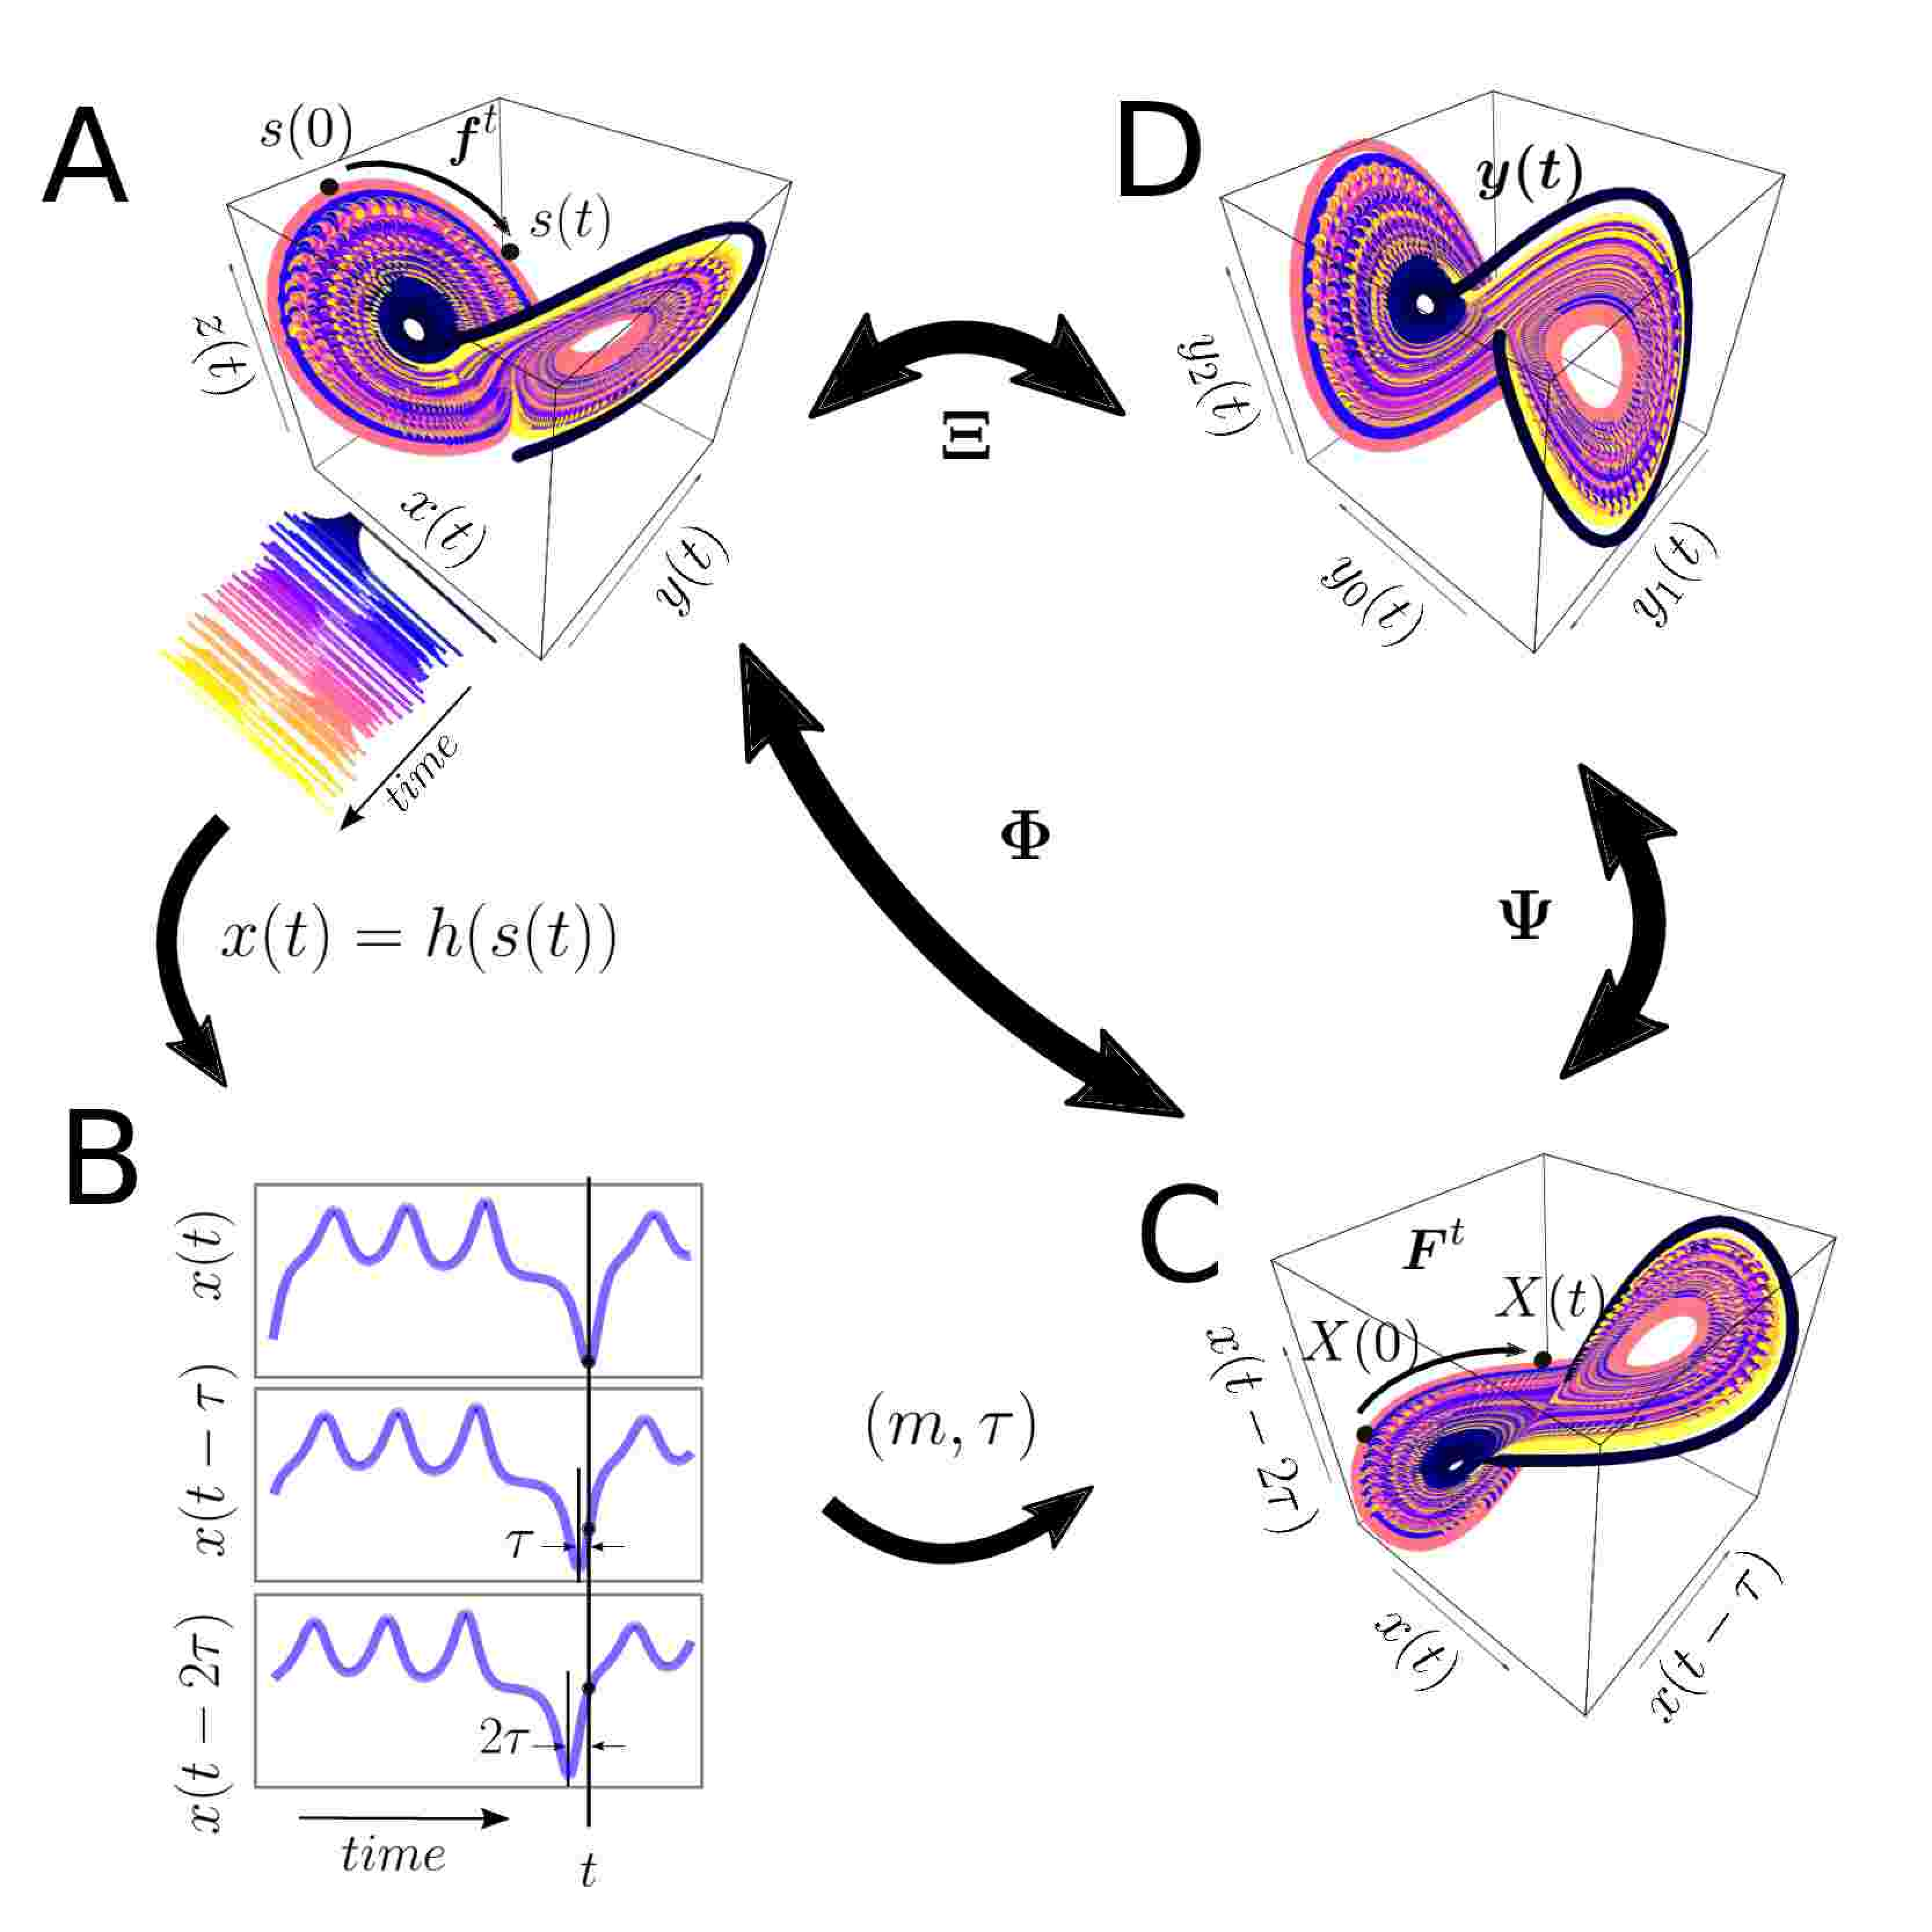
\includegraphics[width=1.0\textwidth]{fig-rss.pdf}
    \caption{
	{\bf State space reconstruction methodology.}
	State space reconstruction is based on $x(t)=h[s(t)]= h[f^t [s(0)]]$
	where $f^t$ is the true dynamical system, $s(t)$ indicates the state,
    	$s$, at time, $t$,  and $h[ ]$ the measurement function. 
    	The time-delay embedding represented as the $\Phi$, maps the original
    	$d-$dimensional state $s(t)$ into the $m-$dimensional uniform 
	time-delay embedding matrix $\boldsymbol{X}(t)$.
    	The transformation map $\Psi$ then maps $\boldsymbol{X}(t)$ into 
	a new state $y(t)$ of dimensions $n < m$.
    	(A) $M-$dimensional manifold representing the state space 
	(e.g. Lorenz system);
    	(B) Delayed copies of $1-$dimensional $x(t)$ from the Lorenz system;
   	(C) $m-$dimensional reconstructed state space with 
    	\texorpdfstring{$m$}{m} and    \texorpdfstring{$\tau$}{T}, and 
    	(D) $y(t)$ is the $n-$dimensional reconstructed state space.
	The total reconstruction map is represented as $\Xi = \Psi \circ \Phi $
	where $\Phi$ is the delay reconstruction map and 
	$\Psi$ is the coordinate transformation map.
	This figure is adapted from 
   	\cite{Quintana-Duque2012, casdagli1991, uzal2011}.
	Code and data to reproduce the figure is available in \cite{srep2020}.
    }
    \label{fig:ssr}
\end{figure}
%%---------------------------------(FIGURE)-------------------------------------



\subsection*{Uniform Time-Delay Embedding (UTDE)}\label{sec:utimedelayembedding}
Frank et al. and Sama et al. refer to the state space reconstruction
as "time-delay embeddings" or "delay coordinates" \cite{frank2010, sama2013}. 
However, we consider the term "uniform time-delay embedding"
as more descriptive and appropriate terminology for our work.
Hence, the uniform time-delay embedding is represented as a matrix of uniform delayed 
copies of the time series $\{ \boldsymbol{x}_n \}_{n=1}^N$ where $N$ is 
the sample length of $\{ \boldsymbol{x}_n \}$ and $n$ is index for the 
samples of $\{ \boldsymbol{x}_n \}$.
$\{ \boldsymbol{x}_n \}_{n=1}^N$ has a sample rate of $T$.
The delayed copies of $\{ \boldsymbol{x}_n \}$ are uniformly separated by $\tau$
and represented as $\{\boldsymbol{ \tilde{x} }_{n- i\tau} \}$
where $i$ goes from $0,1, \dots, (m-1)$.
Generally speaking, $\{\boldsymbol{ \tilde{x} }_{n- i\tau} \}$ contains
information of unobserved state variables and encapsulates the information of
the delayed copies of the available time series in the uniform time-delay 
embedding matrix $\boldsymbol{X}^{m}_{\tau}$, 
$\boldsymbol{X}^{m}_{\tau} \in \mathbb{R}^m$, defined as
%%********************************[EQUATION]************************************
\begin{equation}\label{eq:tde}
\boldsymbol{X}^{m}_{\tau}  =
\begin{pmatrix}
\boldsymbol{ \tilde{x} }_n \\
\boldsymbol{ \tilde{x} }_{n-\tau} \\
\boldsymbol{ \tilde{x} }_{n-2\tau} \\
\vdots \\
\boldsymbol{ \tilde{x} }_{n- (m-1) \tau} \\
\end{pmatrix}^\intercal, 
\end{equation}
%%********************************[EQUATION]************************************
where $m$ is the embedding dimension, $\tau$ is the embedding delay and
$ ^\intercal$ denotes the transpose.
$m$ and $\tau$ are known as embedding parameters.
The matrix dimension of $ \boldsymbol{X}_{\tau}^{m} $ is defined by
$N-(m-1)\tau$ rows and $m$ columns and 
$N-(m-1)\tau$ defines the length of each delayed copy 
of $\{ \boldsymbol{ \tilde{x} }_n \}$ in $\boldsymbol{X}^{m}_{\tau}$.
%For further details and explicit examples of uniform time-delay 
%embedding methodology, we refer the reader to the \nameref{S1_AppendixA}.




\subsection*{Estimation of Embedding Parameters}
The estimation of the embedding parameters ($m$ and $\tau$) 
is a fundamental step for the state space reconstruction with the use
of uniform time-delay embedding method.
With this in mind, we review two of the most common algorithms,
which will be used in our work, to compute the embedding
parameters: the false nearest neighbour (FNN) and the average mutual information (AMI).

%%%%%%%%%%%%%%%%%%%%%%%%%%%%%%%%%%%%%%%%%%%%%%%%%%%%%%%%%%%%%%%%%%%%%%%%%%%%%%%%
%*******************************************************************************
\subsubsection*{False Nearest Neighbours}
To select the minimum embedding dimension $m_0$, Kennel et al. \cite{kennel1992}
used the method of false neighbours which can be understood as follows:
on the one hand, when the embedding dimension is too small to unfold the 
attractor "not all points that lie close each other will be neighbours and 
some points appear as neighbours because of the attractor has been projected 
down into an smaller space", on the other hand, when increasing the embedding 
dimension "points that are near to each other in the sufficient
embedding dimension should remain close as the dimension increase from $m$ 
to $m+1$ \cite{krakovska2015}".
From a mathematical point of view, the state space reconstruction theorem is 
done when the attractor is unfolded with either the minimum embedding 
dimension, $m_0$, or any other embedding dimension value where 
$m \ge m_0$ \cite{kennel1992}. On the contrary, any large value of $m_0$ 
leads to excessive computations \cite{bradley2015}. With this in mind, 
Cao \cite{Cao1997} proposed an algorithm based on the false neighbour method 
where only the time-series and one delay embedding value are necessary 
to select the minimum embedding dimension. Cao's algorithm is based 
on $E(m)$  which is the mean value of all $a(i,m)$, both defined as follows
%%********************************[EQUATION]************************************
\begin{equation}\label{eq:e}
  \begin{aligned}
	E(m) &= \frac{1}{N-m\tau} \sum_{i=1}^{N-m\tau} a(i,m) \\
	 &=
       \frac{1}{N-m\tau} \sum_{i=1}^{N-m\tau}
       \frac{ || \boldsymbol{X}_i(m+1) - \boldsymbol{X}_{n(i,m)}(m+1) || }
            { || \boldsymbol{X}_i(m) - \boldsymbol{X}_{n(i,m)}(m) ||  }
  \end{aligned}
\end{equation}
%%********************************[EQUATION]************************************
where $\boldsymbol{X}_i(m)$ and $\boldsymbol{X}_{n(i,m)}(m)$ are the time-delay
embeddings with $i=1,2,\dots,N-(m-1)\tau$ and $ n(i,m)= 1 \le n(i,m) \le N-m\tau$.
From Eq.~\ref{eq:e}, it can be seen that $E(m)$ is only dependent on $m$ 
and $\tau$ for which $E_1(m)$ is defined as
%%********************************[EQUATION]************************************
\begin{equation}\label{eq:e1}
E_1(m) = \frac{ E(m+1) } { E(m)}.
\end{equation}
%%********************************[EQUATION]************************************
$E_1(m)$ is therefore considered to investigate the variation from $m$ to $m+1$
in order to find the minimum embedding dimension $m_0$ (Eq.~\ref{eq:e1}).
As described in \cite{Cao1997}: "$E_1(m)$ stops changing when $m$ is greater
than some $m_0$, if the time series comes from a multidimensional state space
then $m_0 + 1$ is the minimum dimension".
Additionally, Cao proposed $E_2(m)$ to distinguish deterministic signals from
stochastic signals. $E_2(m)$ is defined as
%%********************************[EQUATION]************************************
\begin{equation}\label{eq:e2}
E_2(m) = \frac{ E^* (m+1) } { E^*(m)},
\end{equation}
%%********************************[EQUATION]************************************
where
%%********************************[EQUATION]************************************
\begin{equation}\label{eq:ee}
E^*(m) = \frac{1}{N-m\tau} \sum_{i=1}^{N-m\tau}
|  \boldsymbol{X}_i(m+1) - \boldsymbol{X}_{n(i,m)}(m+1) |.
\end{equation}
%%********************************[EQUATION]************************************
For instance, when the signal comes from random noise (values that are 
independent from each other), all $E_2(m)$ values are approximately equal 
to 1 (e.g. $E_2(m) \approx 1$). However, for deterministic data $E_2(m)$ is 
not constant for all $m$ (e.g. $E_2(m) \neq 1$).

As an example of the use of $E_1(m)$ and $E_2(m)$ values, we consider two time 
series: the solution for the $x$ variable of the Lorenz system 
(Fig~\ref{fig:caoami}A), and a Gaussian noise time series with zero mean 
and a variance of one (Fig~\ref{fig:caoami}B).
We then compute $E_1(m)$ and $E_2(m)$ values for each time series.
The $E_1(m)$ values for the chaotic time series appear to be constant
after the dimension is equal to six.
The determination of six is given that any value of $m$ can be used as they 
are within the threshold of $1\pm0.05$ (Fig~\ref{fig:caoami}C).
$E_2(m)$ values, for chaotic time series, are different to one 
(Fig~\ref{fig:caoami}E), for which, it can be concluded that for the 
chaotic time series the minimum embedding dimension the time series 
comes from a deterministic signal. With regard to the noise time series,  
$E_1(m)$ values appeared to be constant when $m$ is close to thirteen, 
which is defined by the threshold of $1\pm0.05$ (Fig~\ref{fig:caoami}D).
$E_1(m)$ values then indicate the minimum embedding dimension of the 
noisy time series is thirteen, however all of the $E_2(m)$ values are 
approximately equal to one (Figure~\ref{fig:caoami}F) for which it can be 
concluded that noise time series is a stochastic signal.
It is important to note that for this work not only $E_1(m)$ and $E_2(m)$ are 
computed but also a variation of $\tau$ from 1 to 20 is presented. 
The purpose of such variation for $\tau$ is to show its independence with
regard to $E_1(m)$ and $E_2(m)$ values as $\tau$ is increasing 
(Fig~\ref{fig:caoami}C,D,E and F). 
However, one negative of the Cao's algorithm \cite{Cao1997} is the definition of 
a new threshold where $m$ values appear to be constant in $E_1 (m)$.
In the case of the given examples and reported results, we defined such 
threshold as 0.05. Further investigation is required for the selection of the 
threshold in the $E_1(m)$, as the selection of the threshold in this work is 
base on no particular method but visual inspection.

%%%%%%%%%%%%%%%%%%%%%%%%%%%%%%%%%%%%%%%%%%%%%%%%%%%%%%%%%%%%%%%%%%%%%%%%%%%%%%%%
%*******************************************************************************
\subsubsection*{Average Mutual Information}
When selecting the delay dimension parameter, $\tau$, one can consider the 
following two cases:
(i) when $\tau$ is too small, the elements of time-delay embedding will be along
the bisectrix of the phase space and the reconstruction is generally not 
satisfactory, 
(ii) on the contraty, when $\tau$ is too large the elements of the uniform 
time-delay embedding will become spread and uncorrelated which makes 
recovering the underlying attractor more difficult if not 
impossible \cite{casdagli1991, emrani2014a, garcia2005e71}.
With regard to the algorithms to compute $\tau$, 
Emrani et al. \cite{emrani2014a}, for instance, used the autocorrelation 
function in which the first zero crossing is considered as the minimum delay 
embedding parameter. However, the autocorrelation function is a linear 
statistic over which the Average Mutual Information (AMI) algorithm is 
preferred because the AMI takes into account the nonlinear dynamical 
correlations \cite{afraser1986,krakovska2015}. With this in mind, the AMI 
algorithm is described below to estimate the minimum delay embedding 
parameter, \texorpdfstring{$\tau_0$}{T}.

To compute the AMI, an histogram of $x(n)$ using $n$ bins is calculated
and then a probability distribution of data is computed \cite{kantz2003}.
AMI is therefore denoted by $I(\tau)$ which is the average mutual 
information between the original time series, $x(n)$, and the delayed 
time series, $x(n-\tau)$, delayed by $\tau$ \cite{kabiraj2012}. 
AMI is defined by
%%********************************[EQUATION]************************************
\begin{equation}\label{eq:ami}
I(\tau) = \sum_{i,j}^N p_{ij} log_2 \frac{ p_{ij} }{ p_i p_j }.
\end{equation}
%%********************************[EQUATION]************************************
Probabilities are defined as follows:
$p_i$ is the probability that $x(n)$ has a value inside the $i$-th bin of 
the histogram, $p_j$ is the probability that $x(n+\tau)$ has a value inside 
the $j$-th bin of the histogram and $p_{ij}(\tau)$ the probability 
that $x(n)$ is in bin $i$ and $x(n+\tau)$ is in bin $j$. The AMI is measured 
in bits (base 2, also called shannons) \cite{kantz2003, nonlinearTseries2016}.
For small $\tau$, AMI will be large and it will then decrease more or 
less rapidly. As $\tau$ increase and goes to a large limit, 
$x(n)$ and $x(n+\tau)$ have nothing to do with each other and $p_(ij)$ is 
factorised as $p_ip_j$ for which AMI is close to zero. Then, in order 
to obtain $\tau_0$, "it has to be found the first minimum of $I(\tau)$ 
where $x(n+\tau)$ adds maximal information to the knowledge from $x(n)$, or,
where the redundancy is the least" \cite{kantz2003}.

For example, we compute the AMI for two time series:
A) the $x$ solution of the Lorenz system, and
B) a noise time series using a normal distribution with mean zero and 
standard deviation equal to one. From Fig~\ref{fig:caoami}(G, H), it can then be 
concluded that the amount of knowledge for any noise time series is zero 
for which the first minimum embedding parameter is $\tau_0=1$. 
On the contrary, the first minimum of the AMI for the chaotic time series 
is $\tau_0=17$ which is the value that maximize the independence 
between $x(n)$ and $x(n+\tau)$ in the reconstructed state space 
\cite{bradley2015}.
%%---------------------------------(FIGURE)-------------------------------------
Similarly as Cao's algorithm negatives, AMI's algorithm is not an
exception for negatives, which are worthwhile to mention for further 
investigations.
For instance, (i) is not clear why the choose of the first minimum of the AMI 
is the minimum delay embedding parameter \cite{kantz2003} and 
(ii) the probability distribution of the AMI function is computed
with the use of histograms which depends on a heuristic choice of number of bins
for which AMI depends on partitioning \cite{garcia2005e71}.

%%---------------------------------(FIGURE)-------------------------------------
\begin{figure}[ht]
\centering
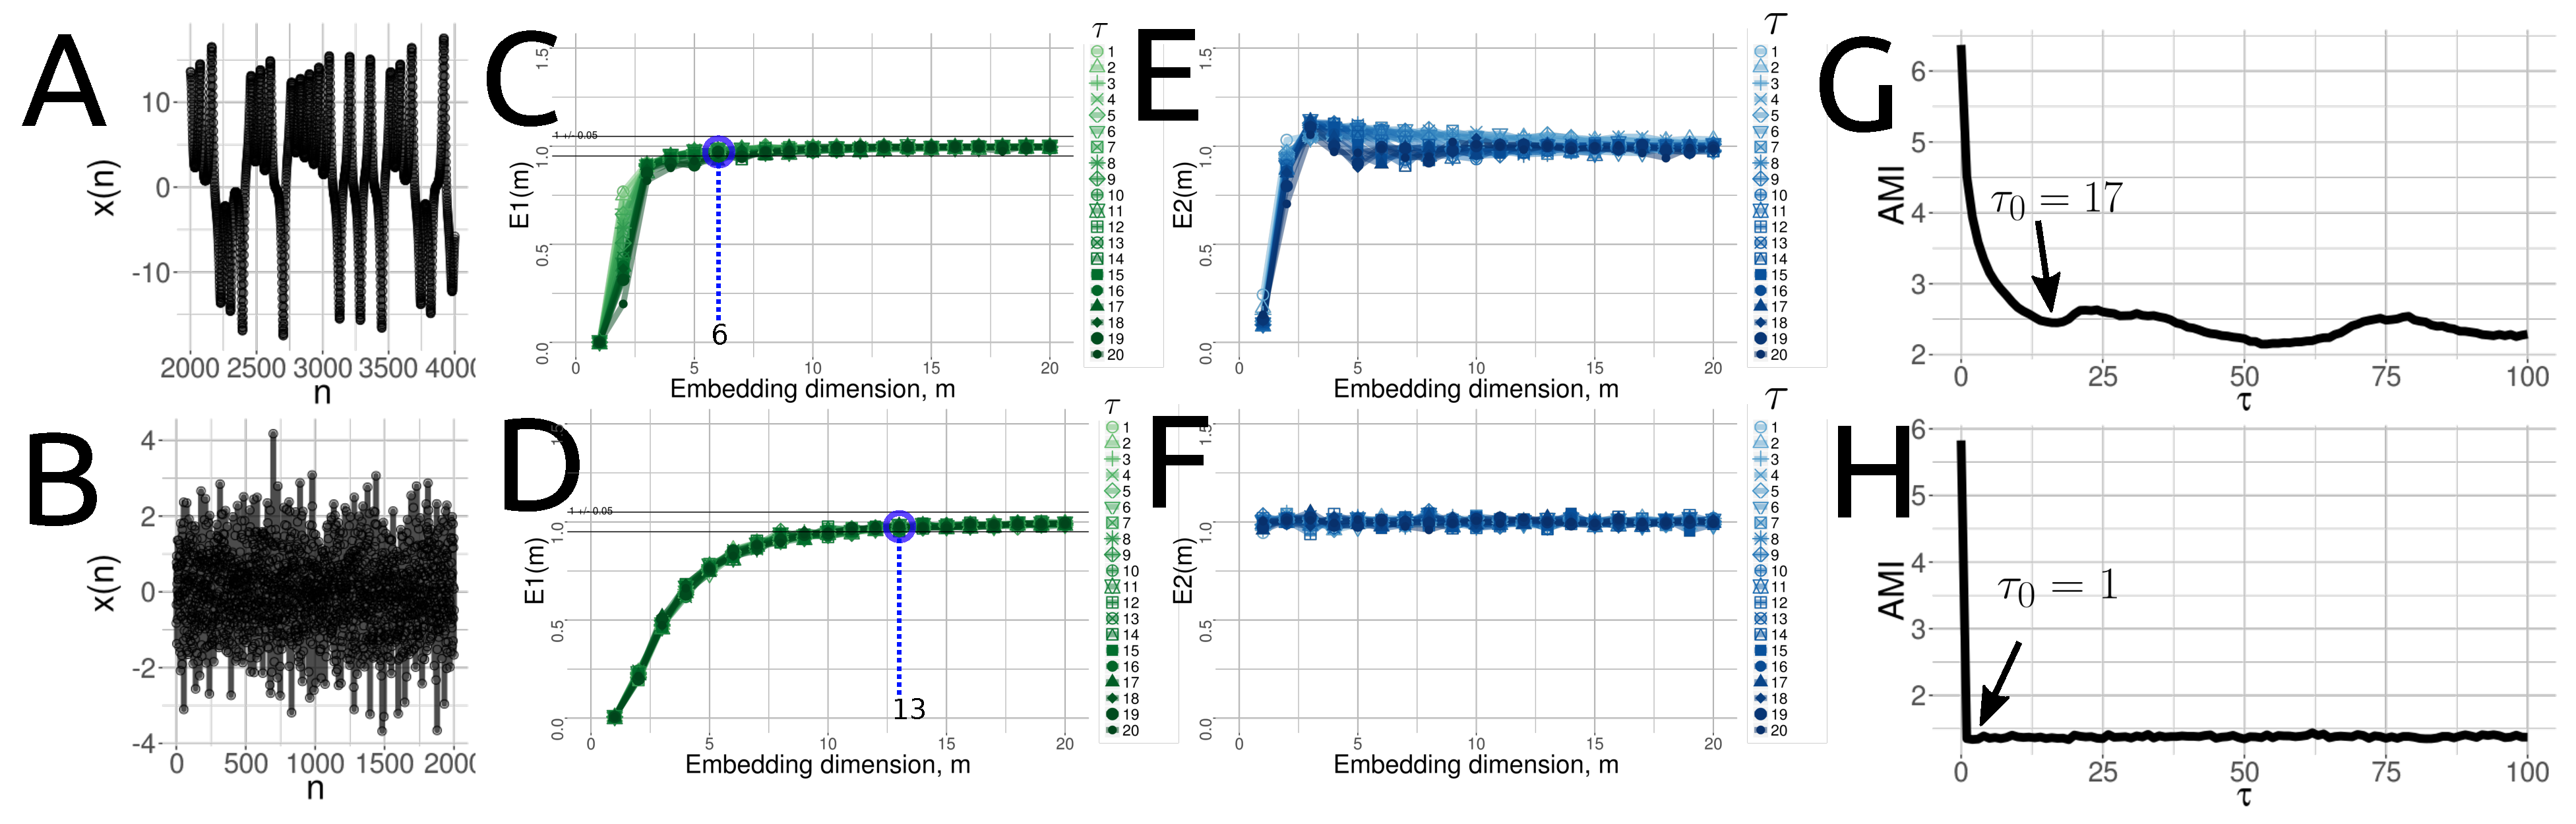
\includegraphics[width=1.0\textwidth]{fig-caoami.pdf}
    \caption{
	{\bf Minimum delay embedding values with AMI's method and minimum dimension embedding values with Cao's method.} 
	(A) chaotic and (B) random time series.
	(C, D) $E_1 (m)$ values and (E, F) $E_2(m)$ values 
	with variations of $\tau$ values from one to twenty
	for chaotic and random time series.
	(G, H) AMI values where its first minimum value in the curve
	is the minimum time delay embedding ($\tau_0$).
	Code and data to reproduce the figure is available in \cite{srep2020}.
        }
    \label{fig:caoami}
\end{figure}
%%---------------------------------(FIGURE)-------------------------------------


%*******************************************************************************
\section*{Recurrence Quantification}\label{sec:recurrence-quantification}
\subsection*{Recurrence Plots}
Originally, Henri Poincar\'e in 1890 introduced the concept of recurrences 
in conservative systems, however such discovery was not put into practice 
until the development of faster computers \cite{marwan2007},
for which Eckmann et al. \cite{eckmann1987} in 1987 introduced a method
where recurrences in the dynamics of a system can be visualised using 
Recurrence Plots. The intention of Eckmann et al. \cite{eckmann1987} was to 
propose a tool, called Recurrence Plot (RP), that provides insights into 
high-dimensional dynamical systems where trajectories are very difficult to 
visualise. Therefore, "RP helps us to investigate the 
$m-$dimensional phase space trajectories through a two-dimensional 
representation of its recurrences" \cite{marwan2015}.
Similarly, Marwan et al. \cite{marwan2015} pointed out that additionally 
to the methodologies of the state space reconstruction and other dynamic 
invariants such as Lyapunov exponent, Kolmogorov-Sinai entropy, 
the recurrences of the trajectories in the phase space can provide 
important clues to characterise natural process that present, for
instance, periodicities (as Milankovitch cycles) or irregular cycles 
(as El Ni\~no Southern Oscillation). 
Such recurrences can not only be presented visually using Recurrence Plots (RP) 
but also be quantified with Recurrence Quantification metrics, which leads 
to applications of these in various areas such as economy, physiology, 
neuroscience, earth science, astrophysics and engineering \cite{marwan2007}.

For the creation of a recurrence plot based on time series 
$\{ \boldsymbol{x}_n \}$, it is first computed the state space 
reconstruction with uniform time-delay embedding 
$X(i)=\{ \boldsymbol{ \tilde{x} }_n, \dots,  
\boldsymbol{ \tilde{x} }_{n -(m-1)\tau} \}$
where $i=1,\dots,N$, $N$ is the number of considered states of $X(i)$ 
and $X(i) \in \mathbb{R}^m$ \cite{eckmann1987}.
The recurrence plot is therefore a two-dimensional $N \times N$ square 
matrix, $\mathbf{R}$, where a black dot is placed at $(i,j)$ 
whenever $X(i)$ is sufficiently close to $X(j)$: 
%%********************************[EQUATION]************************************
\begin{equation}
\mathbf{R}^{m}_{i,j} (\epsilon) = \Theta ( \epsilon_i - || X(i) - X(j) ||
\end{equation}
%%********************************[EQUATION]************************************
where $\quad i,j=1,\dots,N$, $\epsilon$ is a threshold distance, 
$|| \cdotp ||$ a norm, and $\Theta(\cdotp)$ is the Heaviside 
function (i.e. $\Theta(x)=0$, if $x<0$, and $\Theta(x)=1$ otherwise) 
(Fig~\ref{fig:rps}(A,B)) \cite{eckmann1987, marwan2007,marwan2015}.
RP is also characterised with a line of identity (LOI) which is a  
diagonal line due to $ R_{i,j}=1 (i,j=1,\dots,N)$. 


%*******************************************************************************
%*******************************************************************************
%*******************************************************************************
\subsection*{Structures of Recurrence Plots}
Pattern formations in the RPs can be designated either 
as topology for large-scale patterns or texture for small-scale patterns.
In the case of topology, the following pattern formations are commonly presented:
(i) homogeneous where uniform recurrence points are spread in the RP e.g., 
uniformly distributed noise (Fig~\ref{fig:rps}C), 
(ii) periodic and quasi-periodic systems where diagonal lines and 
checkerboard structures represent oscillating systems, e.g., sinusoidal 
signals (Fig~\ref{fig:rps}D), 
(iii) drift where paling or darkening recurrence points away from 
the LOI is caused by drifting systems, 
e.g., logistic map (Fig~\ref{fig:rps}E), and
(iv) disrupted where recurrence points are presented white areas or 
bands that indicate abrupt changes in the dynamics, e.g. Brownian motion 
(Fig~\ref{fig:rps}F) \cite{eckmann1987, marwan2015}.
Texture patterns in RPs can be categorised as:
(i) single or isolated recurrence points that represent rare occurring states, 
and do not persist for any time or fluctuate heavily,
(ii) dots forming diagonal lines where the length of the small-scale parallel 
lines in the diagonal are related to the ratio of determinism or predictability 
in the dynamics of the system, and
(iii) dots forming vertical and horizontal lines where the length of the 
lines represent a time length where a state does not change or change very 
slowly and these patterns formation represent discontinuities in the signal, 
and (iv) dots clustering to inscribe rectangular regions which are related 
to laminar states or singularities \cite{marwan2015}.

Although, each of the previous pattern descriptions of the structures in the 
RP offer an idea of the characteristics of dynamical systems, 
these might be misinterpreted and conclusions might tend to be subjective 
as these require the interpretation of a particular researcher(s).
Because of that, recurrence quantification analyis (RQA) offer objective 
methodologies to quantify such visual characteristics of previous 
recurrent pattern structures in the RP \cite{zbilut1992}.

%---------------------------------(FIGURE)-------------------------------------
\begin{figure}[ht]
\centering
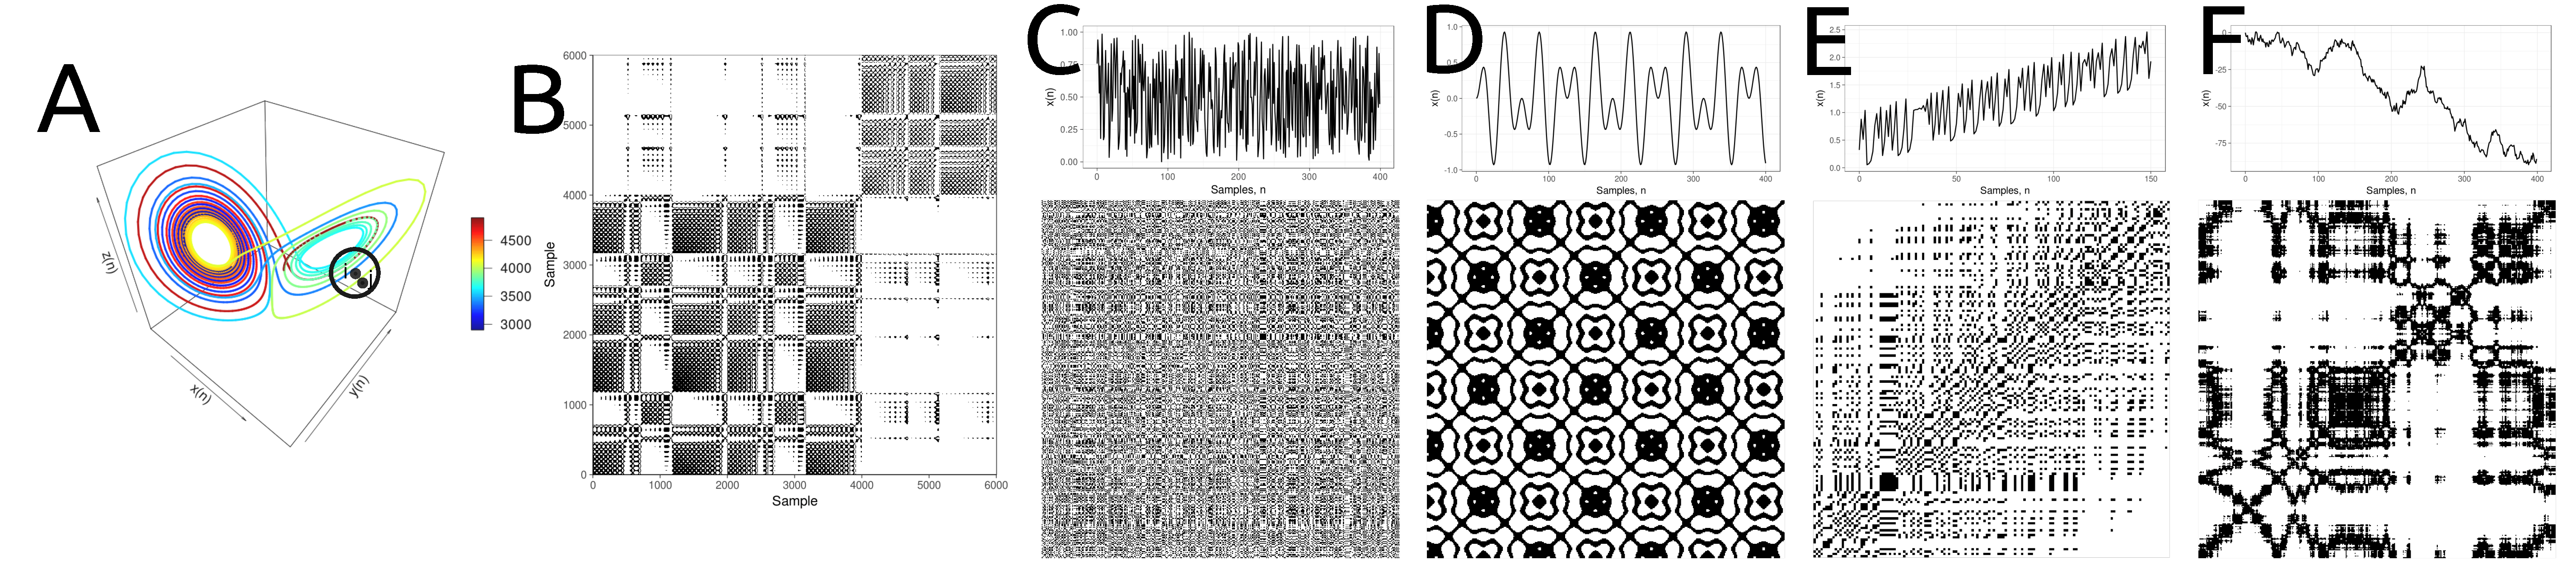
\includegraphics[width=1.0\textwidth]{fig-rps.pdf}
    \caption{
	{\bf Recurrence Plots and its patterns.} 
	(A) State space of the Lorenz system with controlling parameters 
	($\rho=28, \sigma=10, \beta=8/3$) where the point, $j$, in trajectory $X()$ which falls into the neighborhood 
	(black circle) of a given point at $i$ is a recurrent point and is 
	represented as a black dot in the recurrence plot at location 
	$(i, j)$ or white otherwise.
	(B) Recurrence plot using the 
	three components of the Lorenz system and the RP with no embeddings 
	and threshold $\epsilon=5$.
	Time-series with its respective recurrence plot for:
	(C) uniformly distributed noise,
	(D) super-positionet harmonic oscillation 
	($sin( \frac{1}{5}*t) * sin( \frac{5}{100}*t) $),
	(E) drift logistic map ($x_{i+1} = 4 x_i (1- x_i) $) corrupted 
	with a linearly increase term ($0.01*i$), and
	(F) disrupted brownian motion  ($x_{i+1} = x_i + 2*rnorm(1) $).
	This figure is adapted from \cite{marwan2015}.
	Code and data to reproduce the figure is available in \cite{srep2020}.
	}
    \label{fig:rps}
\end{figure}
%%---------------------------------(FIGURE)-------------------------------------



%*******************************************************************************
\subsection*{Recurrence Quantifications Analysis (RQA)}
Originally, Zbilut et al. \cite{zbilut1992} proposed metrics to investigate 
the density of recurrence points in RPs, then histograms of lengths for 
diagonal lines in RPs were studied by \cite{trulla1996} which were the 
introduction to the term recurrence quantification analysis (RQA) 
\cite{marwan2008}. RQA has been applied in many fields such as life science, 
engineering, physics, and others \cite{marwan2008}. Particularly in human 
movement to investigate noise and complexity of postural control 
\cite{rhea2011}, postural control \cite{apthorp2014} or interpersonal 
coordination \cite{duran2017}. The success of RQA is not only due to its 
simple algorithmic implementation but also to its capacity to detect tiny 
modulations in frequency or phase which are not detectable using standard 
methods e.g. spectral or wavelet analysis \cite{marwan2011}, and that 
RQA's metrics are quantitatively and qualitatively independe]nt of embedding 
dimension which is verified experimentally by \cite{iwanski1998}.
RQA metrics comprehend percentage of recurrence, percentage of determinism, 
ratio, Shannon entropy of the frequency distributions of the line lengths,
maximal line length and divergence, trend and laminariy 
\cite{marwan2007, marwan2015}. For this work, we considered only four 
RQA metrics, due to its consistency with our preliminary experiments, 
which are described below. Such metrics are computed the nonlinearTseries 
R package \cite{nonlinearTseries2016}.

\subsubsection*{REC values}
The percentage of recurrence (REC) is defined as
%%********************************[EQUATION]************************************
\begin{equation}
REC(\epsilon,N) = 
		\frac{1}{N^2 - N} \sum^{N}_{i \neq j = 1} 
		\mathbf{R}^{m}_{i,j}(\epsilon),
\end{equation}
%%********************************[EQUATION]************************************
which enumerates the black dots in the RP excluding the line of identity.
REC is a measure of the relative density of recurrence points in the sparse 
matrix \cite{marwan2015}.
%REC is computed as follow with the nonlinearTseries package 
% \cite{nonlinearTseries} 
%  hist = getHistograms(neighs, ntakens, lmin, vmin)
%  # calculate the number of recurrence points from the recurrence rate. The
%  # recurrence rate counts the number of points at every distance in a concrete
%  # side of the main diagonal.
%  # Thus, sum all points for all distances, multiply by 2 (count both sides) and
%  # add the maindiagonal
%  numberRecurrencePoints = sum(hist$recurrenceHist) + ntakens
%  # calculate the recurrence rate dividing the number of recurrent points at a
%  # given distance by all points that could be at that distance
%  recurrence_rate_vector = 
%  hist$recurrenceHist[1:(ntakens - 1)] / ((ntakens - 1):1)
%  # percentage of recurrent points
%  REC = (numberRecurrencePoints) / ntakens ^ 2

\subsubsection*{DET values} 
The percent determinism (DET) is defined as the fraction of recurrence points
that form diagonal lines and it is determined by
%%********************************[EQUATION]************************************
\begin{equation}
DET=
	\frac{\sum^{N}_{l=d_{min}} l H_D{l} }
	     {\sum^{N}_{i,j=1} \mathbf{R}_{i,j}(\epsilon) },
\end{equation}
%%********************************[EQUATION]************************************
where 
%%********************************[EQUATION]************************************
\begin{equation}
H_D(l) = 
	\sum^{N}_{i,j=1} 
	(1- \mathbf{R}_{i-1,j-1}(\epsilon) ) 
	(1- \mathbf{R}_{i+l,j+l}(\epsilon) ) 
	\prod^{l-1}_{k=0}  \mathbf{R}_{i+k,j+k}(\epsilon)
\end{equation}
%%********************************[EQUATION]************************************
is the histogram of the lengths of the diagonal structures in the RP.
DET can be interpreted as the predictability of the system for periodic signals 
which, in essence, have longer diagonal lines than the short diagonals lines
for chaotic signals or absent diagonal lines for stochastic signals 
\cite{marwan2007, marwan2015}. Similarly, DET is considered as a measurement for 
the organisation of points in RPs  \cite{iwanski1998}. 
%percent determinism (DET) is computed as follow with the nonlinearTseries 
%package \cite{nonlinearTseries}  
% calculateDiagonalParameters = function(ntakens, numberRecurrencePoints,
%                                       lmin = 2, lDiagonalHistogram,
%                                       recurrence_rate_vector, maxDistanceMD) {
%  #begin parameter computations
%  num = sum((lmin:ntakens) * lDiagonalHistogram[lmin:ntakens])
%  DET = num / numberRecurrencePoints


\subsubsection*{RATIO values}
RATIO is defined as the ratio between DET and REC and it is calculated from 
the frequency distributions of the lengths of the diagonal lines.
RATIO is useful to discover dynamic transitions \cite{marwan2015}.
%  diagP = calculateDiagonalParameters(
%    ntakens, numberRecurrencePoints, lmin, hist$diagonalHist,
%    recurrence_rate_vector, maxDistanceMD
%  )
% calculateDiagonalParameters = function(ntakens, numberRecurrencePoints,
%                                       lmin = 2, lDiagonalHistogram,
%                                       recurrence_rate_vector, maxDistanceMD) {
%  #begin parameter computations
%  num = sum((lmin:ntakens) * lDiagonalHistogram[lmin:ntakens])
%  DET = num / numberRecurrencePoints
% 
%
%    RATIO = diagP$DET / REC
%

\subsubsection*{ENT values}
ENT is the Shannon entropy of the frequency distribution of the diagonal 
line lengths and it is defined as
%%********************************[EQUATION]************************************
\begin{equation}
ENT= - \sum^{N}_{l=d_{min}} p(l) ln p(l) \quad with 
	\quad p(l)=\frac{ H_D(l) }{ \sum^{N}_{ l=d_{min} } H_D(l) }.
\end{equation}
%%********************************[EQUATION]************************************
ENT reflects the complexity of the deterministic structure in the system.
For instance, for uncorrelated noise or oscillations, 
the value of ENT is rather small and indicates low complexity of the system,
therefore "the higher the ENT is the more complex the dynamics are" 
\cite{marwan2007, marwan2015}.
%#'  \item \emph{ENTR}: Shannon entropy of the diagonal line lengths distribution
%
%calculateDiagonalParameters = function(ntakens, numberRecurrencePoints,
%                                       lmin = 2, lDiagonalHistogram,
%                                       recurrence_rate_vector, maxDistanceMD) {
%
%  pl = lDiagonalHistogram / sum(lDiagonalHistogram)
%  diff_0 = which(pl > 0)
%  ENTR = -sum(pl[diff_0] * log(pl[diff_0]))

 
\subsection*{Sensitivity and robustness of RPs and RQA.}
RP and RQA are a very young field in nonlinear dynamics and many questions 
are still open, for instance, different parameters for window length size 
of the time series, embedding parameters or recurrence threshold can 
generate different results in RQA's metrics \cite{marwan2011, eckmann1987}.

The selection of recurrence threshold, $\epsilon$, can depend on the system 
that is analysed. For instance, when studying dynamical invariants $\epsilon$ 
require to be very small, for trajectory reconstruction $\epsilon$ requires 
to have a large thresholds or when studying dynamical transition 
there is little importance about the selection of the threshold 
\cite{marwan2011}. Other criteria for the selection of $\epsilon$ is that 
the recurrence threshold  should be five times larger 
than the standard deviation of the observational noise
or the use of diagonal structures within the RP is suggested in order
to find the optimal recurrence threshold for (quasi-)periodic process 
\cite{marwan2011}.
Similarly, Iwanski et al. \cite{iwanski1998} highlighted the importance 
of choosing the right embedding parameters to perform RQA for which 
many experiments have to be performed using different parameters in order 
to have a better intuition of the nature of the time series and how 
this is represented by using RQA.

With that in mind, this work explores the sensitivity and robustness 
of the window size of time series, embedding parameters for RSS with UTDE 
and recurrence threshold for RP and RQA in order to gain a better insight 
into the underlying time series collected from inertial sensors in the 
context of human-humanoid imitation activities.
%Such changes of recurrence threshold values 
%can modify the patterns in RPs and therefore the values of RQA metrics.
%We therefore computed 3D surfaces to explore the sensibility and robustness of 
%embedding parameters and recurrence threshold in RQA  metrics. Following the 
%same methodology of computing 3D surfaces, we also considered variation of 
%window length size to present RQA metrics dependencies with embedding 
%parameters, recurrence thresholds and window length size.


%Choosing an appropriate recurrence threshold is crucial so as to get 
%meaningful representations in RP and RQA, however, 

%Iwansky et al. \cite{iwanski1998} stated that patterns in Recurrence Plots and 
%metrics for RQA are independent of embedding dimension parameters, 
%however, that is not the case when using 
%different recurrence thresholds. 


%Zbilut et al. \cite{zbilut1992} established RQA metrics with the aim of 
%determining embedding parameters, their method consisted on creating 3D 
%surfaces with RQA metrics with an increase of embedding parameters 
%($m$ and $\tau$), then Zbilut et al. \cite{zbilut1992} explored 
%fluctuations and gradual changes in the 3D surfaces that provide information 
%about the embeddings. Much recently, Marwan et al. \cite{marwan2015} 
%created 3D surfaces for visual selection of not only embedding parameters 
%but also recurrence thresholds. Following same methodologies, we explored 
%the stability and robustness of RQA metrics (REC, DET, RATIO and ENTR)
%using 3D surfaces by an unitary increase of the pair embedding 
%parameters ($0 \ge m \le 10$, $0 \ge \tau \le 10$) and a decimal increase 
%of 0.1 for recurrence thresholds ($ 0.2 \ge \epsilon \le 3 $) 
%(Fig.~\ref{fig:topo_rqas}).



%*******************************************************************************
%*******************************************************************************
%*******************************************************************************
\section*{Experiment} \label{sec:experiment}
We conducted an experiment in the context of human-humanoid imitation (HHI) 
activities where participants were asked to imitate simple horizontal and 
vertical arm movements performed by NAO, a humanoid robot \cite{gouaillier2009}.
Such simple movements were repeated ten times for the participant 
who copied NAO's arm movements in a face-to-face imitation activity.
Also, wearable inertial measurement unit (IMU) sensors were attached 
to the right hand of the participant and to the left hand of the robot 
(Figure~\ref{fig:hri} A,C). Data were then collected with four NeMEMSi 
IMU sensors with sampling rate of 50Hz provinding tri-axial data of the 
accelerometer, gyroscope and magnetometer sensors and quaternions 
\cite{Comotti2014}.
%%---------------------------------(FIGURE)-------------------------------------
\begin{figure}[ht]
  \centering
\includegraphics[width=1.0\textwidth]{fig-hri}
    \caption{
	{\bf Human-humanoid imitation activities.} 
    		Face-to-face human-humanoid imitation (HHI) activities for 
		(A) HHI of horizontal arm movement, 
		(B) Humanoid horizontal arm movement,
		(C) HHI of vertical arm movement, and 
		(D) Humanoid vertical arm movement.
        }
    \label{fig:hri}
\end{figure}
%%---------------------------------(FIGURE)------------------------------------

\subsection*{Participants}
Twenty-three participants,
from now on defined as $pN$ where $N$ is the number of participant, were 
invited to do the experiment. However, data for three participants were 
not used because the instructions for $p01$, who was the only left-handed,
were mistakenly given in a way that movements were performed different
from what had been planned, and for participants $p13$ and $p16$ 
data were corrupted because of problems with Bluetooth communications with sensors. 
With that in mind, data for twenty participants were analysed in this work.
Of the twenty participants, all of them are right-handed healthy participants 
of whom four are females and sixteen are males with a mean and standard 
deviation (SD) age of mean=19.8 (SD=1.39). 

\subsection*{Ethics}
All participants provided informed consent forms prior to participation 
in the experiment. Hence, the experiments were conducted in November 2016 and 
participants confirmed reading and understanding the participant information sheet of the 
experiments and were able to withdraw from the experiment at any time without giving
any reason. The design of the experiments adhered to the University of Birmingham
regulations, data were anonymised and videos were stored only on a 
personal computer in accordance with the Data Protection Act 1998. 
%Refer to Appendix D for further information about the ethics, 
%online participation information sheets and experiment check list.


\subsection*{Human-humanoid imitation activities}
For human-humanoid imitation (HHI) activities four neMEMSi sensors were used,
two of which were attached to the right hand of the participant and the 
other two to the left hand of the humanoid robot.
Then, each participant was asked to imitate repetitions of simple horizontal
and vertical arm movements performed by the humanoid robot in the following 
conditions:
(i) ten repetitions of horizontal arm movement at normal (HN) 
	and faster (HF) speed (Figure~\ref{fig:hri} A), and
(ii) ten repetitions of vertical arm movement at normal (VN) 
	and faster (VF) speed (Figure~\ref{fig:hri} C).
The normal and faster speed of arm movements is defined by the duration 
in number of samples of one repetition of NAO's arm movements. 
We select NAO's arm movements duration to distinguish between normal and 
faster arm movements as NAO's movements have less variation 
for such repetitive movements. 
The duration for one repetition of the horizontal 
arm movement at normal speed, HN, is 5 seconds considering 
that each repetition last around 250 samples.
For horizontal arm movement at faster speed, HF, each repetition were performed 
in 2 seconds which correspond to 90 samples of data.
The vertical arm movement at normal speed, VN, were performed  in 6 seconds 
which is around 300 samples of data. For vertical arm movement at 
faster speed, VF, each repetition lasts about 2.4 seconds which correspond 
to 120 samples of data.
To visualise the distinction between normal and faster speed for horizontal 
and vertical arm movements, Fig~\ref{fig:sts} shows smoothed time series 
for axes Z and Y of the gyroscope sensors with four window lengths: 
2-sec (100-samples), 5-sec (250-samples), 10-sec (500-samples) 
and 15-sec (750-samples).
%%---------------------------------(FIGURE)-------------------------------------
\begin{figure}[ht] 
\centering
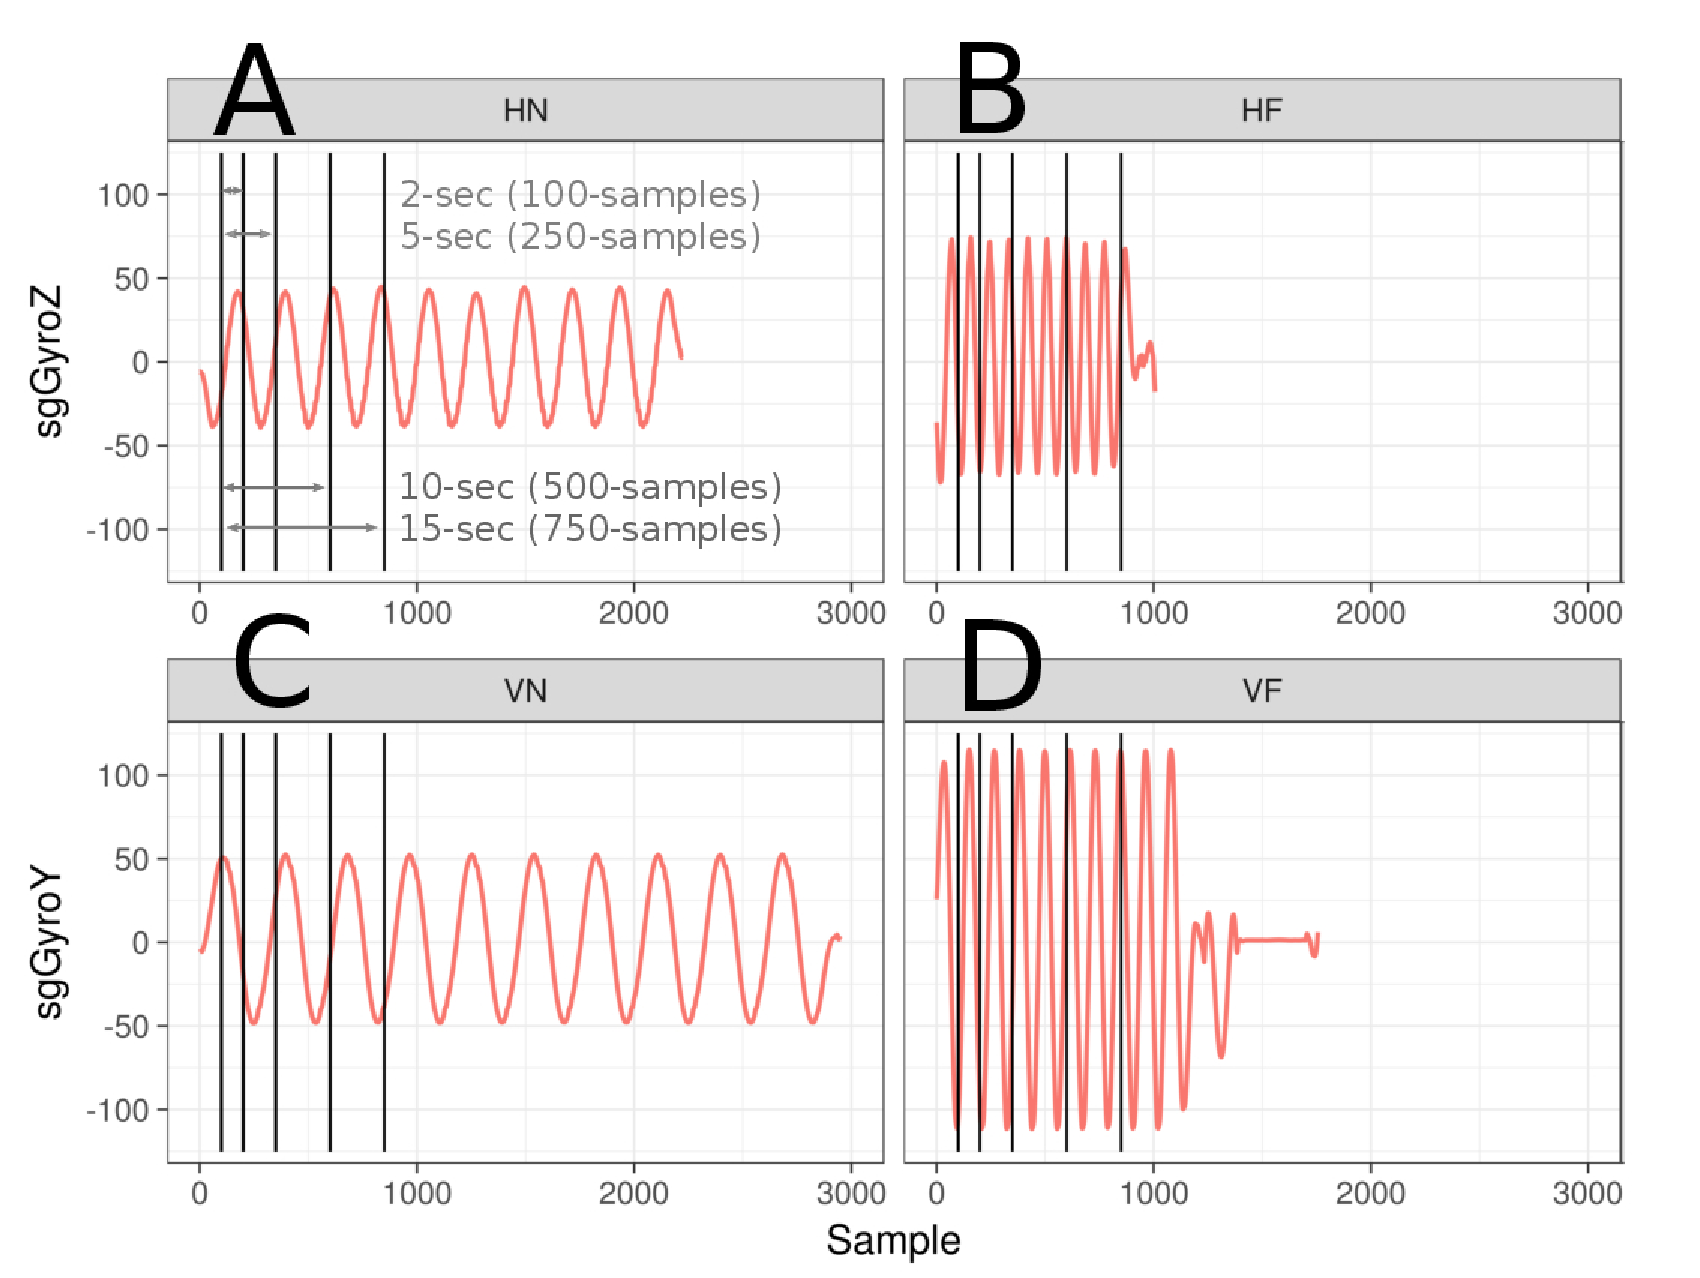
\includegraphics[width=1.0\textwidth]{fig-sts.pdf}
    \caption{
	{\bf Time series duration of horizontal and vertical arm movements.} 
    		Time series of smoothed data from gyroscope sensor 
		for different speed arm movements performed by NAO: 
		(A) Horizontal Normal arm movement (HN), 
		(B) Horizontal Faster arm movement (HF),
		(C) Vertical Normal arm movement (VN) and 
		(D) Vertical Faster arm movement (VF).
		Additionally, 
		(A) shows window sizes for 2-seconds (100 samples), 
		5-seconds (250 samples), 10-seconds (500 samples) 
		and 15-seconds (750 samples)
		which are also presented in (B), (C) and (D).
		Code and data to reproduce the figure is available in \cite{srep2020}.
        }
	\label{fig:sts}
\end{figure}
%%---------------------------------(FIGURE)------------------------------------

\subsection*{Data collection from inertial measurement units} 
\label{sec:experiment:subsec:imu}
To give insight to the research questions, 
we considered various conditions of time series collected for this work: 
\begin{itemize}
\item Three levels of smoothness for normalised data 
	(e.g., sg0zmuv, sg1zmuv and sg2zmuv) where sg 
	stands for Savitzky-Golay filter with two different filter lengths (29 and 159) 
	and the same polynomial degree of 5 using the function \texttt{sgolay(p,n,m)} \cite{Rsignal}
	and zmuv is zero mean unit variance.
\item four arm movement activities with two velocities: 
	horizontal normal (HN), horizontal faster (HF), 
	vertical normal (VN), and vertical faster (VF), and
\item four window lengths: 2-sec (100 samples), 5-sec (250 samples), 
	10-sec (500 samples) and 15-sec (750 samples).
\end{itemize}
%After the data collection, raw time series were windowed, normalised and smoothed. 
Due to space limitations and to have simple visualisation, 
we only present 10-sec (500 samples) window length time series for 
three participants (p01, p01 and p03) performing horizontal 
arm movements (axis GyroZ) and vertical arm movements (axis GyroY) (Figs \ref{fig:ts}).
%%---------------------------------(FIGURE)-------------------------------------
\begin{figure}[ht]
\centering
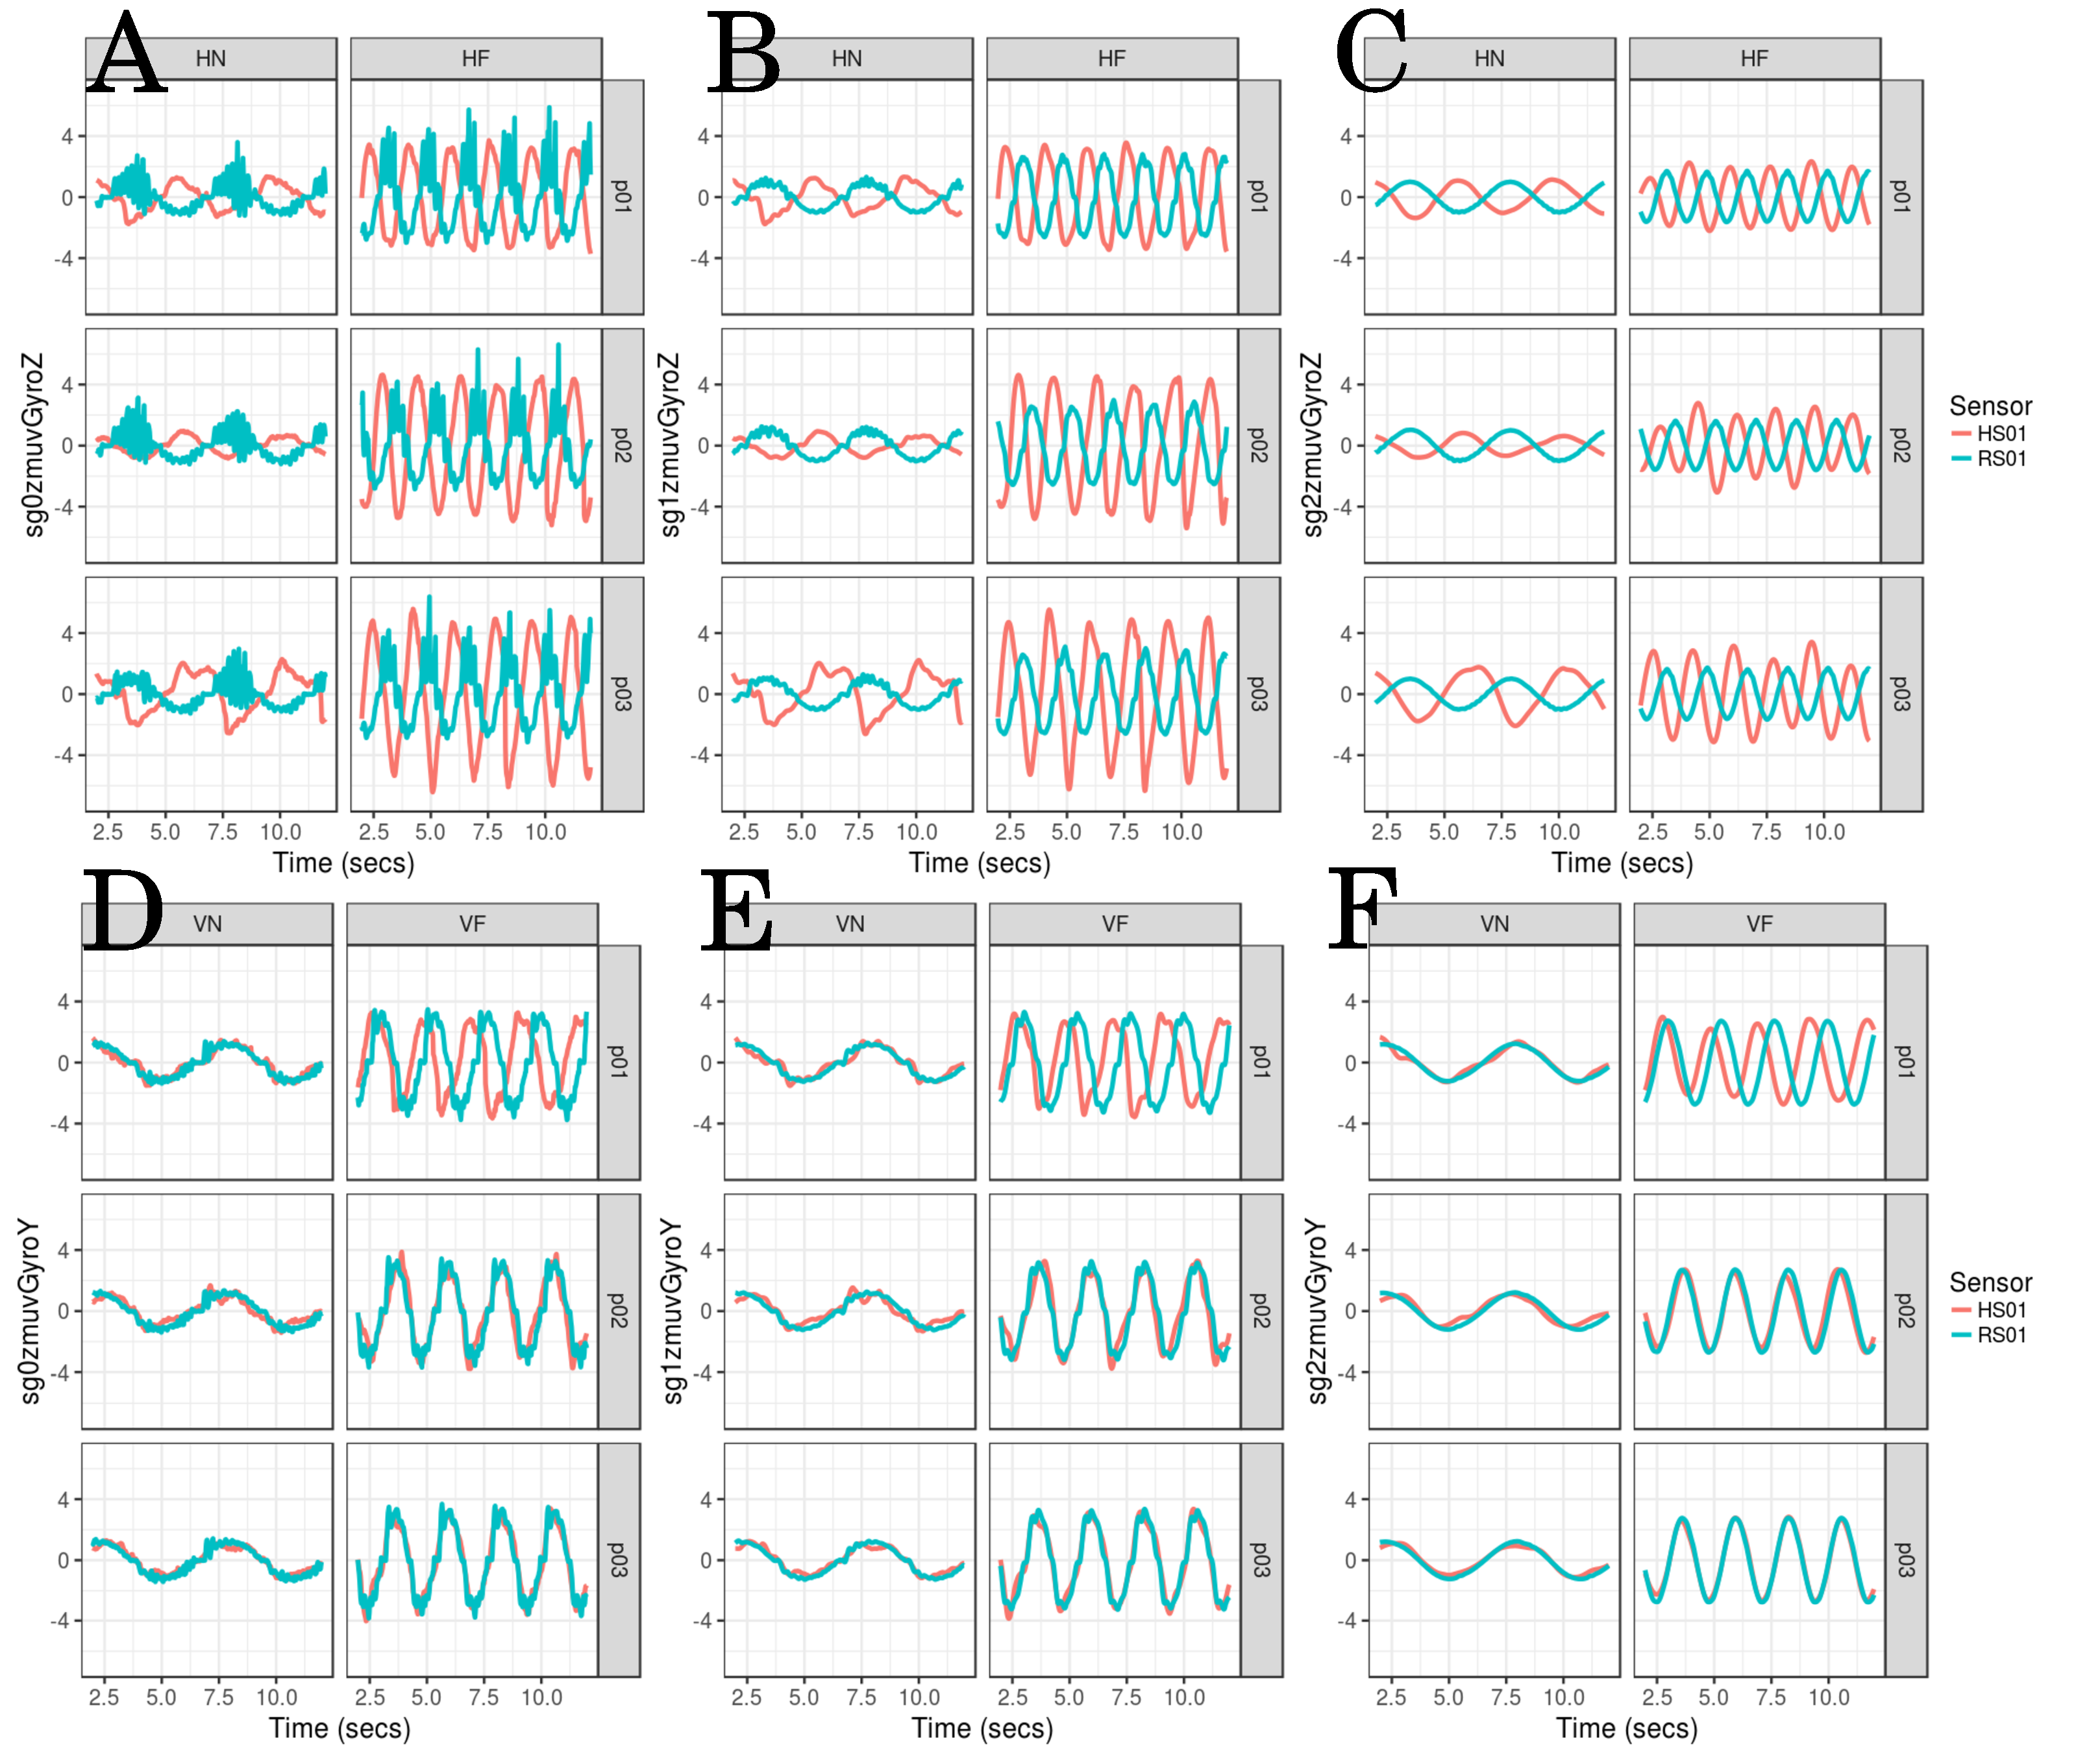
\includegraphics[width=1.0\textwidth]{fig-fig1.pdf}
    	\caption{ 
	{\bf Time series for horizontal and vertical arm movements.}
		(A/D) raw-normalised (sg0zmuv), 
		(B/E) normalised-smoothed 1 (sg1zmuv) and
		(C/F) normalised-smoothed 2 (sg2zmuv).
		Time series are only for three participants 
		($p01$, $p02$, and $p03$) 
		for horizontal and vertical arm movements in normal 
		and faster velocity (HN, HF, VN, VF) 
		with the normalised GyroZ or GyroY axis 
		and with one sensor attached to the participant (HS01) 
		and other sensor attached to the robot (RS01).	
	Code and data to reproduce the figure is available in \cite{srep2020}.
        }
    \label{fig:ts}
\end{figure}
%%---------------------------------(FIGURE)------------------------------------




\subsubsection*{Raw data}
%Considering the work of \cite{shoaib2016} which provided evidence of an 
%improvement in recognition activities when combining data from 
%accelerometer and gyroscope. 
We focus our analysis from data of the 
accelerometer and gyroscope of the NeMEMsi sensors \cite{Comotti2014} and 
leave the data of the magnetometer and quaternions for further investigation 
because of their possible variations with regard to magnetic disturbances \cite{shoaib2016}.
Data from the accelerometer is defined by triaxial time series 
$A_x(n)$, $A_y(n)$, $A_z(n)$ which forms the matrix $\boldsymbol{A}$ 
(Eq.~\ref{eq:AG}), and the same for data from the gyroscope 
which is defined by triaxial time-series of $G_x(n)$, $G_y(n)$, $G_z(n)$ 
representing the matrix $\boldsymbol{G}$ (Eq.~\ref{eq:AG}).
Both triaxial time series of each sensor, $a$ and $g$, are denoted with 
its respective axes subscripts $x,y,z$, where $n$ is the sample index 
and $N$ is the same maximum length of all axes for the time series.
%Matrices  $\boldsymbol{A}$ and $\boldsymbol{G}$ are represented as follows
%%---------------------------------(EQUATION)----------------------------------
\begin{equation}\label{eq:AG}
\boldsymbol{A} =
\begin{pmatrix}
  A_x(n) \\
  A_y(n) \\
  A_z(n)
\end{pmatrix}
=
\begin{pmatrix}
 a_x(1),a_x(2),\dots,a_x(N) \\
 a_y(1),a_y(2),\dots,a_y(N) \\
 a_z(1),a_z(2),\dots,a_z(N) 
\end{pmatrix},
%\end{equation}
%%---------------------------------(EQUATION)-----------------------------------
%and 
%%---------------------------------(EQUATION)-----------------------------------
%\begin{equation}\label{eq:G}
\boldsymbol{G} =
\begin{pmatrix}
 G_x(n) \\
 G_y(n) \\
 G_z(n)
\end{pmatrix}
=
\begin{pmatrix}
 g_x(1),g_x(2),\dots,g_x(N) \\
 g_y(1),g_y(2),\dots,g_y(N) \\
 g_z(1),g_z(2),\dots,g_z(N) 
\end{pmatrix}.
\end{equation}
%%---------------------------------(EQUATION)-----------------------------------


\subsubsection*{Postprocessing data}
After the collection of raw data from four NeMEMsi sensors,
time synchronisation alignment and interpolation were performed 
in order to create time series with the same length and synchronised time.
We refer the reader to \cite{Comotti2014} for further
details about the time synchronisation process.

\subsubsection*{Normalising data}
Data is normalised to be zero mean and unit variance.
The sample mean and sample standard deviation using $x(n)$ is given by
%%---------------------------------(EQUATION)----------------------------------
\begin{equation}\label{eq:ms}
\mu_{x(n)}= \frac{1}{N} ( \sum_{i=1}^N x(i) ), \quad 
	\sigma_{x(n)} =  \sqrt{ \frac{  \sum_{1=1}^N ( x(i) - \mu_{x(n)} )^2 }{ N-1 }  },      
\end{equation}
%%---------------------------------(EQUATION)----------------------------------
and the normalised data, $\hat{x}(n)$, is computed as follows
%%---------------------------------(EQUATION)----------------------------------
\begin{equation}\label{eq:normalization}
\hat{x} (n) = \frac{   x(n) -  \mu_{x(n)}  }{   \sigma_{x(n)} }.   
\end{equation}
%%---------------------------------(EQUATION)----------------------------------

\subsubsection*{Smoothing data}
Commonly, a low-pass filter is use either to capture the low 
frequencies that represent \%99 of the human body energy or to get 
the gravitational and body motion components of 
accelerations \cite{anguita2013}. However, the elimination of 
a range of frequencies is not the main focus of this work but 
the conservation of the structure of time series in terms of 
their width and heights where, for instance, Savitzky-Golay filter 
can be a way to accomplish such task \cite{press1992}. 
Savitzky-Golay filter is based on the 
principle of moving window averaging which preserves the area under 
the curve (the zeroth moment), its mean position in time 
(the first moment) but the line width (the second moment) is violated 
and that results, for example, in the case of spectrometric data, into
a narrow spectral line with reduced height and width. 
With that in mind, the aim of Savitzky-Golay filtering is to find filter 
coefficients $c_n$ that preserve higher momentums which are based on local 
least-square polynomial approximations \cite{savitzkygolay1964, 
press1992, schafer2011}.
Therefore, Savitzky-Golay coefficients are computed with \texttt{sgolay(p,n,m)} 
in R where \texttt{p} is the filter order, 
\texttt{n} is the filter length (must be odd) and \texttt{m} is the 
$m$-th derivative of the filter coefficients \cite{Rsignal}. 
Smoothed signal is represented with a tilde over the original 
variable of the signal: $\tilde{x}(n)$.

\subsubsection*{Windowing data size}
With regards to the window size, Shoaib et al. in 2016 \cite{shoaib2016} 
investigated effects of seven window lengths (2, 5, 10, 15, 20, 25, 30 seconds)
and combination of inertial sensors (accelerometer, gyroscope and linear 
acceleration sensor) to improve the activity recognition performance for 
repetitive activities (walking, jogging and biking) and less repetitive 
activities (smoking, eating, giving a talk or drinking a coffee).
With that in mind, Shoaib et al. \cite{shoaib2016} concluded that the 
increase of window length improve the recognition of complex activities 
because these requires a large window length to learn the repetitive 
motion patterns. Particularly, one of the recommendations is to use large 
window size to recognise less repetitive activities which mainly involve 
random hand gestures. Therefore, for the four activities 
(HN, HF, VN, and VF) in this work, which are mainly repetitive, 
we select only four window sizes for analysis: 2-s window (100 samples), 
5-s window (250 samples), 10-s (500 samples) and 15-s window (750 samples) 
(Fig~\ref{fig:sts}).

%*******************************************************************************
%*******************************************************************************
%*******************************************************************************
\section*{Results}

\subsection*{Reconstructed State Spaces}
As noted in the Introduction, a challenge in the implementation of uniform time-delay embedding 
arises from the selection of embedding parameters because of the uniqueness of each time series 
in terms of its structure (e.g., modulation of amplitude, frequency, phase etc.). 
With that in mind, the options are to either calculate embedding parameters for each unique 
instance (which can make comparison challenging) or to find parameters which can apply to all 
instances in the study.
We recognise that the latter approach is not without its problems, 
but our approach is to compute sample mean over all values in each of the conditions of the 
time series for minimum dimension and minimum delay values.

\subsubsection*{Minimum embedding parameters}
Minimum embedding parameters were initially computed using False Nearest Neighbour (FNN) 
and Average Mutual Information (AMI).   We used FNN to calculate a value for $m$
to unfold the attractors and AMI to calculate a value for $\tau$ and maxime the 
information in the unfolded attractor.
To illustrate this, figure \ref{fig:cao_ami} (A) show box plots for minimum embedding 
values for sensors on the wrist of the human (HS01) and the robot (RS01).   
As we had assumed, minimum embedding values for HS01 show greater variation than 
those for RS01 (as indicated by differences in interquartile ranges).  
Additionally, figure \ref{fig:cao_ami} (A) show a decrease in mean values (rhombus) in the box plots 
as smoothness of the time-series increases (see sg0, sg1, sg2).  
Figure \ref{fig:cao_ami} (B) show box plots for Average Mutual Information (AMI).  
One can see that, in contrast to RS01, minimum values for HS01 tend to spread 
as the smoothness of the time-series increases.
The sample mean for minimum value of embedding parameter, 
$m$ derived from FNN  (figures \ref{fig:cao_ami} A) is $\overline{m}_0=6$ 
and $\tau$ from AMI (figures \ref{fig:cao_ami} B) is $\overline{\tau}_0=8$.

%---------------------------------(FIGURE)-------------------------------------
\begin{figure}[ht]
\centering
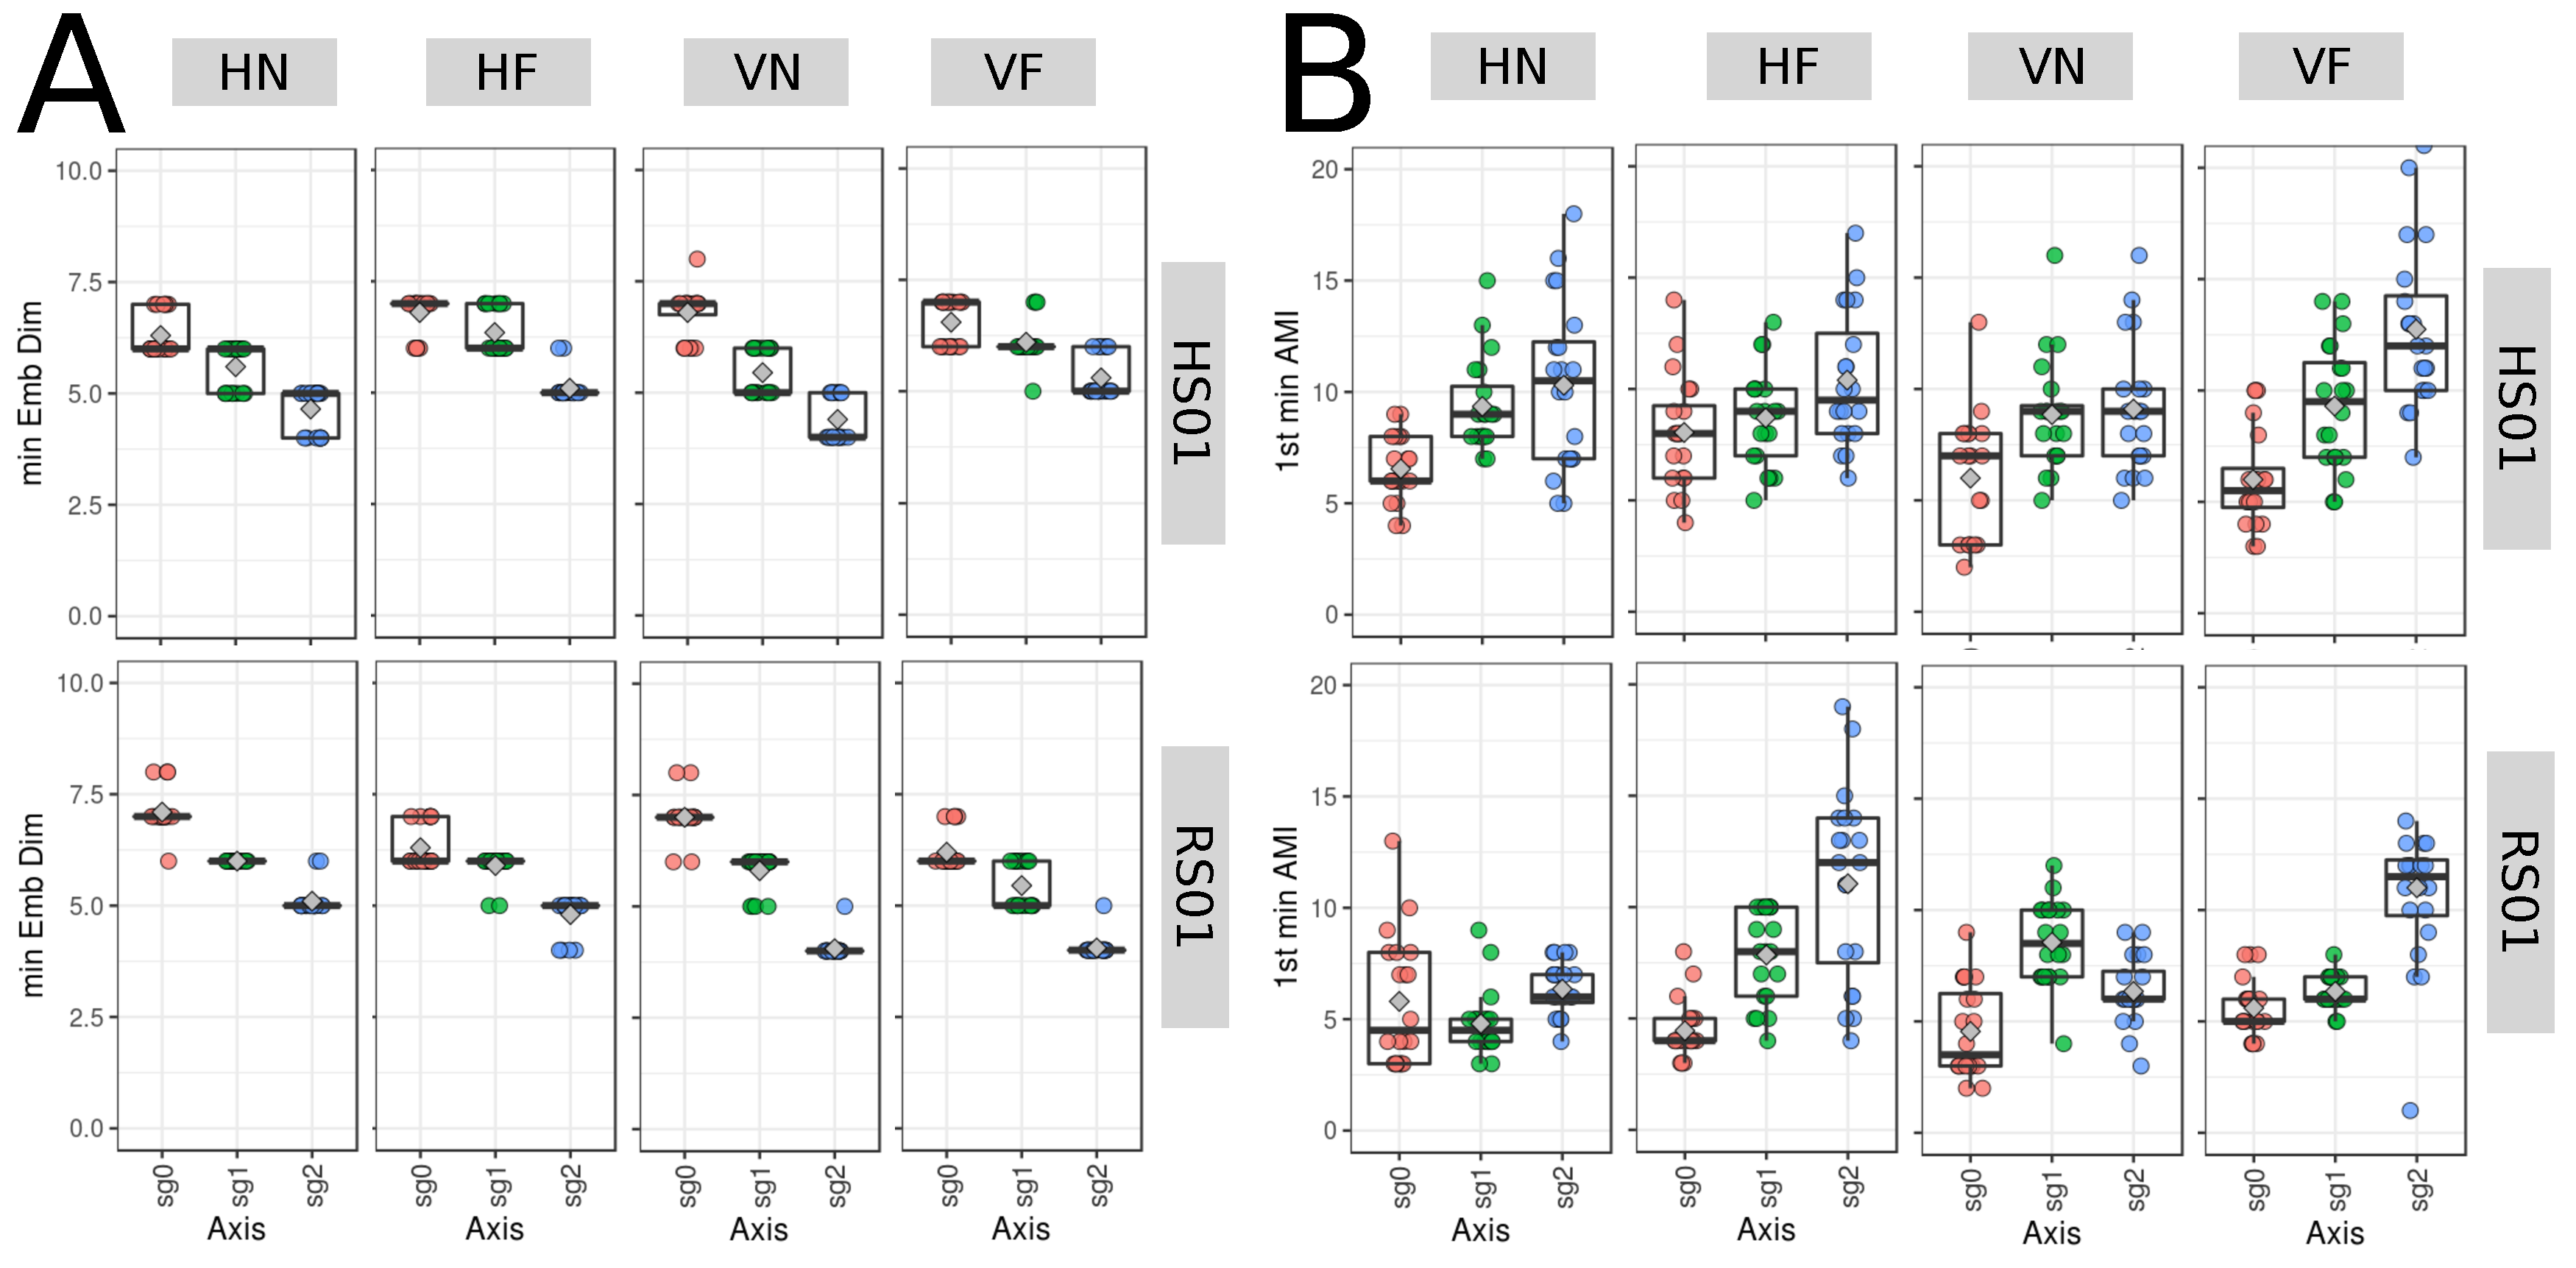
\includegraphics[width=1.0\textwidth]{fig-fig2.pdf}
	\caption{
	{\bf Box plots of minimum embedding parameters.} 
	Box plots of (A) minimum embedding dimensions 
	and (B) first minimum AMI values for 
	Horizontal Normal (HN), Horizontal Faster (HF),
	Vertical Normal (VN) and Vertical Faster (VF)
	with sensors attached to participants (HS01) and
	sensor attached to robot (RS01).
	Minimum embedding parameters are for twenty participants 
	($p01$ to $p20$) with three smoothed signals 
	(sg0: sg0zmuvGyroZ, sg1: sg1zmuvGyroZ and sg2: sg2zmuvGyroZ)
	and window length of 10-sec (500 samples).
	Code and data to reproduce the figure is available in \cite{srep2020}.
        }
    \label{fig:cao_ami}
\end{figure}
%%---------------------------------(FIGURE)------------------------------------

\subsubsection*{Uniform Time-Delay Embedding}
Using the overall embedding parameters ($\overline{m_0}=6$, $\overline{\tau_0}=8$), 
the first three axis of the rotated Principal Components Analysis (PCA) 
are shown for the reconstructed state spaces of horizontal (figures~\ref{fig:rsss}(A)) 
and vertical (figures~\ref{fig:rsss}(B)) arm movements. 
While visual inspection of these figures 
suggests differences in the trajectories of the reconstructed state spaces, 
we require an objective quantification to determine the extent of the differences.  
One approach could be use Euclidean distances from the origin for points in these 
trajectories, but this proved inconclusive and was not able to capture 
the dynamics of the trajectories. Consequently, we applied 
Recurrence Plots and Recurrence Quantification Analysis.
%%---------------------------------(FIGURE)-------------------------------------
\begin{figure}[ht]
\centering
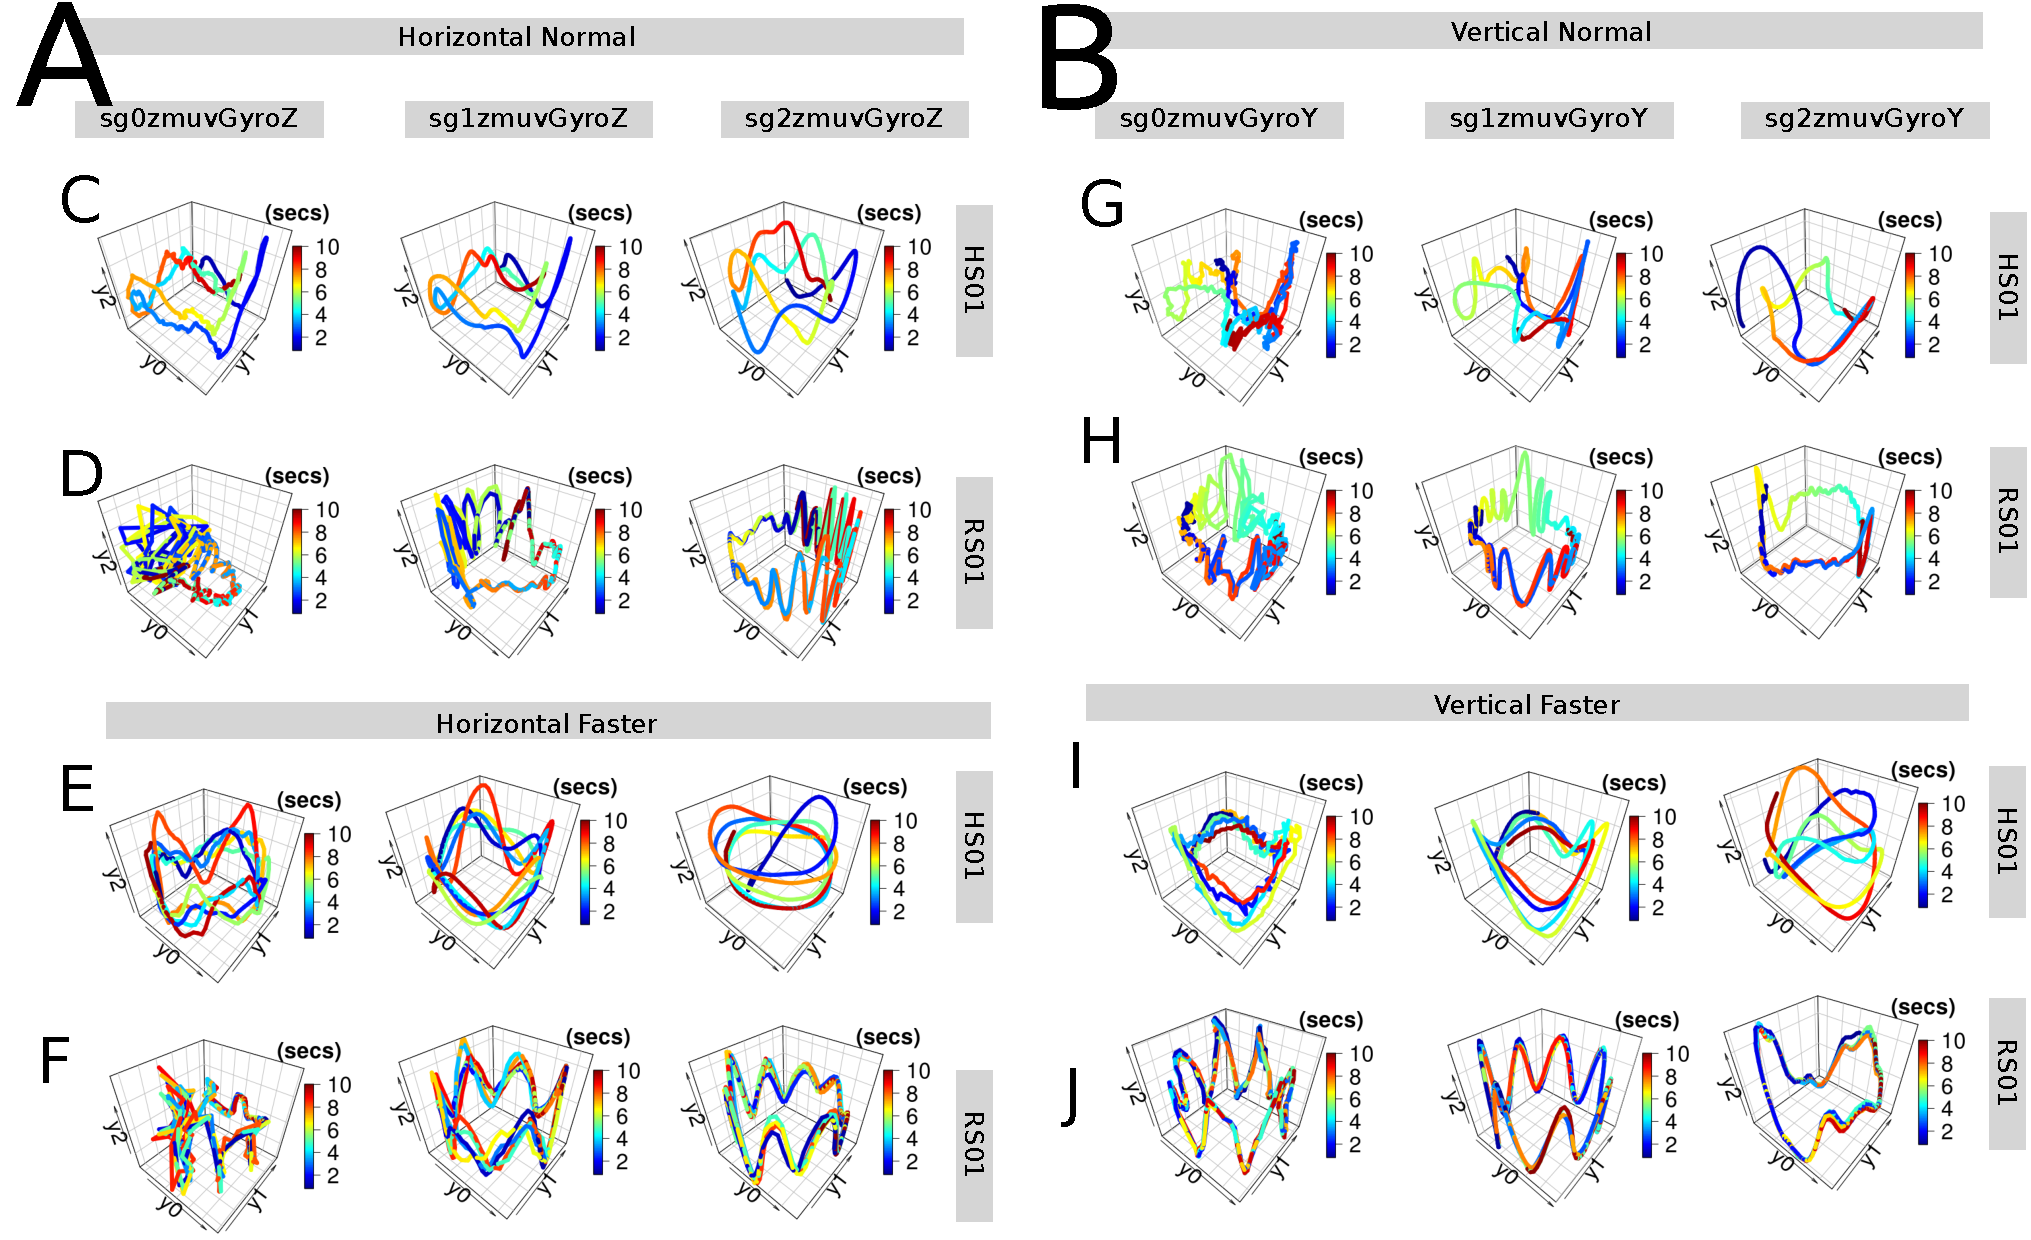
\includegraphics[width=1.0\textwidth]{fig-fig3.pdf}
\caption{
	{\bf RSSs for horizontal and vertical arm movements.}
	Reconstructed state spaces for time series for p01 of Figure \ref{fig:ts}.
	Reconstructed state spaces were computed with 
	embedding parameters 
	$\overline{m}_0=6$, $\overline{\tau}_0=8$
	for (A) horizontal and (B) vertical arm movements.
	Code and data to reproduce the figure is available in \cite{srep2020}.	
        }
    \label{fig:rsss}
\end{figure}
%%---------------------------------(FIGURE)------------------------------------



\subsection*{Recurrences Plots}
Using the average embedding parameters 
($\overline{m}_0=6$, $\overline{\tau}_0=8$) 
and an recurrence threshold of $\epsilon=1$.
As our interest is for dynamical transitions, 
there is little importance on the selection of $\epsilon$ which in this case
is 1. 
Recurrence Plots (RP) were computed for horizontal (figures~\ref{fig:rps}(A)) and 
vertical (figures~\ref{fig:rps}(B)) arm movements.
%%---------------------------------(FIGURE)-------------------------------------
\begin{figure}[ht]
\centering
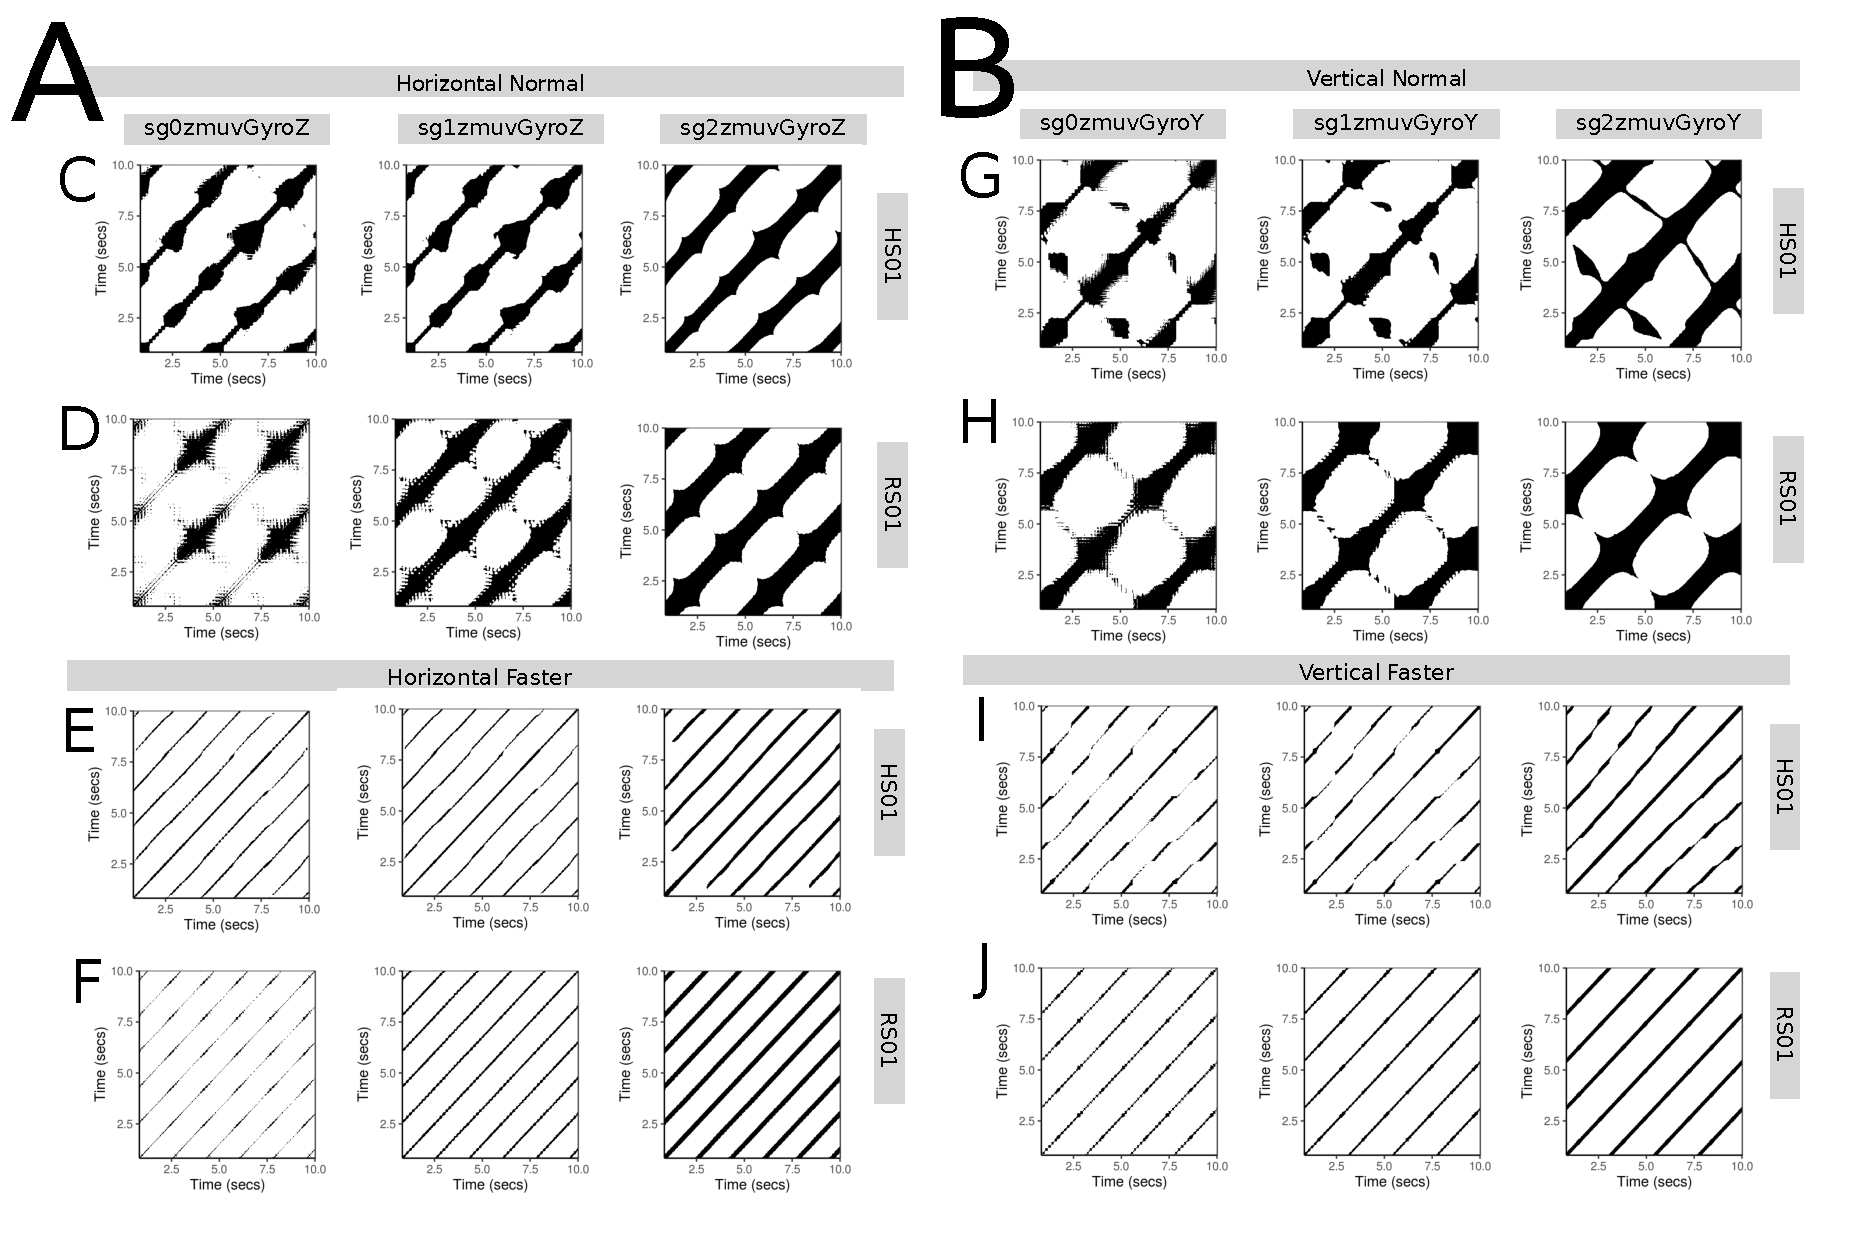
\includegraphics[width=1.0\textwidth]{fig-fig4.pdf}
\caption{
	{\bf RPs for horizontal (A) and vertical (B) arm movements.}	
	Recurrence plots were computed with 
	embedding parameters 
	$\overline{m}_0=6$, $\overline{\tau}_0=8$, and $\epsilon=1$.
	Code and data to reproduce the figure is available in \cite{srep2020}.
        }
    \label{fig:rps}
\end{figure}
%%---------------------------------(FIGURE)------------------------------------

\subsection*{Recurrence Quantification Analysis} \label{ch6:rqas}
Four Recurrence Quantification Analysis metrics (
percentage recurrence, REC, representing the percentage of black dots in RP; 
percentage determinism, DET, representing the predictability of the RP; 
ratio of DET / REC, RATIO; Shannon entropy, ENTR) 
were computed using the same parameters as for RP.
%\subsubsection*{REC values}
Figure~\ref{fig:RQABP}(A) presents box plots of REC values, 
for HS01, are more spread for Slow (i.e., 5 seconds per movement) movements 
in Horizontal (HS) or Vertical (VS) than for Fast (i.e., 2 seconds per movement).  
This suggests greater variation between participants for the Slow movements.  
For RS01, there is little variation between Slow and Fast movement
(interquartile range of 0.01). 
In terms of smoothness, there seems little effect of HS01 but RS01 values 
do show affects of smoothness (see the incremental changes of mean values (rhombus)).
%\subsubsection*{DET values}
Figure \ref{fig:RQABP}(B) presents DET values and shows 
little difference for type of movement or performer.  
However, DET values are affected by changes in smoothness of the signal, 
particularly for Fast movement.
%\subsubsection*{RATIO values}
Figure \ref{fig:RQABP}(C) presents the ratio of DET / REC. 
These values, for the human performer, vary less for HN than for HF movement.  
Additionally, smoothness leads to a decrease in mean values for Fast movements.
%\subsubsection*{ENTR values}
Figure \ref{fig:RQABP}(D) shows ENTR values are higher for the human 
performer than the robot, and vary with the smoothness of the time-series.
%%---------------------------------(FIGURE)-------------------------------------
\begin{figure}
\centering
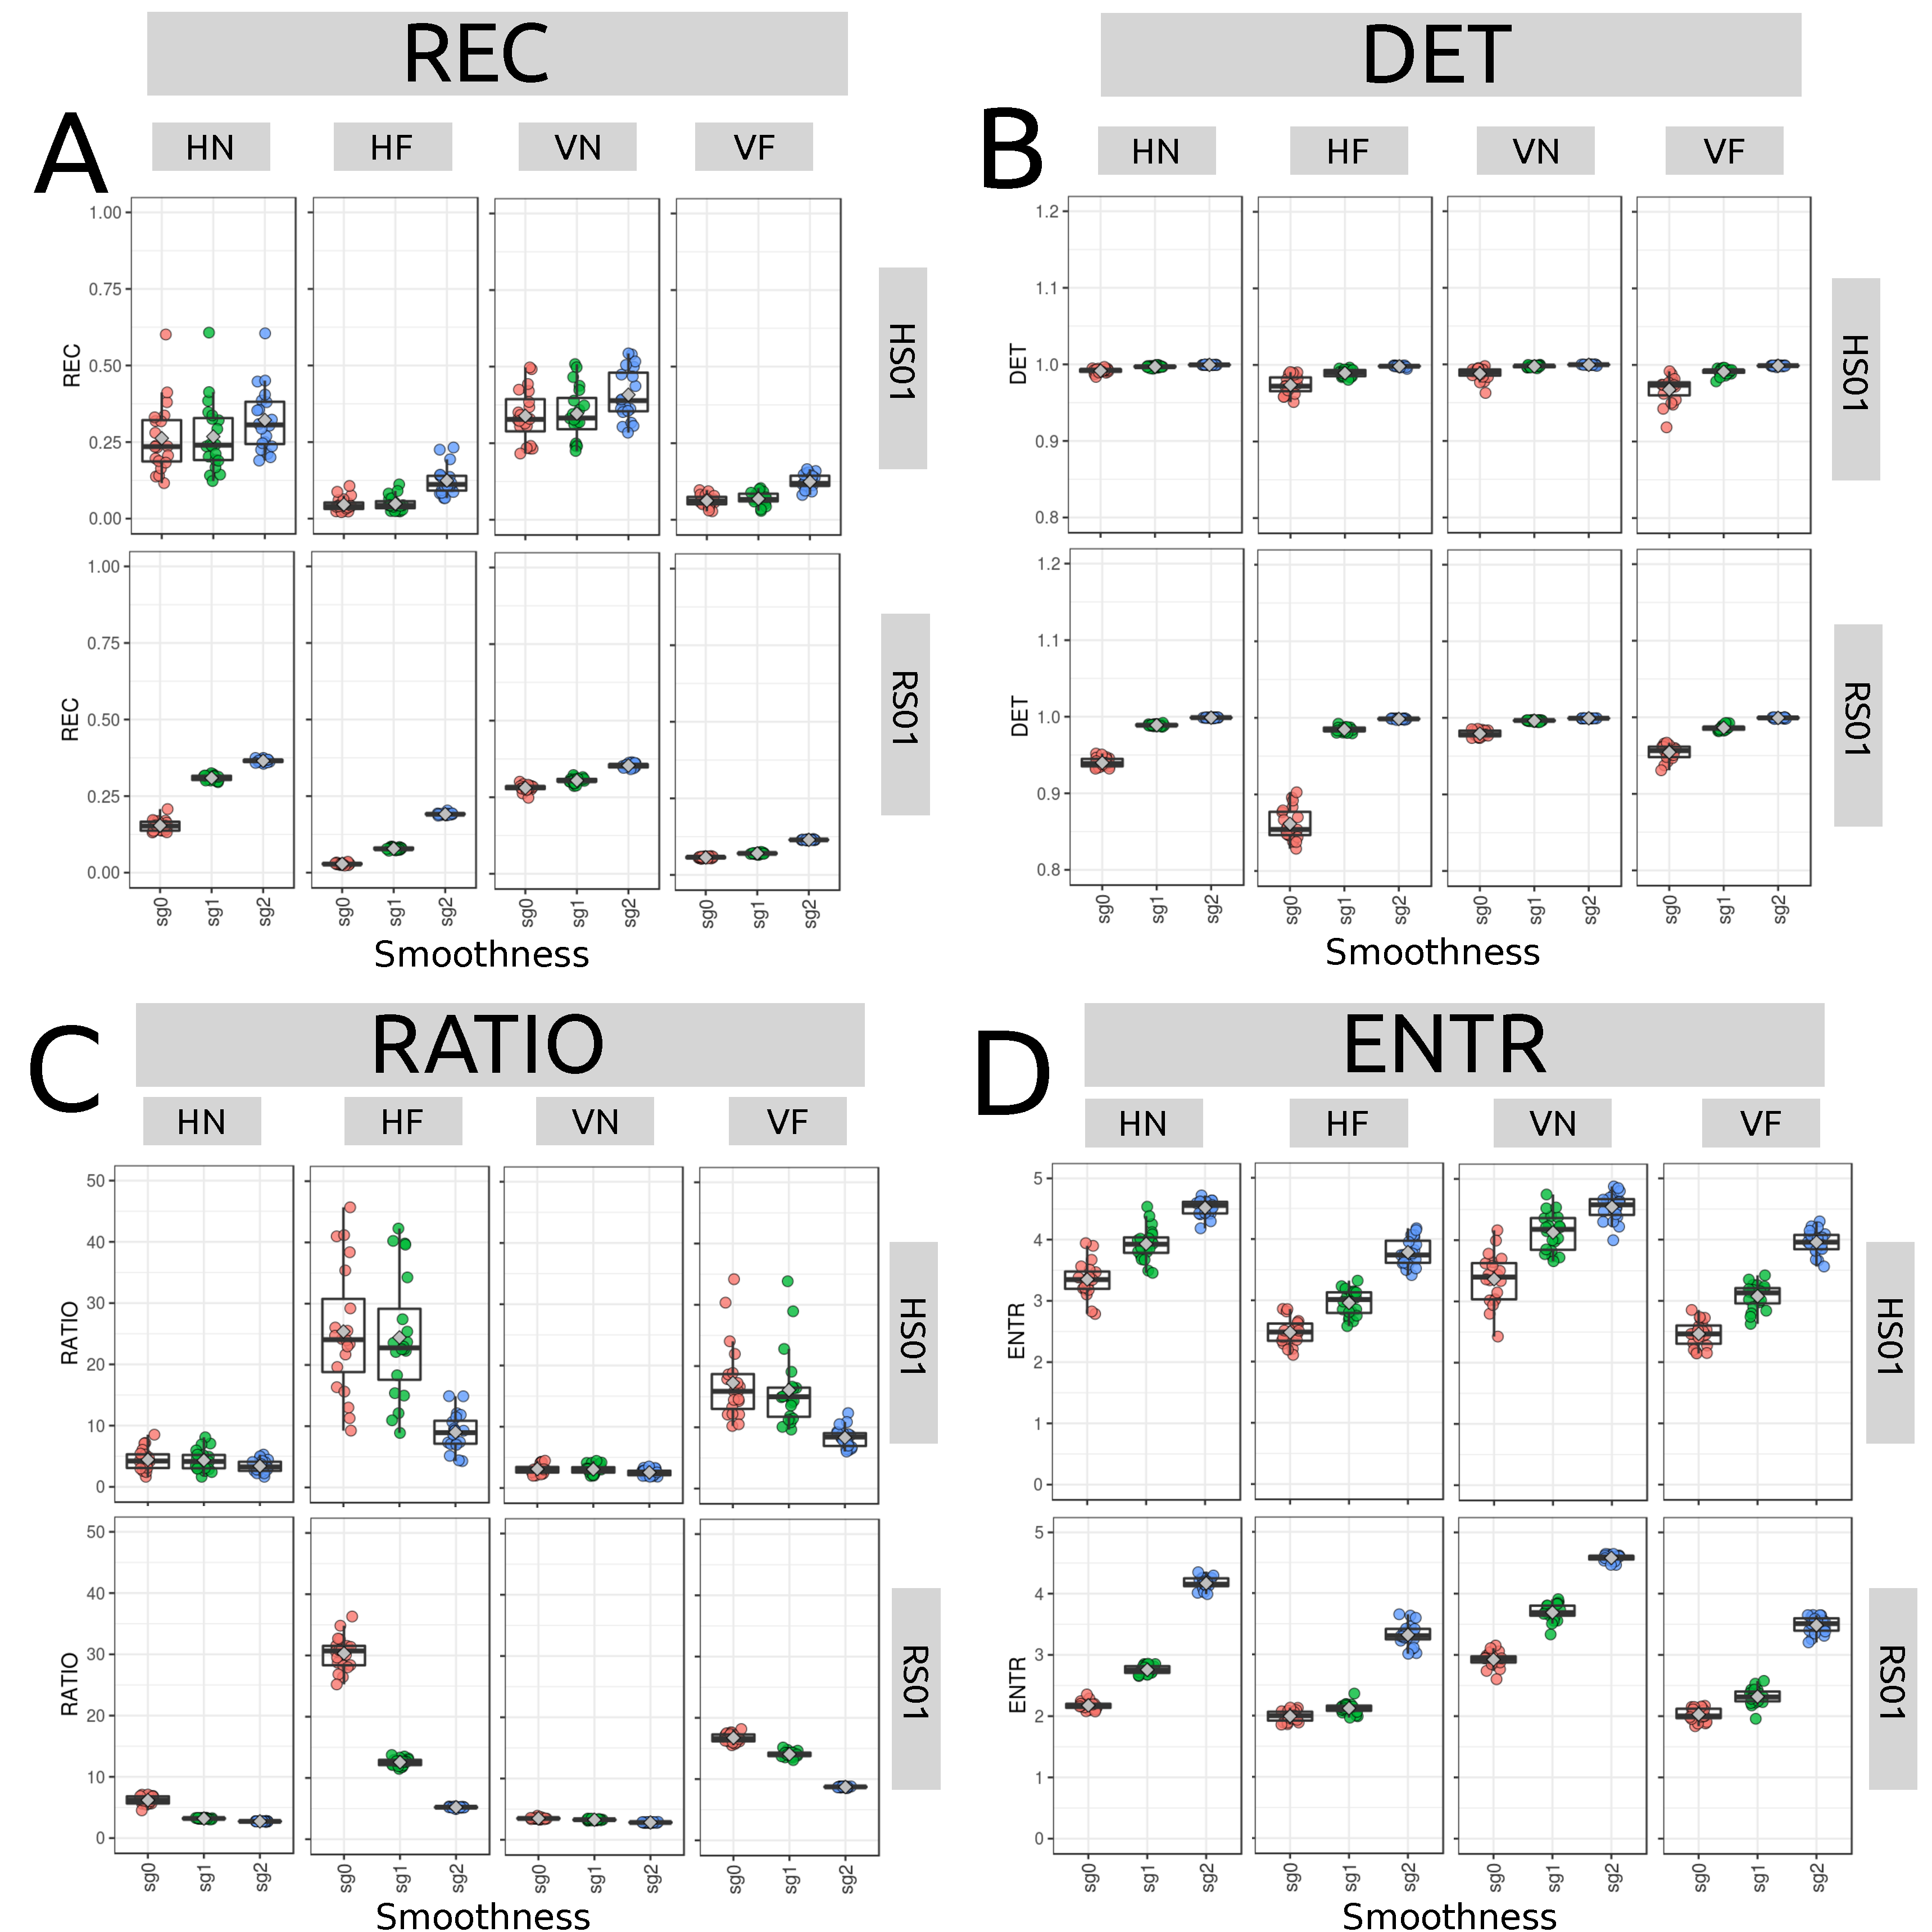
\includegraphics[width=1.0\textwidth]{fig-fig5.pdf}
    \caption
	[Box plots for RQA values]{
	{\bf Box plots for RQA metrics.}
	RQA metrics for (A) REC, (B) DET, (C) RATIO, and (D) ENTR of 
	20 participants performing HN, HF, VN and VF movements
	with sensors HS01, RS01 and three smoothed-normalised  
	time series (sg0, sg1 and sg2).
	RQA values were computed with 
	$\overline{m}_0=6$, $\overline{\tau}_0=8$, and $\epsilon=1$. 
	Code and data to reproduce the figure is available in \cite{srep2020}.
        }
    \label{fig:RQABP}
\end{figure}
%%---------------------------------(FIGURE)------------------------------------

%\subsection*{RQA metrics with fixed parameters}
%Considering that RQA metrics were computed with fixed embedding parameters 
%($m=6$ and $\tau=8$) and recurrence thresholds ($\epsilon=1$), we found 
%the following. REC values, which represents the \% of black points in the RPs, 
%were more affected with and increase in normal speed movements (HN and VN) 
%than faster movements (HF and VF) for the sensor attached to the participants 
%(HS01). Such decrease of REC values from normal speed to faster speed 
%movements is also presented in data from sensor attached to the robot (RS01), 
%and little can be said with regard to the dynamics of the time series coming 
%from RS01 (Fig \ref{fig:RQABP}A).
%Similarly, DET values, representing predictability and 
%organisation in the RPs, present little variation in the any of the time 
%series where little can be said (Fig \ref{fig:RQABP}B).
%In contrast, RATIO values, which represent 
%dynamic transitions, were more variable for faster movements (HF and VF) 
%than normal speed movements (HN and VN) with sensors attached to the 
%participants (HS01). For data coming from sensors attached to the robot 
%(RS01), RATIO values from horizontal movements (HN, HF) appear to vary 
%more than values coming from vertical movmentes (VN, VF) 
%(Fig \ref{fig:RQABP}C).
%With that, it can be said that RATIO values can represent a bit better
%than REC or DET metrics for the variability of imitation activities in 
%each of the conditions for time series.
%Similarly, ENTR values for HN were higher than values for HF
%and ENTR values varied more for sensor attached to participants 
%than ENTR values for sensors of the robot. It is evidently that 
%the higher the entropy the more complex the dynamics are, 
%however, ENTR values for HN appear a bit higher than HF values, 
%for which we believe this happens because of the structure the time series
%which appear more complex for HN than  HF movements which presented a 
%more consistence repetition (Fig \ref{fig:RQABP}D).


\subsection*{3D RQA ENTR}
As ENTR appeared to be have higher sensitivity than the other measures, 
we explored the impact of different embedding parameters 
$ \{ m \in \mathbb{R} | 1 \le m \le 10  \} $,
$  \{ \tau \in \mathbb{R} | 1 \le \tau \le 10  \} $ 
incrementing by 1 each run, with recurrence thresholds $\epsilon=1, 2, 3$ 
and levels of smoothness (sg0, sg1, sg2).  
Figure \ref{fig:RQA-IND} shows that increasing recurrence 
threshold leads to an increase in ENTR regardless of level of smoothness.  
Similarly, increasing level of smoothness will also increase ENTR (figure \ref{fig:RQA-IND}).
In terms of movement or performer, RQA ENTR decrease from Slow (HS, VS) to Fast (HF, VF) 
for both human (HS01) and (RS01) (Figures~\ref{fig:3dRQAENTR_sensoractivities}).
In terms of individual differences, for human participants, 
figure \ref{fig:3dRQAENTR_participantsactivities} compares p01, p02 and p03 (for illustrative purposes) --
both between each other and in comparison with the more consistent performance of the robot.  
In terms of window length (w100 (2s), w250 (5s), w500(10s), w750 (15s)), 
figure \ref{fig:3dRQAENTR_windowsactivities} shows that improvement in 
capture with number of samples, although this has less of an effect on RQA ENTR.

%%---------------------------------(FIGURE)-------------------------------------
\begin{figure}
\centering
\includegraphics[width=1.0\textwidth]{fig-rqa-epsilons.pdf}
    \caption
	[3D surface plots of RQA ENTR values]{
	{\bf 
	3D surface plots of RQA ENTR values for different recurrence threshold and smoothness levels.}
	RQA ENTR values are
	for embedding parameters
	$ \{ m \in \mathbb{R} | 0 \le m \le 10  \} $,
	$ \{ \tau \in \mathbb{R} | 0 \le \tau \le 10  \} $
	incrementing by one and three recurrence thresholds $\epsilon=1, 2, 3$.
	RQA ENTR values were computed with data from $p03$, sensor HS01, with 
	a window size of 10-secs (500 samples).
	Code and data to reproduce the figure is available in \cite{srep2020}.
        }
    \label{fig:RQA-IND}
\end{figure}
%%---------------------------------(FIGURE)------------------------------------

%%---------------------------------(FIGURE)-------------------------------------
\begin{figure}[ht]
\centering
\includegraphics[width=1.0\textwidth]{fig-rqa-sensors-activities.pdf}
    \caption{
	{\bf 3D surface plots of RQA ENTR values for different sensors and activities.}
	RQA ENTR values are for embedding parameters
	$ \{ m \in \mathbb{R} | 0 \le m \le 10  \}$,
	$ \{ \tau \in \mathbb{R} | 0 \le \tau \le 10  \}$
	with $\epsilon = 1 $ considering four activities 
	Horizontal Normal (HN), Horizontal Faster(HF), Vertical Normal(VN), and 
	Vertical Faster (VF) and sensors Human Sensor 01 (HS01) and 
	Robot Sensor (RS01).
	RQA ENTR values were computed from data of $p03$, sg0 and 
	window size of 10-secs (500 samples).
	Code and data to reproduce the figure is available in \cite{srep2020}.
       }
\label{fig:3dRQAENTR_sensoractivities}
\end{figure}
%%---------------------------------(FIGURE)-------------------------------------

%%---------------------------------(FIGURE)-------------------------------------
\begin{figure}[ht]
\centering
\includegraphics[width=0.9\textwidth]{fig-rqa-participants.pdf}
    \caption{
	{\bf 3D surface plots of RQA ENTR values for different participants, activities and sensors.}
	RQA ENTR values are for participants (p01, p02, and p03) 
	in the categories of 
	(A) Human Sensor 01 (HS01) and 
	(B) Robot Sensor 01 (RS01)
	considering embedding parameters
	$ \{ m \in \mathbb{R} | 0 \le m \le 10  \}$,
	$ \{ \tau \in \mathbb{R} | 0 \le \tau \le 10  \}$
	with $\epsilon = 1$ and four activities 
	Horizontal Normal (HN), Horizontal Faster(HF), Vertical Normal(VN), and 
	Vertical Faster (VF).
	RQA ENTR values were computed from data of sg0 and window size of 10-secs (500 samples).
	Code and data to reproduce the figure is available in \cite{srep2020}.
       }
\label{fig:3dRQAENTR_participantsactivities}
\end{figure}
%%---------------------------------(FIGURE)-------------------------------------

%%---------------------------------(FIGURE)-------------------------------------
\begin{figure}[ht]
\centering
\includegraphics[width=1.0\textwidth]{fig-rqa-windows}
    \caption{
	{\bf 3D surface plots of RQA ENTR values for different windows lengths and activities.}
	RQA ENTR values are for embedding parameters
	$ \{ m \in \mathbb{R} | 0 \le m \le 10  \}$,
	$ \{ \tau \in \mathbb{R} | 0 \le \tau \le 10  \}$, 
	with $\epsilon = 1 $ considering four 
	windows lengths (e.g., w100 (100 samples), w250 (250 samples),
	w500 (500 samples) and w750 (750 samples)) and
	four activities 
	Horizontal Normal (HN), Horizontal Faster(HF), Vertical Normal(VN), and 
	Vertical Faster (VF).
	RQA ENTR values were computed from data of $p01$ and sg0.
	Code and data to reproduce the figure is available in \cite{srep2020}.
       }
\label{fig:3dRQAENTR_windowsactivities}
\end{figure}
%%---------------------------------(FIGURE)-------------------------------------

To summarise this section of results, it can be said that computing
embedding parameters for individual structure of time-series 
data is already a solved problem \cite{frank2010, sama2013, bradley2015}. 
However, it has been shown the challenge of finding embedding parameters
for nonlinear dynamic tools that represent a set of different time-series data.
That said, we proposed the use of sample mean of the set of embedding parameters
for RSSs, RP and RQA to then noticed that the selection of recurrence 
threshold, $\epsilon$, is also an open problem.
For which, this work proposed the variation of recurrence thresholds 
and embedding parameters to show the relationships of these to different datasets 
(participants, activities, windows lengths and sensors).

%*******************************************************************************
%*******************************************************************************
%*******************************************************************************
\section*{Discussion}
While there are many approaches to estimating embedding parameters for nonlinear analysis, 
these can be influenced by the structure of the time-series data.   
We show that, for RSS, RP and RQA, the estimation of embedding parameters can be performed 
using a sample mean which, together with recurrence threshold, can be shown to be 
influenced by activity, performer, window length and smoothness of time-series.  
It is known that time-series from different sources and with different characteristics 
require different embedding parameters, and this can produce different RSS, RPs and RQAs. 
Although this work helps to understand the open problem of 
finding right balance among (i) the level of smoothness of the signal, 
(ii) the selection of recurrence thresholds and (iii) 
the range of embedding parameters, 
we have shown how RQA metrics can help to quantify movement variability.

\section*{Conclusions}
In this paper we show how the selection of nonlinear analysis tool  
(i.e., RSS, RP, RQA metrics) depends on what question one wishes to 
address with time-series data (e.g., predictability, organisation, dynamics, complexity).  
Time-series data characteristics (e.g., window length, smoothness), 
time-series structure (e.g., frequency, amplitude) and 
data source (e.g., sensor placement, performance, movement) all influence 
the results that nonlinear analysis methods can provide.
That said, it has been shown that the use of different characteristics of the data and 
their collection can help us visualise and quantify variability of movement using 
methods of nonlinear analysis.   
There remain limitations of nonlinear methods in 
relation to the estimation of parameters (e.g., recurrence threshold, embedding parameters) 
which reflect the dynamics of specific movement and performers, window length 
and structure of the time-series. 
We note that RQA DET seems to show low sensitivity 
to these differences, whereas REC and RATIO (primarily as a result of REC) show 
variation across performers and movements.   
RQA ENTR, with different recurrence thresholds, 
can quantify variation in the time-series data and offers the most appropriate means 
for analysing variability in movement to allow us to analyse individual differences 
between human performers.  
To then found out that RQA ENTR values with different recurrence 
thresholds were appropriate to quantify 
the different changes and variations of the characteristics of 
time-series data.
Therefore, the use of Shannon Entropy could be applied 
to analyse human participants who might vary in age, 
state of health, anthropometric features and capability to perform movement.

%% As a guideline references should be limited to 60 (this is not 
%% strictly enforced).
%\bibliography{sample}
%\bibliography{../references/references}
%\bibliography{references}
%*******************************************************************************
\documentclass[fleqn,10pt]{wlscirep}
\usepackage[utf8]{inputenc}
\usepackage[T1]{fontenc}
%\graphicspath{{../}} %goes to path: docs/

\title{Nonlinear methods to quantify Movement Variability in Human-Humanoid Interaction Activities}
\author[1,*]{Miguel Xochicale}
\author[2]{Chris Baber}
\affil[1]{King's College London, 
	School of Biomedical Engineering amd Imaging Sciences,
	London, SE1 7EU, UK
	} 
\affil[2]{University of Birmingham,
	School of Computer Science,
	Birmingham, 
	B15 2TT, 
	UK}
\affil[*]{miguel.xochicale@kcl.ac.uk}


%\keywords{Keyword1, Keyword2, Keyword3}

\begin{abstract}
Human movement variability arises from the process of 
mastering redundant (bio)mechanical degrees of freedom (DOF)
to successfully accomplish any given motor task
(from the most complex to even the simplest one) 
where flexibility and stability of many possible joint 
combinations helps to adapt to environment conditions. 
While the analysis of movement of variability is becoming increasingly 
popular as a diagnostic tool or skill performance evaluation, 
there are remain challenges in terms of defining 
the most appropriate methods and parameters to apply. 
For this work, we therefore investigate nonlinear dynamics methods 
such as reconstructed state space (RSSs), uniform time-delay embedding, 
recurrence plots (RPs) and recurrence quantification analysis metrics (RQAs)
with real-world time-series data of wearable inertial sensors. 
That said, twenty right-handed healthy participants 
imitated simple vertical and horizontal arm movements in normal 
and faster velocity from an humanoid robot.
We applied nonlinear methods to four activities, 
four window lengths and three levels of smoothed time-series data,
to then found visual differences in the patterns of RSSs and RPs
and statistical differences with RQA metrics.
We therefore conclude that Shannon Entropy for RQA is a robust method 
that help us to quantify activities, types of sensors, windows lengths 
and level of smoothness.
Hence this work might enhance the development of 
better diagnostic tools for applications in 
rehabilitation and sport science for skill performance
or new forms of human-humanoid interaction for
quantification of movement adaptations and motor pathologies.
\end{abstract}


\begin{document}
\flushbottom
\maketitle
\thispagestyle{empty}

\section*{Introduction}
The complexity of human movement arises from the process of mastering 
redundant (bio)mechanical degrees of freedom (DOF) to successfully 
accomplish any given motor task (Bernstein, 1967).
Such DOF are independent coordinates to uniquely 
describe the configurations of the system which provides flexibility 
and stability to adapt to a change environment conditions but 
that leads many possible combinations (Newell and Vaillancourt, 2001).
Hence, human movement complexity can be seen as a balance 
between the required DOF "to generate a stable (persistent) 
and flexible (variable) behavioural output in response to 
changing intentions and dynamic environmental
conditions" \cite{davids2003}. 
Consequently, one can see much variability in human movement even in the 
simplest of movements.  
While the analysis of movement of variability is becoming increasingly 
popular as a diagnostic tool or skill performance evaluation, 
there remain challenges in terms of defining 
the most appropriate methods and parameters to apply. 
In part, 
these challenges stem from the fact that the identification movement 
variability requires analysis of signals which are time-series of 
of $1-$dimension in $\mathbb{R}$ which are 
noisy, nonlinear and non-stationary \cite{gomezgarcia2014}.
Further problems arise from assigning a plausible locus of control to 
the movements, e.g., in order to determine whether variability is the 
result of deliberative control by the performer or whether it arises 
from exogenous or endogenous disturbances.  For this paper, our focus 
is on the analysis of signals; specifically, in terms of objectively 
quantifying variability of lower dimension signals using time-series analysis.

Methods for nonlinear time series analysis generally involve the estimation of the 
embedding parameters ($m$ embedding dimension and $\tau$ embedding delay) to 
reconstruct the state space,
where an $n$-dimensional is reconstructed state space using $1-$dimensional 
time series \cite{Quintana-Duque2012, Quintana-Duque2016, sama2013, 
frank2010, gomezgarcia2014, marwan2011, stergiou2011}.
Key to the selection of these parameters is the need to preserve 
topological properties of an unknown $M$-dimensional state space \cite{takens1981}.
An common approach to the construction of these state spaces 
involves Recurrence Plots (RPs), a graphical representation of black and white dots, 
which shows recurrent patterns of a $n$-dimensional system.
While RPs provide a human
interpretable picture of the system, these require further
analysis to allow the properties of that system to be quantified,
and so Recurrence Quantification Analysis (RQA) can be applied.
However, the estimation of the embedding parameters for
RQA remains an open problem (Bradley et al. 2015 \cite{bradley2015})
There is no agreed method to estimate embedding parameters
for RQA and other nonlinear methods \cite{bradley2015} 
because time series are system-dependent, i.e., these rely
on the initial conditions, and on the configuration and behaviour of the system.  
This means that, unless one holds all of the influencing 
variables constant, embedding parameters computed for one 
instance may not apply to another instance.   

One could apply methods, such as autocorrelation, mutual information, 
nearest neighbour (and we will apply these in this paper), 
but these methods assume that the data are well sampled, with 
little noise and (usually) that the signals are purely deterministic \cite{garland2016, kantz2003}.
That said, these methods can break-down in the face of real-world datasets 
which could have 
different length, 
different values of accuracy and precision (rounding errors due to finite 
precision of the measurement apparatus which include frequency 
acquisition \cite{frank2010}), or 
different levels of contamination from exogenous and endogenous 
sources of ‘noise’ \cite{garland2016}.  What is, perhaps, surprising is that 
even subject to these problems, the methods are useful and 
nonlinear dynamics approaches continue to tell us much about 
human movement \cite{Quintana-Duque2012, Quintana-Duque2016, sama2013, frank2010,
gomezgarcia2014, marwan2011, stergiou2011, bradley2015}.

For this paper, we explore the role of RPs and RQA in the 
analysis of simple human movement. 
We compare horizontal and 
vertical arm movements performed by neurotypical participants 
who are copying these movements being made by a humanoid robot.  
This provides an initial point of comparison 
(between human movement, which we assume to have a degree of variability, 
and the robot, which we assume to have a degree of consistency).   
Additionally, our interest lies in the estimation of embedding parameters 
in light of different features of the data, e.g., levels of smoothing, 
window length, structure of time-series based on movement, 
types of sensors, individual differences between participants and 
the movements that they perform. 
Specifically, we ask what are 
the effects of different embedding parameters, recurrence thresholds 
and characteristics of time-series on nonlinear analysis 
methods (i.e., reconstructed state space with 
uniform time-delay embedding, RPs and RQA)?



%*******************************************************************************
%*******************************************************************************
%*******************************************************************************
\section*{Methods}
\subsection*{State Space Reconstruction}
The method of state space reconstruction \cite{packard1980} 
\cite{takens1981} has been applied in many disciplines 
\cite{aguirre2009, stergiou2011, frank2010, 
sama2013, Quintana-Duque2016}. The method of state space reconstruction is 
based on uniform time-delay embedding methodology which is a simple 
matrix implementation that can reconstruct an unknown $d-$dimensional 
manifold $M$ from a scalar time series (e.g. one-dimensional 
time series in $\mathbb{R}$). A manifold, in this context, is a 
multidimensional curved surface within a space (e.g. a saddle) 
\cite{guastello-gregson2011}.

The use of a scalar time series is the main advantage of the method of state 
space reconstruction which in essence preserve dynamic invariants such as 
correlation dimension, fractal dimension, Lyapunov exponents, Kolmogorov-Sinai 
entropy and detrended fluctuation analysis \cite{bradley2015, 
Quintana-Duque2012, Quintana-Duque2013, Quintana-Duque2016, krakovska2015}.
However, selecting appropriate embedding parameters which are sued to apply the 
state space reconstruction is still an open challenge for which we present 
introductions for the methodologies to compute such embedding parameters 
With that in mind, in the following subsections, we describe in more detail 
the state space reconstruction theorem (RSSs), uniform time-delay embedding 
theorem (UTDE), false nearest neighbours (FNN) and average mutual 
information (AMI). 
%and other methodologies for state space reconstruction.

\subsection*{State Space Reconstruction Theorem}
Following the notation employed in \cite{casdagli1991, garland2016, gibson1992,
uzal2011, uzal2010, takens1981}, state space reconstruction is defined by:
%%********************************[EQUATION]************************************
\begin{equation}\label{eq:ssr}
  s(t)=f^t [s(0)],
\end{equation}
%%********************************[EQUATION]************************************
where $s$, $s: A \rightarrow M$ given that $A \subseteq \mathbb{R}$ and 
$M \subseteq \mathbb{R}^d$, represents a trajectory which evolves in an 
unknown $d-$dimensional manifold $M$, $f: M \rightarrow M$ is an evolution 
function and $f^t$, with time evolution $t \in \mathbb{N}$, is the $t$-th 
iteration of $f$ that corresponds to an initial position 
$s(0) \in M $ \cite{takens1981}.
%$f$ is a smooth dynamical system, where smooth means a 
%continuously differentiable system
%(e.g. derivatives exist at all points) \cite{guastello-gregson2011}.
Then, a point of a one-dimensional time series $x(t)$ in $\mathbb{R}$, 
can be obtained with
%%********************************[EQUATION]************************************
\begin{equation}\label{eq:measurement}
  x(t)=h[s(t)],
\end{equation}
%%********************************[EQUATION]************************************
where $h$ is a function, $h: M \rightarrow \mathbb{R}$, defined on the trajectory $s(t)$.
Reconstructed state space can then be described as an $n-$dimensional state 
space defined by $y(t)=\Psi[\boldsymbol{X}(t)]$ where 
$\boldsymbol{X}(t) = \{ x(t), x(t-\tau) , ...,x(t - (m-1)\tau  ) \}$ 
is the uniform time-delay embedding with a dimension embedding $m$
and delay embedding $\tau$ and
$ \Psi: \mathbb{R}^m \rightarrow \mathbb{R}^n$ is a further transformation
of dimensionality (e.g. Principal Component Analysis, 
Singular Value Decomposition, etc) being $n \leq m$.
With that in mind, uniform time-delay embedding, $\boldsymbol{X}(t)$, 
defines a map $\Phi: M \rightarrow \mathbb{R}^m$ such that 
$\boldsymbol{X}(t) = \Phi(s(t))$,
where $\Phi$ is a diffeomorphic map \cite{takens1981}
whenever $\tau > 0$ and $m > 2d_{box}$ and $d_{box}$ is the box-counting
dimension of $M$ \cite{garland2016}.
% "Given two manifolds $M$ and $N$, a differientiable map $f: M \rightarrow N$
% is called diffeomorphic if it is one-to-one correspondence and its inverse
% $f^{-1}: N \rightarrow M$ is differientiable as well \cite{wiki:diffeomorphic}".
Then, if $\Phi$ is an embedding of evolving trajectories in the reconstructed 
space then a composition of functions represented with $F^t$ is induced on the
reconstructed state space determined:
%by true smooth dynamical system $f^t$ and $\Phi$:
%********************************[EQUATION]************************************
\begin{equation}\label{eq:st}
  \boldsymbol{X}(t)=F^t [\boldsymbol{X}(0)] = \Phi \circ f^t \circ \Phi ^{-1}[\boldsymbol{X}(0)].
\end{equation}
%%********************************[EQUATION]************************************
With this in mind, an embedding is defined as "a smooth one-to-one 
coordinate transformation with a smooth inverse" and the total reconstruction 
map is defined as $ \Xi = \Psi \circ \Phi $ \cite{casdagli1991}.
Fig~\ref{fig:ssr} illustrates the state space reconstruction.
%%---------------------------------(FIGURE)-------------------------------------
\begin{figure}[ht]
\centering
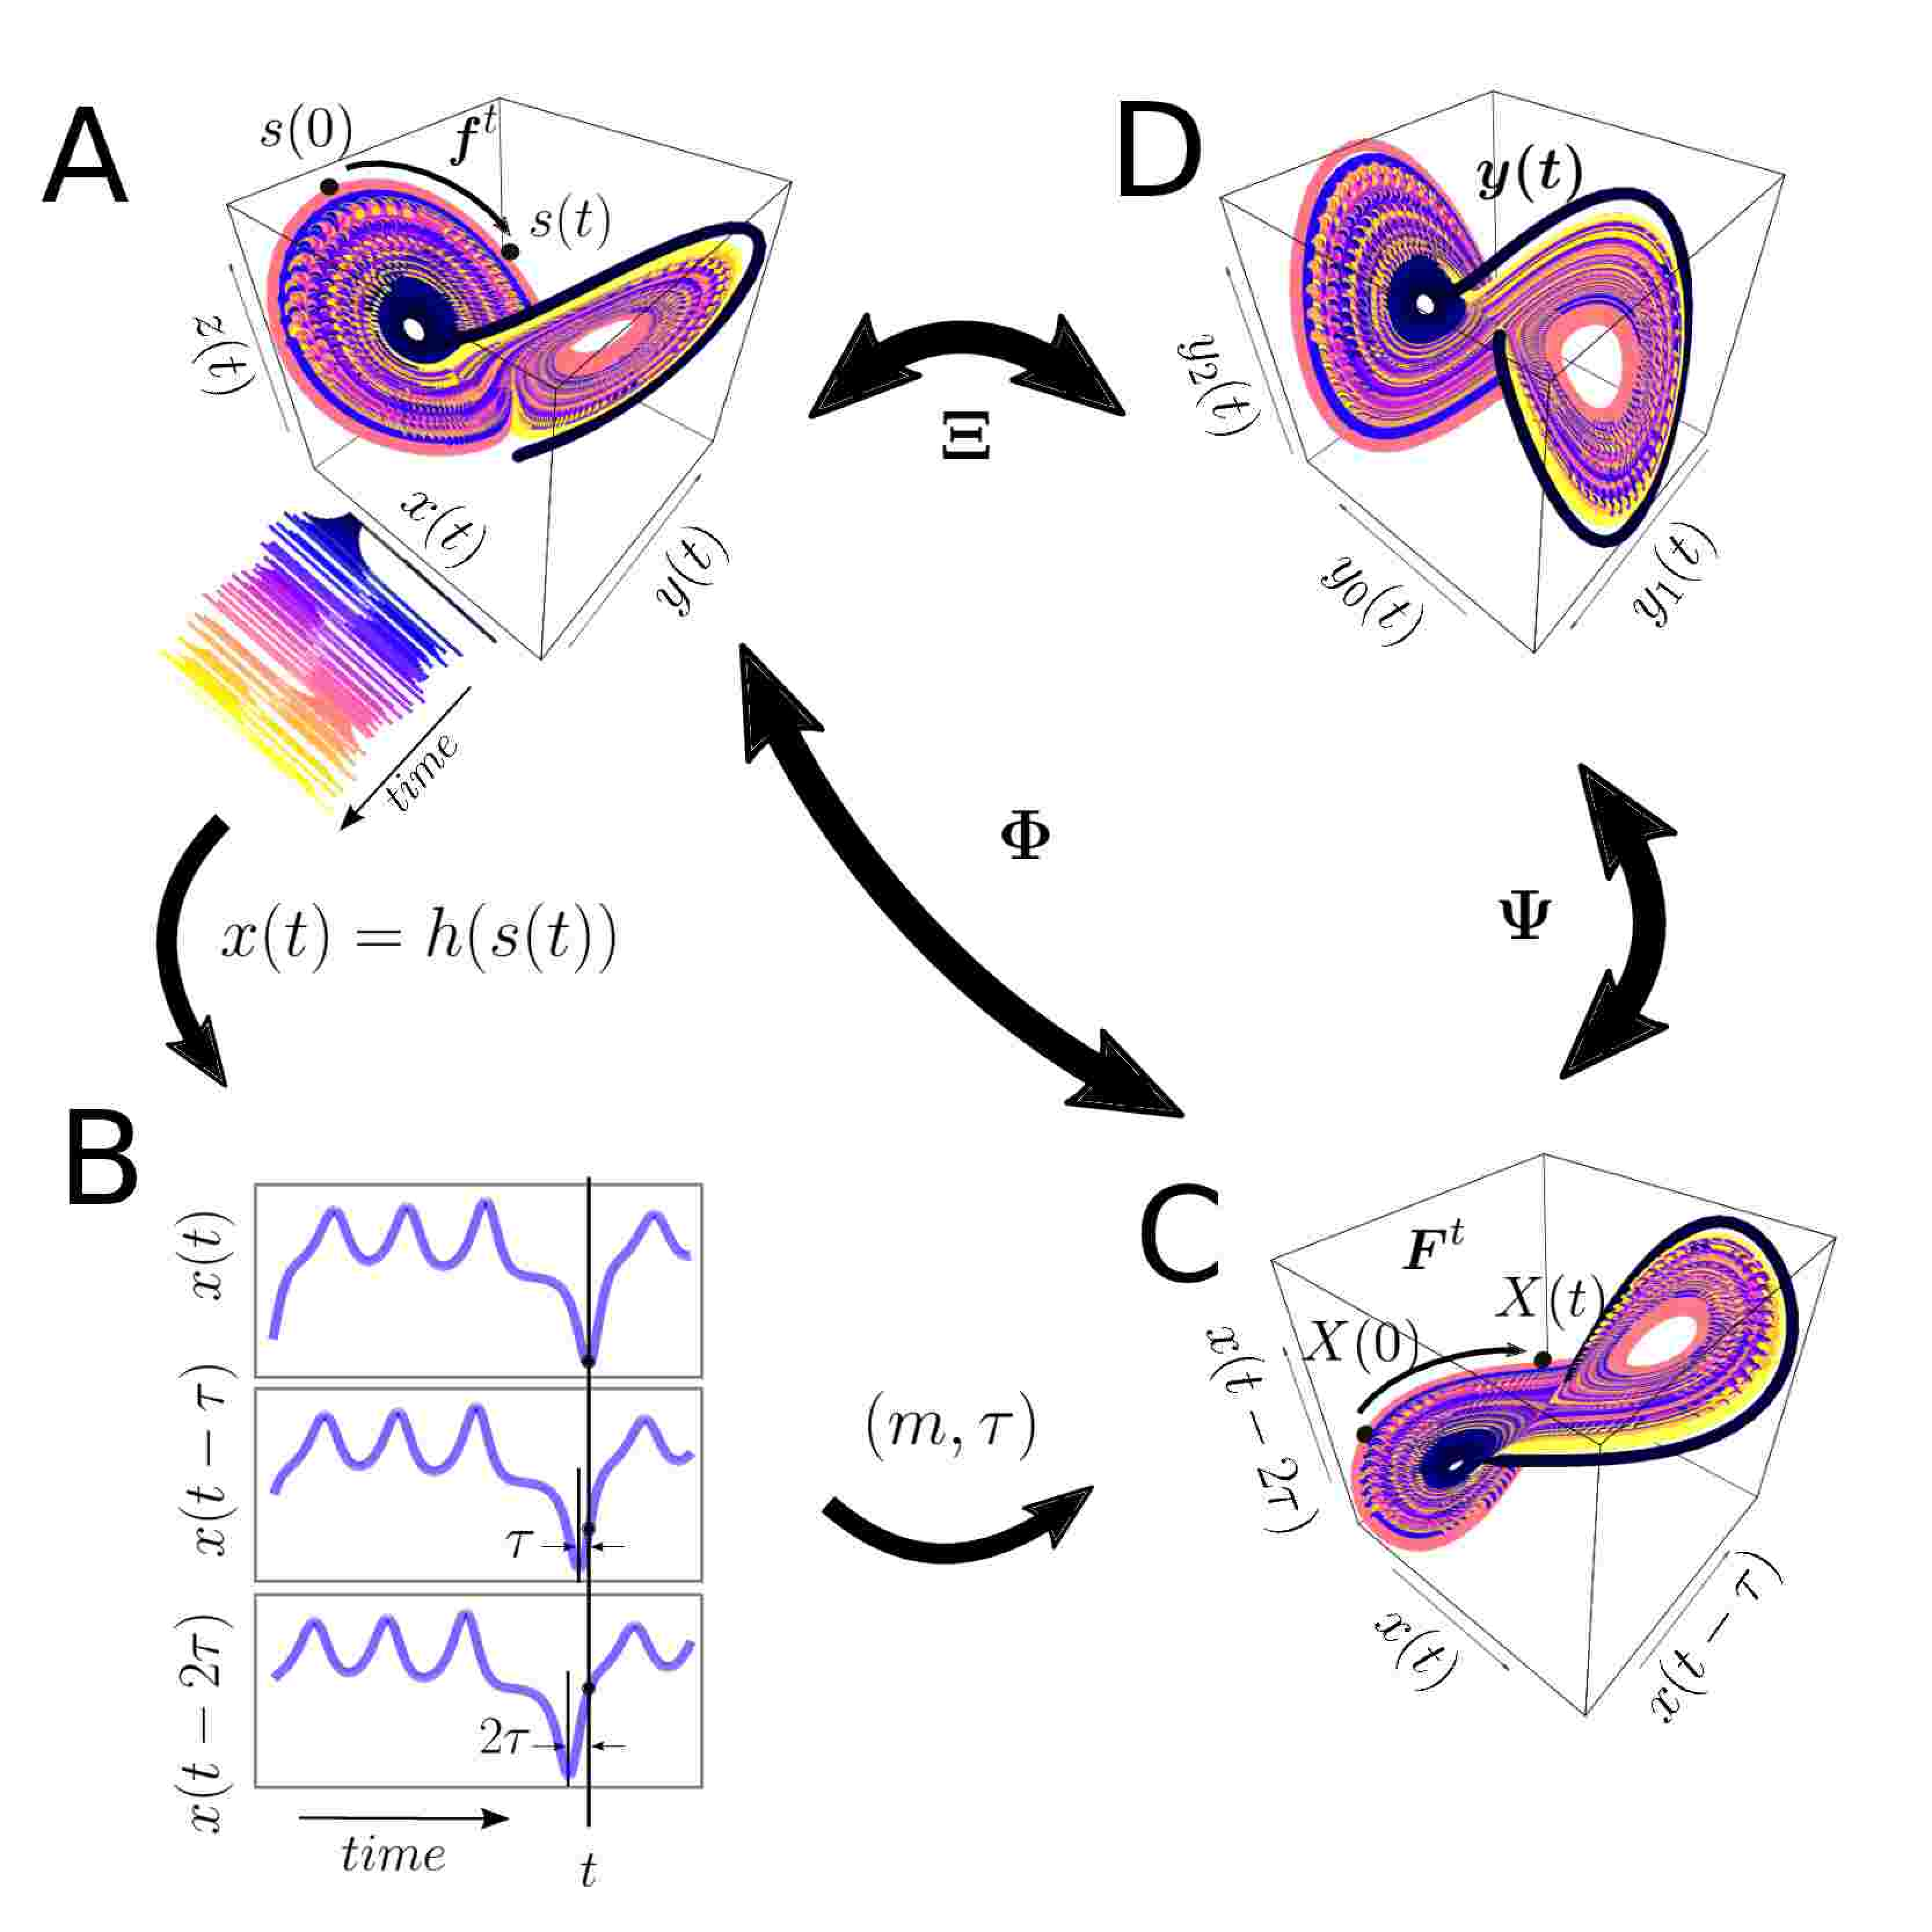
\includegraphics[width=1.0\textwidth]{fig-rss.pdf}
    \caption{
	{\bf State space reconstruction methodology.}
	State space reconstruction is based on $x(t)=h[s(t)]= h[f^t [s(0)]]$
	where $f^t$ is the true dynamical system, $s(t)$ indicates the state,
    	$s$, at time, $t$,  and $h[ ]$ the measurement function. 
    	The time-delay embedding represented as the $\Phi$, maps the original
    	$d-$dimensional state $s(t)$ into the $m-$dimensional uniform 
	time-delay embedding matrix $\boldsymbol{X}(t)$.
    	The transformation map $\Psi$ then maps $\boldsymbol{X}(t)$ into 
	a new state $y(t)$ of dimensions $n < m$.
    	(A) $M-$dimensional manifold representing the state space 
	(e.g. Lorenz system);
    	(B) Delayed copies of $1-$dimensional $x(t)$ from the Lorenz system;
   	(C) $m-$dimensional reconstructed state space with 
    	\texorpdfstring{$m$}{m} and    \texorpdfstring{$\tau$}{T}, and 
    	(D) $y(t)$ is the $n-$dimensional reconstructed state space.
	The total reconstruction map is represented as $\Xi = \Psi \circ \Phi $
	where $\Phi$ is the delay reconstruction map and 
	$\Psi$ is the coordinate transformation map.
	This figure is adapted from 
   	\cite{Quintana-Duque2012, casdagli1991, uzal2011}.
	Code and data to reproduce the figure is available in \cite{srep2020}.
    }
    \label{fig:ssr}
\end{figure}
%%---------------------------------(FIGURE)-------------------------------------



\subsection*{Uniform Time-Delay Embedding (UTDE)}\label{sec:utimedelayembedding}
Frank et al. and Sama et al. refer to the state space reconstruction
as "time-delay embeddings" or "delay coordinates" \cite{frank2010, sama2013}. 
However, we consider the term "uniform time-delay embedding"
as more descriptive and appropriate terminology for our work.
Hence, the uniform time-delay embedding is represented as a matrix of uniform delayed 
copies of the time series $\{ \boldsymbol{x}_n \}_{n=1}^N$ where $N$ is 
the sample length of $\{ \boldsymbol{x}_n \}$ and $n$ is index for the 
samples of $\{ \boldsymbol{x}_n \}$.
$\{ \boldsymbol{x}_n \}_{n=1}^N$ has a sample rate of $T$.
The delayed copies of $\{ \boldsymbol{x}_n \}$ are uniformly separated by $\tau$
and represented as $\{\boldsymbol{ \tilde{x} }_{n- i\tau} \}$
where $i$ goes from $0,1, \dots, (m-1)$.
Generally speaking, $\{\boldsymbol{ \tilde{x} }_{n- i\tau} \}$ contains
information of unobserved state variables and encapsulates the information of
the delayed copies of the available time series in the uniform time-delay 
embedding matrix $\boldsymbol{X}^{m}_{\tau}$, 
$\boldsymbol{X}^{m}_{\tau} \in \mathbb{R}^m$, defined as
%%********************************[EQUATION]************************************
\begin{equation}\label{eq:tde}
\boldsymbol{X}^{m}_{\tau}  =
\begin{pmatrix}
\boldsymbol{ \tilde{x} }_n \\
\boldsymbol{ \tilde{x} }_{n-\tau} \\
\boldsymbol{ \tilde{x} }_{n-2\tau} \\
\vdots \\
\boldsymbol{ \tilde{x} }_{n- (m-1) \tau} \\
\end{pmatrix}^\intercal, 
\end{equation}
%%********************************[EQUATION]************************************
where $m$ is the embedding dimension, $\tau$ is the embedding delay and
$ ^\intercal$ denotes the transpose.
$m$ and $\tau$ are known as embedding parameters.
The matrix dimension of $ \boldsymbol{X}_{\tau}^{m} $ is defined by
$N-(m-1)\tau$ rows and $m$ columns and 
$N-(m-1)\tau$ defines the length of each delayed copy 
of $\{ \boldsymbol{ \tilde{x} }_n \}$ in $\boldsymbol{X}^{m}_{\tau}$.
%For further details and explicit examples of uniform time-delay 
%embedding methodology, we refer the reader to the \nameref{S1_AppendixA}.




\subsection*{Estimation of Embedding Parameters}
The estimation of the embedding parameters ($m$ and $\tau$) 
is a fundamental step for the state space reconstruction with the use
of uniform time-delay embedding method.
With this in mind, we review two of the most common algorithms,
which will be used in our work, to compute the embedding
parameters: the false nearest neighbour (FNN) and the average mutual information (AMI).

%%%%%%%%%%%%%%%%%%%%%%%%%%%%%%%%%%%%%%%%%%%%%%%%%%%%%%%%%%%%%%%%%%%%%%%%%%%%%%%%
%*******************************************************************************
\subsubsection*{False Nearest Neighbours}
To select the minimum embedding dimension $m_0$, Kennel et al. \cite{kennel1992}
used the method of false neighbours which can be understood as follows:
on the one hand, when the embedding dimension is too small to unfold the 
attractor "not all points that lie close each other will be neighbours and 
some points appear as neighbours because of the attractor has been projected 
down into an smaller space", on the other hand, when increasing the embedding 
dimension "points that are near to each other in the sufficient
embedding dimension should remain close as the dimension increase from $m$ 
to $m+1$ \cite{krakovska2015}".
From a mathematical point of view, the state space reconstruction theorem is 
done when the attractor is unfolded with either the minimum embedding 
dimension, $m_0$, or any other embedding dimension value where 
$m \ge m_0$ \cite{kennel1992}. On the contrary, any large value of $m_0$ 
leads to excessive computations \cite{bradley2015}. With this in mind, 
Cao \cite{Cao1997} proposed an algorithm based on the false neighbour method 
where only the time-series and one delay embedding value are necessary 
to select the minimum embedding dimension. Cao's algorithm is based 
on $E(m)$  which is the mean value of all $a(i,m)$, both defined as follows
%%********************************[EQUATION]************************************
\begin{equation}\label{eq:e}
  \begin{aligned}
	E(m) &= \frac{1}{N-m\tau} \sum_{i=1}^{N-m\tau} a(i,m) \\
	 &=
       \frac{1}{N-m\tau} \sum_{i=1}^{N-m\tau}
       \frac{ || \boldsymbol{X}_i(m+1) - \boldsymbol{X}_{n(i,m)}(m+1) || }
            { || \boldsymbol{X}_i(m) - \boldsymbol{X}_{n(i,m)}(m) ||  }
  \end{aligned}
\end{equation}
%%********************************[EQUATION]************************************
where $\boldsymbol{X}_i(m)$ and $\boldsymbol{X}_{n(i,m)}(m)$ are the time-delay
embeddings with $i=1,2,\dots,N-(m-1)\tau$ and $ n(i,m)= 1 \le n(i,m) \le N-m\tau$.
From Eq.~\ref{eq:e}, it can be seen that $E(m)$ is only dependent on $m$ 
and $\tau$ for which $E_1(m)$ is defined as
%%********************************[EQUATION]************************************
\begin{equation}\label{eq:e1}
E_1(m) = \frac{ E(m+1) } { E(m)}.
\end{equation}
%%********************************[EQUATION]************************************
$E_1(m)$ is therefore considered to investigate the variation from $m$ to $m+1$
in order to find the minimum embedding dimension $m_0$ (Eq.~\ref{eq:e1}).
As described in \cite{Cao1997}: "$E_1(m)$ stops changing when $m$ is greater
than some $m_0$, if the time series comes from a multidimensional state space
then $m_0 + 1$ is the minimum dimension".
Additionally, Cao proposed $E_2(m)$ to distinguish deterministic signals from
stochastic signals. $E_2(m)$ is defined as
%%********************************[EQUATION]************************************
\begin{equation}\label{eq:e2}
E_2(m) = \frac{ E^* (m+1) } { E^*(m)},
\end{equation}
%%********************************[EQUATION]************************************
where
%%********************************[EQUATION]************************************
\begin{equation}\label{eq:ee}
E^*(m) = \frac{1}{N-m\tau} \sum_{i=1}^{N-m\tau}
|  \boldsymbol{X}_i(m+1) - \boldsymbol{X}_{n(i,m)}(m+1) |.
\end{equation}
%%********************************[EQUATION]************************************
For instance, when the signal comes from random noise (values that are 
independent from each other), all $E_2(m)$ values are approximately equal 
to 1 (e.g. $E_2(m) \approx 1$). However, for deterministic data $E_2(m)$ is 
not constant for all $m$ (e.g. $E_2(m) \neq 1$).

As an example of the use of $E_1(m)$ and $E_2(m)$ values, we consider two time 
series: the solution for the $x$ variable of the Lorenz system 
(Fig~\ref{fig:caoami}A), and a Gaussian noise time series with zero mean 
and a variance of one (Fig~\ref{fig:caoami}B).
We then compute $E_1(m)$ and $E_2(m)$ values for each time series.
The $E_1(m)$ values for the chaotic time series appear to be constant
after the dimension is equal to six.
The determination of six is given that any value of $m$ can be used as they 
are within the threshold of $1\pm0.05$ (Fig~\ref{fig:caoami}C).
$E_2(m)$ values, for chaotic time series, are different to one 
(Fig~\ref{fig:caoami}E), for which, it can be concluded that for the 
chaotic time series the minimum embedding dimension the time series 
comes from a deterministic signal. With regard to the noise time series,  
$E_1(m)$ values appeared to be constant when $m$ is close to thirteen, 
which is defined by the threshold of $1\pm0.05$ (Fig~\ref{fig:caoami}D).
$E_1(m)$ values then indicate the minimum embedding dimension of the 
noisy time series is thirteen, however all of the $E_2(m)$ values are 
approximately equal to one (Figure~\ref{fig:caoami}F) for which it can be 
concluded that noise time series is a stochastic signal.
It is important to note that for this work not only $E_1(m)$ and $E_2(m)$ are 
computed but also a variation of $\tau$ from 1 to 20 is presented. 
The purpose of such variation for $\tau$ is to show its independence with
regard to $E_1(m)$ and $E_2(m)$ values as $\tau$ is increasing 
(Fig~\ref{fig:caoami}C,D,E and F). 
However, one negative of the Cao's algorithm \cite{Cao1997} is the definition of 
a new threshold where $m$ values appear to be constant in $E_1 (m)$.
In the case of the given examples and reported results, we defined such 
threshold as 0.05. Further investigation is required for the selection of the 
threshold in the $E_1(m)$, as the selection of the threshold in this work is 
base on no particular method but visual inspection.

%%%%%%%%%%%%%%%%%%%%%%%%%%%%%%%%%%%%%%%%%%%%%%%%%%%%%%%%%%%%%%%%%%%%%%%%%%%%%%%%
%*******************************************************************************
\subsubsection*{Average Mutual Information}
When selecting the delay dimension parameter, $\tau$, one can consider the 
following two cases:
(i) when $\tau$ is too small, the elements of time-delay embedding will be along
the bisectrix of the phase space and the reconstruction is generally not 
satisfactory, 
(ii) on the contraty, when $\tau$ is too large the elements of the uniform 
time-delay embedding will become spread and uncorrelated which makes 
recovering the underlying attractor more difficult if not 
impossible \cite{casdagli1991, emrani2014a, garcia2005e71}.
With regard to the algorithms to compute $\tau$, 
Emrani et al. \cite{emrani2014a}, for instance, used the autocorrelation 
function in which the first zero crossing is considered as the minimum delay 
embedding parameter. However, the autocorrelation function is a linear 
statistic over which the Average Mutual Information (AMI) algorithm is 
preferred because the AMI takes into account the nonlinear dynamical 
correlations \cite{afraser1986,krakovska2015}. With this in mind, the AMI 
algorithm is described below to estimate the minimum delay embedding 
parameter, \texorpdfstring{$\tau_0$}{T}.

To compute the AMI, an histogram of $x(n)$ using $n$ bins is calculated
and then a probability distribution of data is computed \cite{kantz2003}.
AMI is therefore denoted by $I(\tau)$ which is the average mutual 
information between the original time series, $x(n)$, and the delayed 
time series, $x(n-\tau)$, delayed by $\tau$ \cite{kabiraj2012}. 
AMI is defined by
%%********************************[EQUATION]************************************
\begin{equation}\label{eq:ami}
I(\tau) = \sum_{i,j}^N p_{ij} log_2 \frac{ p_{ij} }{ p_i p_j }.
\end{equation}
%%********************************[EQUATION]************************************
Probabilities are defined as follows:
$p_i$ is the probability that $x(n)$ has a value inside the $i$-th bin of 
the histogram, $p_j$ is the probability that $x(n+\tau)$ has a value inside 
the $j$-th bin of the histogram and $p_{ij}(\tau)$ the probability 
that $x(n)$ is in bin $i$ and $x(n+\tau)$ is in bin $j$. The AMI is measured 
in bits (base 2, also called shannons) \cite{kantz2003, nonlinearTseries2016}.
For small $\tau$, AMI will be large and it will then decrease more or 
less rapidly. As $\tau$ increase and goes to a large limit, 
$x(n)$ and $x(n+\tau)$ have nothing to do with each other and $p_(ij)$ is 
factorised as $p_ip_j$ for which AMI is close to zero. Then, in order 
to obtain $\tau_0$, "it has to be found the first minimum of $I(\tau)$ 
where $x(n+\tau)$ adds maximal information to the knowledge from $x(n)$, or,
where the redundancy is the least" \cite{kantz2003}.

For example, we compute the AMI for two time series:
A) the $x$ solution of the Lorenz system, and
B) a noise time series using a normal distribution with mean zero and 
standard deviation equal to one. From Fig~\ref{fig:caoami}(G, H), it can then be 
concluded that the amount of knowledge for any noise time series is zero 
for which the first minimum embedding parameter is $\tau_0=1$. 
On the contrary, the first minimum of the AMI for the chaotic time series 
is $\tau_0=17$ which is the value that maximize the independence 
between $x(n)$ and $x(n+\tau)$ in the reconstructed state space 
\cite{bradley2015}.
%%---------------------------------(FIGURE)-------------------------------------
Similarly as Cao's algorithm negatives, AMI's algorithm is not an
exception for negatives, which are worthwhile to mention for further 
investigations.
For instance, (i) is not clear why the choose of the first minimum of the AMI 
is the minimum delay embedding parameter \cite{kantz2003} and 
(ii) the probability distribution of the AMI function is computed
with the use of histograms which depends on a heuristic choice of number of bins
for which AMI depends on partitioning \cite{garcia2005e71}.

%%---------------------------------(FIGURE)-------------------------------------
\begin{figure}[ht]
\centering
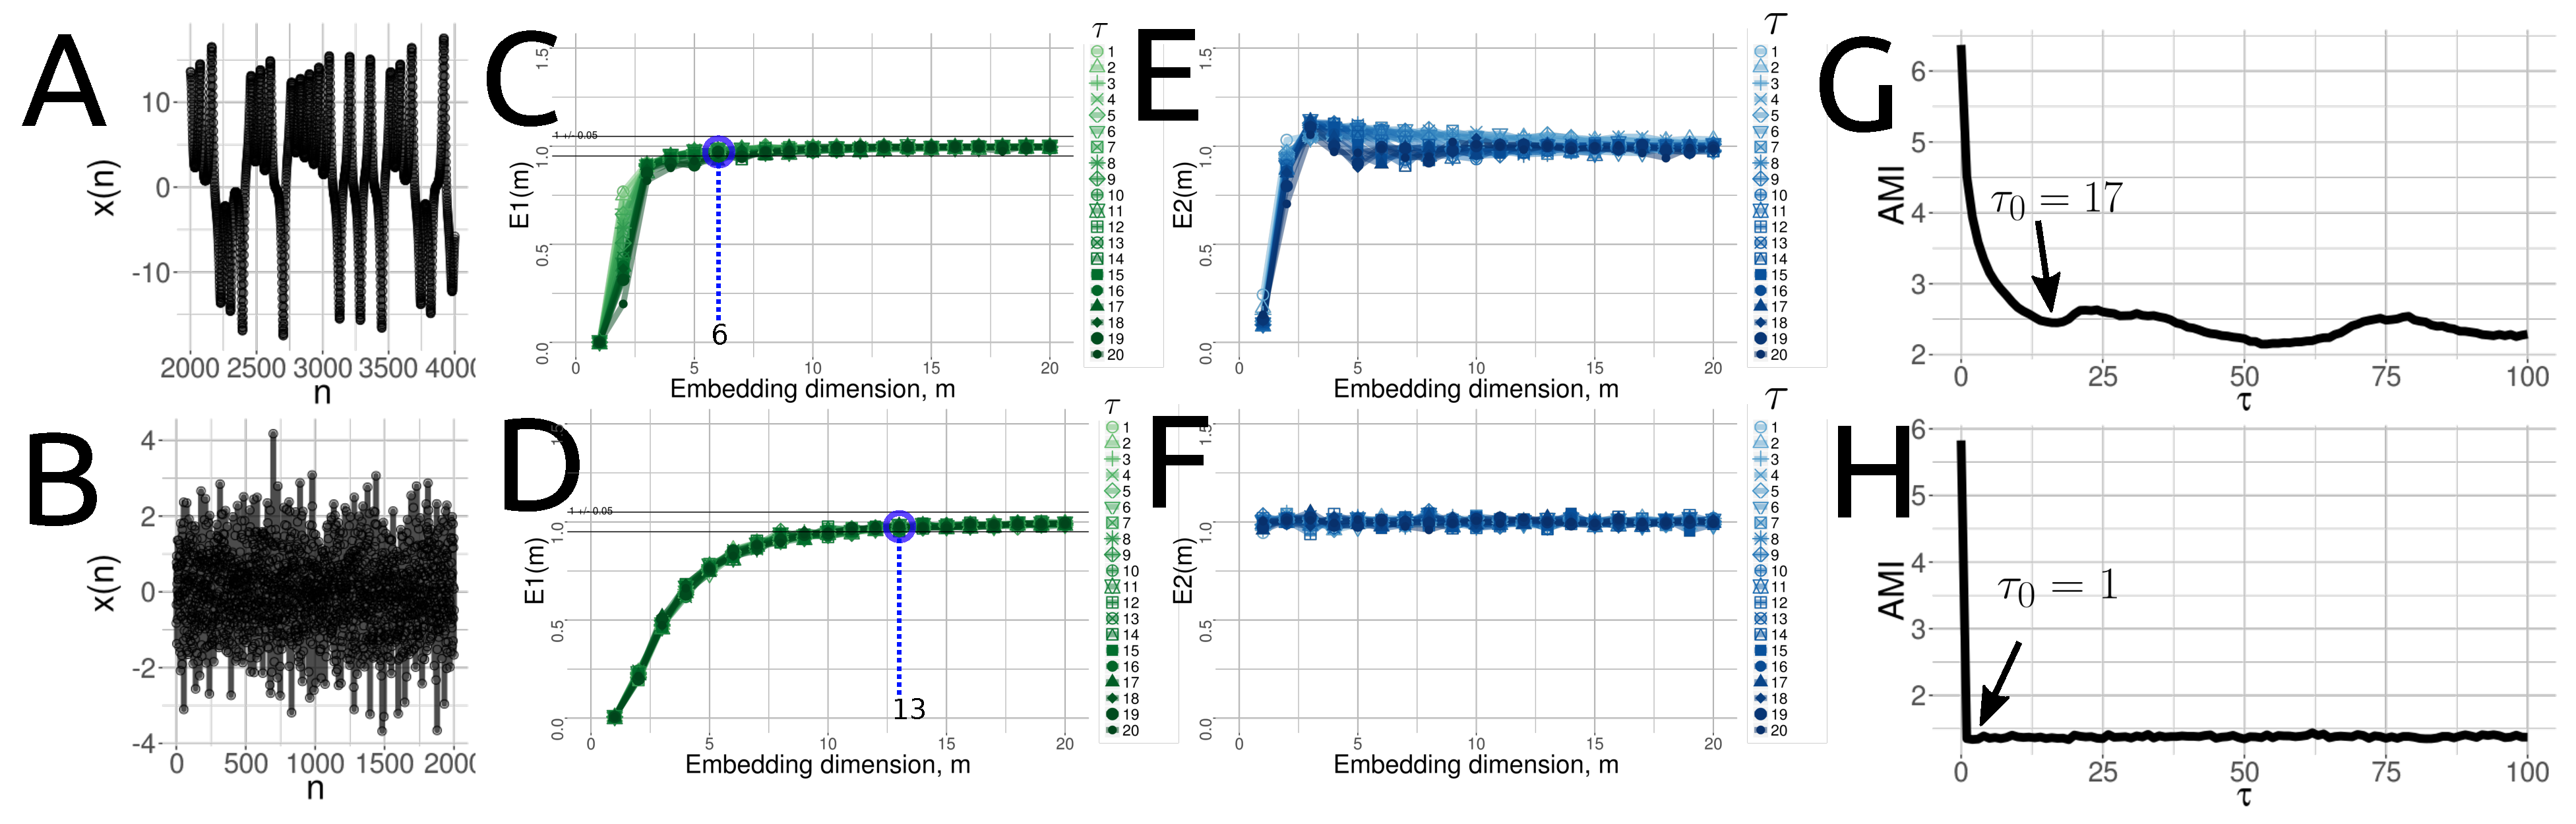
\includegraphics[width=1.0\textwidth]{fig-caoami.pdf}
    \caption{
	{\bf Minimum delay embedding values with AMI's method and minimum dimension embedding values with Cao's method.} 
	(A) chaotic and (B) random time series.
	(C, D) $E_1 (m)$ values and (E, F) $E_2(m)$ values 
	with variations of $\tau$ values from one to twenty
	for chaotic and random time series.
	(G, H) AMI values where its first minimum value in the curve
	is the minimum time delay embedding ($\tau_0$).
	Code and data to reproduce the figure is available in \cite{srep2020}.
        }
    \label{fig:caoami}
\end{figure}
%%---------------------------------(FIGURE)-------------------------------------


%*******************************************************************************
\section*{Recurrence Quantification}\label{sec:recurrence-quantification}
\subsection*{Recurrence Plots}
Originally, Henri Poincar\'e in 1890 introduced the concept of recurrences 
in conservative systems, however such discovery was not put into practice 
until the development of faster computers \cite{marwan2007},
for which Eckmann et al. \cite{eckmann1987} in 1987 introduced a method
where recurrences in the dynamics of a system can be visualised using 
Recurrence Plots. The intention of Eckmann et al. \cite{eckmann1987} was to 
propose a tool, called Recurrence Plot (RP), that provides insights into 
high-dimensional dynamical systems where trajectories are very difficult to 
visualise. Therefore, "RP helps us to investigate the 
$m-$dimensional phase space trajectories through a two-dimensional 
representation of its recurrences" \cite{marwan2015}.
Similarly, Marwan et al. \cite{marwan2015} pointed out that additionally 
to the methodologies of the state space reconstruction and other dynamic 
invariants such as Lyapunov exponent, Kolmogorov-Sinai entropy, 
the recurrences of the trajectories in the phase space can provide 
important clues to characterise natural process that present, for
instance, periodicities (as Milankovitch cycles) or irregular cycles 
(as El Ni\~no Southern Oscillation). 
Such recurrences can not only be presented visually using Recurrence Plots (RP) 
but also be quantified with Recurrence Quantification metrics, which leads 
to applications of these in various areas such as economy, physiology, 
neuroscience, earth science, astrophysics and engineering \cite{marwan2007}.

For the creation of a recurrence plot based on time series 
$\{ \boldsymbol{x}_n \}$, it is first computed the state space 
reconstruction with uniform time-delay embedding 
$X(i)=\{ \boldsymbol{ \tilde{x} }_n, \dots,  
\boldsymbol{ \tilde{x} }_{n -(m-1)\tau} \}$
where $i=1,\dots,N$, $N$ is the number of considered states of $X(i)$ 
and $X(i) \in \mathbb{R}^m$ \cite{eckmann1987}.
The recurrence plot is therefore a two-dimensional $N \times N$ square 
matrix, $\mathbf{R}$, where a black dot is placed at $(i,j)$ 
whenever $X(i)$ is sufficiently close to $X(j)$: 
%%********************************[EQUATION]************************************
\begin{equation}
\mathbf{R}^{m}_{i,j} (\epsilon) = \Theta ( \epsilon_i - || X(i) - X(j) ||
\end{equation}
%%********************************[EQUATION]************************************
where $\quad i,j=1,\dots,N$, $\epsilon$ is a threshold distance, 
$|| \cdotp ||$ a norm, and $\Theta(\cdotp)$ is the Heaviside 
function (i.e. $\Theta(x)=0$, if $x<0$, and $\Theta(x)=1$ otherwise) 
(Fig~\ref{fig:rps}(A,B)) \cite{eckmann1987, marwan2007,marwan2015}.
RP is also characterised with a line of identity (LOI) which is a  
diagonal line due to $ R_{i,j}=1 (i,j=1,\dots,N)$. 


%*******************************************************************************
%*******************************************************************************
%*******************************************************************************
\subsection*{Structures of Recurrence Plots}
Pattern formations in the RPs can be designated either 
as topology for large-scale patterns or texture for small-scale patterns.
In the case of topology, the following pattern formations are commonly presented:
(i) homogeneous where uniform recurrence points are spread in the RP e.g., 
uniformly distributed noise (Fig~\ref{fig:rps}C), 
(ii) periodic and quasi-periodic systems where diagonal lines and 
checkerboard structures represent oscillating systems, e.g., sinusoidal 
signals (Fig~\ref{fig:rps}D), 
(iii) drift where paling or darkening recurrence points away from 
the LOI is caused by drifting systems, 
e.g., logistic map (Fig~\ref{fig:rps}E), and
(iv) disrupted where recurrence points are presented white areas or 
bands that indicate abrupt changes in the dynamics, e.g. Brownian motion 
(Fig~\ref{fig:rps}F) \cite{eckmann1987, marwan2015}.
Texture patterns in RPs can be categorised as:
(i) single or isolated recurrence points that represent rare occurring states, 
and do not persist for any time or fluctuate heavily,
(ii) dots forming diagonal lines where the length of the small-scale parallel 
lines in the diagonal are related to the ratio of determinism or predictability 
in the dynamics of the system, and
(iii) dots forming vertical and horizontal lines where the length of the 
lines represent a time length where a state does not change or change very 
slowly and these patterns formation represent discontinuities in the signal, 
and (iv) dots clustering to inscribe rectangular regions which are related 
to laminar states or singularities \cite{marwan2015}.

Although, each of the previous pattern descriptions of the structures in the 
RP offer an idea of the characteristics of dynamical systems, 
these might be misinterpreted and conclusions might tend to be subjective 
as these require the interpretation of a particular researcher(s).
Because of that, recurrence quantification analyis (RQA) offer objective 
methodologies to quantify such visual characteristics of previous 
recurrent pattern structures in the RP \cite{zbilut1992}.

%---------------------------------(FIGURE)-------------------------------------
\begin{figure}[ht]
\centering
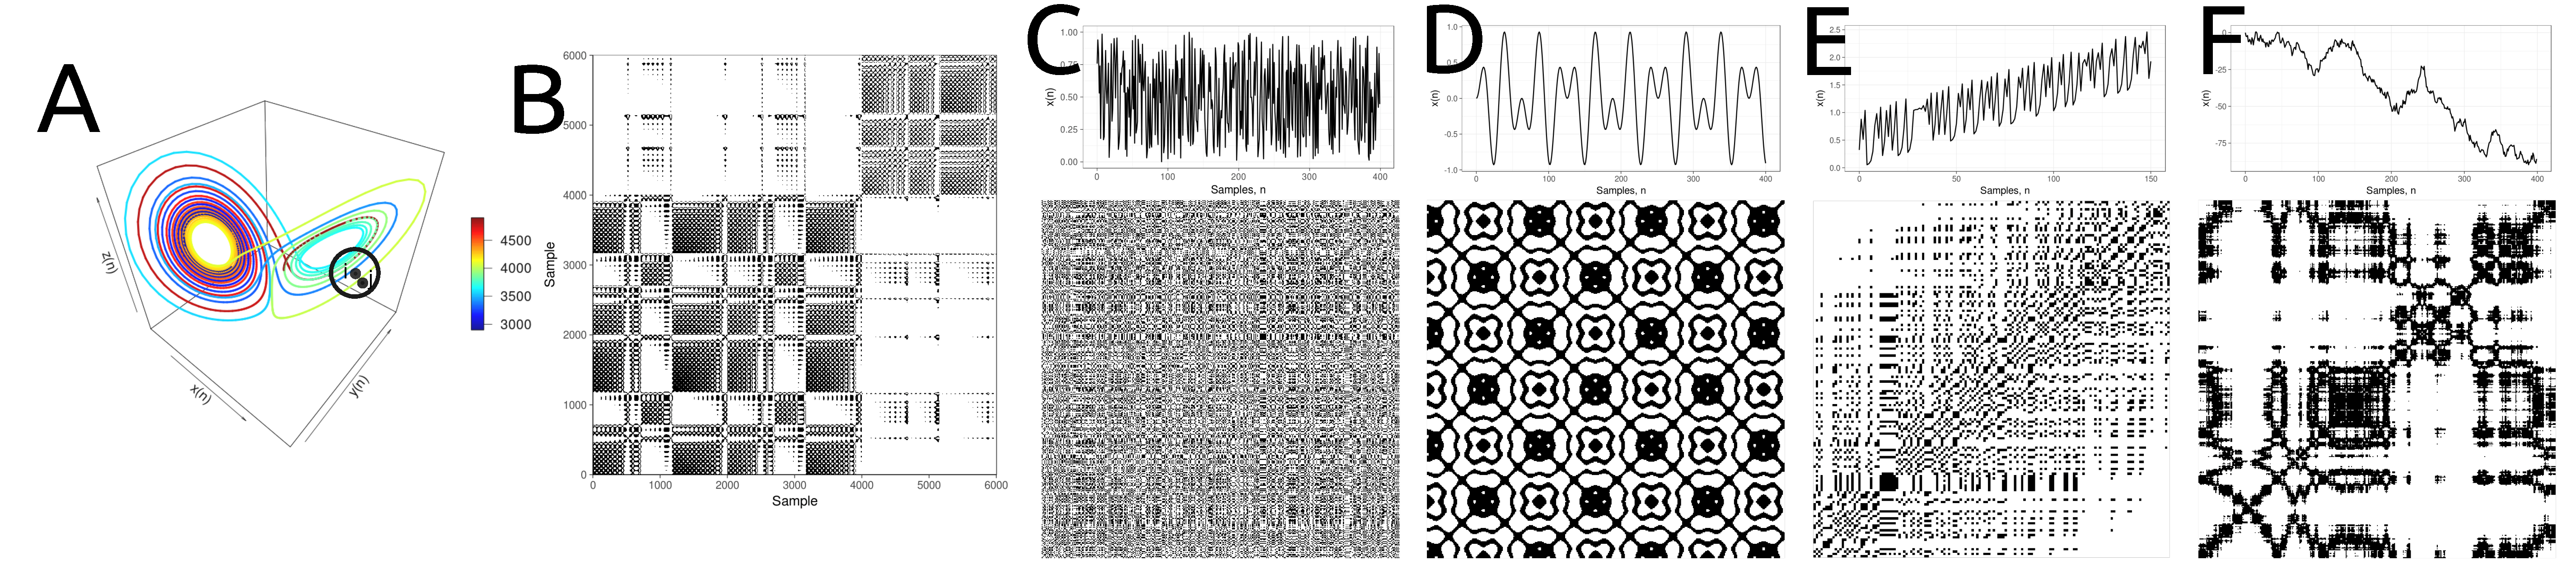
\includegraphics[width=1.0\textwidth]{fig-rps.pdf}
    \caption{
	{\bf Recurrence Plots and its patterns.} 
	(A) State space of the Lorenz system with controlling parameters 
	($\rho=28, \sigma=10, \beta=8/3$) where the point, $j$, in trajectory $X()$ which falls into the neighborhood 
	(black circle) of a given point at $i$ is a recurrent point and is 
	represented as a black dot in the recurrence plot at location 
	$(i, j)$ or white otherwise.
	(B) Recurrence plot using the 
	three components of the Lorenz system and the RP with no embeddings 
	and threshold $\epsilon=5$.
	Time-series with its respective recurrence plot for:
	(C) uniformly distributed noise,
	(D) super-positionet harmonic oscillation 
	($sin( \frac{1}{5}*t) * sin( \frac{5}{100}*t) $),
	(E) drift logistic map ($x_{i+1} = 4 x_i (1- x_i) $) corrupted 
	with a linearly increase term ($0.01*i$), and
	(F) disrupted brownian motion  ($x_{i+1} = x_i + 2*rnorm(1) $).
	This figure is adapted from \cite{marwan2015}.
	Code and data to reproduce the figure is available in \cite{srep2020}.
	}
    \label{fig:rps}
\end{figure}
%%---------------------------------(FIGURE)-------------------------------------



%*******************************************************************************
\subsection*{Recurrence Quantifications Analysis (RQA)}
Originally, Zbilut et al. \cite{zbilut1992} proposed metrics to investigate 
the density of recurrence points in RPs, then histograms of lengths for 
diagonal lines in RPs were studied by \cite{trulla1996} which were the 
introduction to the term recurrence quantification analysis (RQA) 
\cite{marwan2008}. RQA has been applied in many fields such as life science, 
engineering, physics, and others \cite{marwan2008}. Particularly in human 
movement to investigate noise and complexity of postural control 
\cite{rhea2011}, postural control \cite{apthorp2014} or interpersonal 
coordination \cite{duran2017}. The success of RQA is not only due to its 
simple algorithmic implementation but also to its capacity to detect tiny 
modulations in frequency or phase which are not detectable using standard 
methods e.g. spectral or wavelet analysis \cite{marwan2011}, and that 
RQA's metrics are quantitatively and qualitatively independe]nt of embedding 
dimension which is verified experimentally by \cite{iwanski1998}.
RQA metrics comprehend percentage of recurrence, percentage of determinism, 
ratio, Shannon entropy of the frequency distributions of the line lengths,
maximal line length and divergence, trend and laminariy 
\cite{marwan2007, marwan2015}. For this work, we considered only four 
RQA metrics, due to its consistency with our preliminary experiments, 
which are described below. Such metrics are computed the nonlinearTseries 
R package \cite{nonlinearTseries2016}.

\subsubsection*{REC values}
The percentage of recurrence (REC) is defined as
%%********************************[EQUATION]************************************
\begin{equation}
REC(\epsilon,N) = 
		\frac{1}{N^2 - N} \sum^{N}_{i \neq j = 1} 
		\mathbf{R}^{m}_{i,j}(\epsilon),
\end{equation}
%%********************************[EQUATION]************************************
which enumerates the black dots in the RP excluding the line of identity.
REC is a measure of the relative density of recurrence points in the sparse 
matrix \cite{marwan2015}.
%REC is computed as follow with the nonlinearTseries package 
% \cite{nonlinearTseries} 
%  hist = getHistograms(neighs, ntakens, lmin, vmin)
%  # calculate the number of recurrence points from the recurrence rate. The
%  # recurrence rate counts the number of points at every distance in a concrete
%  # side of the main diagonal.
%  # Thus, sum all points for all distances, multiply by 2 (count both sides) and
%  # add the maindiagonal
%  numberRecurrencePoints = sum(hist$recurrenceHist) + ntakens
%  # calculate the recurrence rate dividing the number of recurrent points at a
%  # given distance by all points that could be at that distance
%  recurrence_rate_vector = 
%  hist$recurrenceHist[1:(ntakens - 1)] / ((ntakens - 1):1)
%  # percentage of recurrent points
%  REC = (numberRecurrencePoints) / ntakens ^ 2

\subsubsection*{DET values} 
The percent determinism (DET) is defined as the fraction of recurrence points
that form diagonal lines and it is determined by
%%********************************[EQUATION]************************************
\begin{equation}
DET=
	\frac{\sum^{N}_{l=d_{min}} l H_D{l} }
	     {\sum^{N}_{i,j=1} \mathbf{R}_{i,j}(\epsilon) },
\end{equation}
%%********************************[EQUATION]************************************
where 
%%********************************[EQUATION]************************************
\begin{equation}
H_D(l) = 
	\sum^{N}_{i,j=1} 
	(1- \mathbf{R}_{i-1,j-1}(\epsilon) ) 
	(1- \mathbf{R}_{i+l,j+l}(\epsilon) ) 
	\prod^{l-1}_{k=0}  \mathbf{R}_{i+k,j+k}(\epsilon)
\end{equation}
%%********************************[EQUATION]************************************
is the histogram of the lengths of the diagonal structures in the RP.
DET can be interpreted as the predictability of the system for periodic signals 
which, in essence, have longer diagonal lines than the short diagonals lines
for chaotic signals or absent diagonal lines for stochastic signals 
\cite{marwan2007, marwan2015}. Similarly, DET is considered as a measurement for 
the organisation of points in RPs  \cite{iwanski1998}. 
%percent determinism (DET) is computed as follow with the nonlinearTseries 
%package \cite{nonlinearTseries}  
% calculateDiagonalParameters = function(ntakens, numberRecurrencePoints,
%                                       lmin = 2, lDiagonalHistogram,
%                                       recurrence_rate_vector, maxDistanceMD) {
%  #begin parameter computations
%  num = sum((lmin:ntakens) * lDiagonalHistogram[lmin:ntakens])
%  DET = num / numberRecurrencePoints


\subsubsection*{RATIO values}
RATIO is defined as the ratio between DET and REC and it is calculated from 
the frequency distributions of the lengths of the diagonal lines.
RATIO is useful to discover dynamic transitions \cite{marwan2015}.
%  diagP = calculateDiagonalParameters(
%    ntakens, numberRecurrencePoints, lmin, hist$diagonalHist,
%    recurrence_rate_vector, maxDistanceMD
%  )
% calculateDiagonalParameters = function(ntakens, numberRecurrencePoints,
%                                       lmin = 2, lDiagonalHistogram,
%                                       recurrence_rate_vector, maxDistanceMD) {
%  #begin parameter computations
%  num = sum((lmin:ntakens) * lDiagonalHistogram[lmin:ntakens])
%  DET = num / numberRecurrencePoints
% 
%
%    RATIO = diagP$DET / REC
%

\subsubsection*{ENT values}
ENT is the Shannon entropy of the frequency distribution of the diagonal 
line lengths and it is defined as
%%********************************[EQUATION]************************************
\begin{equation}
ENT= - \sum^{N}_{l=d_{min}} p(l) ln p(l) \quad with 
	\quad p(l)=\frac{ H_D(l) }{ \sum^{N}_{ l=d_{min} } H_D(l) }.
\end{equation}
%%********************************[EQUATION]************************************
ENT reflects the complexity of the deterministic structure in the system.
For instance, for uncorrelated noise or oscillations, 
the value of ENT is rather small and indicates low complexity of the system,
therefore "the higher the ENT is the more complex the dynamics are" 
\cite{marwan2007, marwan2015}.
%#'  \item \emph{ENTR}: Shannon entropy of the diagonal line lengths distribution
%
%calculateDiagonalParameters = function(ntakens, numberRecurrencePoints,
%                                       lmin = 2, lDiagonalHistogram,
%                                       recurrence_rate_vector, maxDistanceMD) {
%
%  pl = lDiagonalHistogram / sum(lDiagonalHistogram)
%  diff_0 = which(pl > 0)
%  ENTR = -sum(pl[diff_0] * log(pl[diff_0]))

 
\subsection*{Sensitivity and robustness of RPs and RQA.}
RP and RQA are a very young field in nonlinear dynamics and many questions 
are still open, for instance, different parameters for window length size 
of the time series, embedding parameters or recurrence threshold can 
generate different results in RQA's metrics \cite{marwan2011, eckmann1987}.

The selection of recurrence threshold, $\epsilon$, can depend on the system 
that is analysed. For instance, when studying dynamical invariants $\epsilon$ 
require to be very small, for trajectory reconstruction $\epsilon$ requires 
to have a large thresholds or when studying dynamical transition 
there is little importance about the selection of the threshold 
\cite{marwan2011}. Other criteria for the selection of $\epsilon$ is that 
the recurrence threshold  should be five times larger 
than the standard deviation of the observational noise
or the use of diagonal structures within the RP is suggested in order
to find the optimal recurrence threshold for (quasi-)periodic process 
\cite{marwan2011}.
Similarly, Iwanski et al. \cite{iwanski1998} highlighted the importance 
of choosing the right embedding parameters to perform RQA for which 
many experiments have to be performed using different parameters in order 
to have a better intuition of the nature of the time series and how 
this is represented by using RQA.

With that in mind, this work explores the sensitivity and robustness 
of the window size of time series, embedding parameters for RSS with UTDE 
and recurrence threshold for RP and RQA in order to gain a better insight 
into the underlying time series collected from inertial sensors in the 
context of human-humanoid imitation activities.
%Such changes of recurrence threshold values 
%can modify the patterns in RPs and therefore the values of RQA metrics.
%We therefore computed 3D surfaces to explore the sensibility and robustness of 
%embedding parameters and recurrence threshold in RQA  metrics. Following the 
%same methodology of computing 3D surfaces, we also considered variation of 
%window length size to present RQA metrics dependencies with embedding 
%parameters, recurrence thresholds and window length size.


%Choosing an appropriate recurrence threshold is crucial so as to get 
%meaningful representations in RP and RQA, however, 

%Iwansky et al. \cite{iwanski1998} stated that patterns in Recurrence Plots and 
%metrics for RQA are independent of embedding dimension parameters, 
%however, that is not the case when using 
%different recurrence thresholds. 


%Zbilut et al. \cite{zbilut1992} established RQA metrics with the aim of 
%determining embedding parameters, their method consisted on creating 3D 
%surfaces with RQA metrics with an increase of embedding parameters 
%($m$ and $\tau$), then Zbilut et al. \cite{zbilut1992} explored 
%fluctuations and gradual changes in the 3D surfaces that provide information 
%about the embeddings. Much recently, Marwan et al. \cite{marwan2015} 
%created 3D surfaces for visual selection of not only embedding parameters 
%but also recurrence thresholds. Following same methodologies, we explored 
%the stability and robustness of RQA metrics (REC, DET, RATIO and ENTR)
%using 3D surfaces by an unitary increase of the pair embedding 
%parameters ($0 \ge m \le 10$, $0 \ge \tau \le 10$) and a decimal increase 
%of 0.1 for recurrence thresholds ($ 0.2 \ge \epsilon \le 3 $) 
%(Fig.~\ref{fig:topo_rqas}).



%*******************************************************************************
%*******************************************************************************
%*******************************************************************************
\section*{Experiment} \label{sec:experiment}
We conducted an experiment in the context of human-humanoid imitation (HHI) 
activities where participants were asked to imitate simple horizontal and 
vertical arm movements performed by NAO, a humanoid robot \cite{gouaillier2009}.
Such simple movements were repeated ten times for the participant 
who copied NAO's arm movements in a face-to-face imitation activity.
Also, wearable inertial measurement unit (IMU) sensors were attached 
to the right hand of the participant and to the left hand of the robot 
(Figure~\ref{fig:hri} A,C). Data were then collected with four NeMEMSi 
IMU sensors with sampling rate of 50Hz provinding tri-axial data of the 
accelerometer, gyroscope and magnetometer sensors and quaternions 
\cite{Comotti2014}.
%%---------------------------------(FIGURE)-------------------------------------
\begin{figure}[ht]
  \centering
\includegraphics[width=1.0\textwidth]{fig-hri}
    \caption{
	{\bf Human-humanoid imitation activities.} 
    		Face-to-face human-humanoid imitation (HHI) activities for 
		(A) HHI of horizontal arm movement, 
		(B) Humanoid horizontal arm movement,
		(C) HHI of vertical arm movement, and 
		(D) Humanoid vertical arm movement.
        }
    \label{fig:hri}
\end{figure}
%%---------------------------------(FIGURE)------------------------------------

\subsection*{Participants}
Twenty-three participants,
from now on defined as $pN$ where $N$ is the number of participant, were 
invited to do the experiment. However, data for three participants were 
not used because the instructions for $p01$, who was the only left-handed,
were mistakenly given in a way that movements were performed different
from what had been planned, and for participants $p13$ and $p16$ 
data were corrupted because of problems with Bluetooth communications with sensors. 
With that in mind, data for twenty participants were analysed in this work.
Of the twenty participants, all of them are right-handed healthy participants 
of whom four are females and sixteen are males with a mean and standard 
deviation (SD) age of mean=19.8 (SD=1.39). 

\subsection*{Ethics}
All participants provided informed consent forms prior to participation 
in the experiment. Hence, the experiments were conducted in November 2016 and 
participants confirmed reading and understanding the participant information sheet of the 
experiments and were able to withdraw from the experiment at any time without giving
any reason. The design of the experiments adhered to the University of Birmingham
regulations, data were anonymised and videos were stored only on a 
personal computer in accordance with the Data Protection Act 1998. 
%Refer to Appendix D for further information about the ethics, 
%online participation information sheets and experiment check list.


\subsection*{Human-humanoid imitation activities}
For human-humanoid imitation (HHI) activities four neMEMSi sensors were used,
two of which were attached to the right hand of the participant and the 
other two to the left hand of the humanoid robot.
Then, each participant was asked to imitate repetitions of simple horizontal
and vertical arm movements performed by the humanoid robot in the following 
conditions:
(i) ten repetitions of horizontal arm movement at normal (HN) 
	and faster (HF) speed (Figure~\ref{fig:hri} A), and
(ii) ten repetitions of vertical arm movement at normal (VN) 
	and faster (VF) speed (Figure~\ref{fig:hri} C).
The normal and faster speed of arm movements is defined by the duration 
in number of samples of one repetition of NAO's arm movements. 
We select NAO's arm movements duration to distinguish between normal and 
faster arm movements as NAO's movements have less variation 
for such repetitive movements. 
The duration for one repetition of the horizontal 
arm movement at normal speed, HN, is 5 seconds considering 
that each repetition last around 250 samples.
For horizontal arm movement at faster speed, HF, each repetition were performed 
in 2 seconds which correspond to 90 samples of data.
The vertical arm movement at normal speed, VN, were performed  in 6 seconds 
which is around 300 samples of data. For vertical arm movement at 
faster speed, VF, each repetition lasts about 2.4 seconds which correspond 
to 120 samples of data.
To visualise the distinction between normal and faster speed for horizontal 
and vertical arm movements, Fig~\ref{fig:sts} shows smoothed time series 
for axes Z and Y of the gyroscope sensors with four window lengths: 
2-sec (100-samples), 5-sec (250-samples), 10-sec (500-samples) 
and 15-sec (750-samples).
%%---------------------------------(FIGURE)-------------------------------------
\begin{figure}[ht] 
\centering
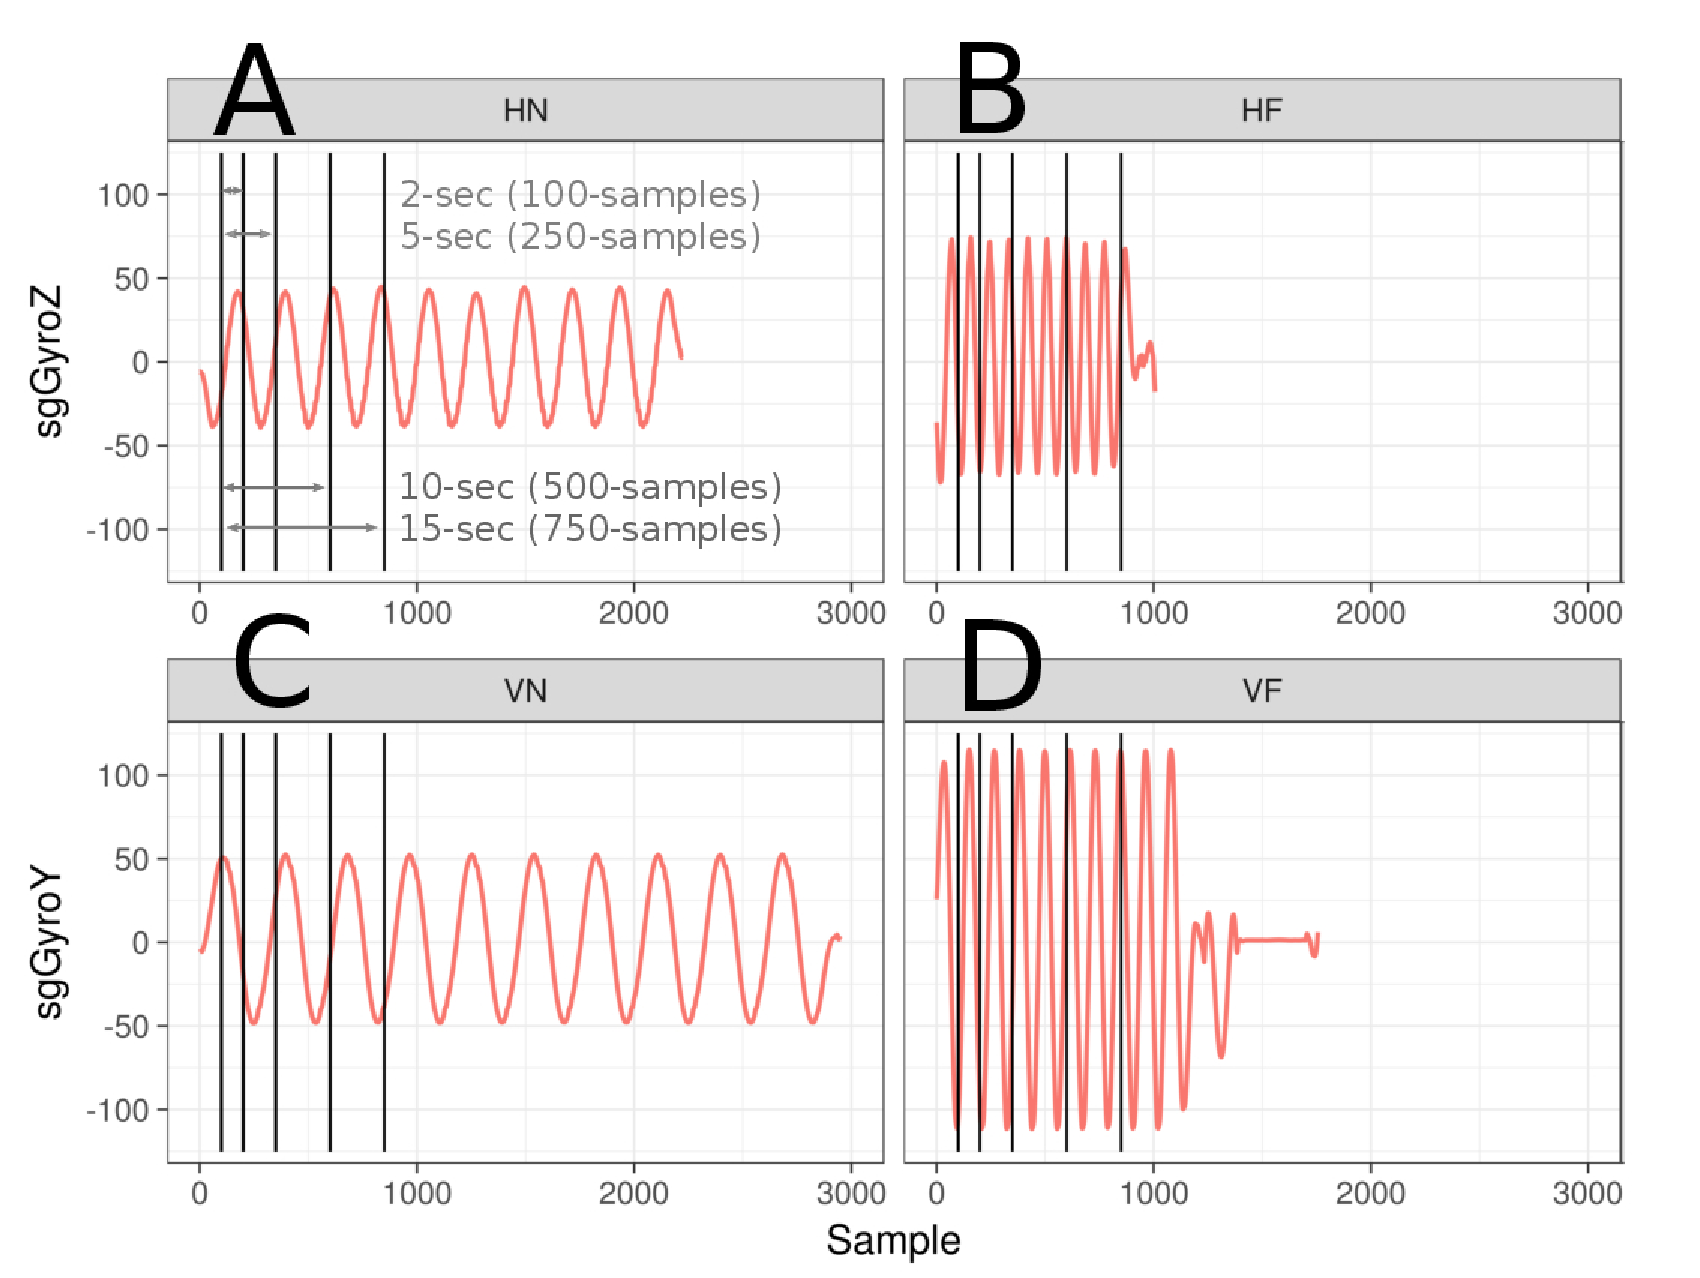
\includegraphics[width=1.0\textwidth]{fig-sts.pdf}
    \caption{
	{\bf Time series duration of horizontal and vertical arm movements.} 
    		Time series of smoothed data from gyroscope sensor 
		for different speed arm movements performed by NAO: 
		(A) Horizontal Normal arm movement (HN), 
		(B) Horizontal Faster arm movement (HF),
		(C) Vertical Normal arm movement (VN) and 
		(D) Vertical Faster arm movement (VF).
		Additionally, 
		(A) shows window sizes for 2-seconds (100 samples), 
		5-seconds (250 samples), 10-seconds (500 samples) 
		and 15-seconds (750 samples)
		which are also presented in (B), (C) and (D).
		Code and data to reproduce the figure is available in \cite{srep2020}.
        }
	\label{fig:sts}
\end{figure}
%%---------------------------------(FIGURE)------------------------------------

\subsection*{Data collection from inertial measurement units} 
\label{sec:experiment:subsec:imu}
To give insight to the research questions, 
we considered various conditions of time series collected for this work: 
\begin{itemize}
\item Three levels of smoothness for normalised data 
	(e.g., sg0zmuv, sg1zmuv and sg2zmuv) where sg 
	stands for Savitzky-Golay filter with two different filter lengths (29 and 159) 
	and the same polynomial degree of 5 using the function \texttt{sgolay(p,n,m)} \cite{Rsignal}
	and zmuv is zero mean unit variance.
\item four arm movement activities with two velocities: 
	horizontal normal (HN), horizontal faster (HF), 
	vertical normal (VN), and vertical faster (VF), and
\item four window lengths: 2-sec (100 samples), 5-sec (250 samples), 
	10-sec (500 samples) and 15-sec (750 samples).
\end{itemize}
%After the data collection, raw time series were windowed, normalised and smoothed. 
Due to space limitations and to have simple visualisation, 
we only present 10-sec (500 samples) window length time series for 
three participants (p01, p01 and p03) performing horizontal 
arm movements (axis GyroZ) and vertical arm movements (axis GyroY) (Figs \ref{fig:ts}).
%%---------------------------------(FIGURE)-------------------------------------
\begin{figure}[ht]
\centering
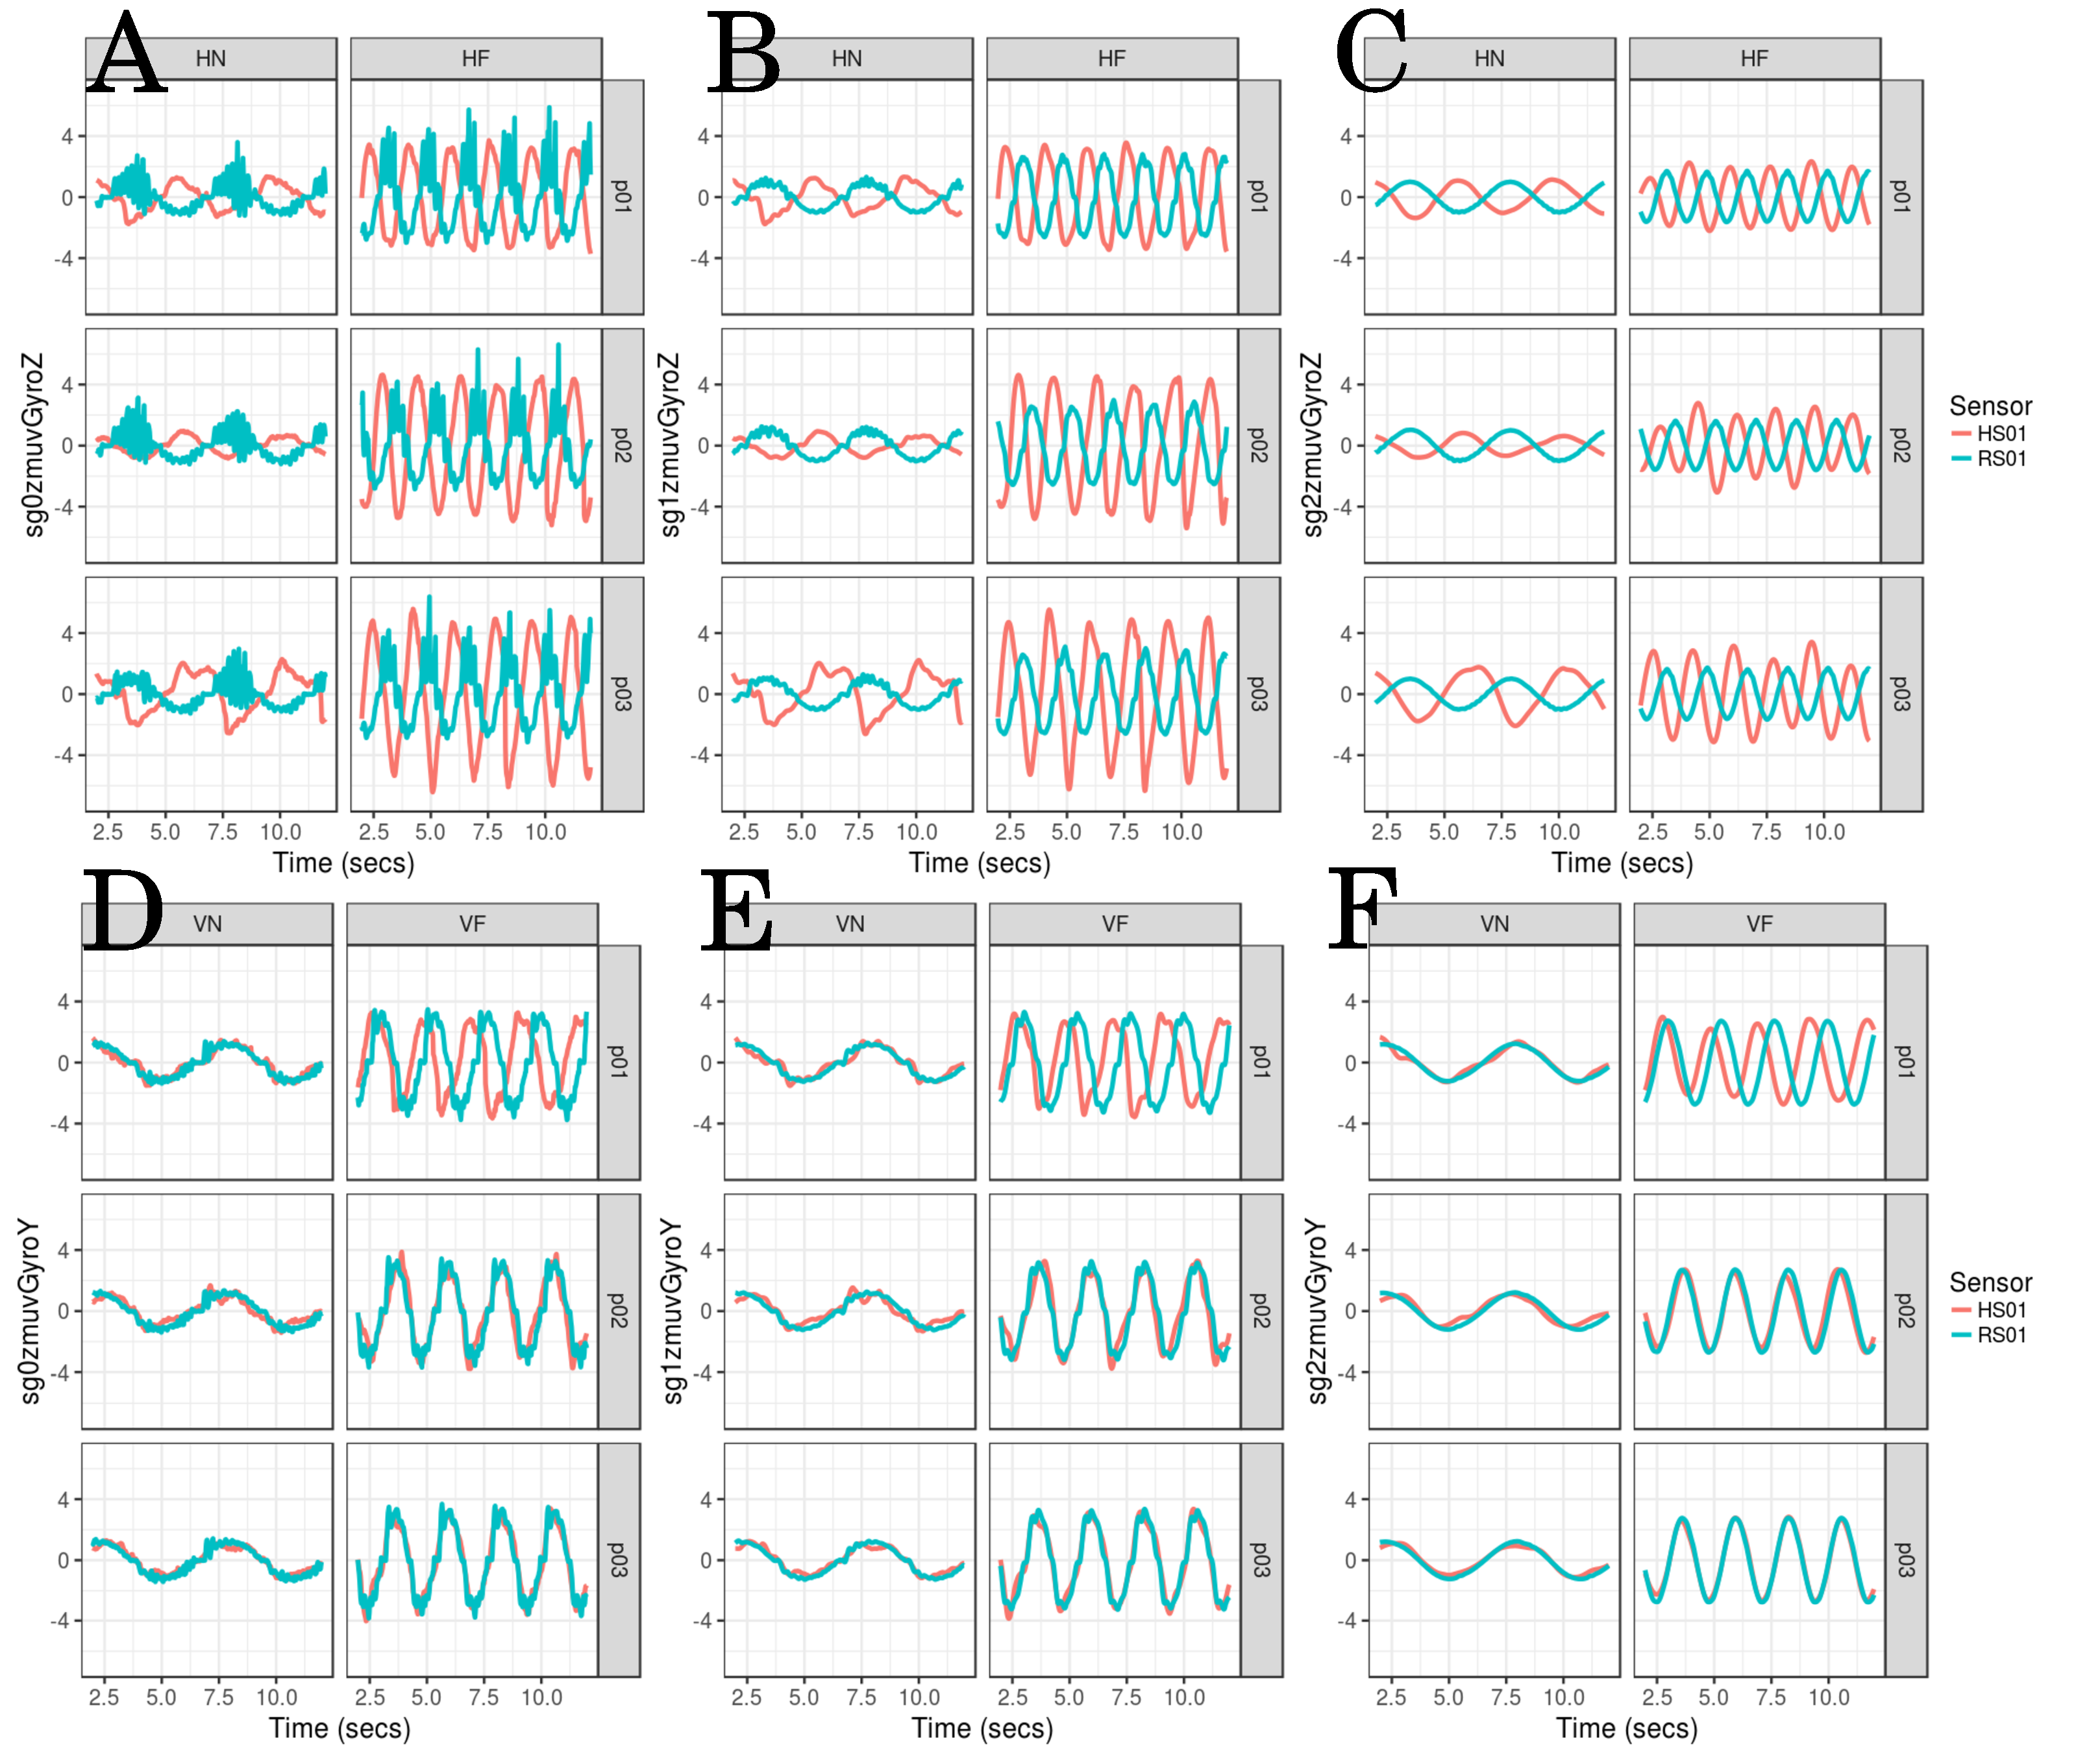
\includegraphics[width=1.0\textwidth]{fig-fig1.pdf}
    	\caption{ 
	{\bf Time series for horizontal and vertical arm movements.}
		(A/D) raw-normalised (sg0zmuv), 
		(B/E) normalised-smoothed 1 (sg1zmuv) and
		(C/F) normalised-smoothed 2 (sg2zmuv).
		Time series are only for three participants 
		($p01$, $p02$, and $p03$) 
		for horizontal and vertical arm movements in normal 
		and faster velocity (HN, HF, VN, VF) 
		with the normalised GyroZ or GyroY axis 
		and with one sensor attached to the participant (HS01) 
		and other sensor attached to the robot (RS01).	
	Code and data to reproduce the figure is available in \cite{srep2020}.
        }
    \label{fig:ts}
\end{figure}
%%---------------------------------(FIGURE)------------------------------------




\subsubsection*{Raw data}
%Considering the work of \cite{shoaib2016} which provided evidence of an 
%improvement in recognition activities when combining data from 
%accelerometer and gyroscope. 
We focus our analysis from data of the 
accelerometer and gyroscope of the NeMEMsi sensors \cite{Comotti2014} and 
leave the data of the magnetometer and quaternions for further investigation 
because of their possible variations with regard to magnetic disturbances \cite{shoaib2016}.
Data from the accelerometer is defined by triaxial time series 
$A_x(n)$, $A_y(n)$, $A_z(n)$ which forms the matrix $\boldsymbol{A}$ 
(Eq.~\ref{eq:AG}), and the same for data from the gyroscope 
which is defined by triaxial time-series of $G_x(n)$, $G_y(n)$, $G_z(n)$ 
representing the matrix $\boldsymbol{G}$ (Eq.~\ref{eq:AG}).
Both triaxial time series of each sensor, $a$ and $g$, are denoted with 
its respective axes subscripts $x,y,z$, where $n$ is the sample index 
and $N$ is the same maximum length of all axes for the time series.
%Matrices  $\boldsymbol{A}$ and $\boldsymbol{G}$ are represented as follows
%%---------------------------------(EQUATION)----------------------------------
\begin{equation}\label{eq:AG}
\boldsymbol{A} =
\begin{pmatrix}
  A_x(n) \\
  A_y(n) \\
  A_z(n)
\end{pmatrix}
=
\begin{pmatrix}
 a_x(1),a_x(2),\dots,a_x(N) \\
 a_y(1),a_y(2),\dots,a_y(N) \\
 a_z(1),a_z(2),\dots,a_z(N) 
\end{pmatrix},
%\end{equation}
%%---------------------------------(EQUATION)-----------------------------------
%and 
%%---------------------------------(EQUATION)-----------------------------------
%\begin{equation}\label{eq:G}
\boldsymbol{G} =
\begin{pmatrix}
 G_x(n) \\
 G_y(n) \\
 G_z(n)
\end{pmatrix}
=
\begin{pmatrix}
 g_x(1),g_x(2),\dots,g_x(N) \\
 g_y(1),g_y(2),\dots,g_y(N) \\
 g_z(1),g_z(2),\dots,g_z(N) 
\end{pmatrix}.
\end{equation}
%%---------------------------------(EQUATION)-----------------------------------


\subsubsection*{Postprocessing data}
After the collection of raw data from four NeMEMsi sensors,
time synchronisation alignment and interpolation were performed 
in order to create time series with the same length and synchronised time.
We refer the reader to \cite{Comotti2014} for further
details about the time synchronisation process.

\subsubsection*{Normalising data}
Data is normalised to be zero mean and unit variance.
The sample mean and sample standard deviation using $x(n)$ is given by
%%---------------------------------(EQUATION)----------------------------------
\begin{equation}\label{eq:ms}
\mu_{x(n)}= \frac{1}{N} ( \sum_{i=1}^N x(i) ), \quad 
	\sigma_{x(n)} =  \sqrt{ \frac{  \sum_{1=1}^N ( x(i) - \mu_{x(n)} )^2 }{ N-1 }  },      
\end{equation}
%%---------------------------------(EQUATION)----------------------------------
and the normalised data, $\hat{x}(n)$, is computed as follows
%%---------------------------------(EQUATION)----------------------------------
\begin{equation}\label{eq:normalization}
\hat{x} (n) = \frac{   x(n) -  \mu_{x(n)}  }{   \sigma_{x(n)} }.   
\end{equation}
%%---------------------------------(EQUATION)----------------------------------

\subsubsection*{Smoothing data}
Commonly, a low-pass filter is use either to capture the low 
frequencies that represent \%99 of the human body energy or to get 
the gravitational and body motion components of 
accelerations \cite{anguita2013}. However, the elimination of 
a range of frequencies is not the main focus of this work but 
the conservation of the structure of time series in terms of 
their width and heights where, for instance, Savitzky-Golay filter 
can be a way to accomplish such task \cite{press1992}. 
Savitzky-Golay filter is based on the 
principle of moving window averaging which preserves the area under 
the curve (the zeroth moment), its mean position in time 
(the first moment) but the line width (the second moment) is violated 
and that results, for example, in the case of spectrometric data, into
a narrow spectral line with reduced height and width. 
With that in mind, the aim of Savitzky-Golay filtering is to find filter 
coefficients $c_n$ that preserve higher momentums which are based on local 
least-square polynomial approximations \cite{savitzkygolay1964, 
press1992, schafer2011}.
Therefore, Savitzky-Golay coefficients are computed with \texttt{sgolay(p,n,m)} 
in R where \texttt{p} is the filter order, 
\texttt{n} is the filter length (must be odd) and \texttt{m} is the 
$m$-th derivative of the filter coefficients \cite{Rsignal}. 
Smoothed signal is represented with a tilde over the original 
variable of the signal: $\tilde{x}(n)$.

\subsubsection*{Windowing data size}
With regards to the window size, Shoaib et al. in 2016 \cite{shoaib2016} 
investigated effects of seven window lengths (2, 5, 10, 15, 20, 25, 30 seconds)
and combination of inertial sensors (accelerometer, gyroscope and linear 
acceleration sensor) to improve the activity recognition performance for 
repetitive activities (walking, jogging and biking) and less repetitive 
activities (smoking, eating, giving a talk or drinking a coffee).
With that in mind, Shoaib et al. \cite{shoaib2016} concluded that the 
increase of window length improve the recognition of complex activities 
because these requires a large window length to learn the repetitive 
motion patterns. Particularly, one of the recommendations is to use large 
window size to recognise less repetitive activities which mainly involve 
random hand gestures. Therefore, for the four activities 
(HN, HF, VN, and VF) in this work, which are mainly repetitive, 
we select only four window sizes for analysis: 2-s window (100 samples), 
5-s window (250 samples), 10-s (500 samples) and 15-s window (750 samples) 
(Fig~\ref{fig:sts}).

%*******************************************************************************
%*******************************************************************************
%*******************************************************************************
\section*{Results}

\subsection*{Reconstructed State Spaces}
As noted in the Introduction, a challenge in the implementation of uniform time-delay embedding 
arises from the selection of embedding parameters because of the uniqueness of each time series 
in terms of its structure (e.g., modulation of amplitude, frequency, phase etc.). 
With that in mind, the options are to either calculate embedding parameters for each unique 
instance (which can make comparison challenging) or to find parameters which can apply to all 
instances in the study.
We recognise that the latter approach is not without its problems, 
but our approach is to compute sample mean over all values in each of the conditions of the 
time series for minimum dimension and minimum delay values.

\subsubsection*{Minimum embedding parameters}
Minimum embedding parameters were initially computed using False Nearest Neighbour (FNN) 
and Average Mutual Information (AMI).   We used FNN to calculate a value for $m$
to unfold the attractors and AMI to calculate a value for $\tau$ and maxime the 
information in the unfolded attractor.
To illustrate this, figure \ref{fig:cao_ami} (A) show box plots for minimum embedding 
values for sensors on the wrist of the human (HS01) and the robot (RS01).   
As we had assumed, minimum embedding values for HS01 show greater variation than 
those for RS01 (as indicated by differences in interquartile ranges).  
Additionally, figure \ref{fig:cao_ami} (A) show a decrease in mean values (rhombus) in the box plots 
as smoothness of the time-series increases (see sg0, sg1, sg2).  
Figure \ref{fig:cao_ami} (B) show box plots for Average Mutual Information (AMI).  
One can see that, in contrast to RS01, minimum values for HS01 tend to spread 
as the smoothness of the time-series increases.
The sample mean for minimum value of embedding parameter, 
$m$ derived from FNN  (figures \ref{fig:cao_ami} A) is $\overline{m}_0=6$ 
and $\tau$ from AMI (figures \ref{fig:cao_ami} B) is $\overline{\tau}_0=8$.

%---------------------------------(FIGURE)-------------------------------------
\begin{figure}[ht]
\centering
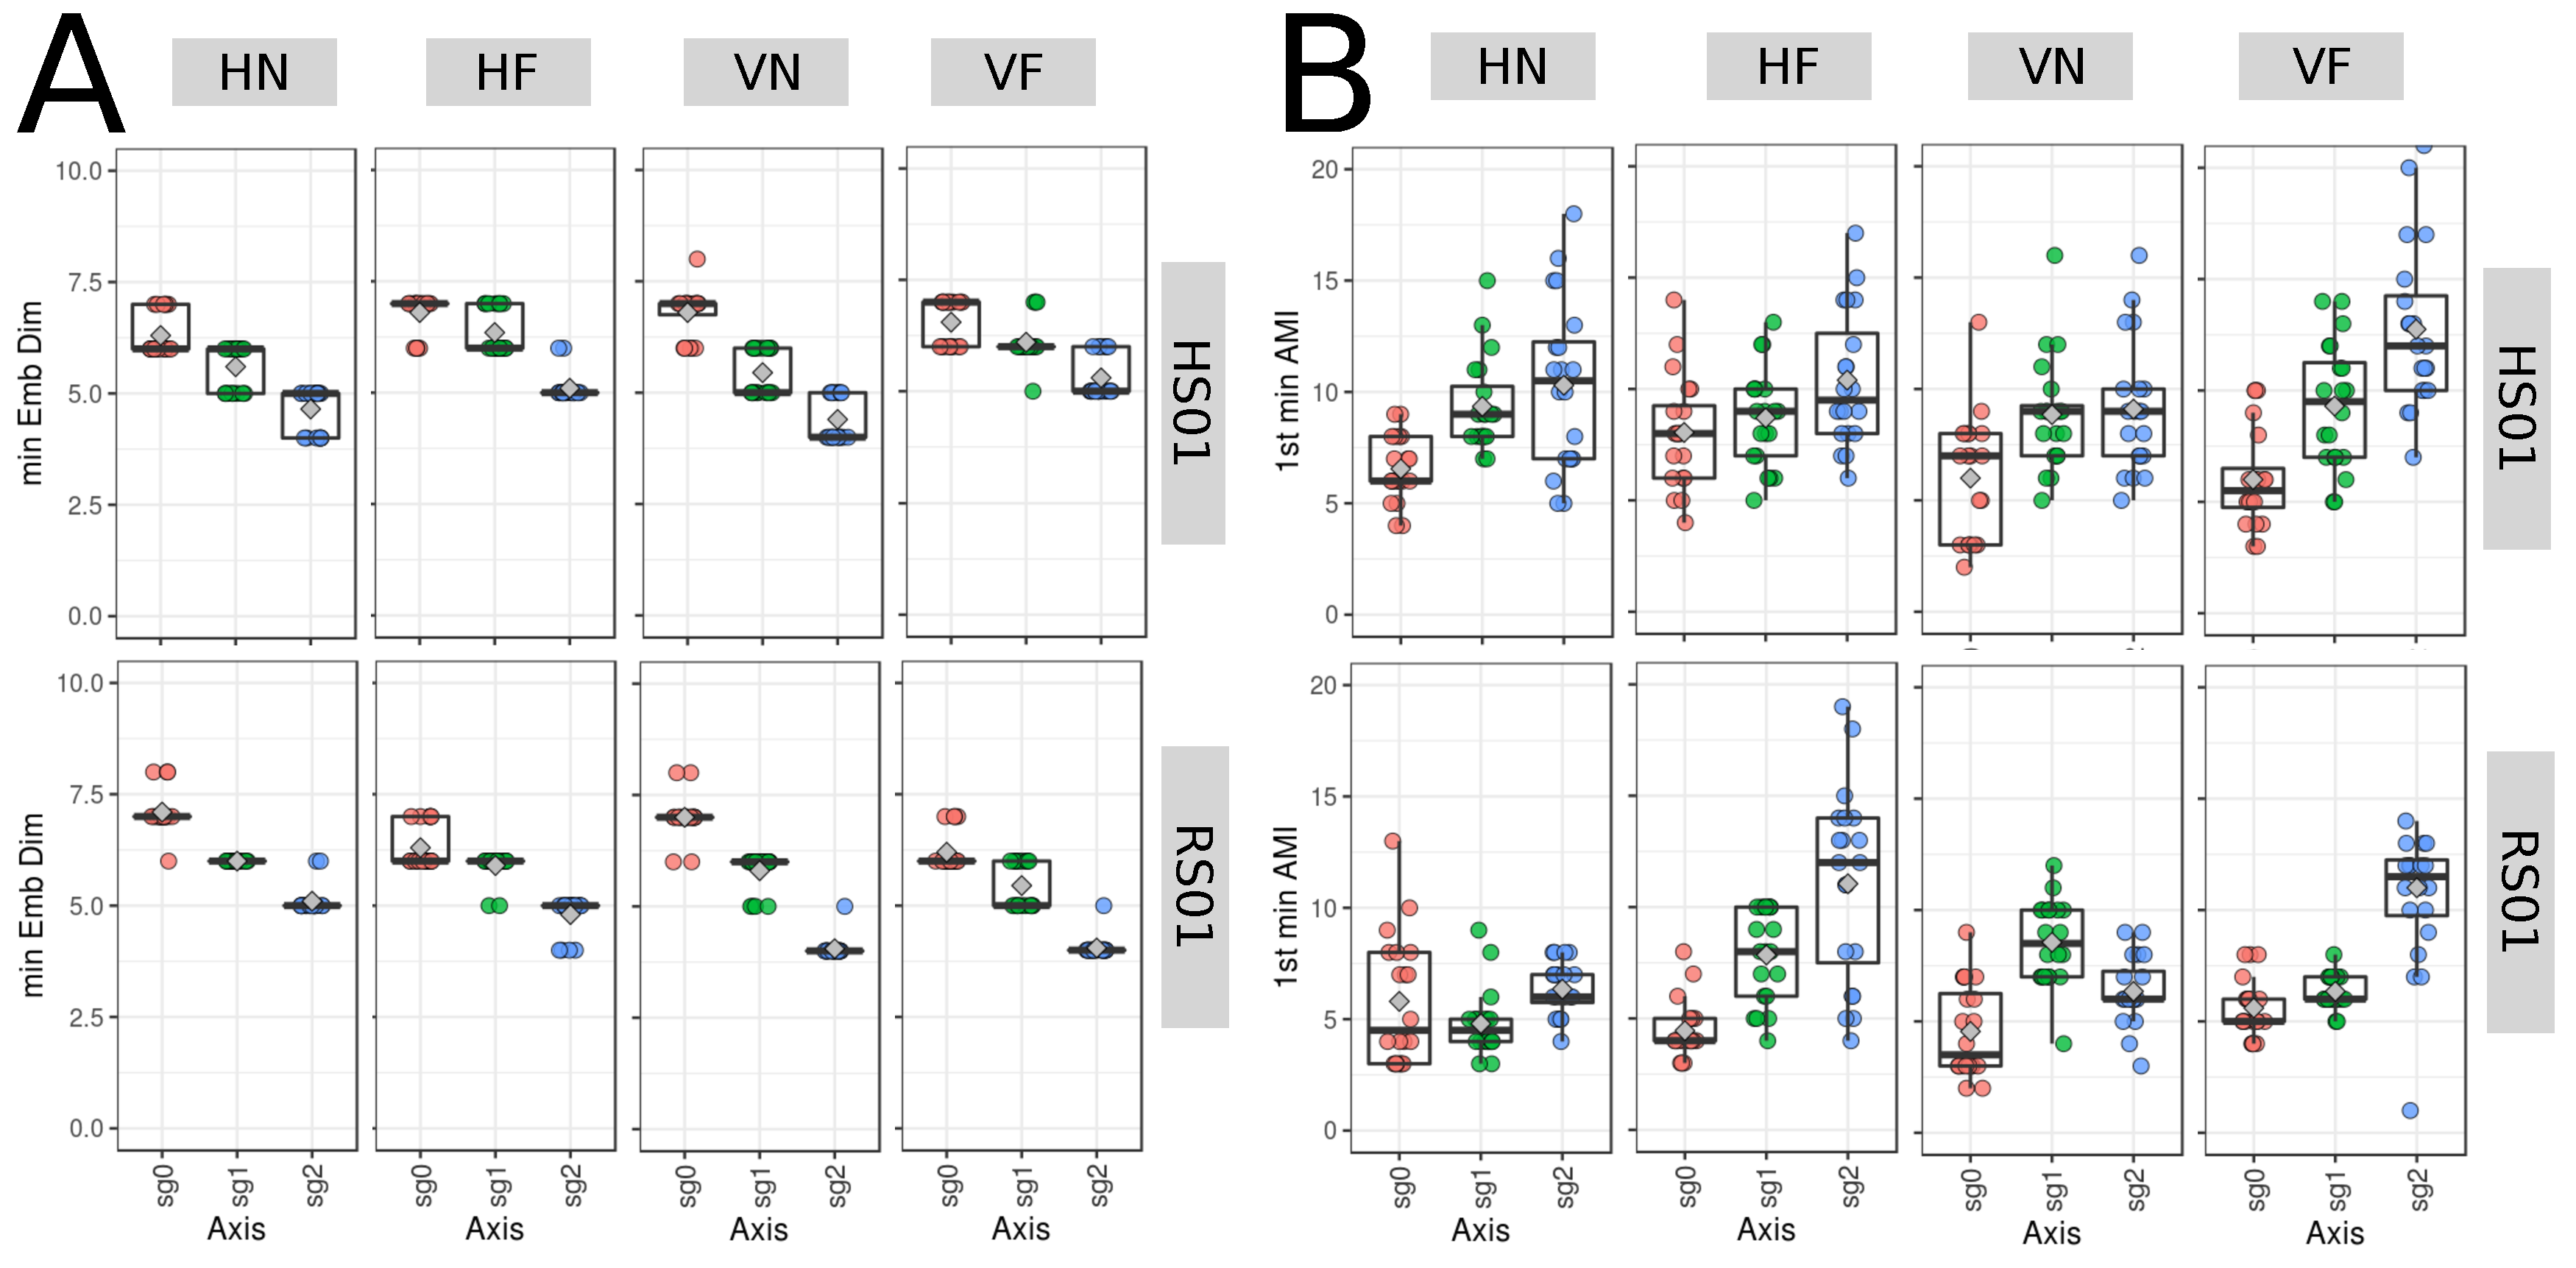
\includegraphics[width=1.0\textwidth]{fig-fig2.pdf}
	\caption{
	{\bf Box plots of minimum embedding parameters.} 
	Box plots of (A) minimum embedding dimensions 
	and (B) first minimum AMI values for 
	Horizontal Normal (HN), Horizontal Faster (HF),
	Vertical Normal (VN) and Vertical Faster (VF)
	with sensors attached to participants (HS01) and
	sensor attached to robot (RS01).
	Minimum embedding parameters are for twenty participants 
	($p01$ to $p20$) with three smoothed signals 
	(sg0: sg0zmuvGyroZ, sg1: sg1zmuvGyroZ and sg2: sg2zmuvGyroZ)
	and window length of 10-sec (500 samples).
	Code and data to reproduce the figure is available in \cite{srep2020}.
        }
    \label{fig:cao_ami}
\end{figure}
%%---------------------------------(FIGURE)------------------------------------

\subsubsection*{Uniform Time-Delay Embedding}
Using the overall embedding parameters ($\overline{m_0}=6$, $\overline{\tau_0}=8$), 
the first three axis of the rotated Principal Components Analysis (PCA) 
are shown for the reconstructed state spaces of horizontal (figures~\ref{fig:rsss}(A)) 
and vertical (figures~\ref{fig:rsss}(B)) arm movements. 
While visual inspection of these figures 
suggests differences in the trajectories of the reconstructed state spaces, 
we require an objective quantification to determine the extent of the differences.  
One approach could be use Euclidean distances from the origin for points in these 
trajectories, but this proved inconclusive and was not able to capture 
the dynamics of the trajectories. Consequently, we applied 
Recurrence Plots and Recurrence Quantification Analysis.
%%---------------------------------(FIGURE)-------------------------------------
\begin{figure}[ht]
\centering
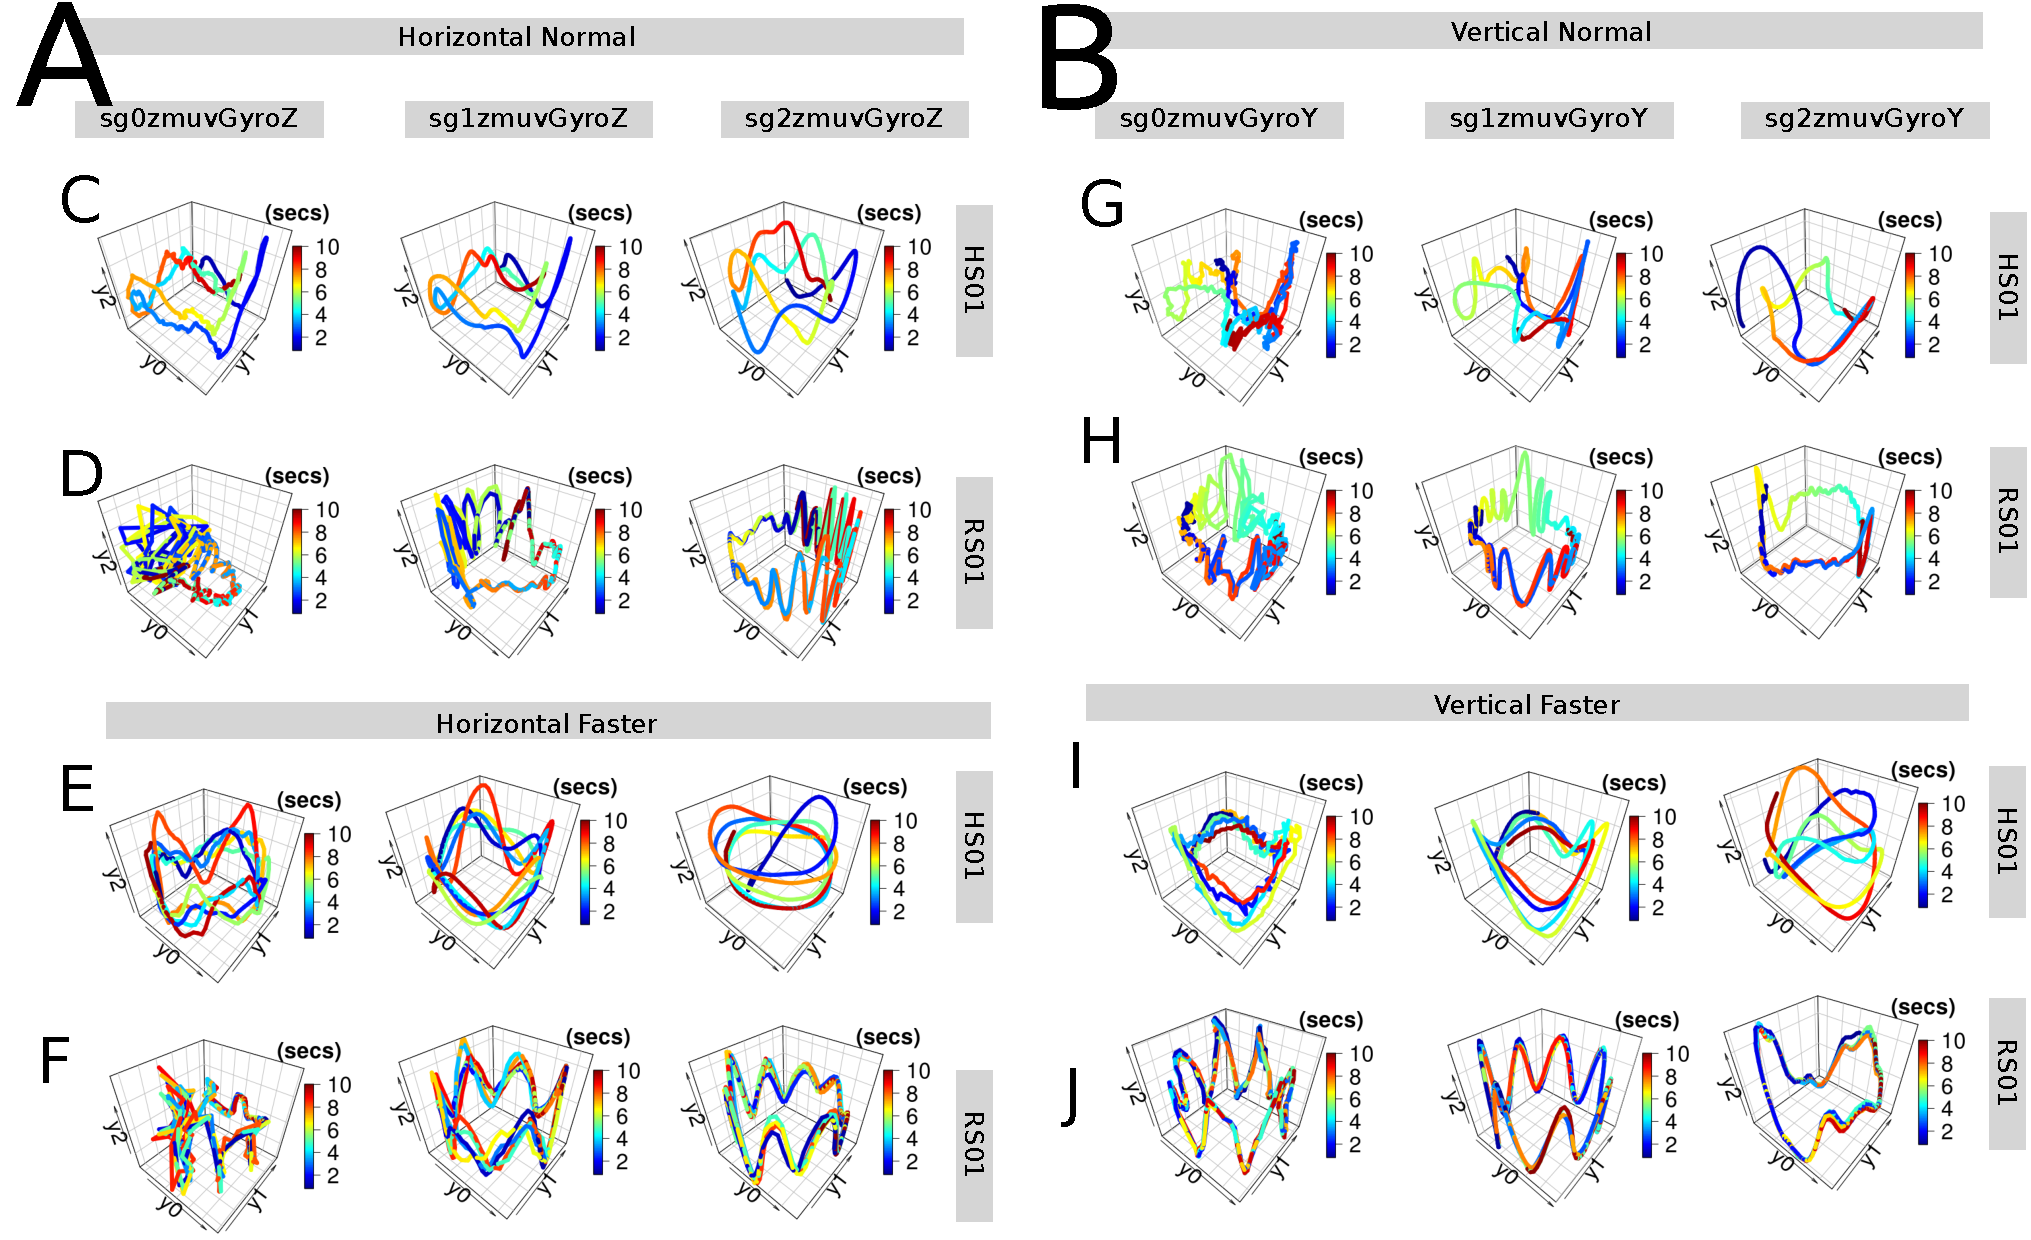
\includegraphics[width=1.0\textwidth]{fig-fig3.pdf}
\caption{
	{\bf RSSs for horizontal and vertical arm movements.}
	Reconstructed state spaces for time series for p01 of Figure \ref{fig:ts}.
	Reconstructed state spaces were computed with 
	embedding parameters 
	$\overline{m}_0=6$, $\overline{\tau}_0=8$
	for (A) horizontal and (B) vertical arm movements.
	Code and data to reproduce the figure is available in \cite{srep2020}.	
        }
    \label{fig:rsss}
\end{figure}
%%---------------------------------(FIGURE)------------------------------------



\subsection*{Recurrences Plots}
Using the average embedding parameters 
($\overline{m}_0=6$, $\overline{\tau}_0=8$) 
and an recurrence threshold of $\epsilon=1$.
As our interest is for dynamical transitions, 
there is little importance on the selection of $\epsilon$ which in this case
is 1. 
Recurrence Plots (RP) were computed for horizontal (figures~\ref{fig:rps}(A)) and 
vertical (figures~\ref{fig:rps}(B)) arm movements.
%%---------------------------------(FIGURE)-------------------------------------
\begin{figure}[ht]
\centering
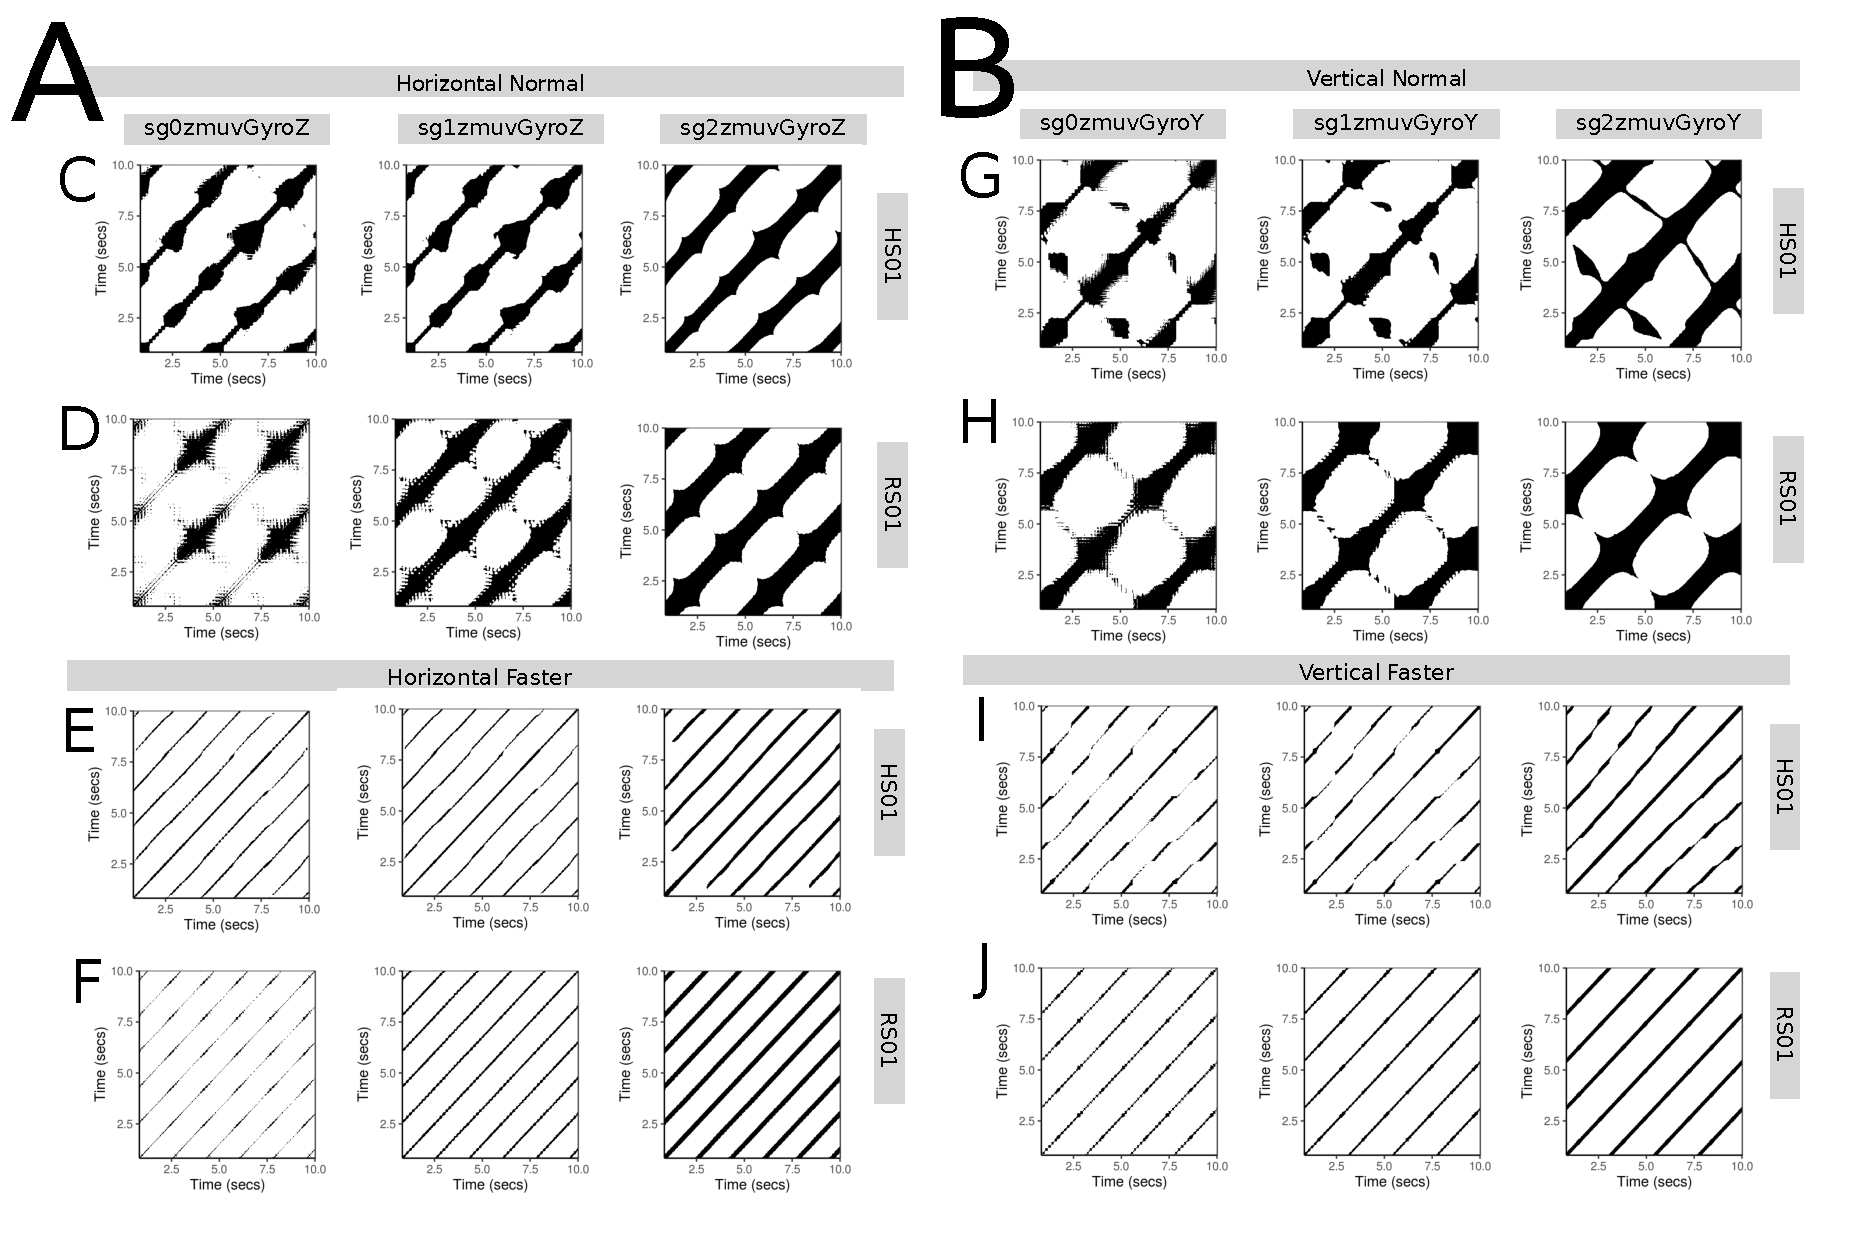
\includegraphics[width=1.0\textwidth]{fig-fig4.pdf}
\caption{
	{\bf RPs for horizontal (A) and vertical (B) arm movements.}	
	Recurrence plots were computed with 
	embedding parameters 
	$\overline{m}_0=6$, $\overline{\tau}_0=8$, and $\epsilon=1$.
	Code and data to reproduce the figure is available in \cite{srep2020}.
        }
    \label{fig:rps}
\end{figure}
%%---------------------------------(FIGURE)------------------------------------

\subsection*{Recurrence Quantification Analysis} \label{ch6:rqas}
Four Recurrence Quantification Analysis metrics (
percentage recurrence, REC, representing the percentage of black dots in RP; 
percentage determinism, DET, representing the predictability of the RP; 
ratio of DET / REC, RATIO; Shannon entropy, ENTR) 
were computed using the same parameters as for RP.
%\subsubsection*{REC values}
Figure~\ref{fig:RQABP}(A) presents box plots of REC values, 
for HS01, are more spread for Slow (i.e., 5 seconds per movement) movements 
in Horizontal (HS) or Vertical (VS) than for Fast (i.e., 2 seconds per movement).  
This suggests greater variation between participants for the Slow movements.  
For RS01, there is little variation between Slow and Fast movement
(interquartile range of 0.01). 
In terms of smoothness, there seems little effect of HS01 but RS01 values 
do show affects of smoothness (see the incremental changes of mean values (rhombus)).
%\subsubsection*{DET values}
Figure \ref{fig:RQABP}(B) presents DET values and shows 
little difference for type of movement or performer.  
However, DET values are affected by changes in smoothness of the signal, 
particularly for Fast movement.
%\subsubsection*{RATIO values}
Figure \ref{fig:RQABP}(C) presents the ratio of DET / REC. 
These values, for the human performer, vary less for HN than for HF movement.  
Additionally, smoothness leads to a decrease in mean values for Fast movements.
%\subsubsection*{ENTR values}
Figure \ref{fig:RQABP}(D) shows ENTR values are higher for the human 
performer than the robot, and vary with the smoothness of the time-series.
%%---------------------------------(FIGURE)-------------------------------------
\begin{figure}
\centering
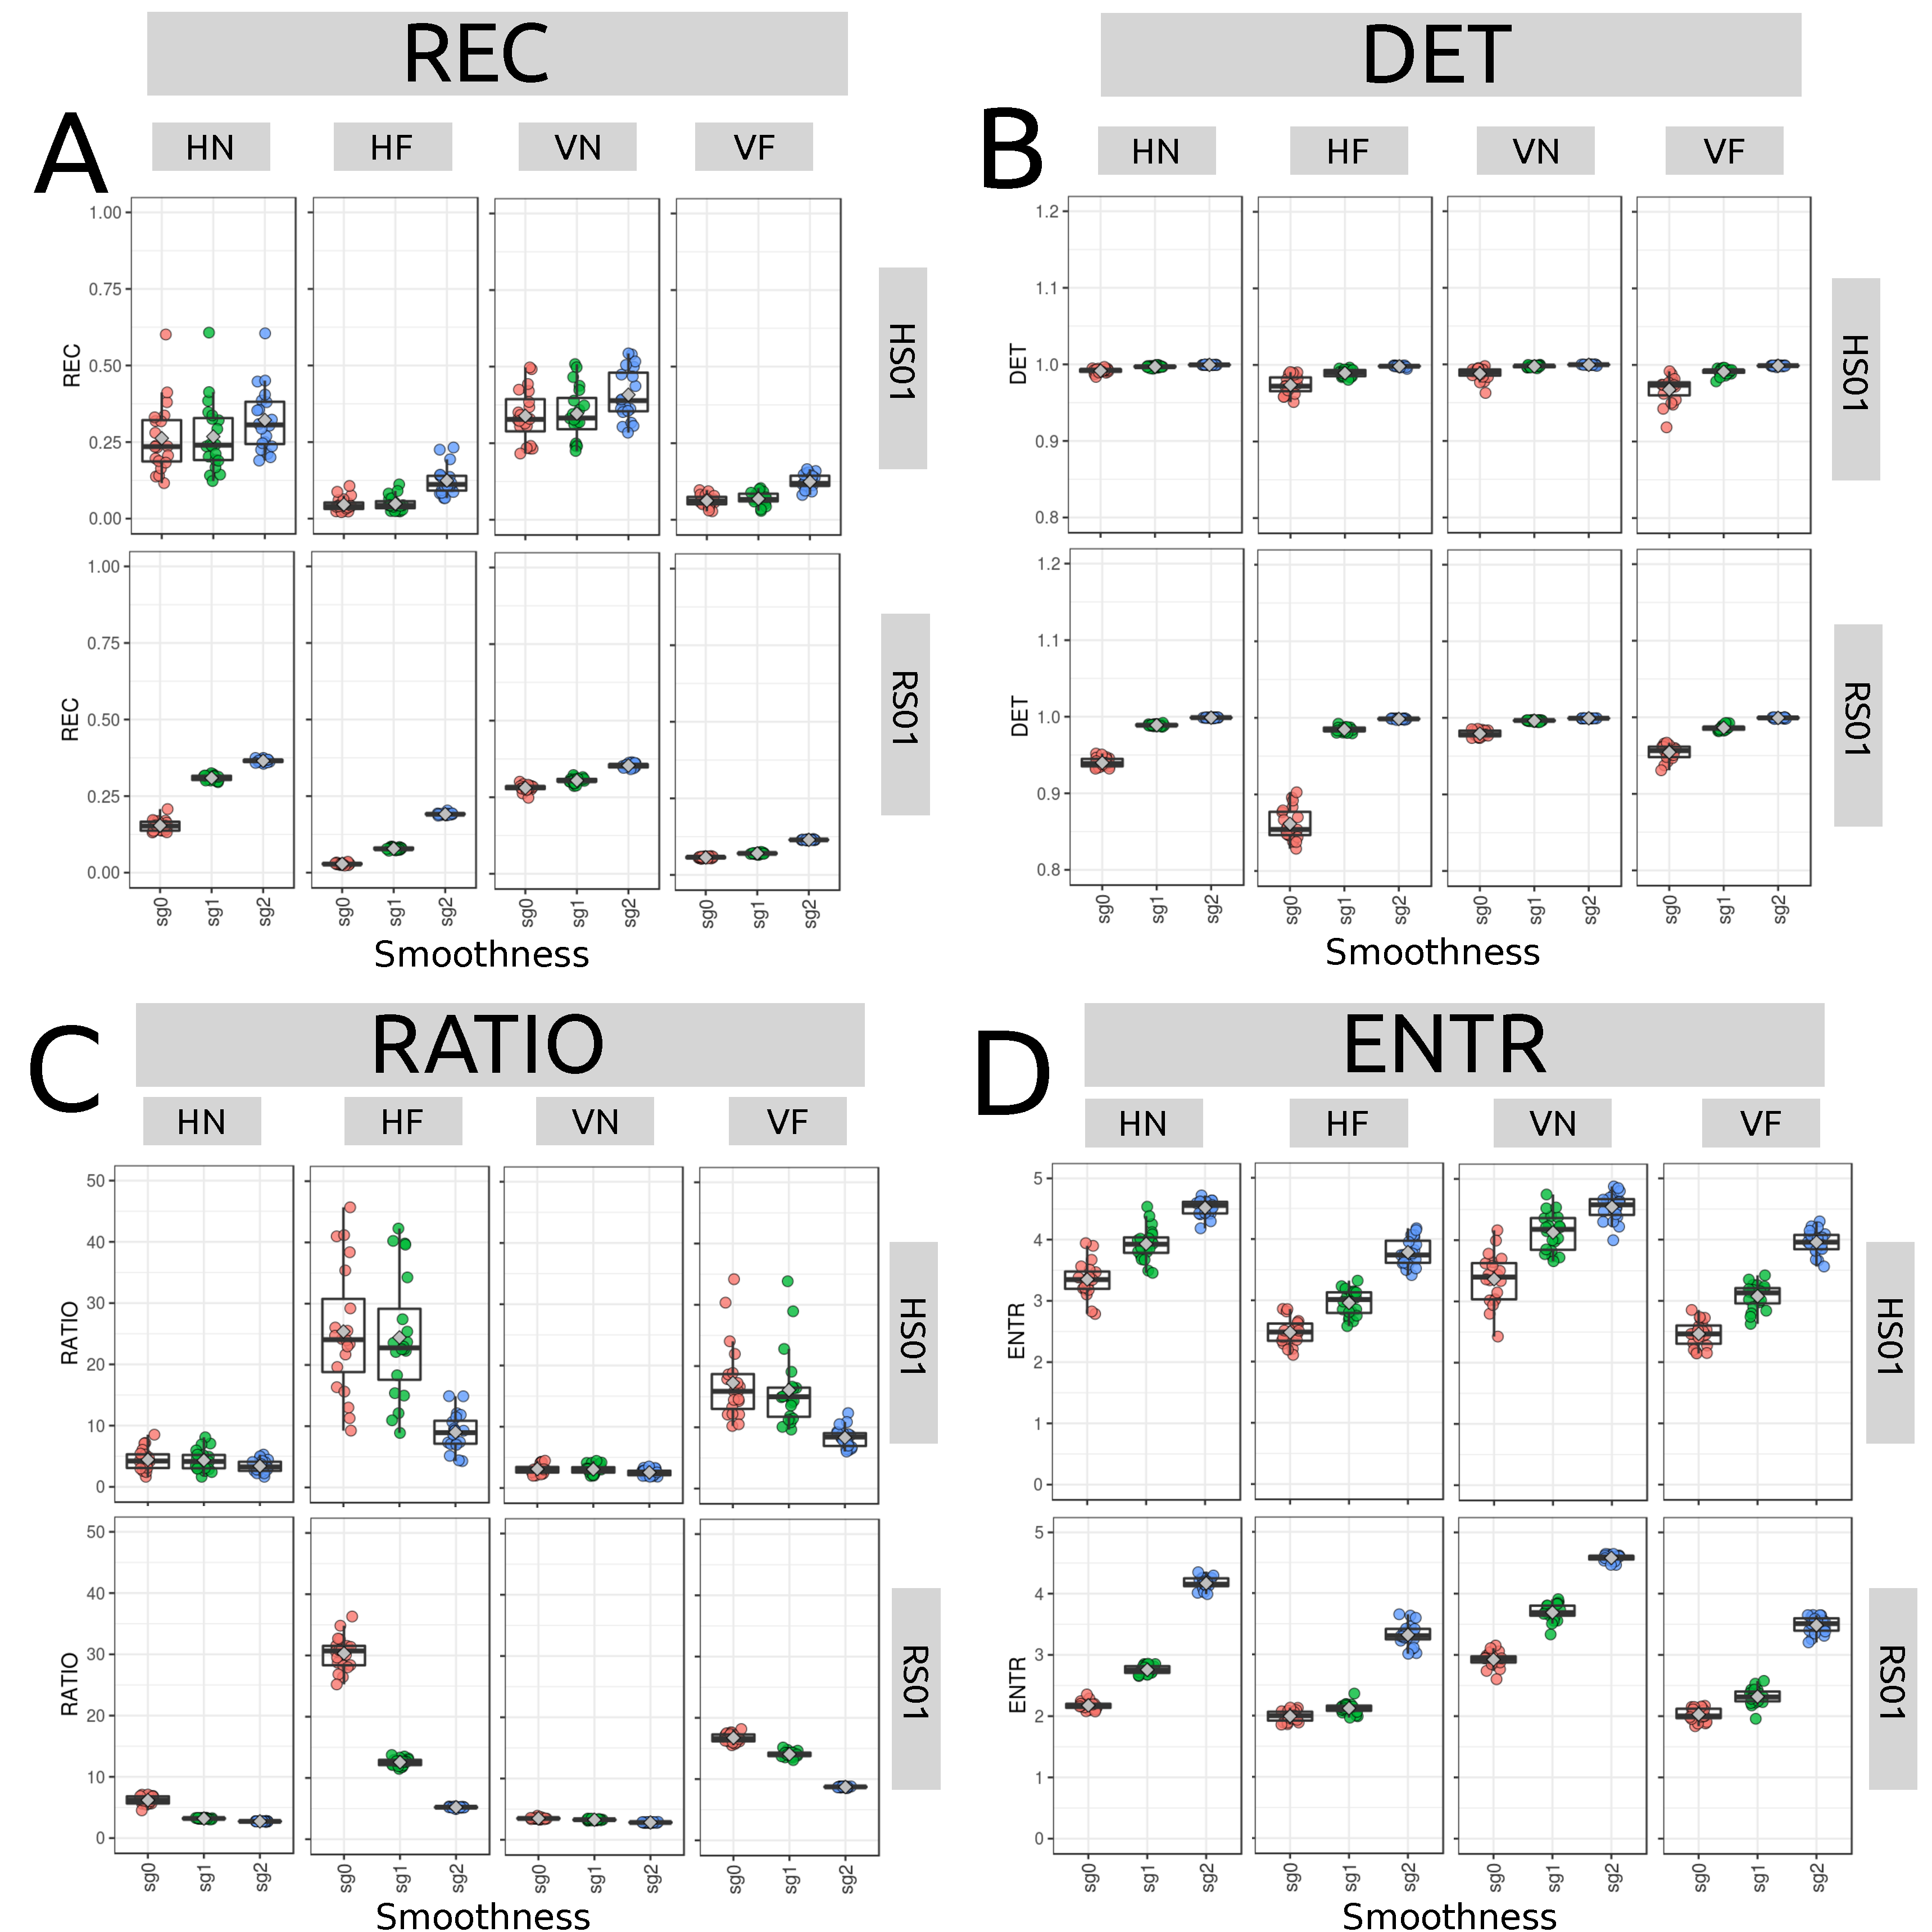
\includegraphics[width=1.0\textwidth]{fig-fig5.pdf}
    \caption
	[Box plots for RQA values]{
	{\bf Box plots for RQA metrics.}
	RQA metrics for (A) REC, (B) DET, (C) RATIO, and (D) ENTR of 
	20 participants performing HN, HF, VN and VF movements
	with sensors HS01, RS01 and three smoothed-normalised  
	time series (sg0, sg1 and sg2).
	RQA values were computed with 
	$\overline{m}_0=6$, $\overline{\tau}_0=8$, and $\epsilon=1$. 
	Code and data to reproduce the figure is available in \cite{srep2020}.
        }
    \label{fig:RQABP}
\end{figure}
%%---------------------------------(FIGURE)------------------------------------

%\subsection*{RQA metrics with fixed parameters}
%Considering that RQA metrics were computed with fixed embedding parameters 
%($m=6$ and $\tau=8$) and recurrence thresholds ($\epsilon=1$), we found 
%the following. REC values, which represents the \% of black points in the RPs, 
%were more affected with and increase in normal speed movements (HN and VN) 
%than faster movements (HF and VF) for the sensor attached to the participants 
%(HS01). Such decrease of REC values from normal speed to faster speed 
%movements is also presented in data from sensor attached to the robot (RS01), 
%and little can be said with regard to the dynamics of the time series coming 
%from RS01 (Fig \ref{fig:RQABP}A).
%Similarly, DET values, representing predictability and 
%organisation in the RPs, present little variation in the any of the time 
%series where little can be said (Fig \ref{fig:RQABP}B).
%In contrast, RATIO values, which represent 
%dynamic transitions, were more variable for faster movements (HF and VF) 
%than normal speed movements (HN and VN) with sensors attached to the 
%participants (HS01). For data coming from sensors attached to the robot 
%(RS01), RATIO values from horizontal movements (HN, HF) appear to vary 
%more than values coming from vertical movmentes (VN, VF) 
%(Fig \ref{fig:RQABP}C).
%With that, it can be said that RATIO values can represent a bit better
%than REC or DET metrics for the variability of imitation activities in 
%each of the conditions for time series.
%Similarly, ENTR values for HN were higher than values for HF
%and ENTR values varied more for sensor attached to participants 
%than ENTR values for sensors of the robot. It is evidently that 
%the higher the entropy the more complex the dynamics are, 
%however, ENTR values for HN appear a bit higher than HF values, 
%for which we believe this happens because of the structure the time series
%which appear more complex for HN than  HF movements which presented a 
%more consistence repetition (Fig \ref{fig:RQABP}D).


\subsection*{3D RQA ENTR}
As ENTR appeared to be have higher sensitivity than the other measures, 
we explored the impact of different embedding parameters 
$ \{ m \in \mathbb{R} | 1 \le m \le 10  \} $,
$  \{ \tau \in \mathbb{R} | 1 \le \tau \le 10  \} $ 
incrementing by 1 each run, with recurrence thresholds $\epsilon=1, 2, 3$ 
and levels of smoothness (sg0, sg1, sg2).  
Figure \ref{fig:RQA-IND} shows that increasing recurrence 
threshold leads to an increase in ENTR regardless of level of smoothness.  
Similarly, increasing level of smoothness will also increase ENTR (figure \ref{fig:RQA-IND}).
In terms of movement or performer, RQA ENTR decrease from Slow (HS, VS) to Fast (HF, VF) 
for both human (HS01) and (RS01) (Figures~\ref{fig:3dRQAENTR_sensoractivities}).
In terms of individual differences, for human participants, 
figure \ref{fig:3dRQAENTR_participantsactivities} compares p01, p02 and p03 (for illustrative purposes) --
both between each other and in comparison with the more consistent performance of the robot.  
In terms of window length (w100 (2s), w250 (5s), w500(10s), w750 (15s)), 
figure \ref{fig:3dRQAENTR_windowsactivities} shows that improvement in 
capture with number of samples, although this has less of an effect on RQA ENTR.

%%---------------------------------(FIGURE)-------------------------------------
\begin{figure}
\centering
\includegraphics[width=1.0\textwidth]{fig-rqa-epsilons.pdf}
    \caption
	[3D surface plots of RQA ENTR values]{
	{\bf 
	3D surface plots of RQA ENTR values for different recurrence threshold and smoothness levels.}
	RQA ENTR values are
	for embedding parameters
	$ \{ m \in \mathbb{R} | 0 \le m \le 10  \} $,
	$ \{ \tau \in \mathbb{R} | 0 \le \tau \le 10  \} $
	incrementing by one and three recurrence thresholds $\epsilon=1, 2, 3$.
	RQA ENTR values were computed with data from $p03$, sensor HS01, with 
	a window size of 10-secs (500 samples).
	Code and data to reproduce the figure is available in \cite{srep2020}.
        }
    \label{fig:RQA-IND}
\end{figure}
%%---------------------------------(FIGURE)------------------------------------

%%---------------------------------(FIGURE)-------------------------------------
\begin{figure}[ht]
\centering
\includegraphics[width=1.0\textwidth]{fig-rqa-sensors-activities.pdf}
    \caption{
	{\bf 3D surface plots of RQA ENTR values for different sensors and activities.}
	RQA ENTR values are for embedding parameters
	$ \{ m \in \mathbb{R} | 0 \le m \le 10  \}$,
	$ \{ \tau \in \mathbb{R} | 0 \le \tau \le 10  \}$
	with $\epsilon = 1 $ considering four activities 
	Horizontal Normal (HN), Horizontal Faster(HF), Vertical Normal(VN), and 
	Vertical Faster (VF) and sensors Human Sensor 01 (HS01) and 
	Robot Sensor (RS01).
	RQA ENTR values were computed from data of $p03$, sg0 and 
	window size of 10-secs (500 samples).
	Code and data to reproduce the figure is available in \cite{srep2020}.
       }
\label{fig:3dRQAENTR_sensoractivities}
\end{figure}
%%---------------------------------(FIGURE)-------------------------------------

%%---------------------------------(FIGURE)-------------------------------------
\begin{figure}[ht]
\centering
\includegraphics[width=0.9\textwidth]{fig-rqa-participants.pdf}
    \caption{
	{\bf 3D surface plots of RQA ENTR values for different participants, activities and sensors.}
	RQA ENTR values are for participants (p01, p02, and p03) 
	in the categories of 
	(A) Human Sensor 01 (HS01) and 
	(B) Robot Sensor 01 (RS01)
	considering embedding parameters
	$ \{ m \in \mathbb{R} | 0 \le m \le 10  \}$,
	$ \{ \tau \in \mathbb{R} | 0 \le \tau \le 10  \}$
	with $\epsilon = 1$ and four activities 
	Horizontal Normal (HN), Horizontal Faster(HF), Vertical Normal(VN), and 
	Vertical Faster (VF).
	RQA ENTR values were computed from data of sg0 and window size of 10-secs (500 samples).
	Code and data to reproduce the figure is available in \cite{srep2020}.
       }
\label{fig:3dRQAENTR_participantsactivities}
\end{figure}
%%---------------------------------(FIGURE)-------------------------------------

%%---------------------------------(FIGURE)-------------------------------------
\begin{figure}[ht]
\centering
\includegraphics[width=1.0\textwidth]{fig-rqa-windows}
    \caption{
	{\bf 3D surface plots of RQA ENTR values for different windows lengths and activities.}
	RQA ENTR values are for embedding parameters
	$ \{ m \in \mathbb{R} | 0 \le m \le 10  \}$,
	$ \{ \tau \in \mathbb{R} | 0 \le \tau \le 10  \}$, 
	with $\epsilon = 1 $ considering four 
	windows lengths (e.g., w100 (100 samples), w250 (250 samples),
	w500 (500 samples) and w750 (750 samples)) and
	four activities 
	Horizontal Normal (HN), Horizontal Faster(HF), Vertical Normal(VN), and 
	Vertical Faster (VF).
	RQA ENTR values were computed from data of $p01$ and sg0.
	Code and data to reproduce the figure is available in \cite{srep2020}.
       }
\label{fig:3dRQAENTR_windowsactivities}
\end{figure}
%%---------------------------------(FIGURE)-------------------------------------

To summarise this section of results, it can be said that computing
embedding parameters for individual structure of time-series 
data is already a solved problem \cite{frank2010, sama2013, bradley2015}. 
However, it has been shown the challenge of finding embedding parameters
for nonlinear dynamic tools that represent a set of different time-series data.
That said, we proposed the use of sample mean of the set of embedding parameters
for RSSs, RP and RQA to then noticed that the selection of recurrence 
threshold, $\epsilon$, is also an open problem.
For which, this work proposed the variation of recurrence thresholds 
and embedding parameters to show the relationships of these to different datasets 
(participants, activities, windows lengths and sensors).

%*******************************************************************************
%*******************************************************************************
%*******************************************************************************
\section*{Discussion}
While there are many approaches to estimating embedding parameters for nonlinear analysis, 
these can be influenced by the structure of the time-series data.   
We show that, for RSS, RP and RQA, the estimation of embedding parameters can be performed 
using a sample mean which, together with recurrence threshold, can be shown to be 
influenced by activity, performer, window length and smoothness of time-series.  
It is known that time-series from different sources and with different characteristics 
require different embedding parameters, and this can produce different RSS, RPs and RQAs. 
Although this work helps to understand the open problem of 
finding right balance among (i) the level of smoothness of the signal, 
(ii) the selection of recurrence thresholds and (iii) 
the range of embedding parameters, 
we have shown how RQA metrics can help to quantify movement variability.

\section*{Conclusions}
In this paper we show how the selection of nonlinear analysis tool  
(i.e., RSS, RP, RQA metrics) depends on what question one wishes to 
address with time-series data (e.g., predictability, organisation, dynamics, complexity).  
Time-series data characteristics (e.g., window length, smoothness), 
time-series structure (e.g., frequency, amplitude) and 
data source (e.g., sensor placement, performance, movement) all influence 
the results that nonlinear analysis methods can provide.
That said, it has been shown that the use of different characteristics of the data and 
their collection can help us visualise and quantify variability of movement using 
methods of nonlinear analysis.   
There remain limitations of nonlinear methods in 
relation to the estimation of parameters (e.g., recurrence threshold, embedding parameters) 
which reflect the dynamics of specific movement and performers, window length 
and structure of the time-series. 
We note that RQA DET seems to show low sensitivity 
to these differences, whereas REC and RATIO (primarily as a result of REC) show 
variation across performers and movements.   
RQA ENTR, with different recurrence thresholds, 
can quantify variation in the time-series data and offers the most appropriate means 
for analysing variability in movement to allow us to analyse individual differences 
between human performers.  
To then found out that RQA ENTR values with different recurrence 
thresholds were appropriate to quantify 
the different changes and variations of the characteristics of 
time-series data.
Therefore, the use of Shannon Entropy could be applied 
to analyse human participants who might vary in age, 
state of health, anthropometric features and capability to perform movement.

%% As a guideline references should be limited to 60 (this is not 
%% strictly enforced).
%\bibliography{sample}
%\bibliography{../references/references}
%\bibliography{references}
%*******************************************************************************
\documentclass[fleqn,10pt]{wlscirep}
\usepackage[utf8]{inputenc}
\usepackage[T1]{fontenc}
%\graphicspath{{../}} %goes to path: docs/

\title{Nonlinear methods to quantify Movement Variability in Human-Humanoid Interaction Activities}
\author[1,*]{Miguel Xochicale}
\author[2]{Chris Baber}
\affil[1]{King's College London, 
	School of Biomedical Engineering amd Imaging Sciences,
	London, SE1 7EU, UK
	} 
\affil[2]{University of Birmingham,
	School of Computer Science,
	Birmingham, 
	B15 2TT, 
	UK}
\affil[*]{miguel.xochicale@kcl.ac.uk}


%\keywords{Keyword1, Keyword2, Keyword3}

\begin{abstract}
Human movement variability arises from the process of 
mastering redundant (bio)mechanical degrees of freedom (DOF)
to successfully accomplish any given motor task
(from the most complex to even the simplest one) 
where flexibility and stability of many possible joint 
combinations helps to adapt to environment conditions. 
While the analysis of movement of variability is becoming increasingly 
popular as a diagnostic tool or skill performance evaluation, 
there are remain challenges in terms of defining 
the most appropriate methods and parameters to apply. 
For this work, we therefore investigate nonlinear dynamics methods 
such as reconstructed state space (RSSs), uniform time-delay embedding, 
recurrence plots (RPs) and recurrence quantification analysis metrics (RQAs)
with real-world time-series data of wearable inertial sensors. 
That said, twenty right-handed healthy participants 
imitated simple vertical and horizontal arm movements in normal 
and faster velocity from an humanoid robot.
We applied nonlinear methods to four activities, 
four window lengths and three levels of smoothed time-series data,
to then found visual differences in the patterns of RSSs and RPs
and statistical differences with RQA metrics.
We therefore conclude that Shannon Entropy for RQA is a robust method 
that help us to quantify activities, types of sensors, windows lengths 
and level of smoothness.
Hence this work might enhance the development of 
better diagnostic tools for applications in 
rehabilitation and sport science for skill performance
or new forms of human-humanoid interaction for
quantification of movement adaptations and motor pathologies.
\end{abstract}


\begin{document}
\flushbottom
\maketitle
\thispagestyle{empty}

\section*{Introduction}
The complexity of human movement arises from the process of mastering 
redundant (bio)mechanical degrees of freedom (DOF) to successfully 
accomplish any given motor task (Bernstein, 1967).
Such DOF are independent coordinates to uniquely 
describe the configurations of the system which provides flexibility 
and stability to adapt to a change environment conditions but 
that leads many possible combinations (Newell and Vaillancourt, 2001).
Hence, human movement complexity can be seen as a balance 
between the required DOF "to generate a stable (persistent) 
and flexible (variable) behavioural output in response to 
changing intentions and dynamic environmental
conditions" \cite{davids2003}. 
Consequently, one can see much variability in human movement even in the 
simplest of movements.  
While the analysis of movement of variability is becoming increasingly 
popular as a diagnostic tool or skill performance evaluation, 
there remain challenges in terms of defining 
the most appropriate methods and parameters to apply. 
In part, 
these challenges stem from the fact that the identification movement 
variability requires analysis of signals which are time-series of 
of $1-$dimension in $\mathbb{R}$ which are 
noisy, nonlinear and non-stationary \cite{gomezgarcia2014}.
Further problems arise from assigning a plausible locus of control to 
the movements, e.g., in order to determine whether variability is the 
result of deliberative control by the performer or whether it arises 
from exogenous or endogenous disturbances.  For this paper, our focus 
is on the analysis of signals; specifically, in terms of objectively 
quantifying variability of lower dimension signals using time-series analysis.

Methods for nonlinear time series analysis generally involve the estimation of the 
embedding parameters ($m$ embedding dimension and $\tau$ embedding delay) to 
reconstruct the state space,
where an $n$-dimensional is reconstructed state space using $1-$dimensional 
time series \cite{Quintana-Duque2012, Quintana-Duque2016, sama2013, 
frank2010, gomezgarcia2014, marwan2011, stergiou2011}.
Key to the selection of these parameters is the need to preserve 
topological properties of an unknown $M$-dimensional state space \cite{takens1981}.
An common approach to the construction of these state spaces 
involves Recurrence Plots (RPs), a graphical representation of black and white dots, 
which shows recurrent patterns of a $n$-dimensional system.
While RPs provide a human
interpretable picture of the system, these require further
analysis to allow the properties of that system to be quantified,
and so Recurrence Quantification Analysis (RQA) can be applied.
However, the estimation of the embedding parameters for
RQA remains an open problem (Bradley et al. 2015 \cite{bradley2015})
There is no agreed method to estimate embedding parameters
for RQA and other nonlinear methods \cite{bradley2015} 
because time series are system-dependent, i.e., these rely
on the initial conditions, and on the configuration and behaviour of the system.  
This means that, unless one holds all of the influencing 
variables constant, embedding parameters computed for one 
instance may not apply to another instance.   

One could apply methods, such as autocorrelation, mutual information, 
nearest neighbour (and we will apply these in this paper), 
but these methods assume that the data are well sampled, with 
little noise and (usually) that the signals are purely deterministic \cite{garland2016, kantz2003}.
That said, these methods can break-down in the face of real-world datasets 
which could have 
different length, 
different values of accuracy and precision (rounding errors due to finite 
precision of the measurement apparatus which include frequency 
acquisition \cite{frank2010}), or 
different levels of contamination from exogenous and endogenous 
sources of ‘noise’ \cite{garland2016}.  What is, perhaps, surprising is that 
even subject to these problems, the methods are useful and 
nonlinear dynamics approaches continue to tell us much about 
human movement \cite{Quintana-Duque2012, Quintana-Duque2016, sama2013, frank2010,
gomezgarcia2014, marwan2011, stergiou2011, bradley2015}.

For this paper, we explore the role of RPs and RQA in the 
analysis of simple human movement. 
We compare horizontal and 
vertical arm movements performed by neurotypical participants 
who are copying these movements being made by a humanoid robot.  
This provides an initial point of comparison 
(between human movement, which we assume to have a degree of variability, 
and the robot, which we assume to have a degree of consistency).   
Additionally, our interest lies in the estimation of embedding parameters 
in light of different features of the data, e.g., levels of smoothing, 
window length, structure of time-series based on movement, 
types of sensors, individual differences between participants and 
the movements that they perform. 
Specifically, we ask what are 
the effects of different embedding parameters, recurrence thresholds 
and characteristics of time-series on nonlinear analysis 
methods (i.e., reconstructed state space with 
uniform time-delay embedding, RPs and RQA)?



%*******************************************************************************
%*******************************************************************************
%*******************************************************************************
\section*{Methods}
\subsection*{State Space Reconstruction}
The method of state space reconstruction \cite{packard1980} 
\cite{takens1981} has been applied in many disciplines 
\cite{aguirre2009, stergiou2011, frank2010, 
sama2013, Quintana-Duque2016}. The method of state space reconstruction is 
based on uniform time-delay embedding methodology which is a simple 
matrix implementation that can reconstruct an unknown $d-$dimensional 
manifold $M$ from a scalar time series (e.g. one-dimensional 
time series in $\mathbb{R}$). A manifold, in this context, is a 
multidimensional curved surface within a space (e.g. a saddle) 
\cite{guastello-gregson2011}.

The use of a scalar time series is the main advantage of the method of state 
space reconstruction which in essence preserve dynamic invariants such as 
correlation dimension, fractal dimension, Lyapunov exponents, Kolmogorov-Sinai 
entropy and detrended fluctuation analysis \cite{bradley2015, 
Quintana-Duque2012, Quintana-Duque2013, Quintana-Duque2016, krakovska2015}.
However, selecting appropriate embedding parameters which are sued to apply the 
state space reconstruction is still an open challenge for which we present 
introductions for the methodologies to compute such embedding parameters 
With that in mind, in the following subsections, we describe in more detail 
the state space reconstruction theorem (RSSs), uniform time-delay embedding 
theorem (UTDE), false nearest neighbours (FNN) and average mutual 
information (AMI). 
%and other methodologies for state space reconstruction.

\subsection*{State Space Reconstruction Theorem}
Following the notation employed in \cite{casdagli1991, garland2016, gibson1992,
uzal2011, uzal2010, takens1981}, state space reconstruction is defined by:
%%********************************[EQUATION]************************************
\begin{equation}\label{eq:ssr}
  s(t)=f^t [s(0)],
\end{equation}
%%********************************[EQUATION]************************************
where $s$, $s: A \rightarrow M$ given that $A \subseteq \mathbb{R}$ and 
$M \subseteq \mathbb{R}^d$, represents a trajectory which evolves in an 
unknown $d-$dimensional manifold $M$, $f: M \rightarrow M$ is an evolution 
function and $f^t$, with time evolution $t \in \mathbb{N}$, is the $t$-th 
iteration of $f$ that corresponds to an initial position 
$s(0) \in M $ \cite{takens1981}.
%$f$ is a smooth dynamical system, where smooth means a 
%continuously differentiable system
%(e.g. derivatives exist at all points) \cite{guastello-gregson2011}.
Then, a point of a one-dimensional time series $x(t)$ in $\mathbb{R}$, 
can be obtained with
%%********************************[EQUATION]************************************
\begin{equation}\label{eq:measurement}
  x(t)=h[s(t)],
\end{equation}
%%********************************[EQUATION]************************************
where $h$ is a function, $h: M \rightarrow \mathbb{R}$, defined on the trajectory $s(t)$.
Reconstructed state space can then be described as an $n-$dimensional state 
space defined by $y(t)=\Psi[\boldsymbol{X}(t)]$ where 
$\boldsymbol{X}(t) = \{ x(t), x(t-\tau) , ...,x(t - (m-1)\tau  ) \}$ 
is the uniform time-delay embedding with a dimension embedding $m$
and delay embedding $\tau$ and
$ \Psi: \mathbb{R}^m \rightarrow \mathbb{R}^n$ is a further transformation
of dimensionality (e.g. Principal Component Analysis, 
Singular Value Decomposition, etc) being $n \leq m$.
With that in mind, uniform time-delay embedding, $\boldsymbol{X}(t)$, 
defines a map $\Phi: M \rightarrow \mathbb{R}^m$ such that 
$\boldsymbol{X}(t) = \Phi(s(t))$,
where $\Phi$ is a diffeomorphic map \cite{takens1981}
whenever $\tau > 0$ and $m > 2d_{box}$ and $d_{box}$ is the box-counting
dimension of $M$ \cite{garland2016}.
% "Given two manifolds $M$ and $N$, a differientiable map $f: M \rightarrow N$
% is called diffeomorphic if it is one-to-one correspondence and its inverse
% $f^{-1}: N \rightarrow M$ is differientiable as well \cite{wiki:diffeomorphic}".
Then, if $\Phi$ is an embedding of evolving trajectories in the reconstructed 
space then a composition of functions represented with $F^t$ is induced on the
reconstructed state space determined:
%by true smooth dynamical system $f^t$ and $\Phi$:
%********************************[EQUATION]************************************
\begin{equation}\label{eq:st}
  \boldsymbol{X}(t)=F^t [\boldsymbol{X}(0)] = \Phi \circ f^t \circ \Phi ^{-1}[\boldsymbol{X}(0)].
\end{equation}
%%********************************[EQUATION]************************************
With this in mind, an embedding is defined as "a smooth one-to-one 
coordinate transformation with a smooth inverse" and the total reconstruction 
map is defined as $ \Xi = \Psi \circ \Phi $ \cite{casdagli1991}.
Fig~\ref{fig:ssr} illustrates the state space reconstruction.
%%---------------------------------(FIGURE)-------------------------------------
\begin{figure}[ht]
\centering
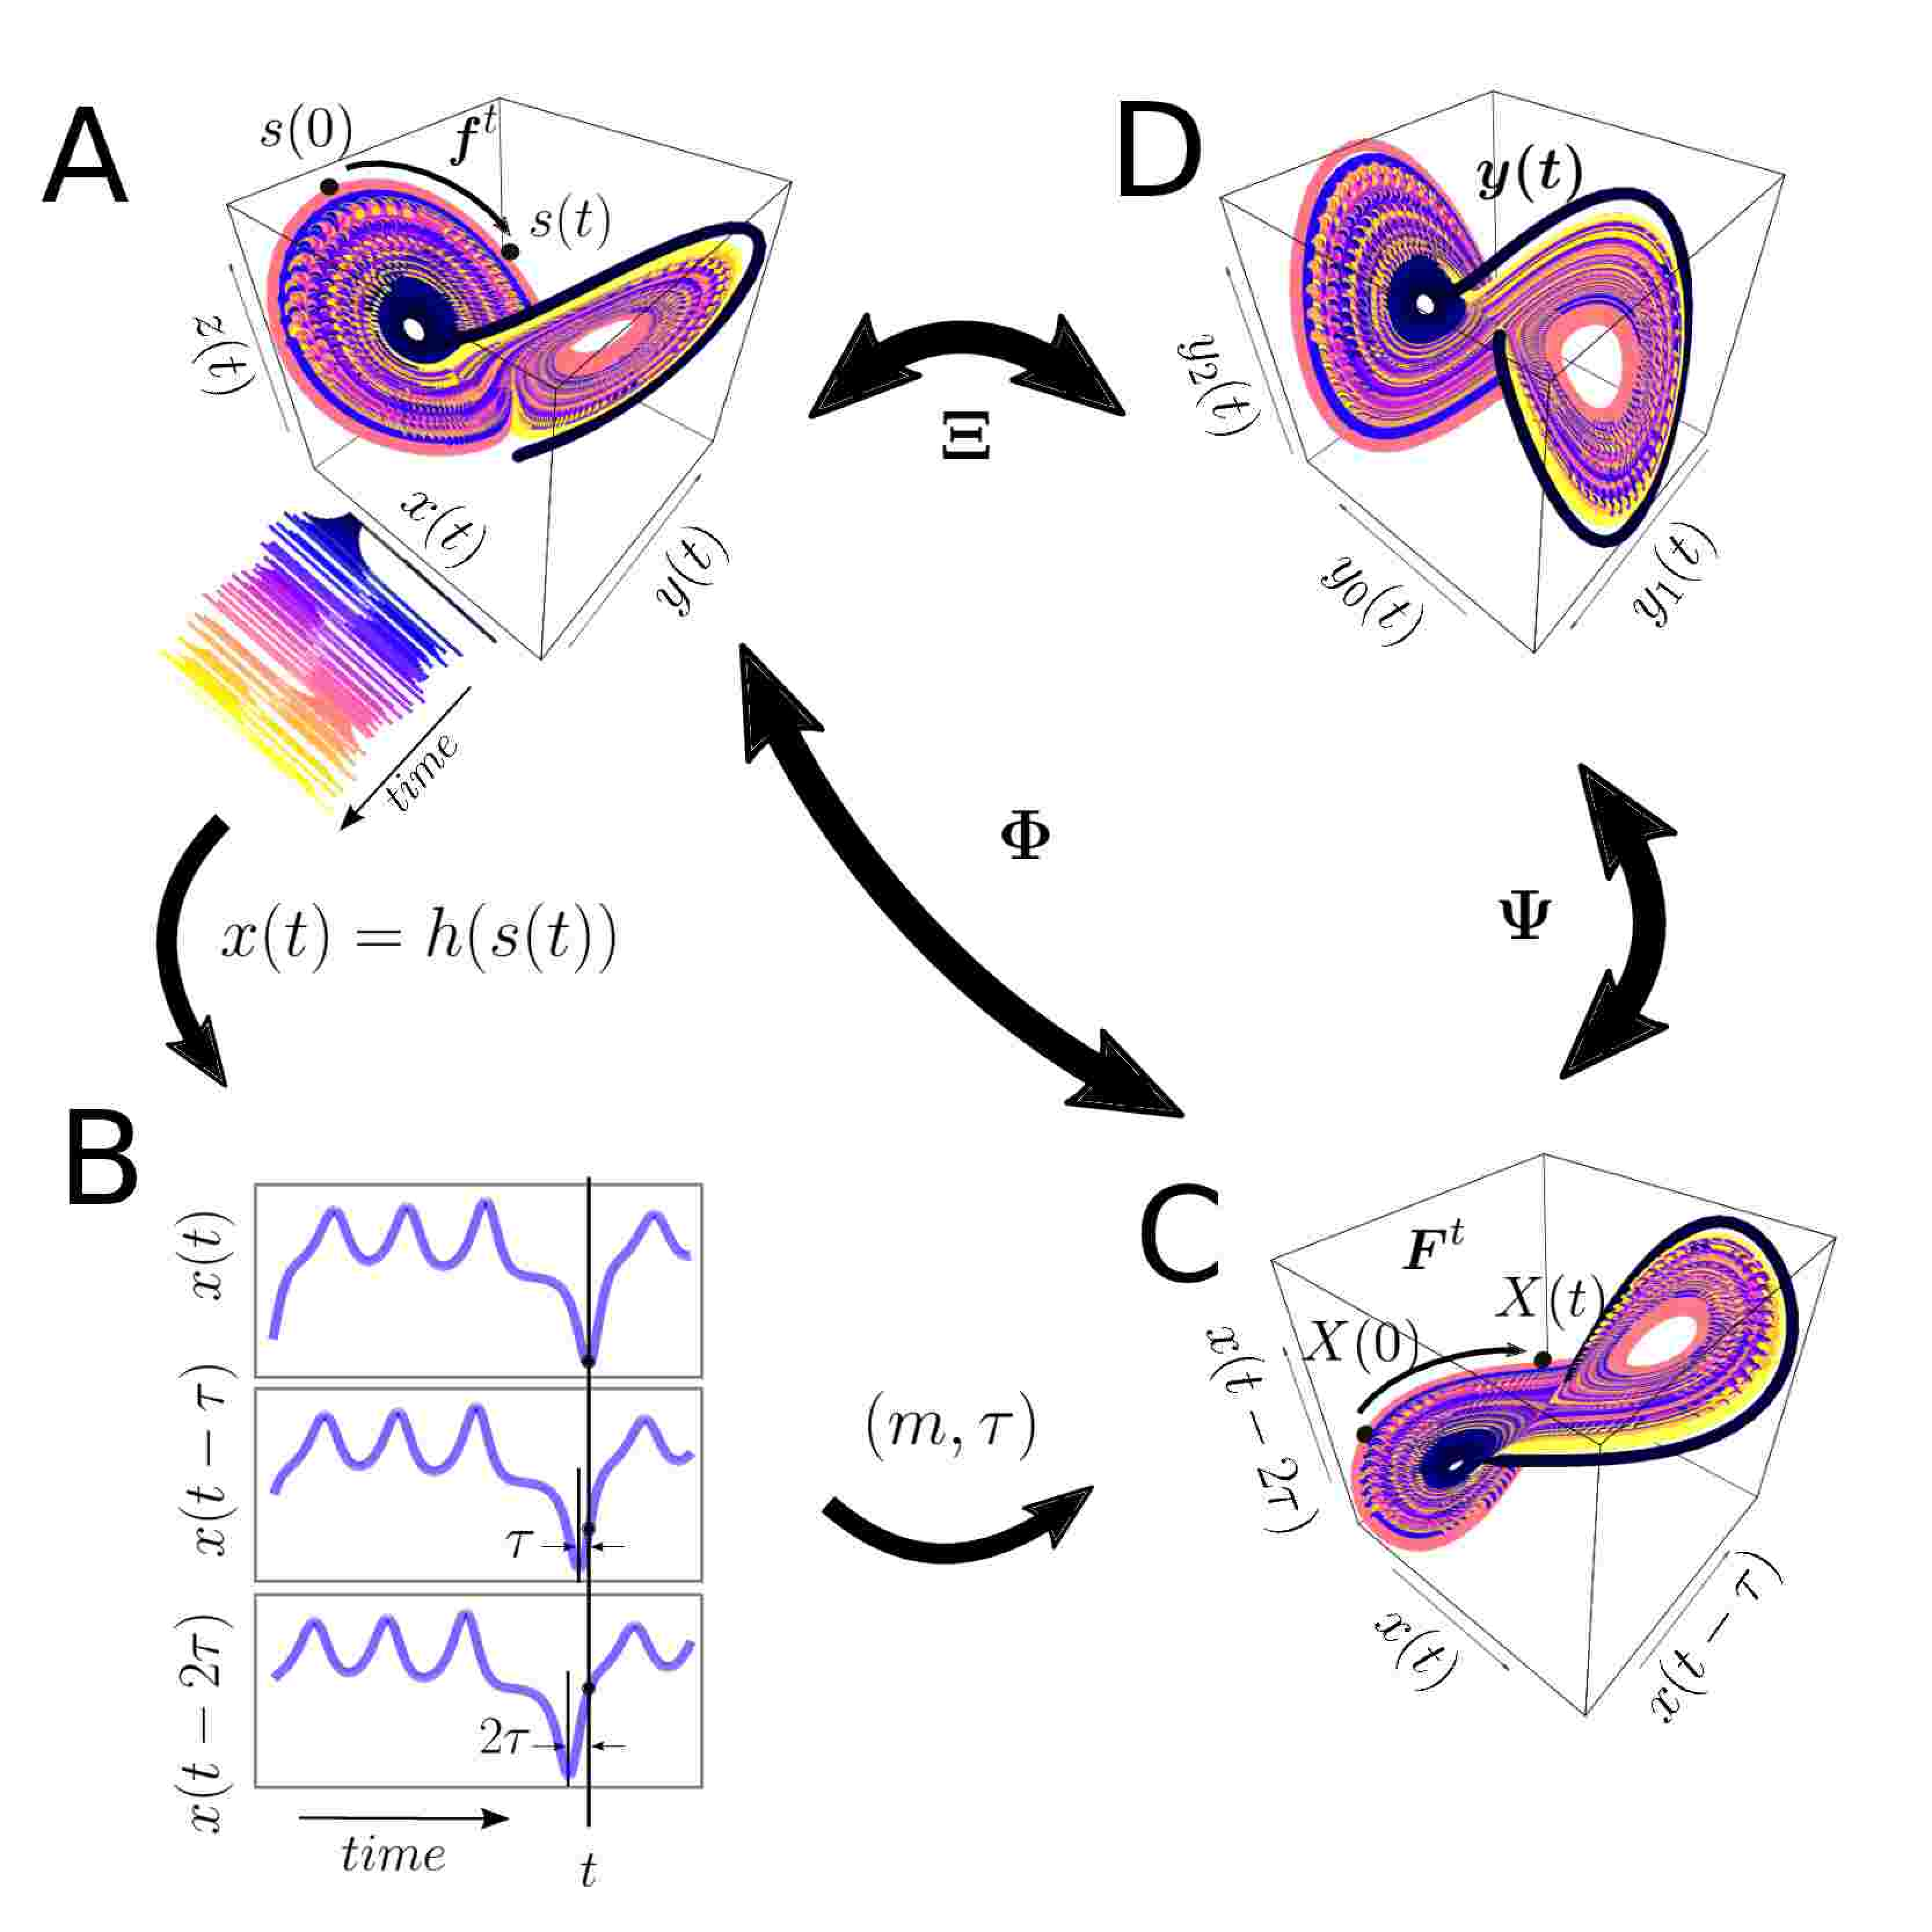
\includegraphics[width=1.0\textwidth]{fig-rss.pdf}
    \caption{
	{\bf State space reconstruction methodology.}
	State space reconstruction is based on $x(t)=h[s(t)]= h[f^t [s(0)]]$
	where $f^t$ is the true dynamical system, $s(t)$ indicates the state,
    	$s$, at time, $t$,  and $h[ ]$ the measurement function. 
    	The time-delay embedding represented as the $\Phi$, maps the original
    	$d-$dimensional state $s(t)$ into the $m-$dimensional uniform 
	time-delay embedding matrix $\boldsymbol{X}(t)$.
    	The transformation map $\Psi$ then maps $\boldsymbol{X}(t)$ into 
	a new state $y(t)$ of dimensions $n < m$.
    	(A) $M-$dimensional manifold representing the state space 
	(e.g. Lorenz system);
    	(B) Delayed copies of $1-$dimensional $x(t)$ from the Lorenz system;
   	(C) $m-$dimensional reconstructed state space with 
    	\texorpdfstring{$m$}{m} and    \texorpdfstring{$\tau$}{T}, and 
    	(D) $y(t)$ is the $n-$dimensional reconstructed state space.
	The total reconstruction map is represented as $\Xi = \Psi \circ \Phi $
	where $\Phi$ is the delay reconstruction map and 
	$\Psi$ is the coordinate transformation map.
	This figure is adapted from 
   	\cite{Quintana-Duque2012, casdagli1991, uzal2011}.
	Code and data to reproduce the figure is available in \cite{srep2020}.
    }
    \label{fig:ssr}
\end{figure}
%%---------------------------------(FIGURE)-------------------------------------



\subsection*{Uniform Time-Delay Embedding (UTDE)}\label{sec:utimedelayembedding}
Frank et al. and Sama et al. refer to the state space reconstruction
as "time-delay embeddings" or "delay coordinates" \cite{frank2010, sama2013}. 
However, we consider the term "uniform time-delay embedding"
as more descriptive and appropriate terminology for our work.
Hence, the uniform time-delay embedding is represented as a matrix of uniform delayed 
copies of the time series $\{ \boldsymbol{x}_n \}_{n=1}^N$ where $N$ is 
the sample length of $\{ \boldsymbol{x}_n \}$ and $n$ is index for the 
samples of $\{ \boldsymbol{x}_n \}$.
$\{ \boldsymbol{x}_n \}_{n=1}^N$ has a sample rate of $T$.
The delayed copies of $\{ \boldsymbol{x}_n \}$ are uniformly separated by $\tau$
and represented as $\{\boldsymbol{ \tilde{x} }_{n- i\tau} \}$
where $i$ goes from $0,1, \dots, (m-1)$.
Generally speaking, $\{\boldsymbol{ \tilde{x} }_{n- i\tau} \}$ contains
information of unobserved state variables and encapsulates the information of
the delayed copies of the available time series in the uniform time-delay 
embedding matrix $\boldsymbol{X}^{m}_{\tau}$, 
$\boldsymbol{X}^{m}_{\tau} \in \mathbb{R}^m$, defined as
%%********************************[EQUATION]************************************
\begin{equation}\label{eq:tde}
\boldsymbol{X}^{m}_{\tau}  =
\begin{pmatrix}
\boldsymbol{ \tilde{x} }_n \\
\boldsymbol{ \tilde{x} }_{n-\tau} \\
\boldsymbol{ \tilde{x} }_{n-2\tau} \\
\vdots \\
\boldsymbol{ \tilde{x} }_{n- (m-1) \tau} \\
\end{pmatrix}^\intercal, 
\end{equation}
%%********************************[EQUATION]************************************
where $m$ is the embedding dimension, $\tau$ is the embedding delay and
$ ^\intercal$ denotes the transpose.
$m$ and $\tau$ are known as embedding parameters.
The matrix dimension of $ \boldsymbol{X}_{\tau}^{m} $ is defined by
$N-(m-1)\tau$ rows and $m$ columns and 
$N-(m-1)\tau$ defines the length of each delayed copy 
of $\{ \boldsymbol{ \tilde{x} }_n \}$ in $\boldsymbol{X}^{m}_{\tau}$.
%For further details and explicit examples of uniform time-delay 
%embedding methodology, we refer the reader to the \nameref{S1_AppendixA}.




\subsection*{Estimation of Embedding Parameters}
The estimation of the embedding parameters ($m$ and $\tau$) 
is a fundamental step for the state space reconstruction with the use
of uniform time-delay embedding method.
With this in mind, we review two of the most common algorithms,
which will be used in our work, to compute the embedding
parameters: the false nearest neighbour (FNN) and the average mutual information (AMI).

%%%%%%%%%%%%%%%%%%%%%%%%%%%%%%%%%%%%%%%%%%%%%%%%%%%%%%%%%%%%%%%%%%%%%%%%%%%%%%%%
%*******************************************************************************
\subsubsection*{False Nearest Neighbours}
To select the minimum embedding dimension $m_0$, Kennel et al. \cite{kennel1992}
used the method of false neighbours which can be understood as follows:
on the one hand, when the embedding dimension is too small to unfold the 
attractor "not all points that lie close each other will be neighbours and 
some points appear as neighbours because of the attractor has been projected 
down into an smaller space", on the other hand, when increasing the embedding 
dimension "points that are near to each other in the sufficient
embedding dimension should remain close as the dimension increase from $m$ 
to $m+1$ \cite{krakovska2015}".
From a mathematical point of view, the state space reconstruction theorem is 
done when the attractor is unfolded with either the minimum embedding 
dimension, $m_0$, or any other embedding dimension value where 
$m \ge m_0$ \cite{kennel1992}. On the contrary, any large value of $m_0$ 
leads to excessive computations \cite{bradley2015}. With this in mind, 
Cao \cite{Cao1997} proposed an algorithm based on the false neighbour method 
where only the time-series and one delay embedding value are necessary 
to select the minimum embedding dimension. Cao's algorithm is based 
on $E(m)$  which is the mean value of all $a(i,m)$, both defined as follows
%%********************************[EQUATION]************************************
\begin{equation}\label{eq:e}
  \begin{aligned}
	E(m) &= \frac{1}{N-m\tau} \sum_{i=1}^{N-m\tau} a(i,m) \\
	 &=
       \frac{1}{N-m\tau} \sum_{i=1}^{N-m\tau}
       \frac{ || \boldsymbol{X}_i(m+1) - \boldsymbol{X}_{n(i,m)}(m+1) || }
            { || \boldsymbol{X}_i(m) - \boldsymbol{X}_{n(i,m)}(m) ||  }
  \end{aligned}
\end{equation}
%%********************************[EQUATION]************************************
where $\boldsymbol{X}_i(m)$ and $\boldsymbol{X}_{n(i,m)}(m)$ are the time-delay
embeddings with $i=1,2,\dots,N-(m-1)\tau$ and $ n(i,m)= 1 \le n(i,m) \le N-m\tau$.
From Eq.~\ref{eq:e}, it can be seen that $E(m)$ is only dependent on $m$ 
and $\tau$ for which $E_1(m)$ is defined as
%%********************************[EQUATION]************************************
\begin{equation}\label{eq:e1}
E_1(m) = \frac{ E(m+1) } { E(m)}.
\end{equation}
%%********************************[EQUATION]************************************
$E_1(m)$ is therefore considered to investigate the variation from $m$ to $m+1$
in order to find the minimum embedding dimension $m_0$ (Eq.~\ref{eq:e1}).
As described in \cite{Cao1997}: "$E_1(m)$ stops changing when $m$ is greater
than some $m_0$, if the time series comes from a multidimensional state space
then $m_0 + 1$ is the minimum dimension".
Additionally, Cao proposed $E_2(m)$ to distinguish deterministic signals from
stochastic signals. $E_2(m)$ is defined as
%%********************************[EQUATION]************************************
\begin{equation}\label{eq:e2}
E_2(m) = \frac{ E^* (m+1) } { E^*(m)},
\end{equation}
%%********************************[EQUATION]************************************
where
%%********************************[EQUATION]************************************
\begin{equation}\label{eq:ee}
E^*(m) = \frac{1}{N-m\tau} \sum_{i=1}^{N-m\tau}
|  \boldsymbol{X}_i(m+1) - \boldsymbol{X}_{n(i,m)}(m+1) |.
\end{equation}
%%********************************[EQUATION]************************************
For instance, when the signal comes from random noise (values that are 
independent from each other), all $E_2(m)$ values are approximately equal 
to 1 (e.g. $E_2(m) \approx 1$). However, for deterministic data $E_2(m)$ is 
not constant for all $m$ (e.g. $E_2(m) \neq 1$).

As an example of the use of $E_1(m)$ and $E_2(m)$ values, we consider two time 
series: the solution for the $x$ variable of the Lorenz system 
(Fig~\ref{fig:caoami}A), and a Gaussian noise time series with zero mean 
and a variance of one (Fig~\ref{fig:caoami}B).
We then compute $E_1(m)$ and $E_2(m)$ values for each time series.
The $E_1(m)$ values for the chaotic time series appear to be constant
after the dimension is equal to six.
The determination of six is given that any value of $m$ can be used as they 
are within the threshold of $1\pm0.05$ (Fig~\ref{fig:caoami}C).
$E_2(m)$ values, for chaotic time series, are different to one 
(Fig~\ref{fig:caoami}E), for which, it can be concluded that for the 
chaotic time series the minimum embedding dimension the time series 
comes from a deterministic signal. With regard to the noise time series,  
$E_1(m)$ values appeared to be constant when $m$ is close to thirteen, 
which is defined by the threshold of $1\pm0.05$ (Fig~\ref{fig:caoami}D).
$E_1(m)$ values then indicate the minimum embedding dimension of the 
noisy time series is thirteen, however all of the $E_2(m)$ values are 
approximately equal to one (Figure~\ref{fig:caoami}F) for which it can be 
concluded that noise time series is a stochastic signal.
It is important to note that for this work not only $E_1(m)$ and $E_2(m)$ are 
computed but also a variation of $\tau$ from 1 to 20 is presented. 
The purpose of such variation for $\tau$ is to show its independence with
regard to $E_1(m)$ and $E_2(m)$ values as $\tau$ is increasing 
(Fig~\ref{fig:caoami}C,D,E and F). 
However, one negative of the Cao's algorithm \cite{Cao1997} is the definition of 
a new threshold where $m$ values appear to be constant in $E_1 (m)$.
In the case of the given examples and reported results, we defined such 
threshold as 0.05. Further investigation is required for the selection of the 
threshold in the $E_1(m)$, as the selection of the threshold in this work is 
base on no particular method but visual inspection.

%%%%%%%%%%%%%%%%%%%%%%%%%%%%%%%%%%%%%%%%%%%%%%%%%%%%%%%%%%%%%%%%%%%%%%%%%%%%%%%%
%*******************************************************************************
\subsubsection*{Average Mutual Information}
When selecting the delay dimension parameter, $\tau$, one can consider the 
following two cases:
(i) when $\tau$ is too small, the elements of time-delay embedding will be along
the bisectrix of the phase space and the reconstruction is generally not 
satisfactory, 
(ii) on the contraty, when $\tau$ is too large the elements of the uniform 
time-delay embedding will become spread and uncorrelated which makes 
recovering the underlying attractor more difficult if not 
impossible \cite{casdagli1991, emrani2014a, garcia2005e71}.
With regard to the algorithms to compute $\tau$, 
Emrani et al. \cite{emrani2014a}, for instance, used the autocorrelation 
function in which the first zero crossing is considered as the minimum delay 
embedding parameter. However, the autocorrelation function is a linear 
statistic over which the Average Mutual Information (AMI) algorithm is 
preferred because the AMI takes into account the nonlinear dynamical 
correlations \cite{afraser1986,krakovska2015}. With this in mind, the AMI 
algorithm is described below to estimate the minimum delay embedding 
parameter, \texorpdfstring{$\tau_0$}{T}.

To compute the AMI, an histogram of $x(n)$ using $n$ bins is calculated
and then a probability distribution of data is computed \cite{kantz2003}.
AMI is therefore denoted by $I(\tau)$ which is the average mutual 
information between the original time series, $x(n)$, and the delayed 
time series, $x(n-\tau)$, delayed by $\tau$ \cite{kabiraj2012}. 
AMI is defined by
%%********************************[EQUATION]************************************
\begin{equation}\label{eq:ami}
I(\tau) = \sum_{i,j}^N p_{ij} log_2 \frac{ p_{ij} }{ p_i p_j }.
\end{equation}
%%********************************[EQUATION]************************************
Probabilities are defined as follows:
$p_i$ is the probability that $x(n)$ has a value inside the $i$-th bin of 
the histogram, $p_j$ is the probability that $x(n+\tau)$ has a value inside 
the $j$-th bin of the histogram and $p_{ij}(\tau)$ the probability 
that $x(n)$ is in bin $i$ and $x(n+\tau)$ is in bin $j$. The AMI is measured 
in bits (base 2, also called shannons) \cite{kantz2003, nonlinearTseries2016}.
For small $\tau$, AMI will be large and it will then decrease more or 
less rapidly. As $\tau$ increase and goes to a large limit, 
$x(n)$ and $x(n+\tau)$ have nothing to do with each other and $p_(ij)$ is 
factorised as $p_ip_j$ for which AMI is close to zero. Then, in order 
to obtain $\tau_0$, "it has to be found the first minimum of $I(\tau)$ 
where $x(n+\tau)$ adds maximal information to the knowledge from $x(n)$, or,
where the redundancy is the least" \cite{kantz2003}.

For example, we compute the AMI for two time series:
A) the $x$ solution of the Lorenz system, and
B) a noise time series using a normal distribution with mean zero and 
standard deviation equal to one. From Fig~\ref{fig:caoami}(G, H), it can then be 
concluded that the amount of knowledge for any noise time series is zero 
for which the first minimum embedding parameter is $\tau_0=1$. 
On the contrary, the first minimum of the AMI for the chaotic time series 
is $\tau_0=17$ which is the value that maximize the independence 
between $x(n)$ and $x(n+\tau)$ in the reconstructed state space 
\cite{bradley2015}.
%%---------------------------------(FIGURE)-------------------------------------
Similarly as Cao's algorithm negatives, AMI's algorithm is not an
exception for negatives, which are worthwhile to mention for further 
investigations.
For instance, (i) is not clear why the choose of the first minimum of the AMI 
is the minimum delay embedding parameter \cite{kantz2003} and 
(ii) the probability distribution of the AMI function is computed
with the use of histograms which depends on a heuristic choice of number of bins
for which AMI depends on partitioning \cite{garcia2005e71}.

%%---------------------------------(FIGURE)-------------------------------------
\begin{figure}[ht]
\centering
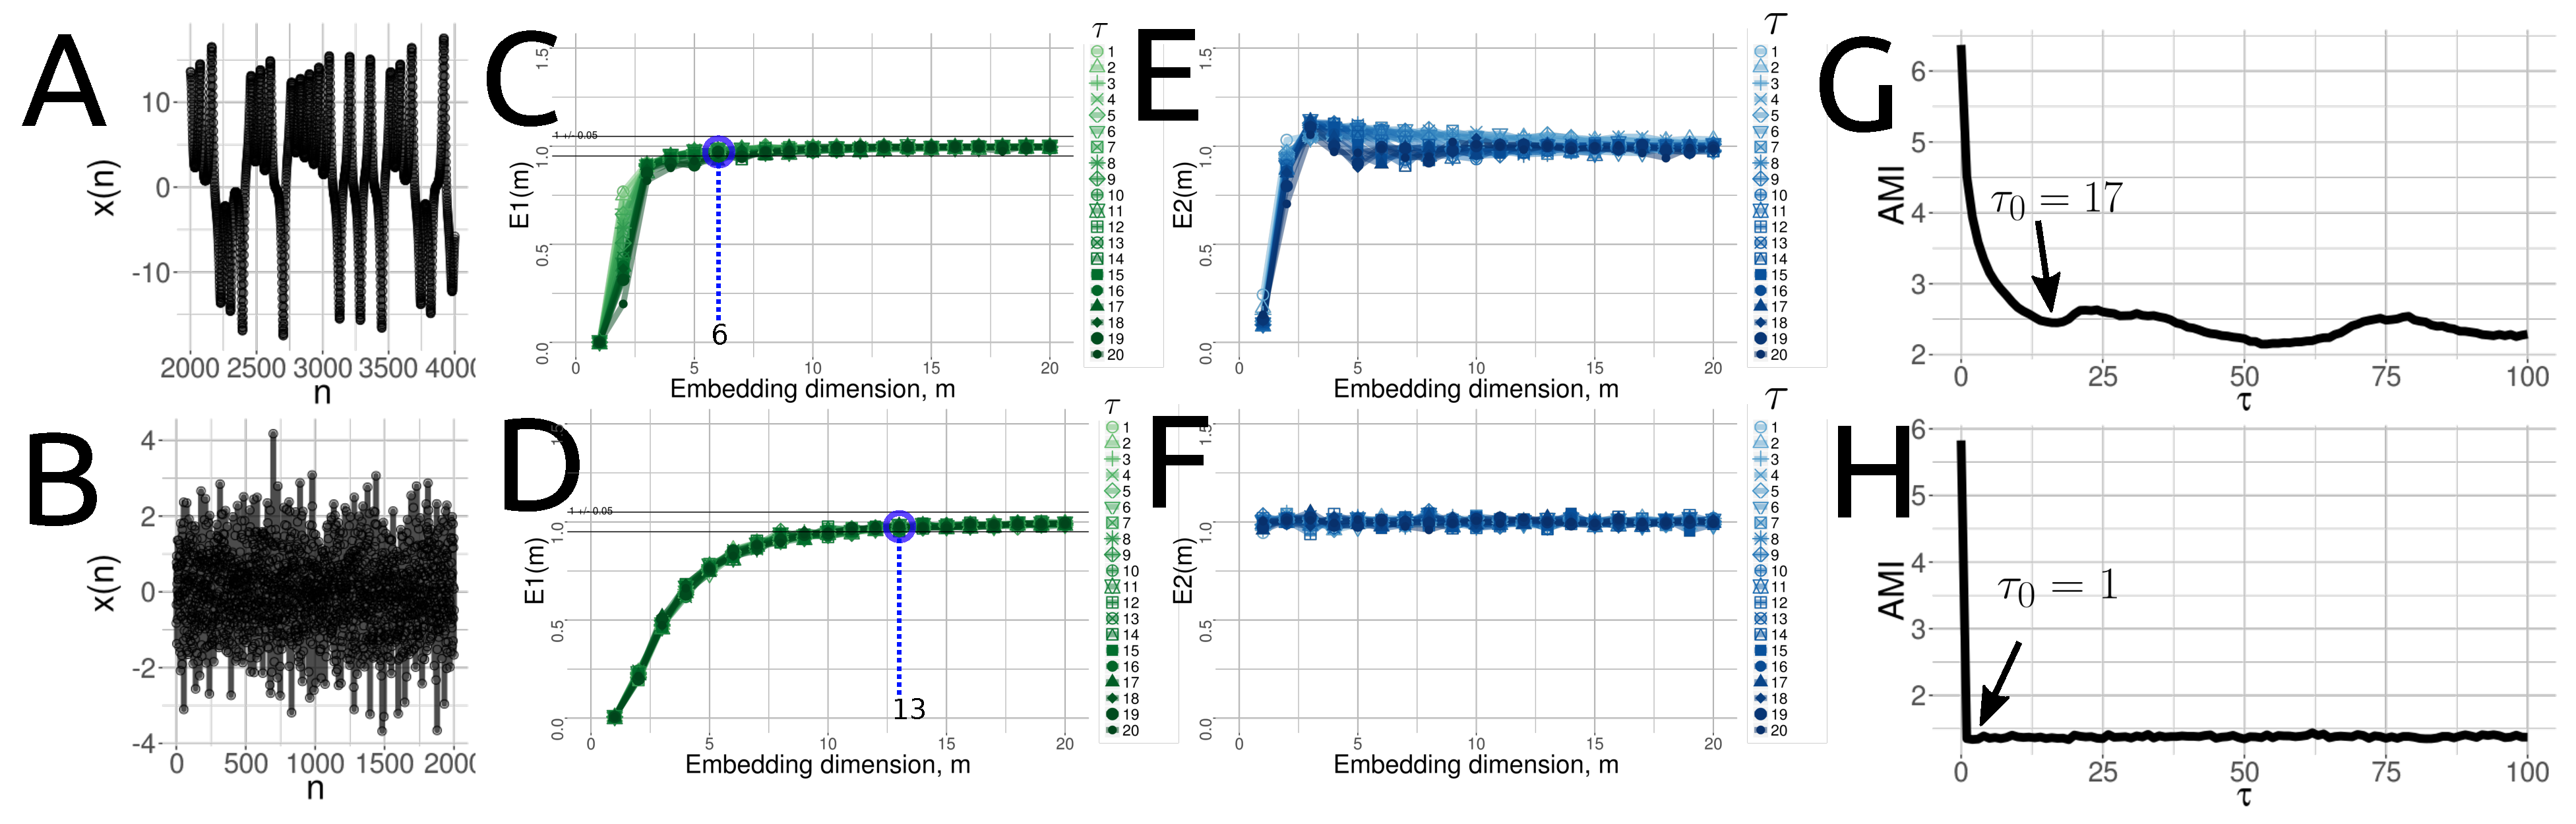
\includegraphics[width=1.0\textwidth]{fig-caoami.pdf}
    \caption{
	{\bf Minimum delay embedding values with AMI's method and minimum dimension embedding values with Cao's method.} 
	(A) chaotic and (B) random time series.
	(C, D) $E_1 (m)$ values and (E, F) $E_2(m)$ values 
	with variations of $\tau$ values from one to twenty
	for chaotic and random time series.
	(G, H) AMI values where its first minimum value in the curve
	is the minimum time delay embedding ($\tau_0$).
	Code and data to reproduce the figure is available in \cite{srep2020}.
        }
    \label{fig:caoami}
\end{figure}
%%---------------------------------(FIGURE)-------------------------------------


%*******************************************************************************
\section*{Recurrence Quantification}\label{sec:recurrence-quantification}
\subsection*{Recurrence Plots}
Originally, Henri Poincar\'e in 1890 introduced the concept of recurrences 
in conservative systems, however such discovery was not put into practice 
until the development of faster computers \cite{marwan2007},
for which Eckmann et al. \cite{eckmann1987} in 1987 introduced a method
where recurrences in the dynamics of a system can be visualised using 
Recurrence Plots. The intention of Eckmann et al. \cite{eckmann1987} was to 
propose a tool, called Recurrence Plot (RP), that provides insights into 
high-dimensional dynamical systems where trajectories are very difficult to 
visualise. Therefore, "RP helps us to investigate the 
$m-$dimensional phase space trajectories through a two-dimensional 
representation of its recurrences" \cite{marwan2015}.
Similarly, Marwan et al. \cite{marwan2015} pointed out that additionally 
to the methodologies of the state space reconstruction and other dynamic 
invariants such as Lyapunov exponent, Kolmogorov-Sinai entropy, 
the recurrences of the trajectories in the phase space can provide 
important clues to characterise natural process that present, for
instance, periodicities (as Milankovitch cycles) or irregular cycles 
(as El Ni\~no Southern Oscillation). 
Such recurrences can not only be presented visually using Recurrence Plots (RP) 
but also be quantified with Recurrence Quantification metrics, which leads 
to applications of these in various areas such as economy, physiology, 
neuroscience, earth science, astrophysics and engineering \cite{marwan2007}.

For the creation of a recurrence plot based on time series 
$\{ \boldsymbol{x}_n \}$, it is first computed the state space 
reconstruction with uniform time-delay embedding 
$X(i)=\{ \boldsymbol{ \tilde{x} }_n, \dots,  
\boldsymbol{ \tilde{x} }_{n -(m-1)\tau} \}$
where $i=1,\dots,N$, $N$ is the number of considered states of $X(i)$ 
and $X(i) \in \mathbb{R}^m$ \cite{eckmann1987}.
The recurrence plot is therefore a two-dimensional $N \times N$ square 
matrix, $\mathbf{R}$, where a black dot is placed at $(i,j)$ 
whenever $X(i)$ is sufficiently close to $X(j)$: 
%%********************************[EQUATION]************************************
\begin{equation}
\mathbf{R}^{m}_{i,j} (\epsilon) = \Theta ( \epsilon_i - || X(i) - X(j) ||
\end{equation}
%%********************************[EQUATION]************************************
where $\quad i,j=1,\dots,N$, $\epsilon$ is a threshold distance, 
$|| \cdotp ||$ a norm, and $\Theta(\cdotp)$ is the Heaviside 
function (i.e. $\Theta(x)=0$, if $x<0$, and $\Theta(x)=1$ otherwise) 
(Fig~\ref{fig:rps}(A,B)) \cite{eckmann1987, marwan2007,marwan2015}.
RP is also characterised with a line of identity (LOI) which is a  
diagonal line due to $ R_{i,j}=1 (i,j=1,\dots,N)$. 


%*******************************************************************************
%*******************************************************************************
%*******************************************************************************
\subsection*{Structures of Recurrence Plots}
Pattern formations in the RPs can be designated either 
as topology for large-scale patterns or texture for small-scale patterns.
In the case of topology, the following pattern formations are commonly presented:
(i) homogeneous where uniform recurrence points are spread in the RP e.g., 
uniformly distributed noise (Fig~\ref{fig:rps}C), 
(ii) periodic and quasi-periodic systems where diagonal lines and 
checkerboard structures represent oscillating systems, e.g., sinusoidal 
signals (Fig~\ref{fig:rps}D), 
(iii) drift where paling or darkening recurrence points away from 
the LOI is caused by drifting systems, 
e.g., logistic map (Fig~\ref{fig:rps}E), and
(iv) disrupted where recurrence points are presented white areas or 
bands that indicate abrupt changes in the dynamics, e.g. Brownian motion 
(Fig~\ref{fig:rps}F) \cite{eckmann1987, marwan2015}.
Texture patterns in RPs can be categorised as:
(i) single or isolated recurrence points that represent rare occurring states, 
and do not persist for any time or fluctuate heavily,
(ii) dots forming diagonal lines where the length of the small-scale parallel 
lines in the diagonal are related to the ratio of determinism or predictability 
in the dynamics of the system, and
(iii) dots forming vertical and horizontal lines where the length of the 
lines represent a time length where a state does not change or change very 
slowly and these patterns formation represent discontinuities in the signal, 
and (iv) dots clustering to inscribe rectangular regions which are related 
to laminar states or singularities \cite{marwan2015}.

Although, each of the previous pattern descriptions of the structures in the 
RP offer an idea of the characteristics of dynamical systems, 
these might be misinterpreted and conclusions might tend to be subjective 
as these require the interpretation of a particular researcher(s).
Because of that, recurrence quantification analyis (RQA) offer objective 
methodologies to quantify such visual characteristics of previous 
recurrent pattern structures in the RP \cite{zbilut1992}.

%---------------------------------(FIGURE)-------------------------------------
\begin{figure}[ht]
\centering
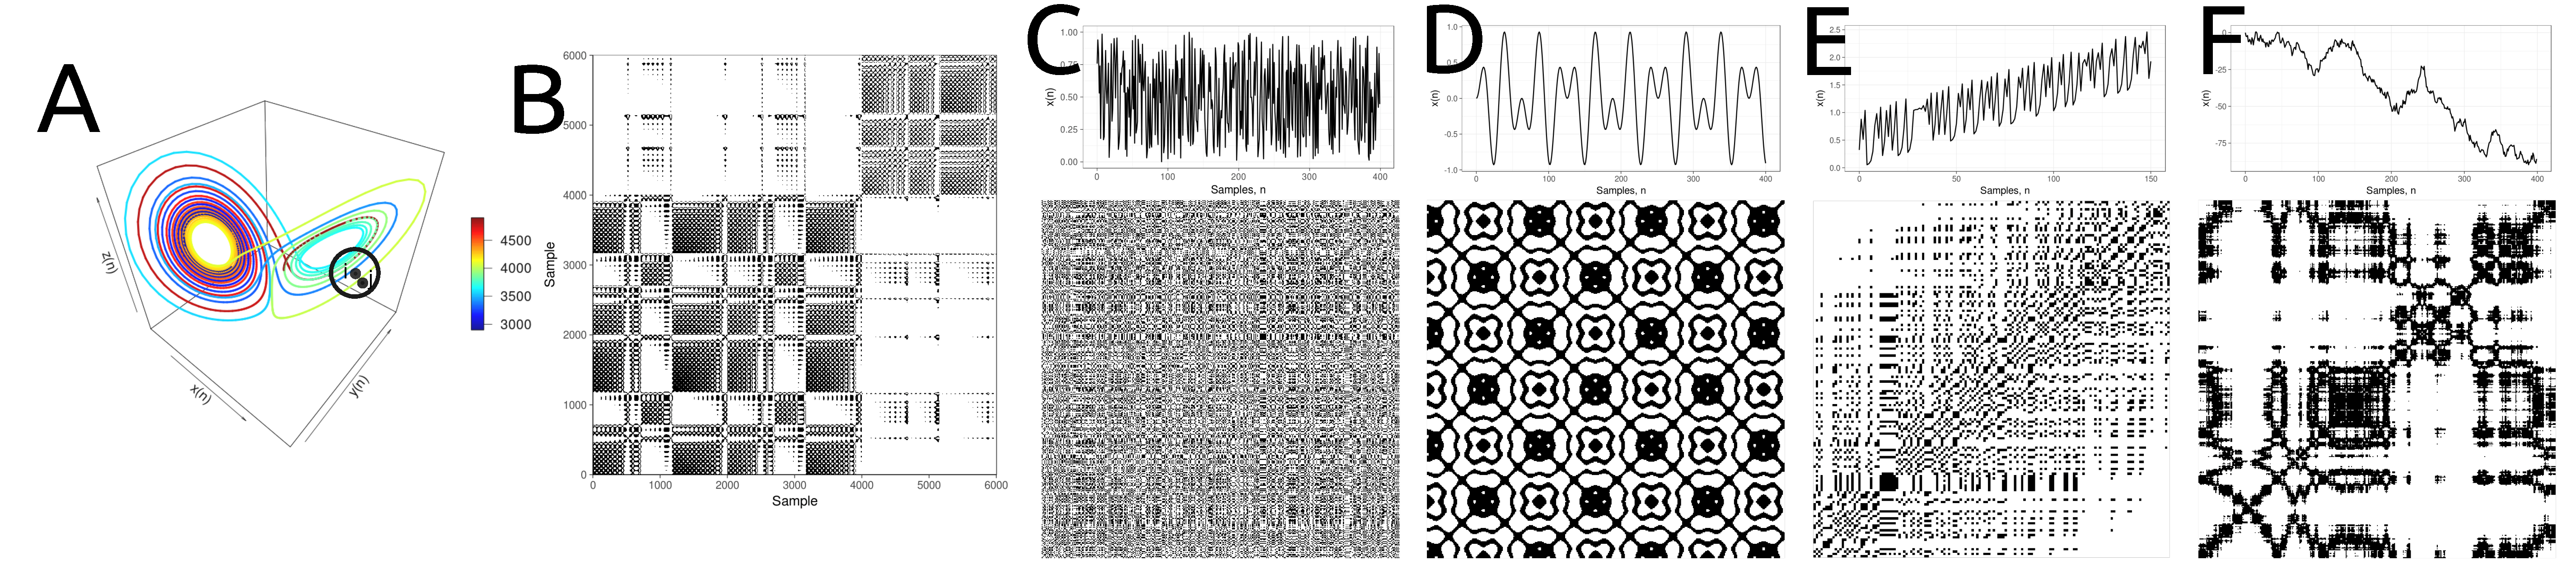
\includegraphics[width=1.0\textwidth]{fig-rps.pdf}
    \caption{
	{\bf Recurrence Plots and its patterns.} 
	(A) State space of the Lorenz system with controlling parameters 
	($\rho=28, \sigma=10, \beta=8/3$) where the point, $j$, in trajectory $X()$ which falls into the neighborhood 
	(black circle) of a given point at $i$ is a recurrent point and is 
	represented as a black dot in the recurrence plot at location 
	$(i, j)$ or white otherwise.
	(B) Recurrence plot using the 
	three components of the Lorenz system and the RP with no embeddings 
	and threshold $\epsilon=5$.
	Time-series with its respective recurrence plot for:
	(C) uniformly distributed noise,
	(D) super-positionet harmonic oscillation 
	($sin( \frac{1}{5}*t) * sin( \frac{5}{100}*t) $),
	(E) drift logistic map ($x_{i+1} = 4 x_i (1- x_i) $) corrupted 
	with a linearly increase term ($0.01*i$), and
	(F) disrupted brownian motion  ($x_{i+1} = x_i + 2*rnorm(1) $).
	This figure is adapted from \cite{marwan2015}.
	Code and data to reproduce the figure is available in \cite{srep2020}.
	}
    \label{fig:rps}
\end{figure}
%%---------------------------------(FIGURE)-------------------------------------



%*******************************************************************************
\subsection*{Recurrence Quantifications Analysis (RQA)}
Originally, Zbilut et al. \cite{zbilut1992} proposed metrics to investigate 
the density of recurrence points in RPs, then histograms of lengths for 
diagonal lines in RPs were studied by \cite{trulla1996} which were the 
introduction to the term recurrence quantification analysis (RQA) 
\cite{marwan2008}. RQA has been applied in many fields such as life science, 
engineering, physics, and others \cite{marwan2008}. Particularly in human 
movement to investigate noise and complexity of postural control 
\cite{rhea2011}, postural control \cite{apthorp2014} or interpersonal 
coordination \cite{duran2017}. The success of RQA is not only due to its 
simple algorithmic implementation but also to its capacity to detect tiny 
modulations in frequency or phase which are not detectable using standard 
methods e.g. spectral or wavelet analysis \cite{marwan2011}, and that 
RQA's metrics are quantitatively and qualitatively independe]nt of embedding 
dimension which is verified experimentally by \cite{iwanski1998}.
RQA metrics comprehend percentage of recurrence, percentage of determinism, 
ratio, Shannon entropy of the frequency distributions of the line lengths,
maximal line length and divergence, trend and laminariy 
\cite{marwan2007, marwan2015}. For this work, we considered only four 
RQA metrics, due to its consistency with our preliminary experiments, 
which are described below. Such metrics are computed the nonlinearTseries 
R package \cite{nonlinearTseries2016}.

\subsubsection*{REC values}
The percentage of recurrence (REC) is defined as
%%********************************[EQUATION]************************************
\begin{equation}
REC(\epsilon,N) = 
		\frac{1}{N^2 - N} \sum^{N}_{i \neq j = 1} 
		\mathbf{R}^{m}_{i,j}(\epsilon),
\end{equation}
%%********************************[EQUATION]************************************
which enumerates the black dots in the RP excluding the line of identity.
REC is a measure of the relative density of recurrence points in the sparse 
matrix \cite{marwan2015}.
%REC is computed as follow with the nonlinearTseries package 
% \cite{nonlinearTseries} 
%  hist = getHistograms(neighs, ntakens, lmin, vmin)
%  # calculate the number of recurrence points from the recurrence rate. The
%  # recurrence rate counts the number of points at every distance in a concrete
%  # side of the main diagonal.
%  # Thus, sum all points for all distances, multiply by 2 (count both sides) and
%  # add the maindiagonal
%  numberRecurrencePoints = sum(hist$recurrenceHist) + ntakens
%  # calculate the recurrence rate dividing the number of recurrent points at a
%  # given distance by all points that could be at that distance
%  recurrence_rate_vector = 
%  hist$recurrenceHist[1:(ntakens - 1)] / ((ntakens - 1):1)
%  # percentage of recurrent points
%  REC = (numberRecurrencePoints) / ntakens ^ 2

\subsubsection*{DET values} 
The percent determinism (DET) is defined as the fraction of recurrence points
that form diagonal lines and it is determined by
%%********************************[EQUATION]************************************
\begin{equation}
DET=
	\frac{\sum^{N}_{l=d_{min}} l H_D{l} }
	     {\sum^{N}_{i,j=1} \mathbf{R}_{i,j}(\epsilon) },
\end{equation}
%%********************************[EQUATION]************************************
where 
%%********************************[EQUATION]************************************
\begin{equation}
H_D(l) = 
	\sum^{N}_{i,j=1} 
	(1- \mathbf{R}_{i-1,j-1}(\epsilon) ) 
	(1- \mathbf{R}_{i+l,j+l}(\epsilon) ) 
	\prod^{l-1}_{k=0}  \mathbf{R}_{i+k,j+k}(\epsilon)
\end{equation}
%%********************************[EQUATION]************************************
is the histogram of the lengths of the diagonal structures in the RP.
DET can be interpreted as the predictability of the system for periodic signals 
which, in essence, have longer diagonal lines than the short diagonals lines
for chaotic signals or absent diagonal lines for stochastic signals 
\cite{marwan2007, marwan2015}. Similarly, DET is considered as a measurement for 
the organisation of points in RPs  \cite{iwanski1998}. 
%percent determinism (DET) is computed as follow with the nonlinearTseries 
%package \cite{nonlinearTseries}  
% calculateDiagonalParameters = function(ntakens, numberRecurrencePoints,
%                                       lmin = 2, lDiagonalHistogram,
%                                       recurrence_rate_vector, maxDistanceMD) {
%  #begin parameter computations
%  num = sum((lmin:ntakens) * lDiagonalHistogram[lmin:ntakens])
%  DET = num / numberRecurrencePoints


\subsubsection*{RATIO values}
RATIO is defined as the ratio between DET and REC and it is calculated from 
the frequency distributions of the lengths of the diagonal lines.
RATIO is useful to discover dynamic transitions \cite{marwan2015}.
%  diagP = calculateDiagonalParameters(
%    ntakens, numberRecurrencePoints, lmin, hist$diagonalHist,
%    recurrence_rate_vector, maxDistanceMD
%  )
% calculateDiagonalParameters = function(ntakens, numberRecurrencePoints,
%                                       lmin = 2, lDiagonalHistogram,
%                                       recurrence_rate_vector, maxDistanceMD) {
%  #begin parameter computations
%  num = sum((lmin:ntakens) * lDiagonalHistogram[lmin:ntakens])
%  DET = num / numberRecurrencePoints
% 
%
%    RATIO = diagP$DET / REC
%

\subsubsection*{ENT values}
ENT is the Shannon entropy of the frequency distribution of the diagonal 
line lengths and it is defined as
%%********************************[EQUATION]************************************
\begin{equation}
ENT= - \sum^{N}_{l=d_{min}} p(l) ln p(l) \quad with 
	\quad p(l)=\frac{ H_D(l) }{ \sum^{N}_{ l=d_{min} } H_D(l) }.
\end{equation}
%%********************************[EQUATION]************************************
ENT reflects the complexity of the deterministic structure in the system.
For instance, for uncorrelated noise or oscillations, 
the value of ENT is rather small and indicates low complexity of the system,
therefore "the higher the ENT is the more complex the dynamics are" 
\cite{marwan2007, marwan2015}.
%#'  \item \emph{ENTR}: Shannon entropy of the diagonal line lengths distribution
%
%calculateDiagonalParameters = function(ntakens, numberRecurrencePoints,
%                                       lmin = 2, lDiagonalHistogram,
%                                       recurrence_rate_vector, maxDistanceMD) {
%
%  pl = lDiagonalHistogram / sum(lDiagonalHistogram)
%  diff_0 = which(pl > 0)
%  ENTR = -sum(pl[diff_0] * log(pl[diff_0]))

 
\subsection*{Sensitivity and robustness of RPs and RQA.}
RP and RQA are a very young field in nonlinear dynamics and many questions 
are still open, for instance, different parameters for window length size 
of the time series, embedding parameters or recurrence threshold can 
generate different results in RQA's metrics \cite{marwan2011, eckmann1987}.

The selection of recurrence threshold, $\epsilon$, can depend on the system 
that is analysed. For instance, when studying dynamical invariants $\epsilon$ 
require to be very small, for trajectory reconstruction $\epsilon$ requires 
to have a large thresholds or when studying dynamical transition 
there is little importance about the selection of the threshold 
\cite{marwan2011}. Other criteria for the selection of $\epsilon$ is that 
the recurrence threshold  should be five times larger 
than the standard deviation of the observational noise
or the use of diagonal structures within the RP is suggested in order
to find the optimal recurrence threshold for (quasi-)periodic process 
\cite{marwan2011}.
Similarly, Iwanski et al. \cite{iwanski1998} highlighted the importance 
of choosing the right embedding parameters to perform RQA for which 
many experiments have to be performed using different parameters in order 
to have a better intuition of the nature of the time series and how 
this is represented by using RQA.

With that in mind, this work explores the sensitivity and robustness 
of the window size of time series, embedding parameters for RSS with UTDE 
and recurrence threshold for RP and RQA in order to gain a better insight 
into the underlying time series collected from inertial sensors in the 
context of human-humanoid imitation activities.
%Such changes of recurrence threshold values 
%can modify the patterns in RPs and therefore the values of RQA metrics.
%We therefore computed 3D surfaces to explore the sensibility and robustness of 
%embedding parameters and recurrence threshold in RQA  metrics. Following the 
%same methodology of computing 3D surfaces, we also considered variation of 
%window length size to present RQA metrics dependencies with embedding 
%parameters, recurrence thresholds and window length size.


%Choosing an appropriate recurrence threshold is crucial so as to get 
%meaningful representations in RP and RQA, however, 

%Iwansky et al. \cite{iwanski1998} stated that patterns in Recurrence Plots and 
%metrics for RQA are independent of embedding dimension parameters, 
%however, that is not the case when using 
%different recurrence thresholds. 


%Zbilut et al. \cite{zbilut1992} established RQA metrics with the aim of 
%determining embedding parameters, their method consisted on creating 3D 
%surfaces with RQA metrics with an increase of embedding parameters 
%($m$ and $\tau$), then Zbilut et al. \cite{zbilut1992} explored 
%fluctuations and gradual changes in the 3D surfaces that provide information 
%about the embeddings. Much recently, Marwan et al. \cite{marwan2015} 
%created 3D surfaces for visual selection of not only embedding parameters 
%but also recurrence thresholds. Following same methodologies, we explored 
%the stability and robustness of RQA metrics (REC, DET, RATIO and ENTR)
%using 3D surfaces by an unitary increase of the pair embedding 
%parameters ($0 \ge m \le 10$, $0 \ge \tau \le 10$) and a decimal increase 
%of 0.1 for recurrence thresholds ($ 0.2 \ge \epsilon \le 3 $) 
%(Fig.~\ref{fig:topo_rqas}).



%*******************************************************************************
%*******************************************************************************
%*******************************************************************************
\section*{Experiment} \label{sec:experiment}
We conducted an experiment in the context of human-humanoid imitation (HHI) 
activities where participants were asked to imitate simple horizontal and 
vertical arm movements performed by NAO, a humanoid robot \cite{gouaillier2009}.
Such simple movements were repeated ten times for the participant 
who copied NAO's arm movements in a face-to-face imitation activity.
Also, wearable inertial measurement unit (IMU) sensors were attached 
to the right hand of the participant and to the left hand of the robot 
(Figure~\ref{fig:hri} A,C). Data were then collected with four NeMEMSi 
IMU sensors with sampling rate of 50Hz provinding tri-axial data of the 
accelerometer, gyroscope and magnetometer sensors and quaternions 
\cite{Comotti2014}.
%%---------------------------------(FIGURE)-------------------------------------
\begin{figure}[ht]
  \centering
\includegraphics[width=1.0\textwidth]{fig-hri}
    \caption{
	{\bf Human-humanoid imitation activities.} 
    		Face-to-face human-humanoid imitation (HHI) activities for 
		(A) HHI of horizontal arm movement, 
		(B) Humanoid horizontal arm movement,
		(C) HHI of vertical arm movement, and 
		(D) Humanoid vertical arm movement.
        }
    \label{fig:hri}
\end{figure}
%%---------------------------------(FIGURE)------------------------------------

\subsection*{Participants}
Twenty-three participants,
from now on defined as $pN$ where $N$ is the number of participant, were 
invited to do the experiment. However, data for three participants were 
not used because the instructions for $p01$, who was the only left-handed,
were mistakenly given in a way that movements were performed different
from what had been planned, and for participants $p13$ and $p16$ 
data were corrupted because of problems with Bluetooth communications with sensors. 
With that in mind, data for twenty participants were analysed in this work.
Of the twenty participants, all of them are right-handed healthy participants 
of whom four are females and sixteen are males with a mean and standard 
deviation (SD) age of mean=19.8 (SD=1.39). 

\subsection*{Ethics}
All participants provided informed consent forms prior to participation 
in the experiment. Hence, the experiments were conducted in November 2016 and 
participants confirmed reading and understanding the participant information sheet of the 
experiments and were able to withdraw from the experiment at any time without giving
any reason. The design of the experiments adhered to the University of Birmingham
regulations, data were anonymised and videos were stored only on a 
personal computer in accordance with the Data Protection Act 1998. 
%Refer to Appendix D for further information about the ethics, 
%online participation information sheets and experiment check list.


\subsection*{Human-humanoid imitation activities}
For human-humanoid imitation (HHI) activities four neMEMSi sensors were used,
two of which were attached to the right hand of the participant and the 
other two to the left hand of the humanoid robot.
Then, each participant was asked to imitate repetitions of simple horizontal
and vertical arm movements performed by the humanoid robot in the following 
conditions:
(i) ten repetitions of horizontal arm movement at normal (HN) 
	and faster (HF) speed (Figure~\ref{fig:hri} A), and
(ii) ten repetitions of vertical arm movement at normal (VN) 
	and faster (VF) speed (Figure~\ref{fig:hri} C).
The normal and faster speed of arm movements is defined by the duration 
in number of samples of one repetition of NAO's arm movements. 
We select NAO's arm movements duration to distinguish between normal and 
faster arm movements as NAO's movements have less variation 
for such repetitive movements. 
The duration for one repetition of the horizontal 
arm movement at normal speed, HN, is 5 seconds considering 
that each repetition last around 250 samples.
For horizontal arm movement at faster speed, HF, each repetition were performed 
in 2 seconds which correspond to 90 samples of data.
The vertical arm movement at normal speed, VN, were performed  in 6 seconds 
which is around 300 samples of data. For vertical arm movement at 
faster speed, VF, each repetition lasts about 2.4 seconds which correspond 
to 120 samples of data.
To visualise the distinction between normal and faster speed for horizontal 
and vertical arm movements, Fig~\ref{fig:sts} shows smoothed time series 
for axes Z and Y of the gyroscope sensors with four window lengths: 
2-sec (100-samples), 5-sec (250-samples), 10-sec (500-samples) 
and 15-sec (750-samples).
%%---------------------------------(FIGURE)-------------------------------------
\begin{figure}[ht] 
\centering
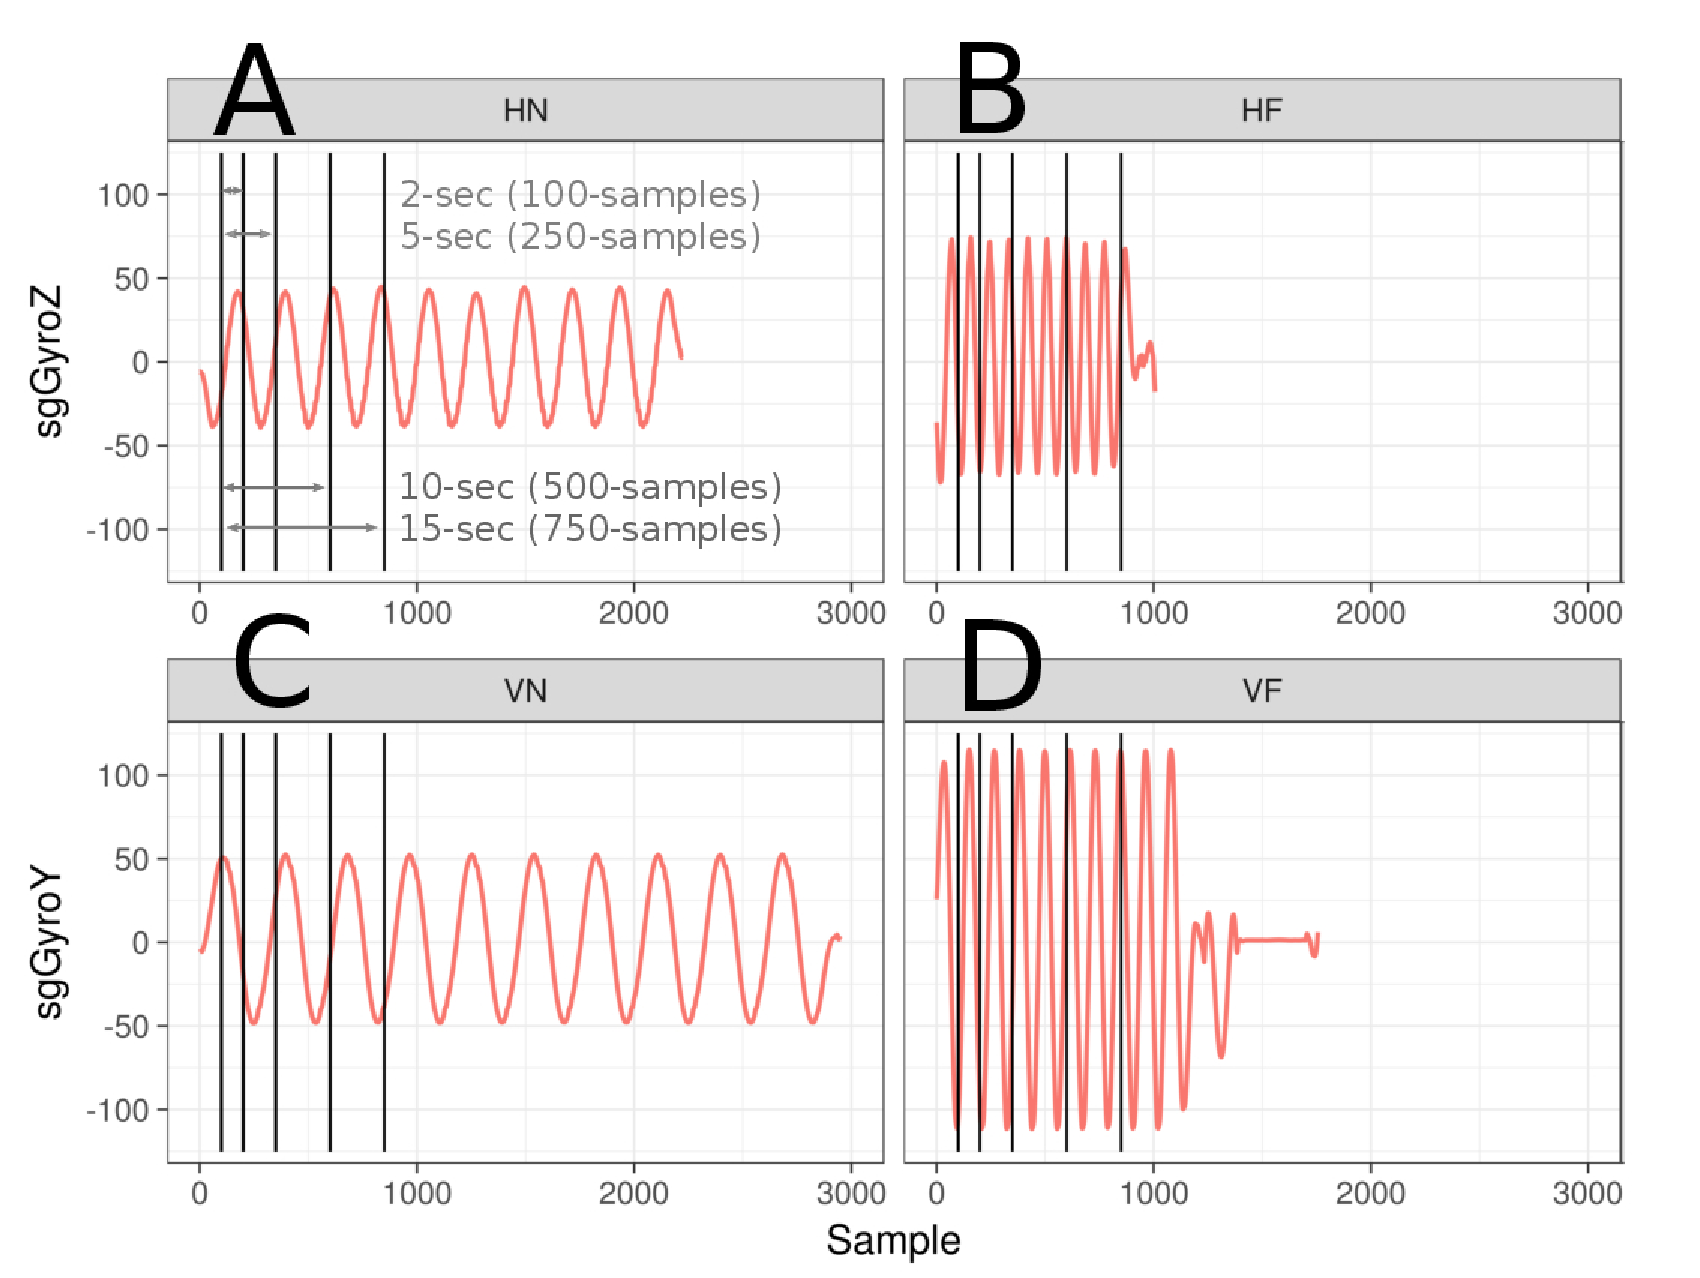
\includegraphics[width=1.0\textwidth]{fig-sts.pdf}
    \caption{
	{\bf Time series duration of horizontal and vertical arm movements.} 
    		Time series of smoothed data from gyroscope sensor 
		for different speed arm movements performed by NAO: 
		(A) Horizontal Normal arm movement (HN), 
		(B) Horizontal Faster arm movement (HF),
		(C) Vertical Normal arm movement (VN) and 
		(D) Vertical Faster arm movement (VF).
		Additionally, 
		(A) shows window sizes for 2-seconds (100 samples), 
		5-seconds (250 samples), 10-seconds (500 samples) 
		and 15-seconds (750 samples)
		which are also presented in (B), (C) and (D).
		Code and data to reproduce the figure is available in \cite{srep2020}.
        }
	\label{fig:sts}
\end{figure}
%%---------------------------------(FIGURE)------------------------------------

\subsection*{Data collection from inertial measurement units} 
\label{sec:experiment:subsec:imu}
To give insight to the research questions, 
we considered various conditions of time series collected for this work: 
\begin{itemize}
\item Three levels of smoothness for normalised data 
	(e.g., sg0zmuv, sg1zmuv and sg2zmuv) where sg 
	stands for Savitzky-Golay filter with two different filter lengths (29 and 159) 
	and the same polynomial degree of 5 using the function \texttt{sgolay(p,n,m)} \cite{Rsignal}
	and zmuv is zero mean unit variance.
\item four arm movement activities with two velocities: 
	horizontal normal (HN), horizontal faster (HF), 
	vertical normal (VN), and vertical faster (VF), and
\item four window lengths: 2-sec (100 samples), 5-sec (250 samples), 
	10-sec (500 samples) and 15-sec (750 samples).
\end{itemize}
%After the data collection, raw time series were windowed, normalised and smoothed. 
Due to space limitations and to have simple visualisation, 
we only present 10-sec (500 samples) window length time series for 
three participants (p01, p01 and p03) performing horizontal 
arm movements (axis GyroZ) and vertical arm movements (axis GyroY) (Figs \ref{fig:ts}).
%%---------------------------------(FIGURE)-------------------------------------
\begin{figure}[ht]
\centering
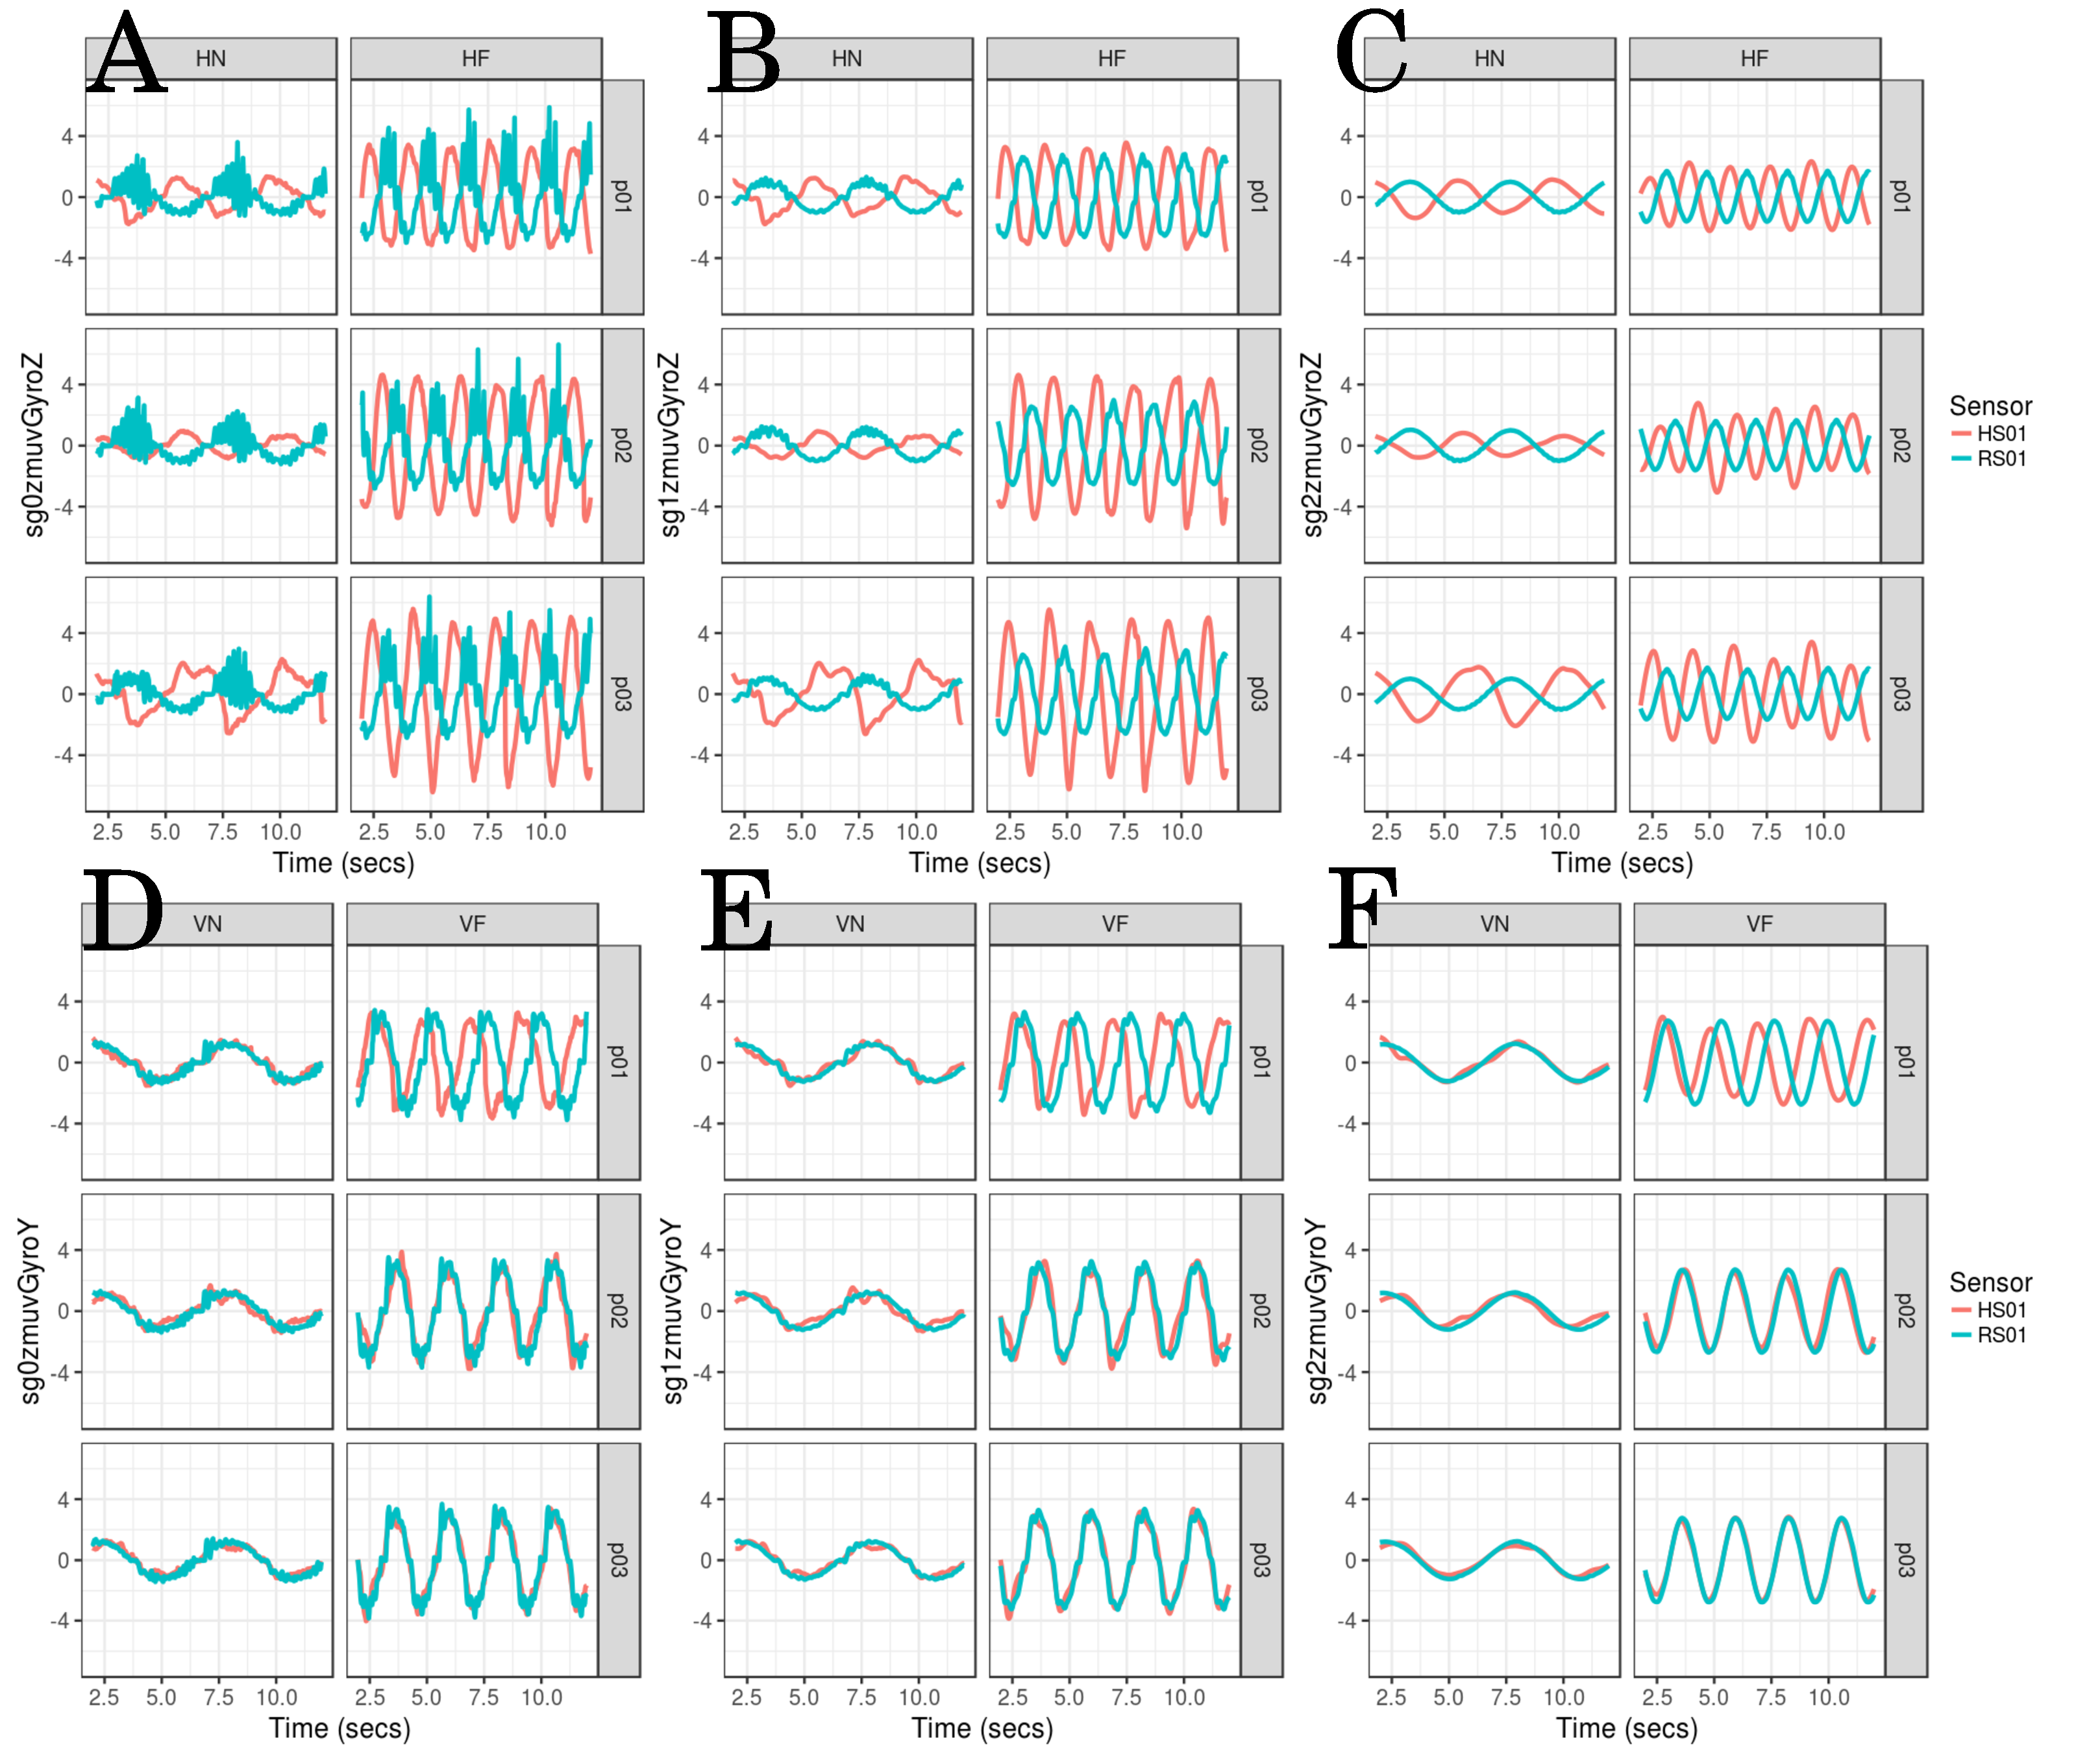
\includegraphics[width=1.0\textwidth]{fig-fig1.pdf}
    	\caption{ 
	{\bf Time series for horizontal and vertical arm movements.}
		(A/D) raw-normalised (sg0zmuv), 
		(B/E) normalised-smoothed 1 (sg1zmuv) and
		(C/F) normalised-smoothed 2 (sg2zmuv).
		Time series are only for three participants 
		($p01$, $p02$, and $p03$) 
		for horizontal and vertical arm movements in normal 
		and faster velocity (HN, HF, VN, VF) 
		with the normalised GyroZ or GyroY axis 
		and with one sensor attached to the participant (HS01) 
		and other sensor attached to the robot (RS01).	
	Code and data to reproduce the figure is available in \cite{srep2020}.
        }
    \label{fig:ts}
\end{figure}
%%---------------------------------(FIGURE)------------------------------------




\subsubsection*{Raw data}
%Considering the work of \cite{shoaib2016} which provided evidence of an 
%improvement in recognition activities when combining data from 
%accelerometer and gyroscope. 
We focus our analysis from data of the 
accelerometer and gyroscope of the NeMEMsi sensors \cite{Comotti2014} and 
leave the data of the magnetometer and quaternions for further investigation 
because of their possible variations with regard to magnetic disturbances \cite{shoaib2016}.
Data from the accelerometer is defined by triaxial time series 
$A_x(n)$, $A_y(n)$, $A_z(n)$ which forms the matrix $\boldsymbol{A}$ 
(Eq.~\ref{eq:AG}), and the same for data from the gyroscope 
which is defined by triaxial time-series of $G_x(n)$, $G_y(n)$, $G_z(n)$ 
representing the matrix $\boldsymbol{G}$ (Eq.~\ref{eq:AG}).
Both triaxial time series of each sensor, $a$ and $g$, are denoted with 
its respective axes subscripts $x,y,z$, where $n$ is the sample index 
and $N$ is the same maximum length of all axes for the time series.
%Matrices  $\boldsymbol{A}$ and $\boldsymbol{G}$ are represented as follows
%%---------------------------------(EQUATION)----------------------------------
\begin{equation}\label{eq:AG}
\boldsymbol{A} =
\begin{pmatrix}
  A_x(n) \\
  A_y(n) \\
  A_z(n)
\end{pmatrix}
=
\begin{pmatrix}
 a_x(1),a_x(2),\dots,a_x(N) \\
 a_y(1),a_y(2),\dots,a_y(N) \\
 a_z(1),a_z(2),\dots,a_z(N) 
\end{pmatrix},
%\end{equation}
%%---------------------------------(EQUATION)-----------------------------------
%and 
%%---------------------------------(EQUATION)-----------------------------------
%\begin{equation}\label{eq:G}
\boldsymbol{G} =
\begin{pmatrix}
 G_x(n) \\
 G_y(n) \\
 G_z(n)
\end{pmatrix}
=
\begin{pmatrix}
 g_x(1),g_x(2),\dots,g_x(N) \\
 g_y(1),g_y(2),\dots,g_y(N) \\
 g_z(1),g_z(2),\dots,g_z(N) 
\end{pmatrix}.
\end{equation}
%%---------------------------------(EQUATION)-----------------------------------


\subsubsection*{Postprocessing data}
After the collection of raw data from four NeMEMsi sensors,
time synchronisation alignment and interpolation were performed 
in order to create time series with the same length and synchronised time.
We refer the reader to \cite{Comotti2014} for further
details about the time synchronisation process.

\subsubsection*{Normalising data}
Data is normalised to be zero mean and unit variance.
The sample mean and sample standard deviation using $x(n)$ is given by
%%---------------------------------(EQUATION)----------------------------------
\begin{equation}\label{eq:ms}
\mu_{x(n)}= \frac{1}{N} ( \sum_{i=1}^N x(i) ), \quad 
	\sigma_{x(n)} =  \sqrt{ \frac{  \sum_{1=1}^N ( x(i) - \mu_{x(n)} )^2 }{ N-1 }  },      
\end{equation}
%%---------------------------------(EQUATION)----------------------------------
and the normalised data, $\hat{x}(n)$, is computed as follows
%%---------------------------------(EQUATION)----------------------------------
\begin{equation}\label{eq:normalization}
\hat{x} (n) = \frac{   x(n) -  \mu_{x(n)}  }{   \sigma_{x(n)} }.   
\end{equation}
%%---------------------------------(EQUATION)----------------------------------

\subsubsection*{Smoothing data}
Commonly, a low-pass filter is use either to capture the low 
frequencies that represent \%99 of the human body energy or to get 
the gravitational and body motion components of 
accelerations \cite{anguita2013}. However, the elimination of 
a range of frequencies is not the main focus of this work but 
the conservation of the structure of time series in terms of 
their width and heights where, for instance, Savitzky-Golay filter 
can be a way to accomplish such task \cite{press1992}. 
Savitzky-Golay filter is based on the 
principle of moving window averaging which preserves the area under 
the curve (the zeroth moment), its mean position in time 
(the first moment) but the line width (the second moment) is violated 
and that results, for example, in the case of spectrometric data, into
a narrow spectral line with reduced height and width. 
With that in mind, the aim of Savitzky-Golay filtering is to find filter 
coefficients $c_n$ that preserve higher momentums which are based on local 
least-square polynomial approximations \cite{savitzkygolay1964, 
press1992, schafer2011}.
Therefore, Savitzky-Golay coefficients are computed with \texttt{sgolay(p,n,m)} 
in R where \texttt{p} is the filter order, 
\texttt{n} is the filter length (must be odd) and \texttt{m} is the 
$m$-th derivative of the filter coefficients \cite{Rsignal}. 
Smoothed signal is represented with a tilde over the original 
variable of the signal: $\tilde{x}(n)$.

\subsubsection*{Windowing data size}
With regards to the window size, Shoaib et al. in 2016 \cite{shoaib2016} 
investigated effects of seven window lengths (2, 5, 10, 15, 20, 25, 30 seconds)
and combination of inertial sensors (accelerometer, gyroscope and linear 
acceleration sensor) to improve the activity recognition performance for 
repetitive activities (walking, jogging and biking) and less repetitive 
activities (smoking, eating, giving a talk or drinking a coffee).
With that in mind, Shoaib et al. \cite{shoaib2016} concluded that the 
increase of window length improve the recognition of complex activities 
because these requires a large window length to learn the repetitive 
motion patterns. Particularly, one of the recommendations is to use large 
window size to recognise less repetitive activities which mainly involve 
random hand gestures. Therefore, for the four activities 
(HN, HF, VN, and VF) in this work, which are mainly repetitive, 
we select only four window sizes for analysis: 2-s window (100 samples), 
5-s window (250 samples), 10-s (500 samples) and 15-s window (750 samples) 
(Fig~\ref{fig:sts}).

%*******************************************************************************
%*******************************************************************************
%*******************************************************************************
\section*{Results}

\subsection*{Reconstructed State Spaces}
As noted in the Introduction, a challenge in the implementation of uniform time-delay embedding 
arises from the selection of embedding parameters because of the uniqueness of each time series 
in terms of its structure (e.g., modulation of amplitude, frequency, phase etc.). 
With that in mind, the options are to either calculate embedding parameters for each unique 
instance (which can make comparison challenging) or to find parameters which can apply to all 
instances in the study.
We recognise that the latter approach is not without its problems, 
but our approach is to compute sample mean over all values in each of the conditions of the 
time series for minimum dimension and minimum delay values.

\subsubsection*{Minimum embedding parameters}
Minimum embedding parameters were initially computed using False Nearest Neighbour (FNN) 
and Average Mutual Information (AMI).   We used FNN to calculate a value for $m$
to unfold the attractors and AMI to calculate a value for $\tau$ and maxime the 
information in the unfolded attractor.
To illustrate this, figure \ref{fig:cao_ami} (A) show box plots for minimum embedding 
values for sensors on the wrist of the human (HS01) and the robot (RS01).   
As we had assumed, minimum embedding values for HS01 show greater variation than 
those for RS01 (as indicated by differences in interquartile ranges).  
Additionally, figure \ref{fig:cao_ami} (A) show a decrease in mean values (rhombus) in the box plots 
as smoothness of the time-series increases (see sg0, sg1, sg2).  
Figure \ref{fig:cao_ami} (B) show box plots for Average Mutual Information (AMI).  
One can see that, in contrast to RS01, minimum values for HS01 tend to spread 
as the smoothness of the time-series increases.
The sample mean for minimum value of embedding parameter, 
$m$ derived from FNN  (figures \ref{fig:cao_ami} A) is $\overline{m}_0=6$ 
and $\tau$ from AMI (figures \ref{fig:cao_ami} B) is $\overline{\tau}_0=8$.

%---------------------------------(FIGURE)-------------------------------------
\begin{figure}[ht]
\centering
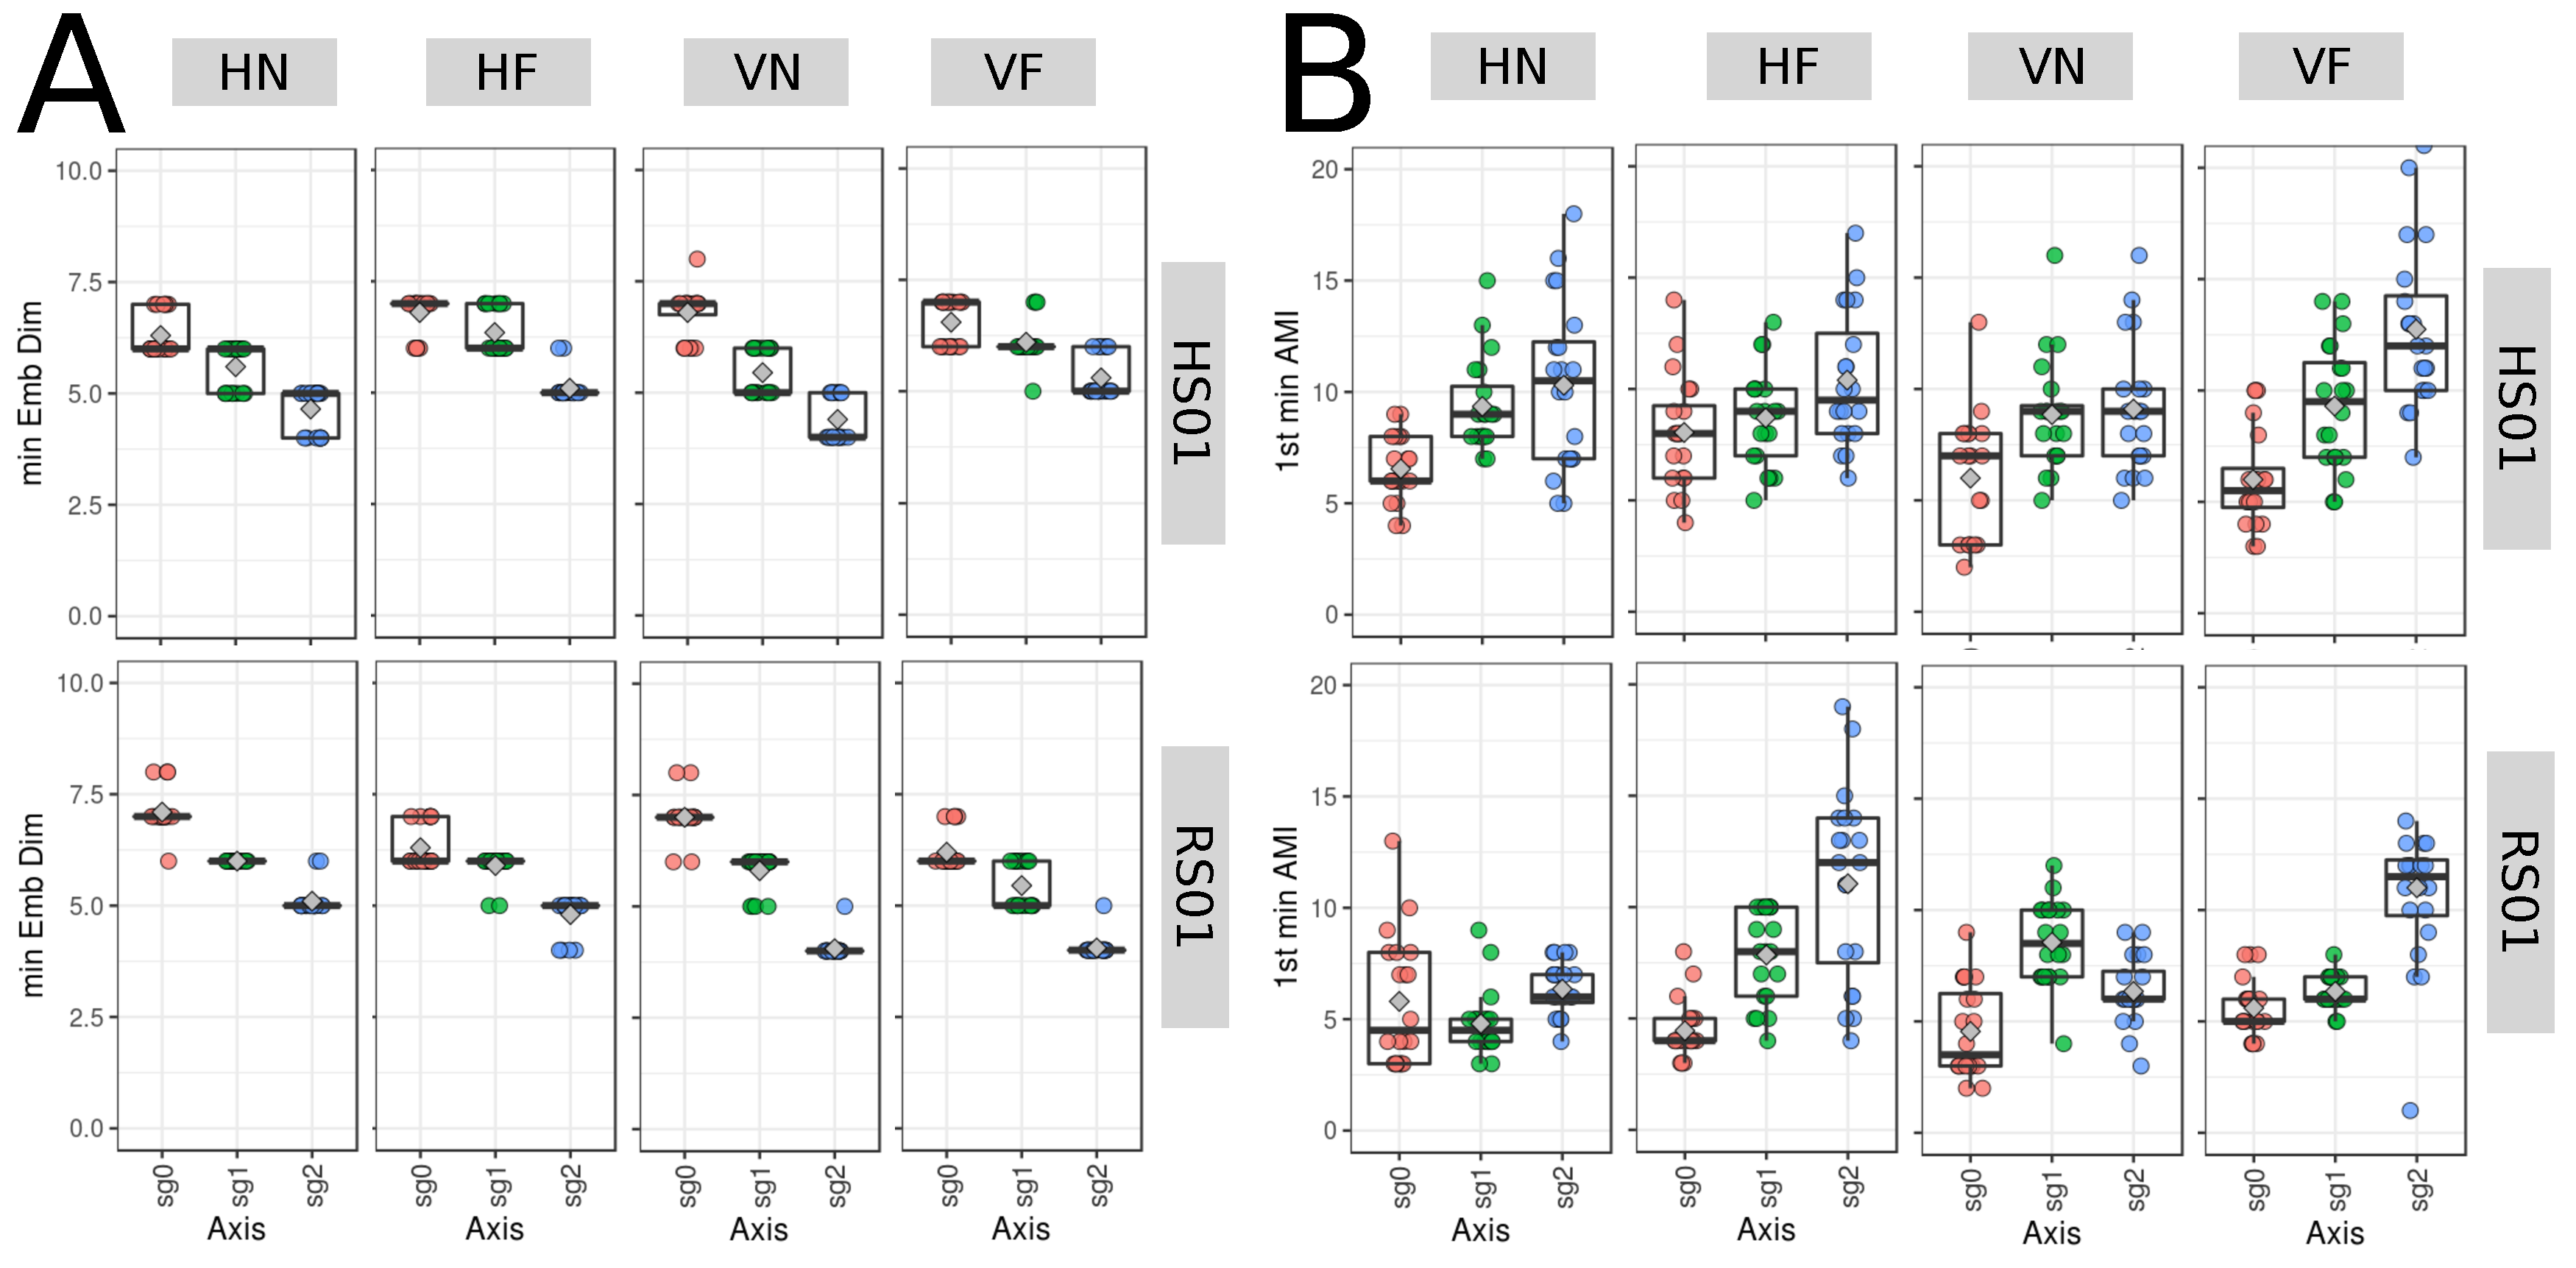
\includegraphics[width=1.0\textwidth]{fig-fig2.pdf}
	\caption{
	{\bf Box plots of minimum embedding parameters.} 
	Box plots of (A) minimum embedding dimensions 
	and (B) first minimum AMI values for 
	Horizontal Normal (HN), Horizontal Faster (HF),
	Vertical Normal (VN) and Vertical Faster (VF)
	with sensors attached to participants (HS01) and
	sensor attached to robot (RS01).
	Minimum embedding parameters are for twenty participants 
	($p01$ to $p20$) with three smoothed signals 
	(sg0: sg0zmuvGyroZ, sg1: sg1zmuvGyroZ and sg2: sg2zmuvGyroZ)
	and window length of 10-sec (500 samples).
	Code and data to reproduce the figure is available in \cite{srep2020}.
        }
    \label{fig:cao_ami}
\end{figure}
%%---------------------------------(FIGURE)------------------------------------

\subsubsection*{Uniform Time-Delay Embedding}
Using the overall embedding parameters ($\overline{m_0}=6$, $\overline{\tau_0}=8$), 
the first three axis of the rotated Principal Components Analysis (PCA) 
are shown for the reconstructed state spaces of horizontal (figures~\ref{fig:rsss}(A)) 
and vertical (figures~\ref{fig:rsss}(B)) arm movements. 
While visual inspection of these figures 
suggests differences in the trajectories of the reconstructed state spaces, 
we require an objective quantification to determine the extent of the differences.  
One approach could be use Euclidean distances from the origin for points in these 
trajectories, but this proved inconclusive and was not able to capture 
the dynamics of the trajectories. Consequently, we applied 
Recurrence Plots and Recurrence Quantification Analysis.
%%---------------------------------(FIGURE)-------------------------------------
\begin{figure}[ht]
\centering
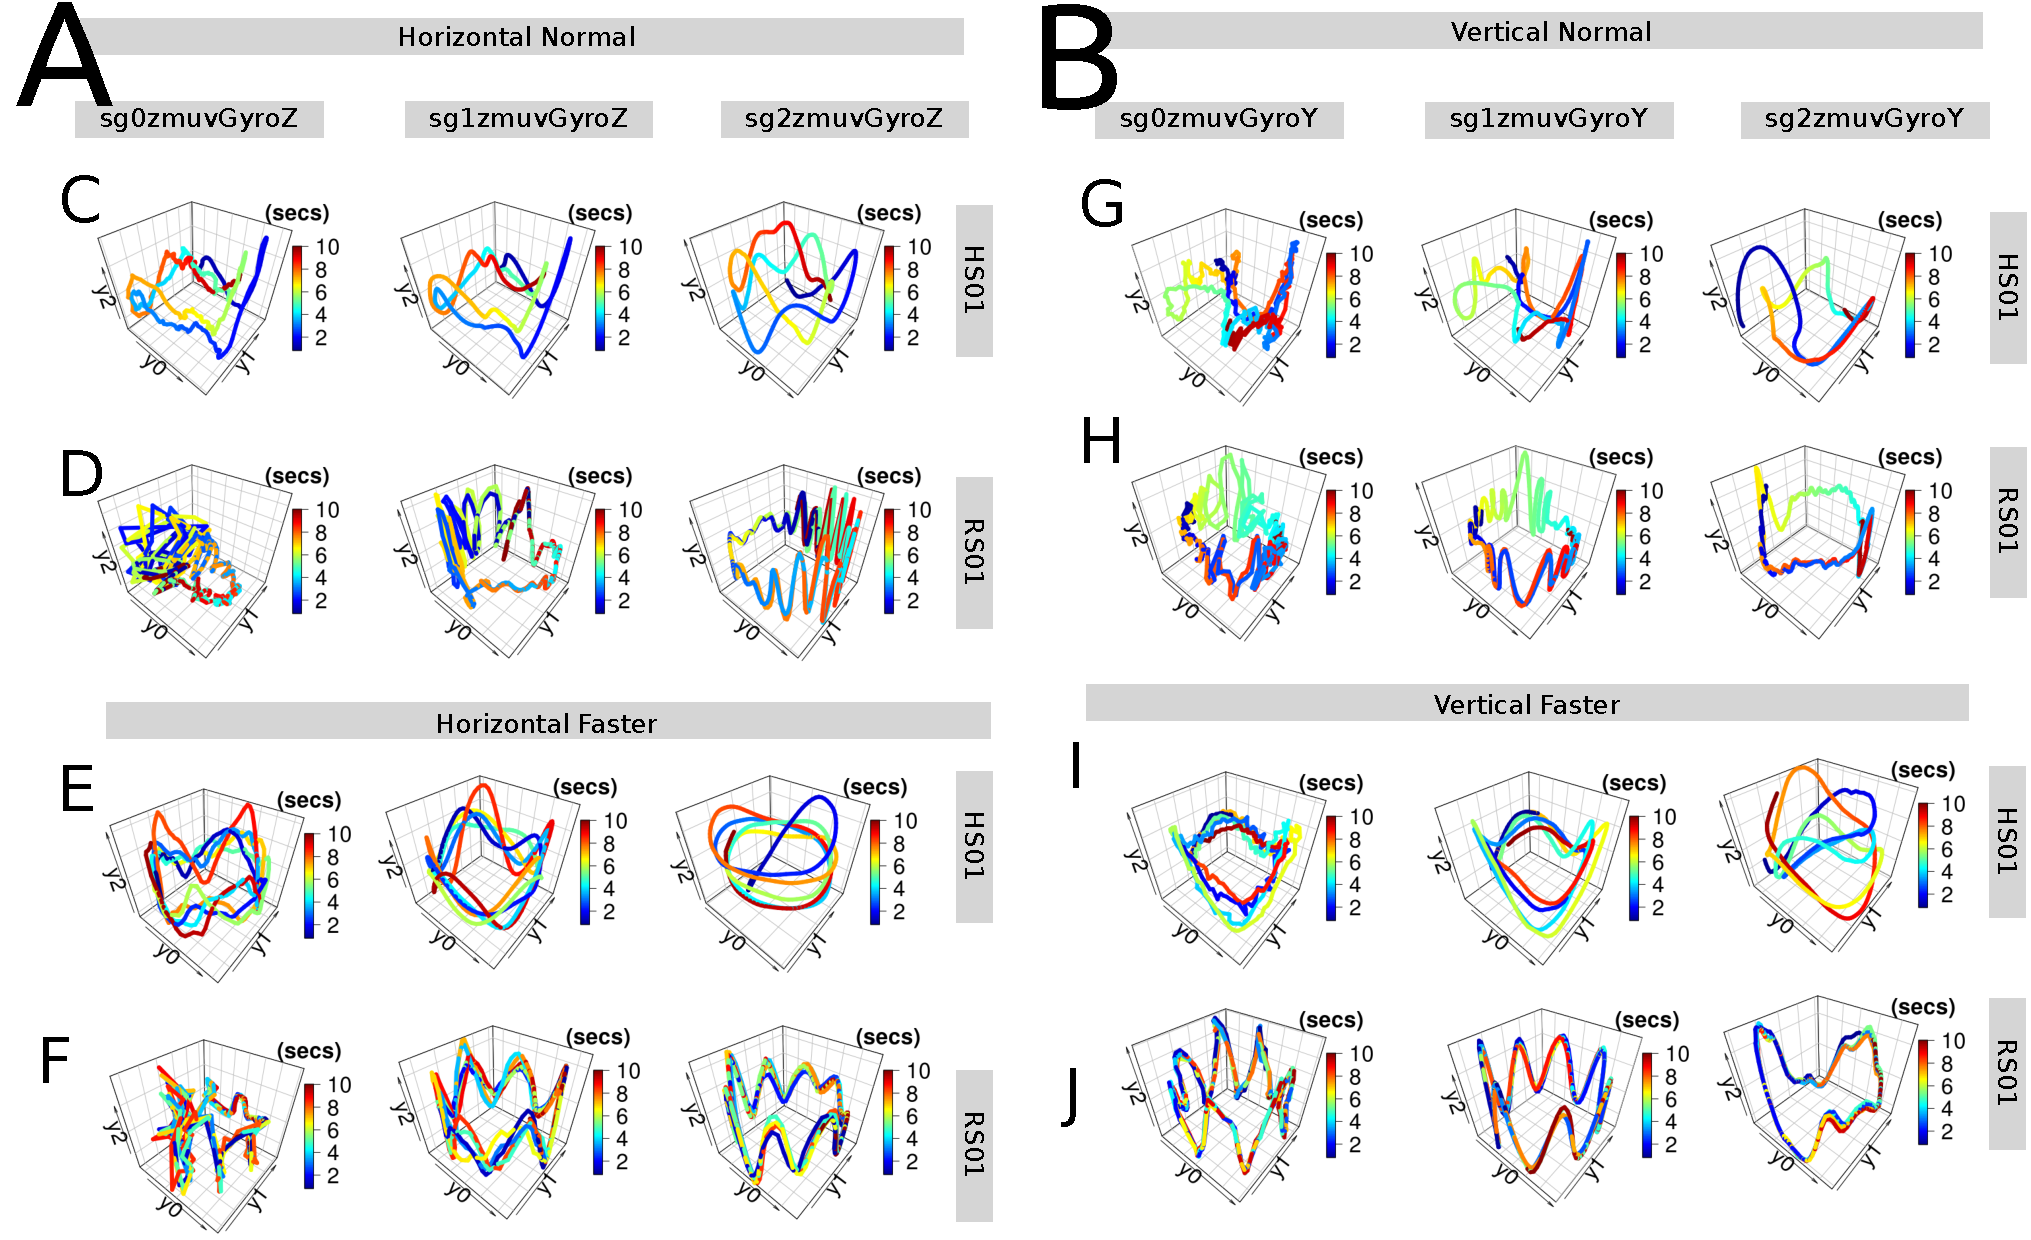
\includegraphics[width=1.0\textwidth]{fig-fig3.pdf}
\caption{
	{\bf RSSs for horizontal and vertical arm movements.}
	Reconstructed state spaces for time series for p01 of Figure \ref{fig:ts}.
	Reconstructed state spaces were computed with 
	embedding parameters 
	$\overline{m}_0=6$, $\overline{\tau}_0=8$
	for (A) horizontal and (B) vertical arm movements.
	Code and data to reproduce the figure is available in \cite{srep2020}.	
        }
    \label{fig:rsss}
\end{figure}
%%---------------------------------(FIGURE)------------------------------------



\subsection*{Recurrences Plots}
Using the average embedding parameters 
($\overline{m}_0=6$, $\overline{\tau}_0=8$) 
and an recurrence threshold of $\epsilon=1$.
As our interest is for dynamical transitions, 
there is little importance on the selection of $\epsilon$ which in this case
is 1. 
Recurrence Plots (RP) were computed for horizontal (figures~\ref{fig:rps}(A)) and 
vertical (figures~\ref{fig:rps}(B)) arm movements.
%%---------------------------------(FIGURE)-------------------------------------
\begin{figure}[ht]
\centering
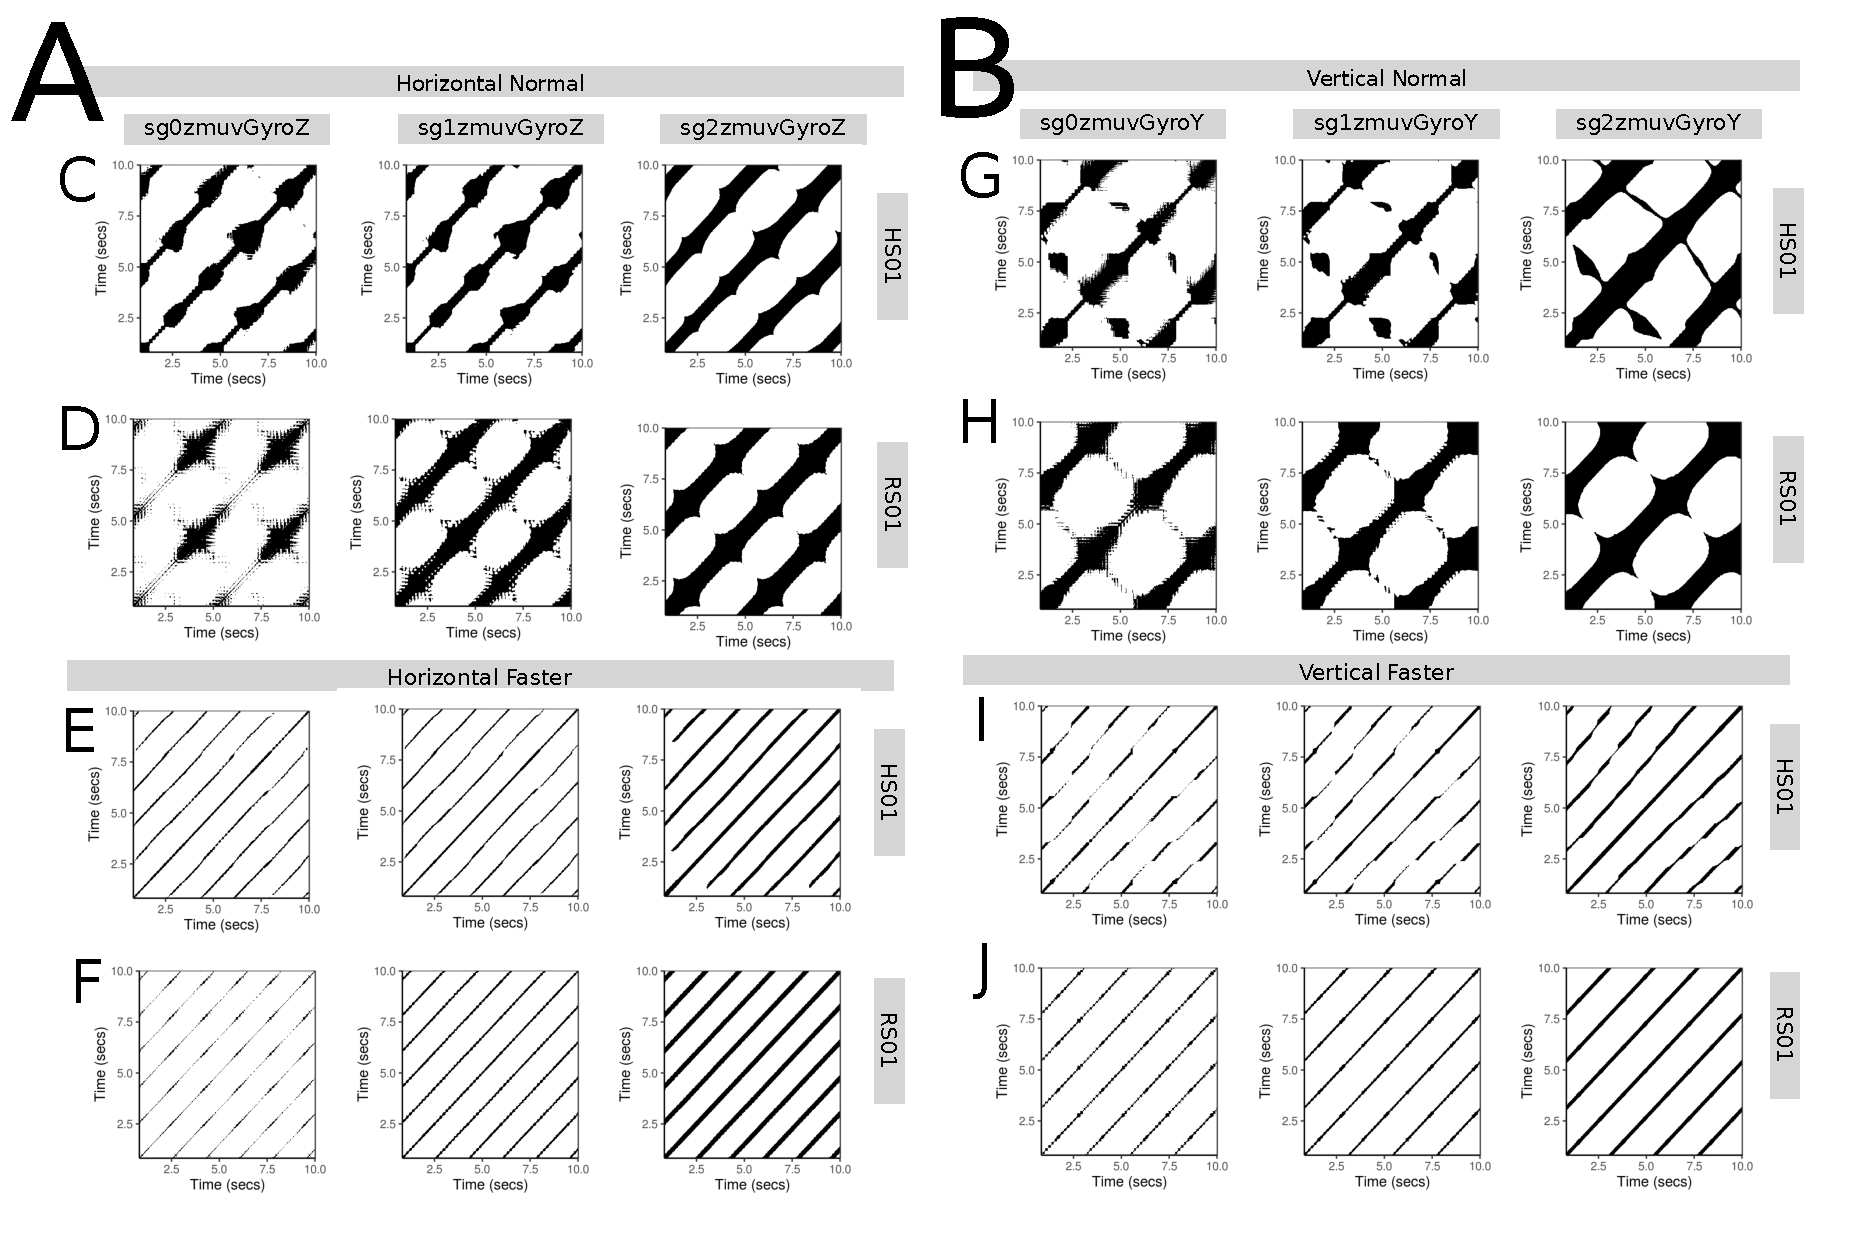
\includegraphics[width=1.0\textwidth]{fig-fig4.pdf}
\caption{
	{\bf RPs for horizontal (A) and vertical (B) arm movements.}	
	Recurrence plots were computed with 
	embedding parameters 
	$\overline{m}_0=6$, $\overline{\tau}_0=8$, and $\epsilon=1$.
	Code and data to reproduce the figure is available in \cite{srep2020}.
        }
    \label{fig:rps}
\end{figure}
%%---------------------------------(FIGURE)------------------------------------

\subsection*{Recurrence Quantification Analysis} \label{ch6:rqas}
Four Recurrence Quantification Analysis metrics (
percentage recurrence, REC, representing the percentage of black dots in RP; 
percentage determinism, DET, representing the predictability of the RP; 
ratio of DET / REC, RATIO; Shannon entropy, ENTR) 
were computed using the same parameters as for RP.
%\subsubsection*{REC values}
Figure~\ref{fig:RQABP}(A) presents box plots of REC values, 
for HS01, are more spread for Slow (i.e., 5 seconds per movement) movements 
in Horizontal (HS) or Vertical (VS) than for Fast (i.e., 2 seconds per movement).  
This suggests greater variation between participants for the Slow movements.  
For RS01, there is little variation between Slow and Fast movement
(interquartile range of 0.01). 
In terms of smoothness, there seems little effect of HS01 but RS01 values 
do show affects of smoothness (see the incremental changes of mean values (rhombus)).
%\subsubsection*{DET values}
Figure \ref{fig:RQABP}(B) presents DET values and shows 
little difference for type of movement or performer.  
However, DET values are affected by changes in smoothness of the signal, 
particularly for Fast movement.
%\subsubsection*{RATIO values}
Figure \ref{fig:RQABP}(C) presents the ratio of DET / REC. 
These values, for the human performer, vary less for HN than for HF movement.  
Additionally, smoothness leads to a decrease in mean values for Fast movements.
%\subsubsection*{ENTR values}
Figure \ref{fig:RQABP}(D) shows ENTR values are higher for the human 
performer than the robot, and vary with the smoothness of the time-series.
%%---------------------------------(FIGURE)-------------------------------------
\begin{figure}
\centering
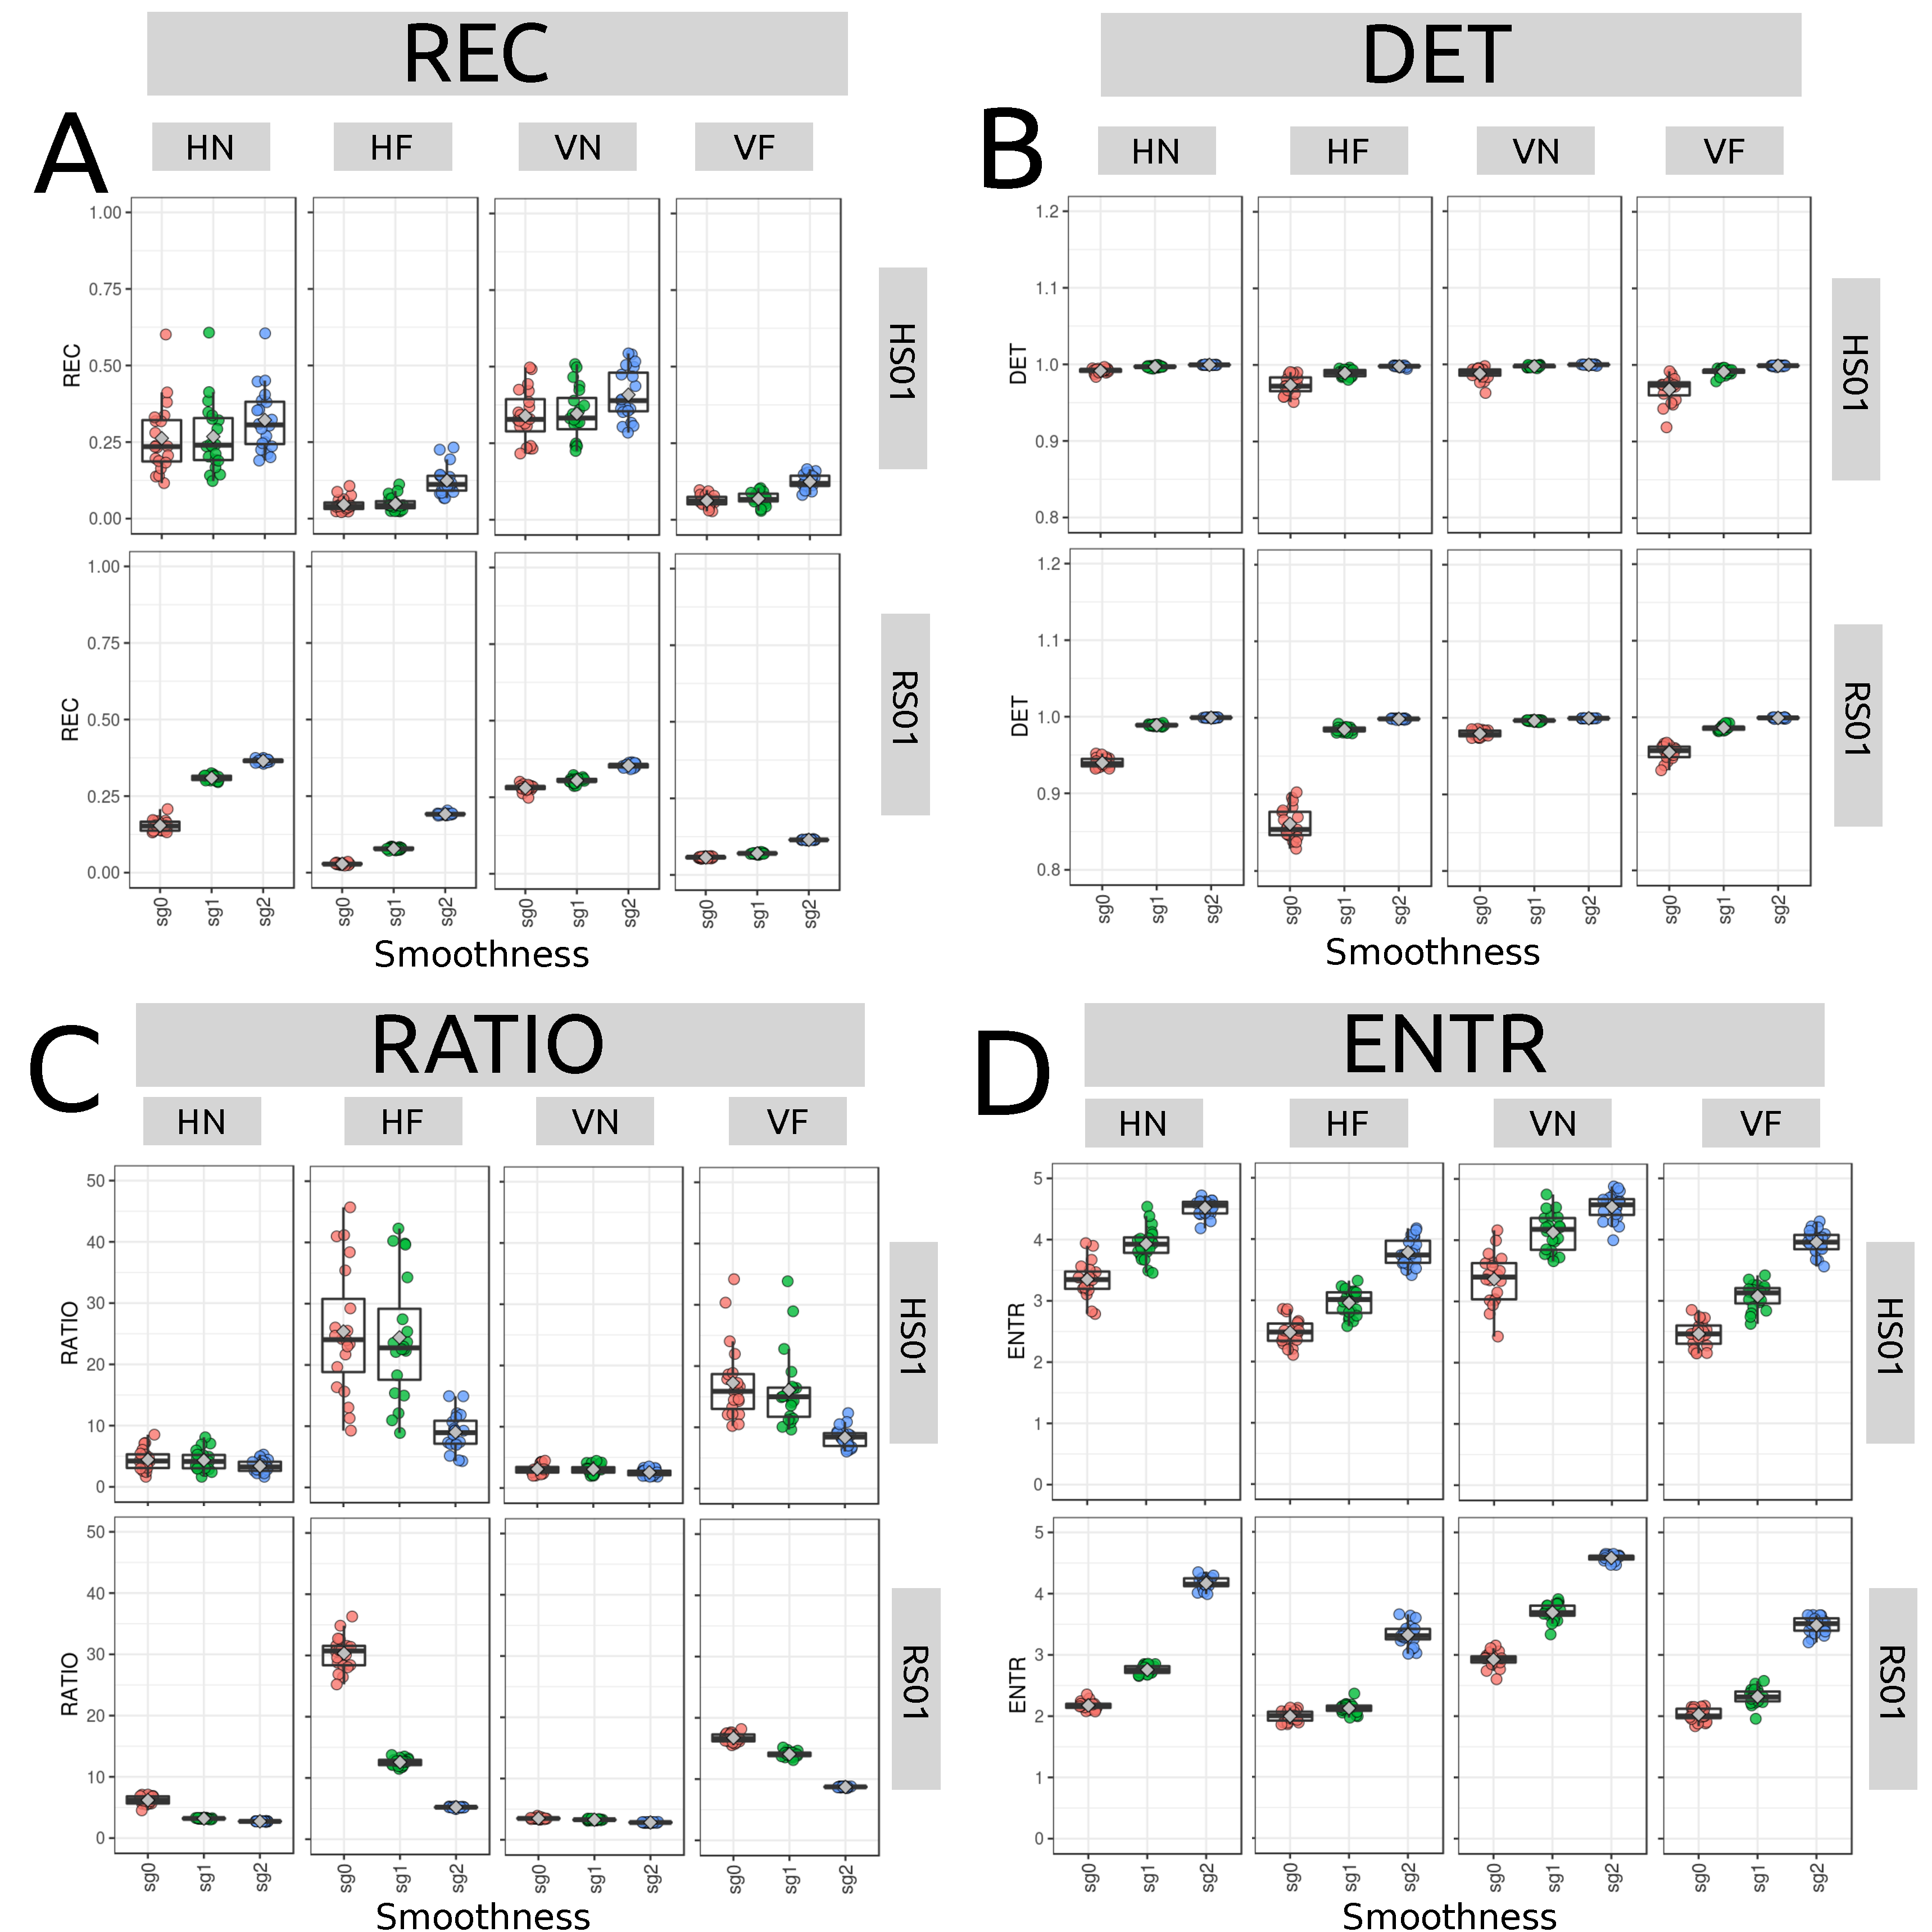
\includegraphics[width=1.0\textwidth]{fig-fig5.pdf}
    \caption
	[Box plots for RQA values]{
	{\bf Box plots for RQA metrics.}
	RQA metrics for (A) REC, (B) DET, (C) RATIO, and (D) ENTR of 
	20 participants performing HN, HF, VN and VF movements
	with sensors HS01, RS01 and three smoothed-normalised  
	time series (sg0, sg1 and sg2).
	RQA values were computed with 
	$\overline{m}_0=6$, $\overline{\tau}_0=8$, and $\epsilon=1$. 
	Code and data to reproduce the figure is available in \cite{srep2020}.
        }
    \label{fig:RQABP}
\end{figure}
%%---------------------------------(FIGURE)------------------------------------

%\subsection*{RQA metrics with fixed parameters}
%Considering that RQA metrics were computed with fixed embedding parameters 
%($m=6$ and $\tau=8$) and recurrence thresholds ($\epsilon=1$), we found 
%the following. REC values, which represents the \% of black points in the RPs, 
%were more affected with and increase in normal speed movements (HN and VN) 
%than faster movements (HF and VF) for the sensor attached to the participants 
%(HS01). Such decrease of REC values from normal speed to faster speed 
%movements is also presented in data from sensor attached to the robot (RS01), 
%and little can be said with regard to the dynamics of the time series coming 
%from RS01 (Fig \ref{fig:RQABP}A).
%Similarly, DET values, representing predictability and 
%organisation in the RPs, present little variation in the any of the time 
%series where little can be said (Fig \ref{fig:RQABP}B).
%In contrast, RATIO values, which represent 
%dynamic transitions, were more variable for faster movements (HF and VF) 
%than normal speed movements (HN and VN) with sensors attached to the 
%participants (HS01). For data coming from sensors attached to the robot 
%(RS01), RATIO values from horizontal movements (HN, HF) appear to vary 
%more than values coming from vertical movmentes (VN, VF) 
%(Fig \ref{fig:RQABP}C).
%With that, it can be said that RATIO values can represent a bit better
%than REC or DET metrics for the variability of imitation activities in 
%each of the conditions for time series.
%Similarly, ENTR values for HN were higher than values for HF
%and ENTR values varied more for sensor attached to participants 
%than ENTR values for sensors of the robot. It is evidently that 
%the higher the entropy the more complex the dynamics are, 
%however, ENTR values for HN appear a bit higher than HF values, 
%for which we believe this happens because of the structure the time series
%which appear more complex for HN than  HF movements which presented a 
%more consistence repetition (Fig \ref{fig:RQABP}D).


\subsection*{3D RQA ENTR}
As ENTR appeared to be have higher sensitivity than the other measures, 
we explored the impact of different embedding parameters 
$ \{ m \in \mathbb{R} | 1 \le m \le 10  \} $,
$  \{ \tau \in \mathbb{R} | 1 \le \tau \le 10  \} $ 
incrementing by 1 each run, with recurrence thresholds $\epsilon=1, 2, 3$ 
and levels of smoothness (sg0, sg1, sg2).  
Figure \ref{fig:RQA-IND} shows that increasing recurrence 
threshold leads to an increase in ENTR regardless of level of smoothness.  
Similarly, increasing level of smoothness will also increase ENTR (figure \ref{fig:RQA-IND}).
In terms of movement or performer, RQA ENTR decrease from Slow (HS, VS) to Fast (HF, VF) 
for both human (HS01) and (RS01) (Figures~\ref{fig:3dRQAENTR_sensoractivities}).
In terms of individual differences, for human participants, 
figure \ref{fig:3dRQAENTR_participantsactivities} compares p01, p02 and p03 (for illustrative purposes) --
both between each other and in comparison with the more consistent performance of the robot.  
In terms of window length (w100 (2s), w250 (5s), w500(10s), w750 (15s)), 
figure \ref{fig:3dRQAENTR_windowsactivities} shows that improvement in 
capture with number of samples, although this has less of an effect on RQA ENTR.

%%---------------------------------(FIGURE)-------------------------------------
\begin{figure}
\centering
\includegraphics[width=1.0\textwidth]{fig-rqa-epsilons.pdf}
    \caption
	[3D surface plots of RQA ENTR values]{
	{\bf 
	3D surface plots of RQA ENTR values for different recurrence threshold and smoothness levels.}
	RQA ENTR values are
	for embedding parameters
	$ \{ m \in \mathbb{R} | 0 \le m \le 10  \} $,
	$ \{ \tau \in \mathbb{R} | 0 \le \tau \le 10  \} $
	incrementing by one and three recurrence thresholds $\epsilon=1, 2, 3$.
	RQA ENTR values were computed with data from $p03$, sensor HS01, with 
	a window size of 10-secs (500 samples).
	Code and data to reproduce the figure is available in \cite{srep2020}.
        }
    \label{fig:RQA-IND}
\end{figure}
%%---------------------------------(FIGURE)------------------------------------

%%---------------------------------(FIGURE)-------------------------------------
\begin{figure}[ht]
\centering
\includegraphics[width=1.0\textwidth]{fig-rqa-sensors-activities.pdf}
    \caption{
	{\bf 3D surface plots of RQA ENTR values for different sensors and activities.}
	RQA ENTR values are for embedding parameters
	$ \{ m \in \mathbb{R} | 0 \le m \le 10  \}$,
	$ \{ \tau \in \mathbb{R} | 0 \le \tau \le 10  \}$
	with $\epsilon = 1 $ considering four activities 
	Horizontal Normal (HN), Horizontal Faster(HF), Vertical Normal(VN), and 
	Vertical Faster (VF) and sensors Human Sensor 01 (HS01) and 
	Robot Sensor (RS01).
	RQA ENTR values were computed from data of $p03$, sg0 and 
	window size of 10-secs (500 samples).
	Code and data to reproduce the figure is available in \cite{srep2020}.
       }
\label{fig:3dRQAENTR_sensoractivities}
\end{figure}
%%---------------------------------(FIGURE)-------------------------------------

%%---------------------------------(FIGURE)-------------------------------------
\begin{figure}[ht]
\centering
\includegraphics[width=0.9\textwidth]{fig-rqa-participants.pdf}
    \caption{
	{\bf 3D surface plots of RQA ENTR values for different participants, activities and sensors.}
	RQA ENTR values are for participants (p01, p02, and p03) 
	in the categories of 
	(A) Human Sensor 01 (HS01) and 
	(B) Robot Sensor 01 (RS01)
	considering embedding parameters
	$ \{ m \in \mathbb{R} | 0 \le m \le 10  \}$,
	$ \{ \tau \in \mathbb{R} | 0 \le \tau \le 10  \}$
	with $\epsilon = 1$ and four activities 
	Horizontal Normal (HN), Horizontal Faster(HF), Vertical Normal(VN), and 
	Vertical Faster (VF).
	RQA ENTR values were computed from data of sg0 and window size of 10-secs (500 samples).
	Code and data to reproduce the figure is available in \cite{srep2020}.
       }
\label{fig:3dRQAENTR_participantsactivities}
\end{figure}
%%---------------------------------(FIGURE)-------------------------------------

%%---------------------------------(FIGURE)-------------------------------------
\begin{figure}[ht]
\centering
\includegraphics[width=1.0\textwidth]{fig-rqa-windows}
    \caption{
	{\bf 3D surface plots of RQA ENTR values for different windows lengths and activities.}
	RQA ENTR values are for embedding parameters
	$ \{ m \in \mathbb{R} | 0 \le m \le 10  \}$,
	$ \{ \tau \in \mathbb{R} | 0 \le \tau \le 10  \}$, 
	with $\epsilon = 1 $ considering four 
	windows lengths (e.g., w100 (100 samples), w250 (250 samples),
	w500 (500 samples) and w750 (750 samples)) and
	four activities 
	Horizontal Normal (HN), Horizontal Faster(HF), Vertical Normal(VN), and 
	Vertical Faster (VF).
	RQA ENTR values were computed from data of $p01$ and sg0.
	Code and data to reproduce the figure is available in \cite{srep2020}.
       }
\label{fig:3dRQAENTR_windowsactivities}
\end{figure}
%%---------------------------------(FIGURE)-------------------------------------

To summarise this section of results, it can be said that computing
embedding parameters for individual structure of time-series 
data is already a solved problem \cite{frank2010, sama2013, bradley2015}. 
However, it has been shown the challenge of finding embedding parameters
for nonlinear dynamic tools that represent a set of different time-series data.
That said, we proposed the use of sample mean of the set of embedding parameters
for RSSs, RP and RQA to then noticed that the selection of recurrence 
threshold, $\epsilon$, is also an open problem.
For which, this work proposed the variation of recurrence thresholds 
and embedding parameters to show the relationships of these to different datasets 
(participants, activities, windows lengths and sensors).

%*******************************************************************************
%*******************************************************************************
%*******************************************************************************
\section*{Discussion}
While there are many approaches to estimating embedding parameters for nonlinear analysis, 
these can be influenced by the structure of the time-series data.   
We show that, for RSS, RP and RQA, the estimation of embedding parameters can be performed 
using a sample mean which, together with recurrence threshold, can be shown to be 
influenced by activity, performer, window length and smoothness of time-series.  
It is known that time-series from different sources and with different characteristics 
require different embedding parameters, and this can produce different RSS, RPs and RQAs. 
Although this work helps to understand the open problem of 
finding right balance among (i) the level of smoothness of the signal, 
(ii) the selection of recurrence thresholds and (iii) 
the range of embedding parameters, 
we have shown how RQA metrics can help to quantify movement variability.

\section*{Conclusions}
In this paper we show how the selection of nonlinear analysis tool  
(i.e., RSS, RP, RQA metrics) depends on what question one wishes to 
address with time-series data (e.g., predictability, organisation, dynamics, complexity).  
Time-series data characteristics (e.g., window length, smoothness), 
time-series structure (e.g., frequency, amplitude) and 
data source (e.g., sensor placement, performance, movement) all influence 
the results that nonlinear analysis methods can provide.
That said, it has been shown that the use of different characteristics of the data and 
their collection can help us visualise and quantify variability of movement using 
methods of nonlinear analysis.   
There remain limitations of nonlinear methods in 
relation to the estimation of parameters (e.g., recurrence threshold, embedding parameters) 
which reflect the dynamics of specific movement and performers, window length 
and structure of the time-series. 
We note that RQA DET seems to show low sensitivity 
to these differences, whereas REC and RATIO (primarily as a result of REC) show 
variation across performers and movements.   
RQA ENTR, with different recurrence thresholds, 
can quantify variation in the time-series data and offers the most appropriate means 
for analysing variability in movement to allow us to analyse individual differences 
between human performers.  
To then found out that RQA ENTR values with different recurrence 
thresholds were appropriate to quantify 
the different changes and variations of the characteristics of 
time-series data.
Therefore, the use of Shannon Entropy could be applied 
to analyse human participants who might vary in age, 
state of health, anthropometric features and capability to perform movement.

%% As a guideline references should be limited to 60 (this is not 
%% strictly enforced).
%\bibliography{sample}
%\bibliography{../references/references}
%\bibliography{references}
%*******************************************************************************
\documentclass[fleqn,10pt]{wlscirep}
\usepackage[utf8]{inputenc}
\usepackage[T1]{fontenc}
%\graphicspath{{../}} %goes to path: docs/

\title{Nonlinear methods to quantify Movement Variability in Human-Humanoid Interaction Activities}
\author[1,*]{Miguel Xochicale}
\author[2]{Chris Baber}
\affil[1]{King's College London, 
	School of Biomedical Engineering amd Imaging Sciences,
	London, SE1 7EU, UK
	} 
\affil[2]{University of Birmingham,
	School of Computer Science,
	Birmingham, 
	B15 2TT, 
	UK}
\affil[*]{miguel.xochicale@kcl.ac.uk}


%\keywords{Keyword1, Keyword2, Keyword3}

\begin{abstract}
Human movement variability arises from the process of 
mastering redundant (bio)mechanical degrees of freedom (DOF)
to successfully accomplish any given motor task
(from the most complex to even the simplest one) 
where flexibility and stability of many possible joint 
combinations helps to adapt to environment conditions. 
While the analysis of movement of variability is becoming increasingly 
popular as a diagnostic tool or skill performance evaluation, 
there are remain challenges in terms of defining 
the most appropriate methods and parameters to apply. 
For this work, we therefore investigate nonlinear dynamics methods 
such as reconstructed state space (RSSs), uniform time-delay embedding, 
recurrence plots (RPs) and recurrence quantification analysis metrics (RQAs)
with real-world time-series data of wearable inertial sensors. 
That said, twenty right-handed healthy participants 
imitated simple vertical and horizontal arm movements in normal 
and faster velocity from an humanoid robot.
We applied nonlinear methods to four activities, 
four window lengths and three levels of smoothed time-series data,
to then found visual differences in the patterns of RSSs and RPs
and statistical differences with RQA metrics.
We therefore conclude that Shannon Entropy for RQA is a robust method 
that help us to quantify activities, types of sensors, windows lengths 
and level of smoothness.
Hence this work might enhance the development of 
better diagnostic tools for applications in 
rehabilitation and sport science for skill performance
or new forms of human-humanoid interaction for
quantification of movement adaptations and motor pathologies.
\end{abstract}


\begin{document}
\flushbottom
\maketitle
\thispagestyle{empty}

\section*{Introduction}
The complexity of human movement arises from the process of mastering 
redundant (bio)mechanical degrees of freedom (DOF) to successfully 
accomplish any given motor task (Bernstein, 1967).
Such DOF are independent coordinates to uniquely 
describe the configurations of the system which provides flexibility 
and stability to adapt to a change environment conditions but 
that leads many possible combinations (Newell and Vaillancourt, 2001).
Hence, human movement complexity can be seen as a balance 
between the required DOF "to generate a stable (persistent) 
and flexible (variable) behavioural output in response to 
changing intentions and dynamic environmental
conditions" \cite{davids2003}. 
Consequently, one can see much variability in human movement even in the 
simplest of movements.  
While the analysis of movement of variability is becoming increasingly 
popular as a diagnostic tool or skill performance evaluation, 
there remain challenges in terms of defining 
the most appropriate methods and parameters to apply. 
In part, 
these challenges stem from the fact that the identification movement 
variability requires analysis of signals which are time-series of 
of $1-$dimension in $\mathbb{R}$ which are 
noisy, nonlinear and non-stationary \cite{gomezgarcia2014}.
Further problems arise from assigning a plausible locus of control to 
the movements, e.g., in order to determine whether variability is the 
result of deliberative control by the performer or whether it arises 
from exogenous or endogenous disturbances.  For this paper, our focus 
is on the analysis of signals; specifically, in terms of objectively 
quantifying variability of lower dimension signals using time-series analysis.

Methods for nonlinear time series analysis generally involve the estimation of the 
embedding parameters ($m$ embedding dimension and $\tau$ embedding delay) to 
reconstruct the state space,
where an $n$-dimensional is reconstructed state space using $1-$dimensional 
time series \cite{Quintana-Duque2012, Quintana-Duque2016, sama2013, 
frank2010, gomezgarcia2014, marwan2011, stergiou2011}.
Key to the selection of these parameters is the need to preserve 
topological properties of an unknown $M$-dimensional state space \cite{takens1981}.
An common approach to the construction of these state spaces 
involves Recurrence Plots (RPs), a graphical representation of black and white dots, 
which shows recurrent patterns of a $n$-dimensional system.
While RPs provide a human
interpretable picture of the system, these require further
analysis to allow the properties of that system to be quantified,
and so Recurrence Quantification Analysis (RQA) can be applied.
However, the estimation of the embedding parameters for
RQA remains an open problem (Bradley et al. 2015 \cite{bradley2015})
There is no agreed method to estimate embedding parameters
for RQA and other nonlinear methods \cite{bradley2015} 
because time series are system-dependent, i.e., these rely
on the initial conditions, and on the configuration and behaviour of the system.  
This means that, unless one holds all of the influencing 
variables constant, embedding parameters computed for one 
instance may not apply to another instance.   

One could apply methods, such as autocorrelation, mutual information, 
nearest neighbour (and we will apply these in this paper), 
but these methods assume that the data are well sampled, with 
little noise and (usually) that the signals are purely deterministic \cite{garland2016, kantz2003}.
That said, these methods can break-down in the face of real-world datasets 
which could have 
different length, 
different values of accuracy and precision (rounding errors due to finite 
precision of the measurement apparatus which include frequency 
acquisition \cite{frank2010}), or 
different levels of contamination from exogenous and endogenous 
sources of ‘noise’ \cite{garland2016}.  What is, perhaps, surprising is that 
even subject to these problems, the methods are useful and 
nonlinear dynamics approaches continue to tell us much about 
human movement \cite{Quintana-Duque2012, Quintana-Duque2016, sama2013, frank2010,
gomezgarcia2014, marwan2011, stergiou2011, bradley2015}.

For this paper, we explore the role of RPs and RQA in the 
analysis of simple human movement. 
We compare horizontal and 
vertical arm movements performed by neurotypical participants 
who are copying these movements being made by a humanoid robot.  
This provides an initial point of comparison 
(between human movement, which we assume to have a degree of variability, 
and the robot, which we assume to have a degree of consistency).   
Additionally, our interest lies in the estimation of embedding parameters 
in light of different features of the data, e.g., levels of smoothing, 
window length, structure of time-series based on movement, 
types of sensors, individual differences between participants and 
the movements that they perform. 
Specifically, we ask what are 
the effects of different embedding parameters, recurrence thresholds 
and characteristics of time-series on nonlinear analysis 
methods (i.e., reconstructed state space with 
uniform time-delay embedding, RPs and RQA)?



%*******************************************************************************
%*******************************************************************************
%*******************************************************************************
\section*{Methods}
\subsection*{State Space Reconstruction}
The method of state space reconstruction \cite{packard1980} 
\cite{takens1981} has been applied in many disciplines 
\cite{aguirre2009, stergiou2011, frank2010, 
sama2013, Quintana-Duque2016}. The method of state space reconstruction is 
based on uniform time-delay embedding methodology which is a simple 
matrix implementation that can reconstruct an unknown $d-$dimensional 
manifold $M$ from a scalar time series (e.g. one-dimensional 
time series in $\mathbb{R}$). A manifold, in this context, is a 
multidimensional curved surface within a space (e.g. a saddle) 
\cite{guastello-gregson2011}.

The use of a scalar time series is the main advantage of the method of state 
space reconstruction which in essence preserve dynamic invariants such as 
correlation dimension, fractal dimension, Lyapunov exponents, Kolmogorov-Sinai 
entropy and detrended fluctuation analysis \cite{bradley2015, 
Quintana-Duque2012, Quintana-Duque2013, Quintana-Duque2016, krakovska2015}.
However, selecting appropriate embedding parameters which are sued to apply the 
state space reconstruction is still an open challenge for which we present 
introductions for the methodologies to compute such embedding parameters 
With that in mind, in the following subsections, we describe in more detail 
the state space reconstruction theorem (RSSs), uniform time-delay embedding 
theorem (UTDE), false nearest neighbours (FNN) and average mutual 
information (AMI). 
%and other methodologies for state space reconstruction.

\subsection*{State Space Reconstruction Theorem}
Following the notation employed in \cite{casdagli1991, garland2016, gibson1992,
uzal2011, uzal2010, takens1981}, state space reconstruction is defined by:
%%********************************[EQUATION]************************************
\begin{equation}\label{eq:ssr}
  s(t)=f^t [s(0)],
\end{equation}
%%********************************[EQUATION]************************************
where $s$, $s: A \rightarrow M$ given that $A \subseteq \mathbb{R}$ and 
$M \subseteq \mathbb{R}^d$, represents a trajectory which evolves in an 
unknown $d-$dimensional manifold $M$, $f: M \rightarrow M$ is an evolution 
function and $f^t$, with time evolution $t \in \mathbb{N}$, is the $t$-th 
iteration of $f$ that corresponds to an initial position 
$s(0) \in M $ \cite{takens1981}.
%$f$ is a smooth dynamical system, where smooth means a 
%continuously differentiable system
%(e.g. derivatives exist at all points) \cite{guastello-gregson2011}.
Then, a point of a one-dimensional time series $x(t)$ in $\mathbb{R}$, 
can be obtained with
%%********************************[EQUATION]************************************
\begin{equation}\label{eq:measurement}
  x(t)=h[s(t)],
\end{equation}
%%********************************[EQUATION]************************************
where $h$ is a function, $h: M \rightarrow \mathbb{R}$, defined on the trajectory $s(t)$.
Reconstructed state space can then be described as an $n-$dimensional state 
space defined by $y(t)=\Psi[\boldsymbol{X}(t)]$ where 
$\boldsymbol{X}(t) = \{ x(t), x(t-\tau) , ...,x(t - (m-1)\tau  ) \}$ 
is the uniform time-delay embedding with a dimension embedding $m$
and delay embedding $\tau$ and
$ \Psi: \mathbb{R}^m \rightarrow \mathbb{R}^n$ is a further transformation
of dimensionality (e.g. Principal Component Analysis, 
Singular Value Decomposition, etc) being $n \leq m$.
With that in mind, uniform time-delay embedding, $\boldsymbol{X}(t)$, 
defines a map $\Phi: M \rightarrow \mathbb{R}^m$ such that 
$\boldsymbol{X}(t) = \Phi(s(t))$,
where $\Phi$ is a diffeomorphic map \cite{takens1981}
whenever $\tau > 0$ and $m > 2d_{box}$ and $d_{box}$ is the box-counting
dimension of $M$ \cite{garland2016}.
% "Given two manifolds $M$ and $N$, a differientiable map $f: M \rightarrow N$
% is called diffeomorphic if it is one-to-one correspondence and its inverse
% $f^{-1}: N \rightarrow M$ is differientiable as well \cite{wiki:diffeomorphic}".
Then, if $\Phi$ is an embedding of evolving trajectories in the reconstructed 
space then a composition of functions represented with $F^t$ is induced on the
reconstructed state space determined:
%by true smooth dynamical system $f^t$ and $\Phi$:
%********************************[EQUATION]************************************
\begin{equation}\label{eq:st}
  \boldsymbol{X}(t)=F^t [\boldsymbol{X}(0)] = \Phi \circ f^t \circ \Phi ^{-1}[\boldsymbol{X}(0)].
\end{equation}
%%********************************[EQUATION]************************************
With this in mind, an embedding is defined as "a smooth one-to-one 
coordinate transformation with a smooth inverse" and the total reconstruction 
map is defined as $ \Xi = \Psi \circ \Phi $ \cite{casdagli1991}.
Fig~\ref{fig:ssr} illustrates the state space reconstruction.
%%---------------------------------(FIGURE)-------------------------------------
\begin{figure}[ht]
\centering
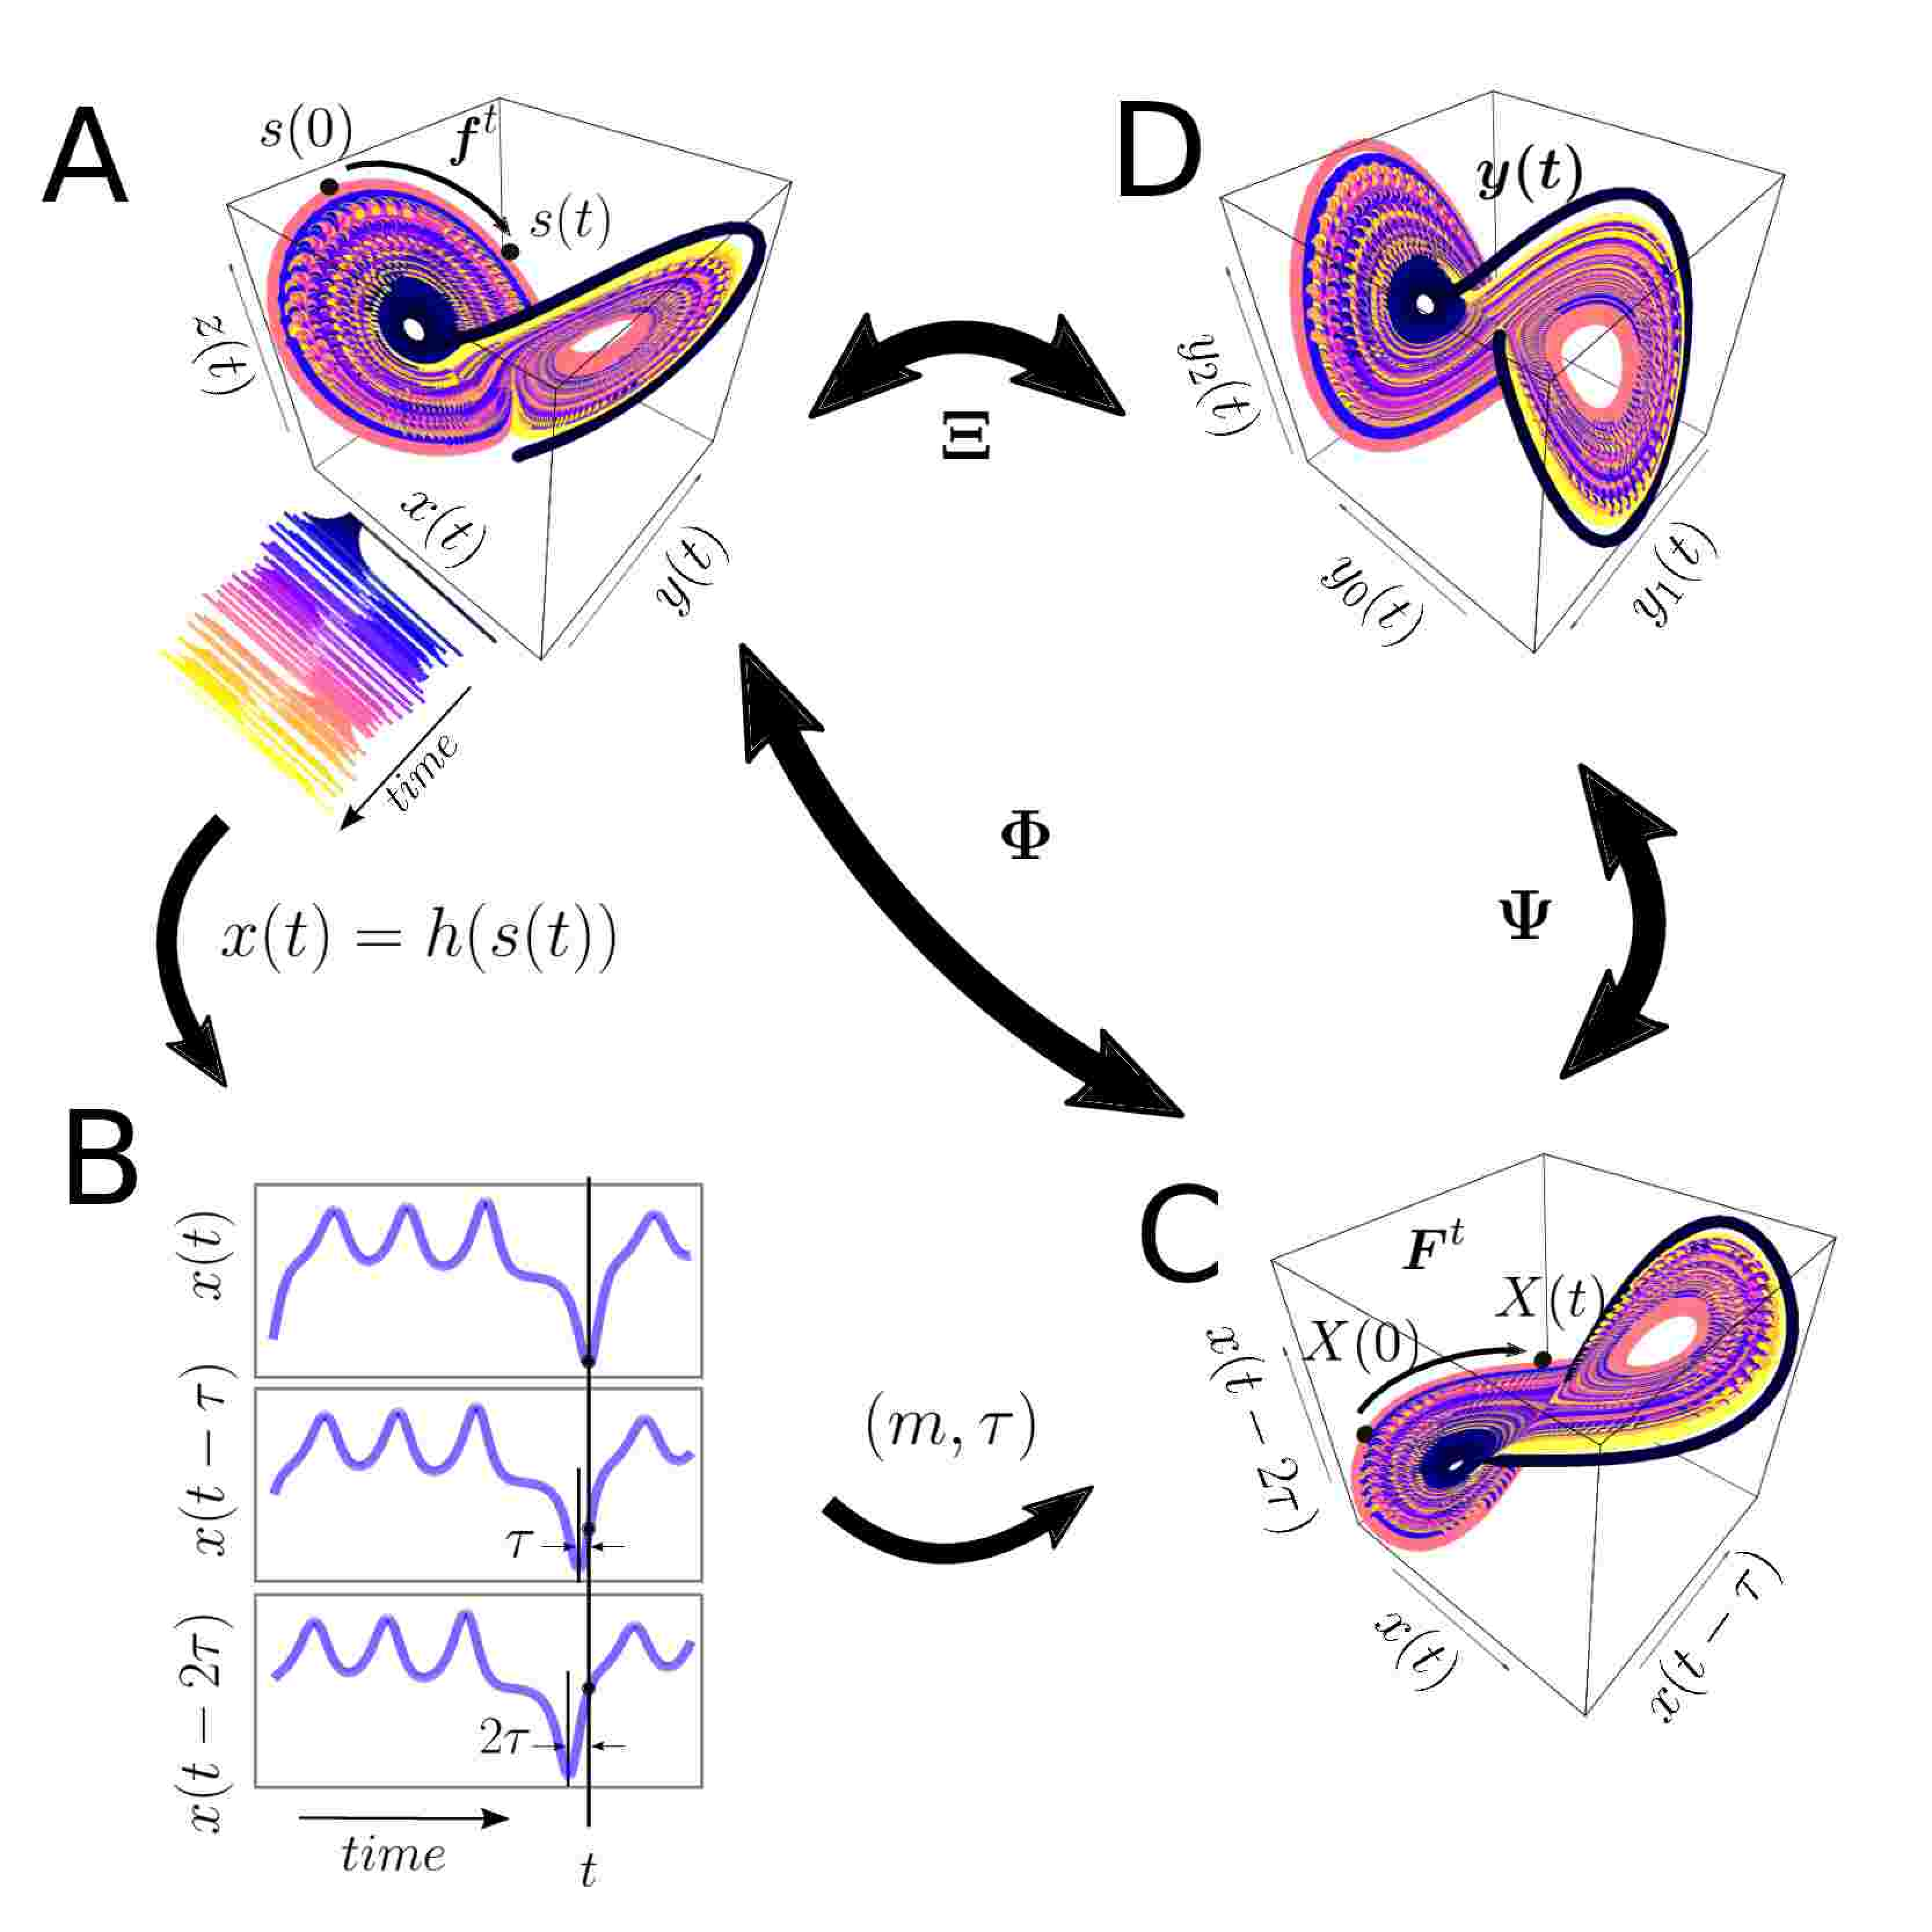
\includegraphics[width=1.0\textwidth]{fig-rss.pdf}
    \caption{
	{\bf State space reconstruction methodology.}
	State space reconstruction is based on $x(t)=h[s(t)]= h[f^t [s(0)]]$
	where $f^t$ is the true dynamical system, $s(t)$ indicates the state,
    	$s$, at time, $t$,  and $h[ ]$ the measurement function. 
    	The time-delay embedding represented as the $\Phi$, maps the original
    	$d-$dimensional state $s(t)$ into the $m-$dimensional uniform 
	time-delay embedding matrix $\boldsymbol{X}(t)$.
    	The transformation map $\Psi$ then maps $\boldsymbol{X}(t)$ into 
	a new state $y(t)$ of dimensions $n < m$.
    	(A) $M-$dimensional manifold representing the state space 
	(e.g. Lorenz system);
    	(B) Delayed copies of $1-$dimensional $x(t)$ from the Lorenz system;
   	(C) $m-$dimensional reconstructed state space with 
    	\texorpdfstring{$m$}{m} and    \texorpdfstring{$\tau$}{T}, and 
    	(D) $y(t)$ is the $n-$dimensional reconstructed state space.
	The total reconstruction map is represented as $\Xi = \Psi \circ \Phi $
	where $\Phi$ is the delay reconstruction map and 
	$\Psi$ is the coordinate transformation map.
	This figure is adapted from 
   	\cite{Quintana-Duque2012, casdagli1991, uzal2011}.
	Code and data to reproduce the figure is available in \cite{srep2020}.
    }
    \label{fig:ssr}
\end{figure}
%%---------------------------------(FIGURE)-------------------------------------



\subsection*{Uniform Time-Delay Embedding (UTDE)}\label{sec:utimedelayembedding}
Frank et al. and Sama et al. refer to the state space reconstruction
as "time-delay embeddings" or "delay coordinates" \cite{frank2010, sama2013}. 
However, we consider the term "uniform time-delay embedding"
as more descriptive and appropriate terminology for our work.
Hence, the uniform time-delay embedding is represented as a matrix of uniform delayed 
copies of the time series $\{ \boldsymbol{x}_n \}_{n=1}^N$ where $N$ is 
the sample length of $\{ \boldsymbol{x}_n \}$ and $n$ is index for the 
samples of $\{ \boldsymbol{x}_n \}$.
$\{ \boldsymbol{x}_n \}_{n=1}^N$ has a sample rate of $T$.
The delayed copies of $\{ \boldsymbol{x}_n \}$ are uniformly separated by $\tau$
and represented as $\{\boldsymbol{ \tilde{x} }_{n- i\tau} \}$
where $i$ goes from $0,1, \dots, (m-1)$.
Generally speaking, $\{\boldsymbol{ \tilde{x} }_{n- i\tau} \}$ contains
information of unobserved state variables and encapsulates the information of
the delayed copies of the available time series in the uniform time-delay 
embedding matrix $\boldsymbol{X}^{m}_{\tau}$, 
$\boldsymbol{X}^{m}_{\tau} \in \mathbb{R}^m$, defined as
%%********************************[EQUATION]************************************
\begin{equation}\label{eq:tde}
\boldsymbol{X}^{m}_{\tau}  =
\begin{pmatrix}
\boldsymbol{ \tilde{x} }_n \\
\boldsymbol{ \tilde{x} }_{n-\tau} \\
\boldsymbol{ \tilde{x} }_{n-2\tau} \\
\vdots \\
\boldsymbol{ \tilde{x} }_{n- (m-1) \tau} \\
\end{pmatrix}^\intercal, 
\end{equation}
%%********************************[EQUATION]************************************
where $m$ is the embedding dimension, $\tau$ is the embedding delay and
$ ^\intercal$ denotes the transpose.
$m$ and $\tau$ are known as embedding parameters.
The matrix dimension of $ \boldsymbol{X}_{\tau}^{m} $ is defined by
$N-(m-1)\tau$ rows and $m$ columns and 
$N-(m-1)\tau$ defines the length of each delayed copy 
of $\{ \boldsymbol{ \tilde{x} }_n \}$ in $\boldsymbol{X}^{m}_{\tau}$.
%For further details and explicit examples of uniform time-delay 
%embedding methodology, we refer the reader to the \nameref{S1_AppendixA}.




\subsection*{Estimation of Embedding Parameters}
The estimation of the embedding parameters ($m$ and $\tau$) 
is a fundamental step for the state space reconstruction with the use
of uniform time-delay embedding method.
With this in mind, we review two of the most common algorithms,
which will be used in our work, to compute the embedding
parameters: the false nearest neighbour (FNN) and the average mutual information (AMI).

%%%%%%%%%%%%%%%%%%%%%%%%%%%%%%%%%%%%%%%%%%%%%%%%%%%%%%%%%%%%%%%%%%%%%%%%%%%%%%%%
%*******************************************************************************
\subsubsection*{False Nearest Neighbours}
To select the minimum embedding dimension $m_0$, Kennel et al. \cite{kennel1992}
used the method of false neighbours which can be understood as follows:
on the one hand, when the embedding dimension is too small to unfold the 
attractor "not all points that lie close each other will be neighbours and 
some points appear as neighbours because of the attractor has been projected 
down into an smaller space", on the other hand, when increasing the embedding 
dimension "points that are near to each other in the sufficient
embedding dimension should remain close as the dimension increase from $m$ 
to $m+1$ \cite{krakovska2015}".
From a mathematical point of view, the state space reconstruction theorem is 
done when the attractor is unfolded with either the minimum embedding 
dimension, $m_0$, or any other embedding dimension value where 
$m \ge m_0$ \cite{kennel1992}. On the contrary, any large value of $m_0$ 
leads to excessive computations \cite{bradley2015}. With this in mind, 
Cao \cite{Cao1997} proposed an algorithm based on the false neighbour method 
where only the time-series and one delay embedding value are necessary 
to select the minimum embedding dimension. Cao's algorithm is based 
on $E(m)$  which is the mean value of all $a(i,m)$, both defined as follows
%%********************************[EQUATION]************************************
\begin{equation}\label{eq:e}
  \begin{aligned}
	E(m) &= \frac{1}{N-m\tau} \sum_{i=1}^{N-m\tau} a(i,m) \\
	 &=
       \frac{1}{N-m\tau} \sum_{i=1}^{N-m\tau}
       \frac{ || \boldsymbol{X}_i(m+1) - \boldsymbol{X}_{n(i,m)}(m+1) || }
            { || \boldsymbol{X}_i(m) - \boldsymbol{X}_{n(i,m)}(m) ||  }
  \end{aligned}
\end{equation}
%%********************************[EQUATION]************************************
where $\boldsymbol{X}_i(m)$ and $\boldsymbol{X}_{n(i,m)}(m)$ are the time-delay
embeddings with $i=1,2,\dots,N-(m-1)\tau$ and $ n(i,m)= 1 \le n(i,m) \le N-m\tau$.
From Eq.~\ref{eq:e}, it can be seen that $E(m)$ is only dependent on $m$ 
and $\tau$ for which $E_1(m)$ is defined as
%%********************************[EQUATION]************************************
\begin{equation}\label{eq:e1}
E_1(m) = \frac{ E(m+1) } { E(m)}.
\end{equation}
%%********************************[EQUATION]************************************
$E_1(m)$ is therefore considered to investigate the variation from $m$ to $m+1$
in order to find the minimum embedding dimension $m_0$ (Eq.~\ref{eq:e1}).
As described in \cite{Cao1997}: "$E_1(m)$ stops changing when $m$ is greater
than some $m_0$, if the time series comes from a multidimensional state space
then $m_0 + 1$ is the minimum dimension".
Additionally, Cao proposed $E_2(m)$ to distinguish deterministic signals from
stochastic signals. $E_2(m)$ is defined as
%%********************************[EQUATION]************************************
\begin{equation}\label{eq:e2}
E_2(m) = \frac{ E^* (m+1) } { E^*(m)},
\end{equation}
%%********************************[EQUATION]************************************
where
%%********************************[EQUATION]************************************
\begin{equation}\label{eq:ee}
E^*(m) = \frac{1}{N-m\tau} \sum_{i=1}^{N-m\tau}
|  \boldsymbol{X}_i(m+1) - \boldsymbol{X}_{n(i,m)}(m+1) |.
\end{equation}
%%********************************[EQUATION]************************************
For instance, when the signal comes from random noise (values that are 
independent from each other), all $E_2(m)$ values are approximately equal 
to 1 (e.g. $E_2(m) \approx 1$). However, for deterministic data $E_2(m)$ is 
not constant for all $m$ (e.g. $E_2(m) \neq 1$).

As an example of the use of $E_1(m)$ and $E_2(m)$ values, we consider two time 
series: the solution for the $x$ variable of the Lorenz system 
(Fig~\ref{fig:caoami}A), and a Gaussian noise time series with zero mean 
and a variance of one (Fig~\ref{fig:caoami}B).
We then compute $E_1(m)$ and $E_2(m)$ values for each time series.
The $E_1(m)$ values for the chaotic time series appear to be constant
after the dimension is equal to six.
The determination of six is given that any value of $m$ can be used as they 
are within the threshold of $1\pm0.05$ (Fig~\ref{fig:caoami}C).
$E_2(m)$ values, for chaotic time series, are different to one 
(Fig~\ref{fig:caoami}E), for which, it can be concluded that for the 
chaotic time series the minimum embedding dimension the time series 
comes from a deterministic signal. With regard to the noise time series,  
$E_1(m)$ values appeared to be constant when $m$ is close to thirteen, 
which is defined by the threshold of $1\pm0.05$ (Fig~\ref{fig:caoami}D).
$E_1(m)$ values then indicate the minimum embedding dimension of the 
noisy time series is thirteen, however all of the $E_2(m)$ values are 
approximately equal to one (Figure~\ref{fig:caoami}F) for which it can be 
concluded that noise time series is a stochastic signal.
It is important to note that for this work not only $E_1(m)$ and $E_2(m)$ are 
computed but also a variation of $\tau$ from 1 to 20 is presented. 
The purpose of such variation for $\tau$ is to show its independence with
regard to $E_1(m)$ and $E_2(m)$ values as $\tau$ is increasing 
(Fig~\ref{fig:caoami}C,D,E and F). 
However, one negative of the Cao's algorithm \cite{Cao1997} is the definition of 
a new threshold where $m$ values appear to be constant in $E_1 (m)$.
In the case of the given examples and reported results, we defined such 
threshold as 0.05. Further investigation is required for the selection of the 
threshold in the $E_1(m)$, as the selection of the threshold in this work is 
base on no particular method but visual inspection.

%%%%%%%%%%%%%%%%%%%%%%%%%%%%%%%%%%%%%%%%%%%%%%%%%%%%%%%%%%%%%%%%%%%%%%%%%%%%%%%%
%*******************************************************************************
\subsubsection*{Average Mutual Information}
When selecting the delay dimension parameter, $\tau$, one can consider the 
following two cases:
(i) when $\tau$ is too small, the elements of time-delay embedding will be along
the bisectrix of the phase space and the reconstruction is generally not 
satisfactory, 
(ii) on the contraty, when $\tau$ is too large the elements of the uniform 
time-delay embedding will become spread and uncorrelated which makes 
recovering the underlying attractor more difficult if not 
impossible \cite{casdagli1991, emrani2014a, garcia2005e71}.
With regard to the algorithms to compute $\tau$, 
Emrani et al. \cite{emrani2014a}, for instance, used the autocorrelation 
function in which the first zero crossing is considered as the minimum delay 
embedding parameter. However, the autocorrelation function is a linear 
statistic over which the Average Mutual Information (AMI) algorithm is 
preferred because the AMI takes into account the nonlinear dynamical 
correlations \cite{afraser1986,krakovska2015}. With this in mind, the AMI 
algorithm is described below to estimate the minimum delay embedding 
parameter, \texorpdfstring{$\tau_0$}{T}.

To compute the AMI, an histogram of $x(n)$ using $n$ bins is calculated
and then a probability distribution of data is computed \cite{kantz2003}.
AMI is therefore denoted by $I(\tau)$ which is the average mutual 
information between the original time series, $x(n)$, and the delayed 
time series, $x(n-\tau)$, delayed by $\tau$ \cite{kabiraj2012}. 
AMI is defined by
%%********************************[EQUATION]************************************
\begin{equation}\label{eq:ami}
I(\tau) = \sum_{i,j}^N p_{ij} log_2 \frac{ p_{ij} }{ p_i p_j }.
\end{equation}
%%********************************[EQUATION]************************************
Probabilities are defined as follows:
$p_i$ is the probability that $x(n)$ has a value inside the $i$-th bin of 
the histogram, $p_j$ is the probability that $x(n+\tau)$ has a value inside 
the $j$-th bin of the histogram and $p_{ij}(\tau)$ the probability 
that $x(n)$ is in bin $i$ and $x(n+\tau)$ is in bin $j$. The AMI is measured 
in bits (base 2, also called shannons) \cite{kantz2003, nonlinearTseries2016}.
For small $\tau$, AMI will be large and it will then decrease more or 
less rapidly. As $\tau$ increase and goes to a large limit, 
$x(n)$ and $x(n+\tau)$ have nothing to do with each other and $p_(ij)$ is 
factorised as $p_ip_j$ for which AMI is close to zero. Then, in order 
to obtain $\tau_0$, "it has to be found the first minimum of $I(\tau)$ 
where $x(n+\tau)$ adds maximal information to the knowledge from $x(n)$, or,
where the redundancy is the least" \cite{kantz2003}.

For example, we compute the AMI for two time series:
A) the $x$ solution of the Lorenz system, and
B) a noise time series using a normal distribution with mean zero and 
standard deviation equal to one. From Fig~\ref{fig:caoami}(G, H), it can then be 
concluded that the amount of knowledge for any noise time series is zero 
for which the first minimum embedding parameter is $\tau_0=1$. 
On the contrary, the first minimum of the AMI for the chaotic time series 
is $\tau_0=17$ which is the value that maximize the independence 
between $x(n)$ and $x(n+\tau)$ in the reconstructed state space 
\cite{bradley2015}.
%%---------------------------------(FIGURE)-------------------------------------
Similarly as Cao's algorithm negatives, AMI's algorithm is not an
exception for negatives, which are worthwhile to mention for further 
investigations.
For instance, (i) is not clear why the choose of the first minimum of the AMI 
is the minimum delay embedding parameter \cite{kantz2003} and 
(ii) the probability distribution of the AMI function is computed
with the use of histograms which depends on a heuristic choice of number of bins
for which AMI depends on partitioning \cite{garcia2005e71}.

%%---------------------------------(FIGURE)-------------------------------------
\begin{figure}[ht]
\centering
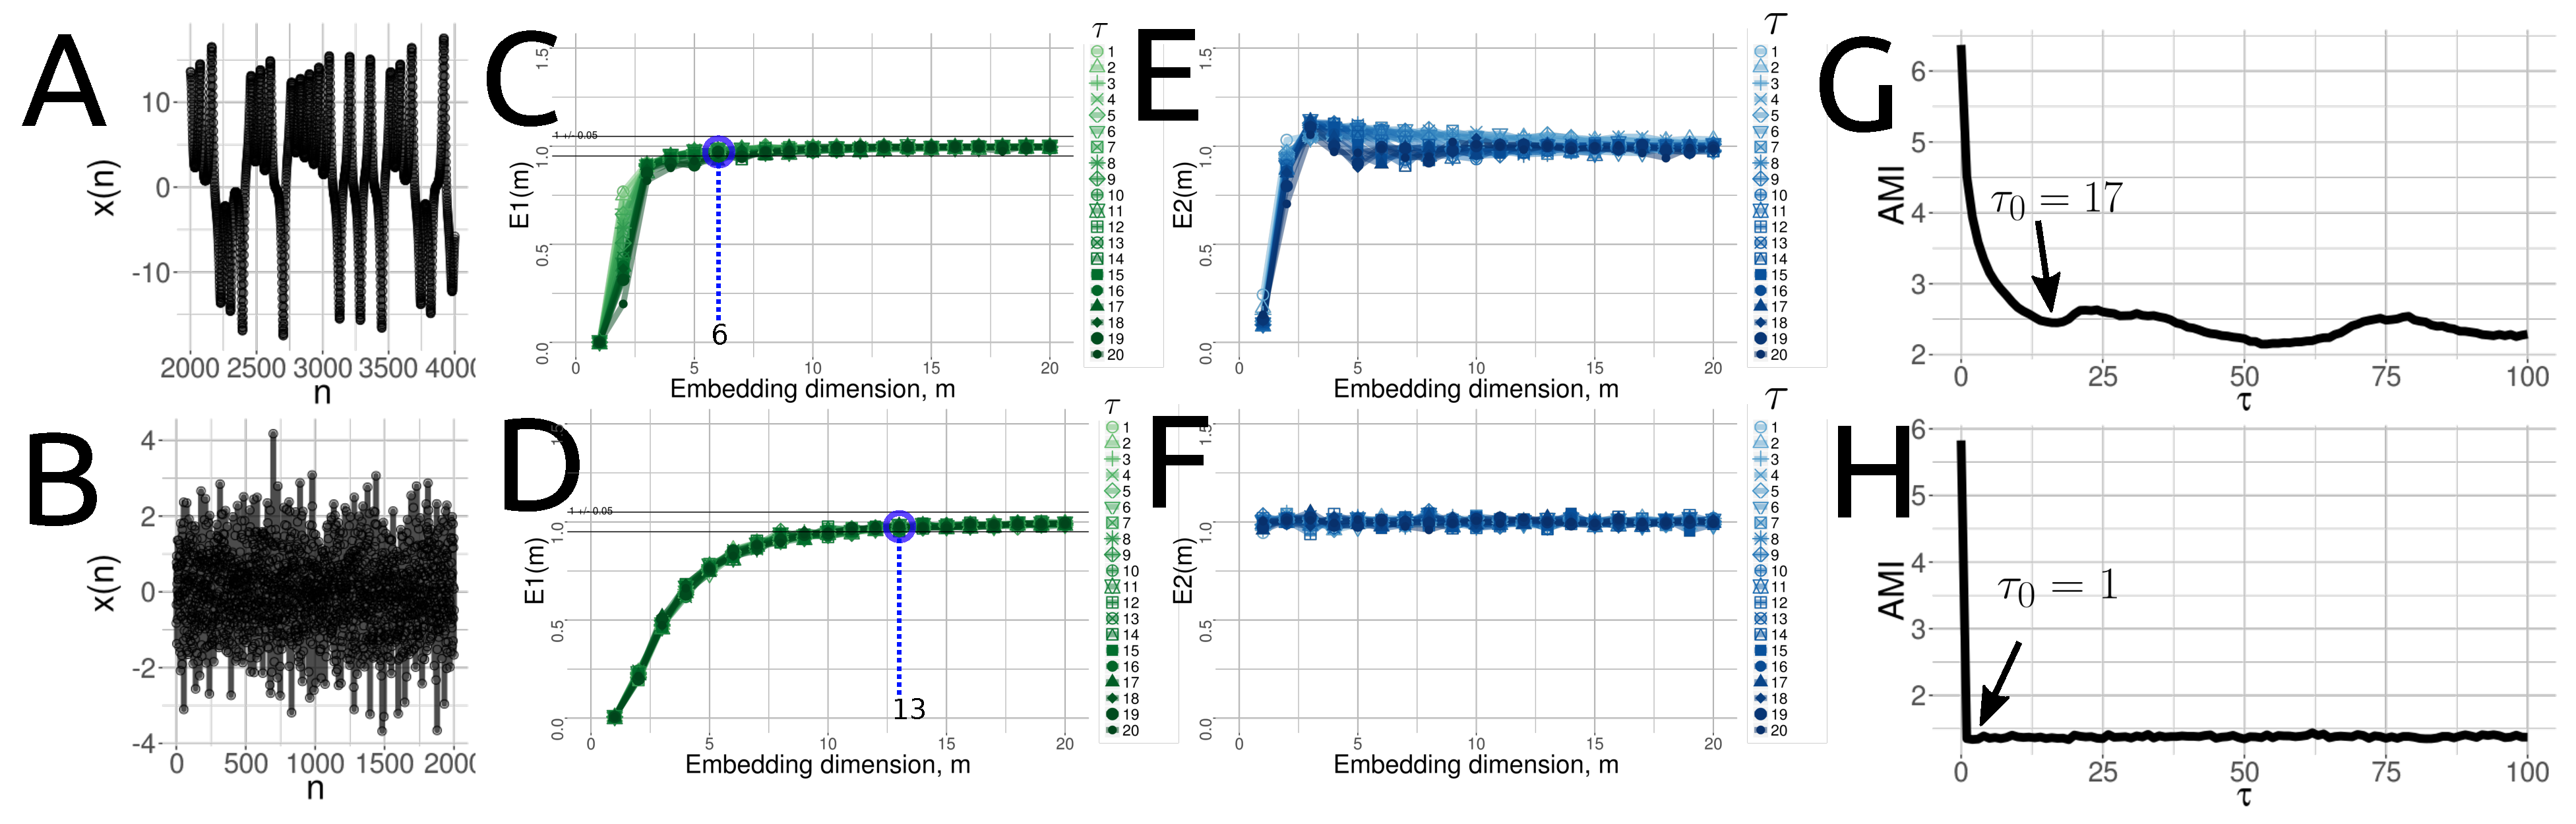
\includegraphics[width=1.0\textwidth]{fig-caoami.pdf}
    \caption{
	{\bf Minimum delay embedding values with AMI's method and minimum dimension embedding values with Cao's method.} 
	(A) chaotic and (B) random time series.
	(C, D) $E_1 (m)$ values and (E, F) $E_2(m)$ values 
	with variations of $\tau$ values from one to twenty
	for chaotic and random time series.
	(G, H) AMI values where its first minimum value in the curve
	is the minimum time delay embedding ($\tau_0$).
	Code and data to reproduce the figure is available in \cite{srep2020}.
        }
    \label{fig:caoami}
\end{figure}
%%---------------------------------(FIGURE)-------------------------------------


%*******************************************************************************
\section*{Recurrence Quantification}\label{sec:recurrence-quantification}
\subsection*{Recurrence Plots}
Originally, Henri Poincar\'e in 1890 introduced the concept of recurrences 
in conservative systems, however such discovery was not put into practice 
until the development of faster computers \cite{marwan2007},
for which Eckmann et al. \cite{eckmann1987} in 1987 introduced a method
where recurrences in the dynamics of a system can be visualised using 
Recurrence Plots. The intention of Eckmann et al. \cite{eckmann1987} was to 
propose a tool, called Recurrence Plot (RP), that provides insights into 
high-dimensional dynamical systems where trajectories are very difficult to 
visualise. Therefore, "RP helps us to investigate the 
$m-$dimensional phase space trajectories through a two-dimensional 
representation of its recurrences" \cite{marwan2015}.
Similarly, Marwan et al. \cite{marwan2015} pointed out that additionally 
to the methodologies of the state space reconstruction and other dynamic 
invariants such as Lyapunov exponent, Kolmogorov-Sinai entropy, 
the recurrences of the trajectories in the phase space can provide 
important clues to characterise natural process that present, for
instance, periodicities (as Milankovitch cycles) or irregular cycles 
(as El Ni\~no Southern Oscillation). 
Such recurrences can not only be presented visually using Recurrence Plots (RP) 
but also be quantified with Recurrence Quantification metrics, which leads 
to applications of these in various areas such as economy, physiology, 
neuroscience, earth science, astrophysics and engineering \cite{marwan2007}.

For the creation of a recurrence plot based on time series 
$\{ \boldsymbol{x}_n \}$, it is first computed the state space 
reconstruction with uniform time-delay embedding 
$X(i)=\{ \boldsymbol{ \tilde{x} }_n, \dots,  
\boldsymbol{ \tilde{x} }_{n -(m-1)\tau} \}$
where $i=1,\dots,N$, $N$ is the number of considered states of $X(i)$ 
and $X(i) \in \mathbb{R}^m$ \cite{eckmann1987}.
The recurrence plot is therefore a two-dimensional $N \times N$ square 
matrix, $\mathbf{R}$, where a black dot is placed at $(i,j)$ 
whenever $X(i)$ is sufficiently close to $X(j)$: 
%%********************************[EQUATION]************************************
\begin{equation}
\mathbf{R}^{m}_{i,j} (\epsilon) = \Theta ( \epsilon_i - || X(i) - X(j) ||
\end{equation}
%%********************************[EQUATION]************************************
where $\quad i,j=1,\dots,N$, $\epsilon$ is a threshold distance, 
$|| \cdotp ||$ a norm, and $\Theta(\cdotp)$ is the Heaviside 
function (i.e. $\Theta(x)=0$, if $x<0$, and $\Theta(x)=1$ otherwise) 
(Fig~\ref{fig:rps}(A,B)) \cite{eckmann1987, marwan2007,marwan2015}.
RP is also characterised with a line of identity (LOI) which is a  
diagonal line due to $ R_{i,j}=1 (i,j=1,\dots,N)$. 


%*******************************************************************************
%*******************************************************************************
%*******************************************************************************
\subsection*{Structures of Recurrence Plots}
Pattern formations in the RPs can be designated either 
as topology for large-scale patterns or texture for small-scale patterns.
In the case of topology, the following pattern formations are commonly presented:
(i) homogeneous where uniform recurrence points are spread in the RP e.g., 
uniformly distributed noise (Fig~\ref{fig:rps}C), 
(ii) periodic and quasi-periodic systems where diagonal lines and 
checkerboard structures represent oscillating systems, e.g., sinusoidal 
signals (Fig~\ref{fig:rps}D), 
(iii) drift where paling or darkening recurrence points away from 
the LOI is caused by drifting systems, 
e.g., logistic map (Fig~\ref{fig:rps}E), and
(iv) disrupted where recurrence points are presented white areas or 
bands that indicate abrupt changes in the dynamics, e.g. Brownian motion 
(Fig~\ref{fig:rps}F) \cite{eckmann1987, marwan2015}.
Texture patterns in RPs can be categorised as:
(i) single or isolated recurrence points that represent rare occurring states, 
and do not persist for any time or fluctuate heavily,
(ii) dots forming diagonal lines where the length of the small-scale parallel 
lines in the diagonal are related to the ratio of determinism or predictability 
in the dynamics of the system, and
(iii) dots forming vertical and horizontal lines where the length of the 
lines represent a time length where a state does not change or change very 
slowly and these patterns formation represent discontinuities in the signal, 
and (iv) dots clustering to inscribe rectangular regions which are related 
to laminar states or singularities \cite{marwan2015}.

Although, each of the previous pattern descriptions of the structures in the 
RP offer an idea of the characteristics of dynamical systems, 
these might be misinterpreted and conclusions might tend to be subjective 
as these require the interpretation of a particular researcher(s).
Because of that, recurrence quantification analyis (RQA) offer objective 
methodologies to quantify such visual characteristics of previous 
recurrent pattern structures in the RP \cite{zbilut1992}.

%---------------------------------(FIGURE)-------------------------------------
\begin{figure}[ht]
\centering
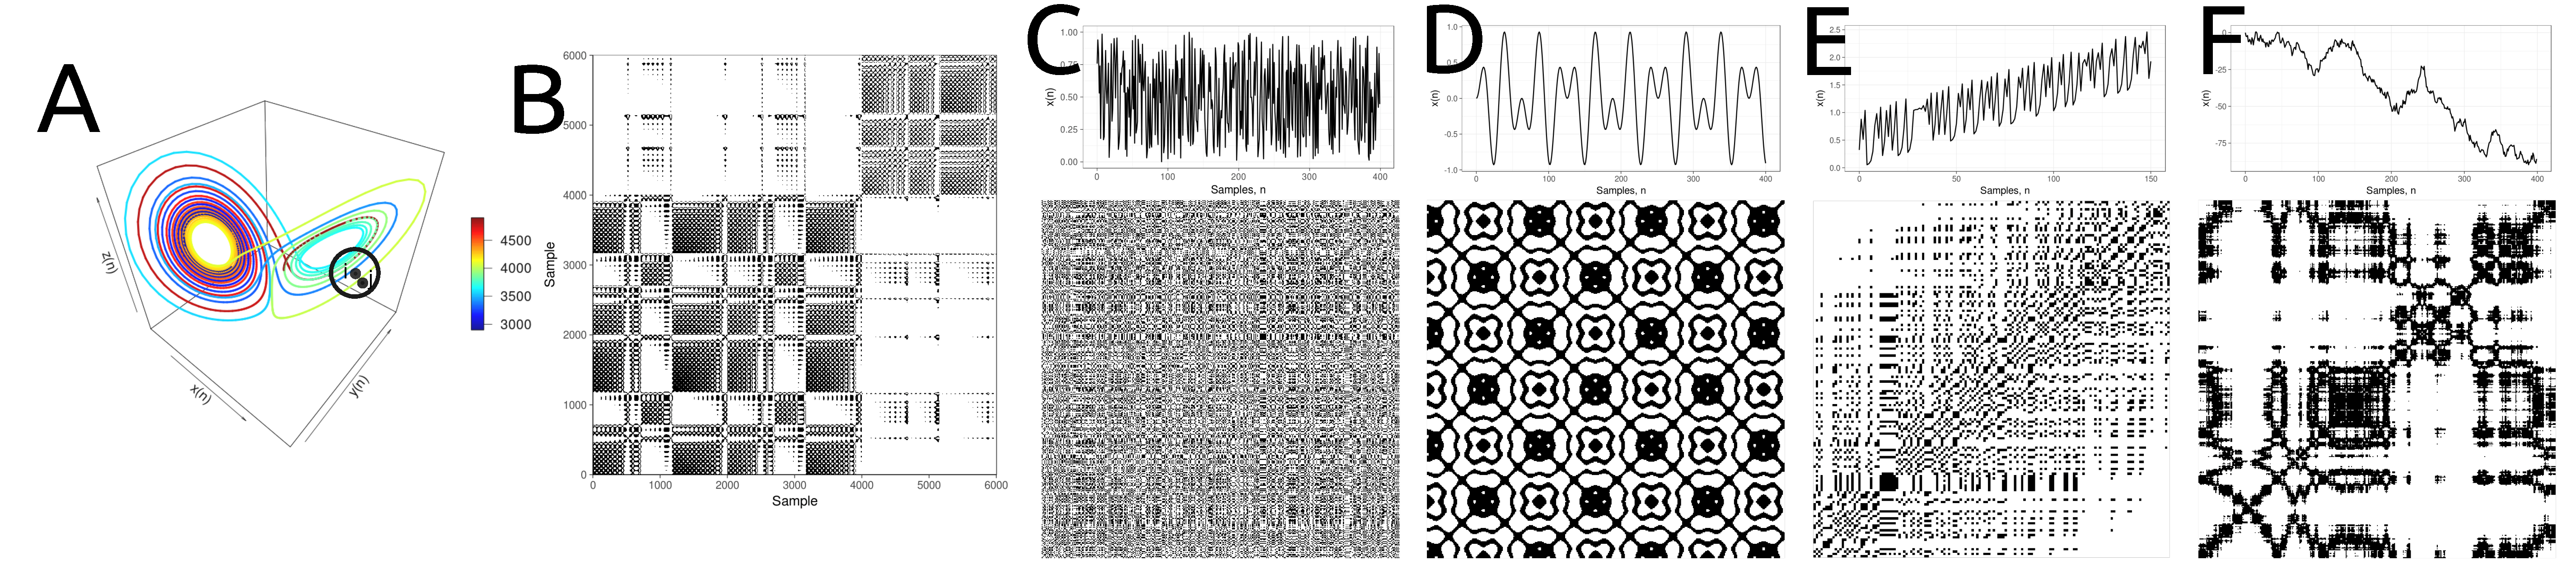
\includegraphics[width=1.0\textwidth]{fig-rps.pdf}
    \caption{
	{\bf Recurrence Plots and its patterns.} 
	(A) State space of the Lorenz system with controlling parameters 
	($\rho=28, \sigma=10, \beta=8/3$) where the point, $j$, in trajectory $X()$ which falls into the neighborhood 
	(black circle) of a given point at $i$ is a recurrent point and is 
	represented as a black dot in the recurrence plot at location 
	$(i, j)$ or white otherwise.
	(B) Recurrence plot using the 
	three components of the Lorenz system and the RP with no embeddings 
	and threshold $\epsilon=5$.
	Time-series with its respective recurrence plot for:
	(C) uniformly distributed noise,
	(D) super-positionet harmonic oscillation 
	($sin( \frac{1}{5}*t) * sin( \frac{5}{100}*t) $),
	(E) drift logistic map ($x_{i+1} = 4 x_i (1- x_i) $) corrupted 
	with a linearly increase term ($0.01*i$), and
	(F) disrupted brownian motion  ($x_{i+1} = x_i + 2*rnorm(1) $).
	This figure is adapted from \cite{marwan2015}.
	Code and data to reproduce the figure is available in \cite{srep2020}.
	}
    \label{fig:rps}
\end{figure}
%%---------------------------------(FIGURE)-------------------------------------



%*******************************************************************************
\subsection*{Recurrence Quantifications Analysis (RQA)}
Originally, Zbilut et al. \cite{zbilut1992} proposed metrics to investigate 
the density of recurrence points in RPs, then histograms of lengths for 
diagonal lines in RPs were studied by \cite{trulla1996} which were the 
introduction to the term recurrence quantification analysis (RQA) 
\cite{marwan2008}. RQA has been applied in many fields such as life science, 
engineering, physics, and others \cite{marwan2008}. Particularly in human 
movement to investigate noise and complexity of postural control 
\cite{rhea2011}, postural control \cite{apthorp2014} or interpersonal 
coordination \cite{duran2017}. The success of RQA is not only due to its 
simple algorithmic implementation but also to its capacity to detect tiny 
modulations in frequency or phase which are not detectable using standard 
methods e.g. spectral or wavelet analysis \cite{marwan2011}, and that 
RQA's metrics are quantitatively and qualitatively independe]nt of embedding 
dimension which is verified experimentally by \cite{iwanski1998}.
RQA metrics comprehend percentage of recurrence, percentage of determinism, 
ratio, Shannon entropy of the frequency distributions of the line lengths,
maximal line length and divergence, trend and laminariy 
\cite{marwan2007, marwan2015}. For this work, we considered only four 
RQA metrics, due to its consistency with our preliminary experiments, 
which are described below. Such metrics are computed the nonlinearTseries 
R package \cite{nonlinearTseries2016}.

\subsubsection*{REC values}
The percentage of recurrence (REC) is defined as
%%********************************[EQUATION]************************************
\begin{equation}
REC(\epsilon,N) = 
		\frac{1}{N^2 - N} \sum^{N}_{i \neq j = 1} 
		\mathbf{R}^{m}_{i,j}(\epsilon),
\end{equation}
%%********************************[EQUATION]************************************
which enumerates the black dots in the RP excluding the line of identity.
REC is a measure of the relative density of recurrence points in the sparse 
matrix \cite{marwan2015}.
%REC is computed as follow with the nonlinearTseries package 
% \cite{nonlinearTseries} 
%  hist = getHistograms(neighs, ntakens, lmin, vmin)
%  # calculate the number of recurrence points from the recurrence rate. The
%  # recurrence rate counts the number of points at every distance in a concrete
%  # side of the main diagonal.
%  # Thus, sum all points for all distances, multiply by 2 (count both sides) and
%  # add the maindiagonal
%  numberRecurrencePoints = sum(hist$recurrenceHist) + ntakens
%  # calculate the recurrence rate dividing the number of recurrent points at a
%  # given distance by all points that could be at that distance
%  recurrence_rate_vector = 
%  hist$recurrenceHist[1:(ntakens - 1)] / ((ntakens - 1):1)
%  # percentage of recurrent points
%  REC = (numberRecurrencePoints) / ntakens ^ 2

\subsubsection*{DET values} 
The percent determinism (DET) is defined as the fraction of recurrence points
that form diagonal lines and it is determined by
%%********************************[EQUATION]************************************
\begin{equation}
DET=
	\frac{\sum^{N}_{l=d_{min}} l H_D{l} }
	     {\sum^{N}_{i,j=1} \mathbf{R}_{i,j}(\epsilon) },
\end{equation}
%%********************************[EQUATION]************************************
where 
%%********************************[EQUATION]************************************
\begin{equation}
H_D(l) = 
	\sum^{N}_{i,j=1} 
	(1- \mathbf{R}_{i-1,j-1}(\epsilon) ) 
	(1- \mathbf{R}_{i+l,j+l}(\epsilon) ) 
	\prod^{l-1}_{k=0}  \mathbf{R}_{i+k,j+k}(\epsilon)
\end{equation}
%%********************************[EQUATION]************************************
is the histogram of the lengths of the diagonal structures in the RP.
DET can be interpreted as the predictability of the system for periodic signals 
which, in essence, have longer diagonal lines than the short diagonals lines
for chaotic signals or absent diagonal lines for stochastic signals 
\cite{marwan2007, marwan2015}. Similarly, DET is considered as a measurement for 
the organisation of points in RPs  \cite{iwanski1998}. 
%percent determinism (DET) is computed as follow with the nonlinearTseries 
%package \cite{nonlinearTseries}  
% calculateDiagonalParameters = function(ntakens, numberRecurrencePoints,
%                                       lmin = 2, lDiagonalHistogram,
%                                       recurrence_rate_vector, maxDistanceMD) {
%  #begin parameter computations
%  num = sum((lmin:ntakens) * lDiagonalHistogram[lmin:ntakens])
%  DET = num / numberRecurrencePoints


\subsubsection*{RATIO values}
RATIO is defined as the ratio between DET and REC and it is calculated from 
the frequency distributions of the lengths of the diagonal lines.
RATIO is useful to discover dynamic transitions \cite{marwan2015}.
%  diagP = calculateDiagonalParameters(
%    ntakens, numberRecurrencePoints, lmin, hist$diagonalHist,
%    recurrence_rate_vector, maxDistanceMD
%  )
% calculateDiagonalParameters = function(ntakens, numberRecurrencePoints,
%                                       lmin = 2, lDiagonalHistogram,
%                                       recurrence_rate_vector, maxDistanceMD) {
%  #begin parameter computations
%  num = sum((lmin:ntakens) * lDiagonalHistogram[lmin:ntakens])
%  DET = num / numberRecurrencePoints
% 
%
%    RATIO = diagP$DET / REC
%

\subsubsection*{ENT values}
ENT is the Shannon entropy of the frequency distribution of the diagonal 
line lengths and it is defined as
%%********************************[EQUATION]************************************
\begin{equation}
ENT= - \sum^{N}_{l=d_{min}} p(l) ln p(l) \quad with 
	\quad p(l)=\frac{ H_D(l) }{ \sum^{N}_{ l=d_{min} } H_D(l) }.
\end{equation}
%%********************************[EQUATION]************************************
ENT reflects the complexity of the deterministic structure in the system.
For instance, for uncorrelated noise or oscillations, 
the value of ENT is rather small and indicates low complexity of the system,
therefore "the higher the ENT is the more complex the dynamics are" 
\cite{marwan2007, marwan2015}.
%#'  \item \emph{ENTR}: Shannon entropy of the diagonal line lengths distribution
%
%calculateDiagonalParameters = function(ntakens, numberRecurrencePoints,
%                                       lmin = 2, lDiagonalHistogram,
%                                       recurrence_rate_vector, maxDistanceMD) {
%
%  pl = lDiagonalHistogram / sum(lDiagonalHistogram)
%  diff_0 = which(pl > 0)
%  ENTR = -sum(pl[diff_0] * log(pl[diff_0]))

 
\subsection*{Sensitivity and robustness of RPs and RQA.}
RP and RQA are a very young field in nonlinear dynamics and many questions 
are still open, for instance, different parameters for window length size 
of the time series, embedding parameters or recurrence threshold can 
generate different results in RQA's metrics \cite{marwan2011, eckmann1987}.

The selection of recurrence threshold, $\epsilon$, can depend on the system 
that is analysed. For instance, when studying dynamical invariants $\epsilon$ 
require to be very small, for trajectory reconstruction $\epsilon$ requires 
to have a large thresholds or when studying dynamical transition 
there is little importance about the selection of the threshold 
\cite{marwan2011}. Other criteria for the selection of $\epsilon$ is that 
the recurrence threshold  should be five times larger 
than the standard deviation of the observational noise
or the use of diagonal structures within the RP is suggested in order
to find the optimal recurrence threshold for (quasi-)periodic process 
\cite{marwan2011}.
Similarly, Iwanski et al. \cite{iwanski1998} highlighted the importance 
of choosing the right embedding parameters to perform RQA for which 
many experiments have to be performed using different parameters in order 
to have a better intuition of the nature of the time series and how 
this is represented by using RQA.

With that in mind, this work explores the sensitivity and robustness 
of the window size of time series, embedding parameters for RSS with UTDE 
and recurrence threshold for RP and RQA in order to gain a better insight 
into the underlying time series collected from inertial sensors in the 
context of human-humanoid imitation activities.
%Such changes of recurrence threshold values 
%can modify the patterns in RPs and therefore the values of RQA metrics.
%We therefore computed 3D surfaces to explore the sensibility and robustness of 
%embedding parameters and recurrence threshold in RQA  metrics. Following the 
%same methodology of computing 3D surfaces, we also considered variation of 
%window length size to present RQA metrics dependencies with embedding 
%parameters, recurrence thresholds and window length size.


%Choosing an appropriate recurrence threshold is crucial so as to get 
%meaningful representations in RP and RQA, however, 

%Iwansky et al. \cite{iwanski1998} stated that patterns in Recurrence Plots and 
%metrics for RQA are independent of embedding dimension parameters, 
%however, that is not the case when using 
%different recurrence thresholds. 


%Zbilut et al. \cite{zbilut1992} established RQA metrics with the aim of 
%determining embedding parameters, their method consisted on creating 3D 
%surfaces with RQA metrics with an increase of embedding parameters 
%($m$ and $\tau$), then Zbilut et al. \cite{zbilut1992} explored 
%fluctuations and gradual changes in the 3D surfaces that provide information 
%about the embeddings. Much recently, Marwan et al. \cite{marwan2015} 
%created 3D surfaces for visual selection of not only embedding parameters 
%but also recurrence thresholds. Following same methodologies, we explored 
%the stability and robustness of RQA metrics (REC, DET, RATIO and ENTR)
%using 3D surfaces by an unitary increase of the pair embedding 
%parameters ($0 \ge m \le 10$, $0 \ge \tau \le 10$) and a decimal increase 
%of 0.1 for recurrence thresholds ($ 0.2 \ge \epsilon \le 3 $) 
%(Fig.~\ref{fig:topo_rqas}).



%*******************************************************************************
%*******************************************************************************
%*******************************************************************************
\section*{Experiment} \label{sec:experiment}
We conducted an experiment in the context of human-humanoid imitation (HHI) 
activities where participants were asked to imitate simple horizontal and 
vertical arm movements performed by NAO, a humanoid robot \cite{gouaillier2009}.
Such simple movements were repeated ten times for the participant 
who copied NAO's arm movements in a face-to-face imitation activity.
Also, wearable inertial measurement unit (IMU) sensors were attached 
to the right hand of the participant and to the left hand of the robot 
(Figure~\ref{fig:hri} A,C). Data were then collected with four NeMEMSi 
IMU sensors with sampling rate of 50Hz provinding tri-axial data of the 
accelerometer, gyroscope and magnetometer sensors and quaternions 
\cite{Comotti2014}.
%%---------------------------------(FIGURE)-------------------------------------
\begin{figure}[ht]
  \centering
\includegraphics[width=1.0\textwidth]{fig-hri}
    \caption{
	{\bf Human-humanoid imitation activities.} 
    		Face-to-face human-humanoid imitation (HHI) activities for 
		(A) HHI of horizontal arm movement, 
		(B) Humanoid horizontal arm movement,
		(C) HHI of vertical arm movement, and 
		(D) Humanoid vertical arm movement.
        }
    \label{fig:hri}
\end{figure}
%%---------------------------------(FIGURE)------------------------------------

\subsection*{Participants}
Twenty-three participants,
from now on defined as $pN$ where $N$ is the number of participant, were 
invited to do the experiment. However, data for three participants were 
not used because the instructions for $p01$, who was the only left-handed,
were mistakenly given in a way that movements were performed different
from what had been planned, and for participants $p13$ and $p16$ 
data were corrupted because of problems with Bluetooth communications with sensors. 
With that in mind, data for twenty participants were analysed in this work.
Of the twenty participants, all of them are right-handed healthy participants 
of whom four are females and sixteen are males with a mean and standard 
deviation (SD) age of mean=19.8 (SD=1.39). 

\subsection*{Ethics}
All participants provided informed consent forms prior to participation 
in the experiment. Hence, the experiments were conducted in November 2016 and 
participants confirmed reading and understanding the participant information sheet of the 
experiments and were able to withdraw from the experiment at any time without giving
any reason. The design of the experiments adhered to the University of Birmingham
regulations, data were anonymised and videos were stored only on a 
personal computer in accordance with the Data Protection Act 1998. 
%Refer to Appendix D for further information about the ethics, 
%online participation information sheets and experiment check list.


\subsection*{Human-humanoid imitation activities}
For human-humanoid imitation (HHI) activities four neMEMSi sensors were used,
two of which were attached to the right hand of the participant and the 
other two to the left hand of the humanoid robot.
Then, each participant was asked to imitate repetitions of simple horizontal
and vertical arm movements performed by the humanoid robot in the following 
conditions:
(i) ten repetitions of horizontal arm movement at normal (HN) 
	and faster (HF) speed (Figure~\ref{fig:hri} A), and
(ii) ten repetitions of vertical arm movement at normal (VN) 
	and faster (VF) speed (Figure~\ref{fig:hri} C).
The normal and faster speed of arm movements is defined by the duration 
in number of samples of one repetition of NAO's arm movements. 
We select NAO's arm movements duration to distinguish between normal and 
faster arm movements as NAO's movements have less variation 
for such repetitive movements. 
The duration for one repetition of the horizontal 
arm movement at normal speed, HN, is 5 seconds considering 
that each repetition last around 250 samples.
For horizontal arm movement at faster speed, HF, each repetition were performed 
in 2 seconds which correspond to 90 samples of data.
The vertical arm movement at normal speed, VN, were performed  in 6 seconds 
which is around 300 samples of data. For vertical arm movement at 
faster speed, VF, each repetition lasts about 2.4 seconds which correspond 
to 120 samples of data.
To visualise the distinction between normal and faster speed for horizontal 
and vertical arm movements, Fig~\ref{fig:sts} shows smoothed time series 
for axes Z and Y of the gyroscope sensors with four window lengths: 
2-sec (100-samples), 5-sec (250-samples), 10-sec (500-samples) 
and 15-sec (750-samples).
%%---------------------------------(FIGURE)-------------------------------------
\begin{figure}[ht] 
\centering
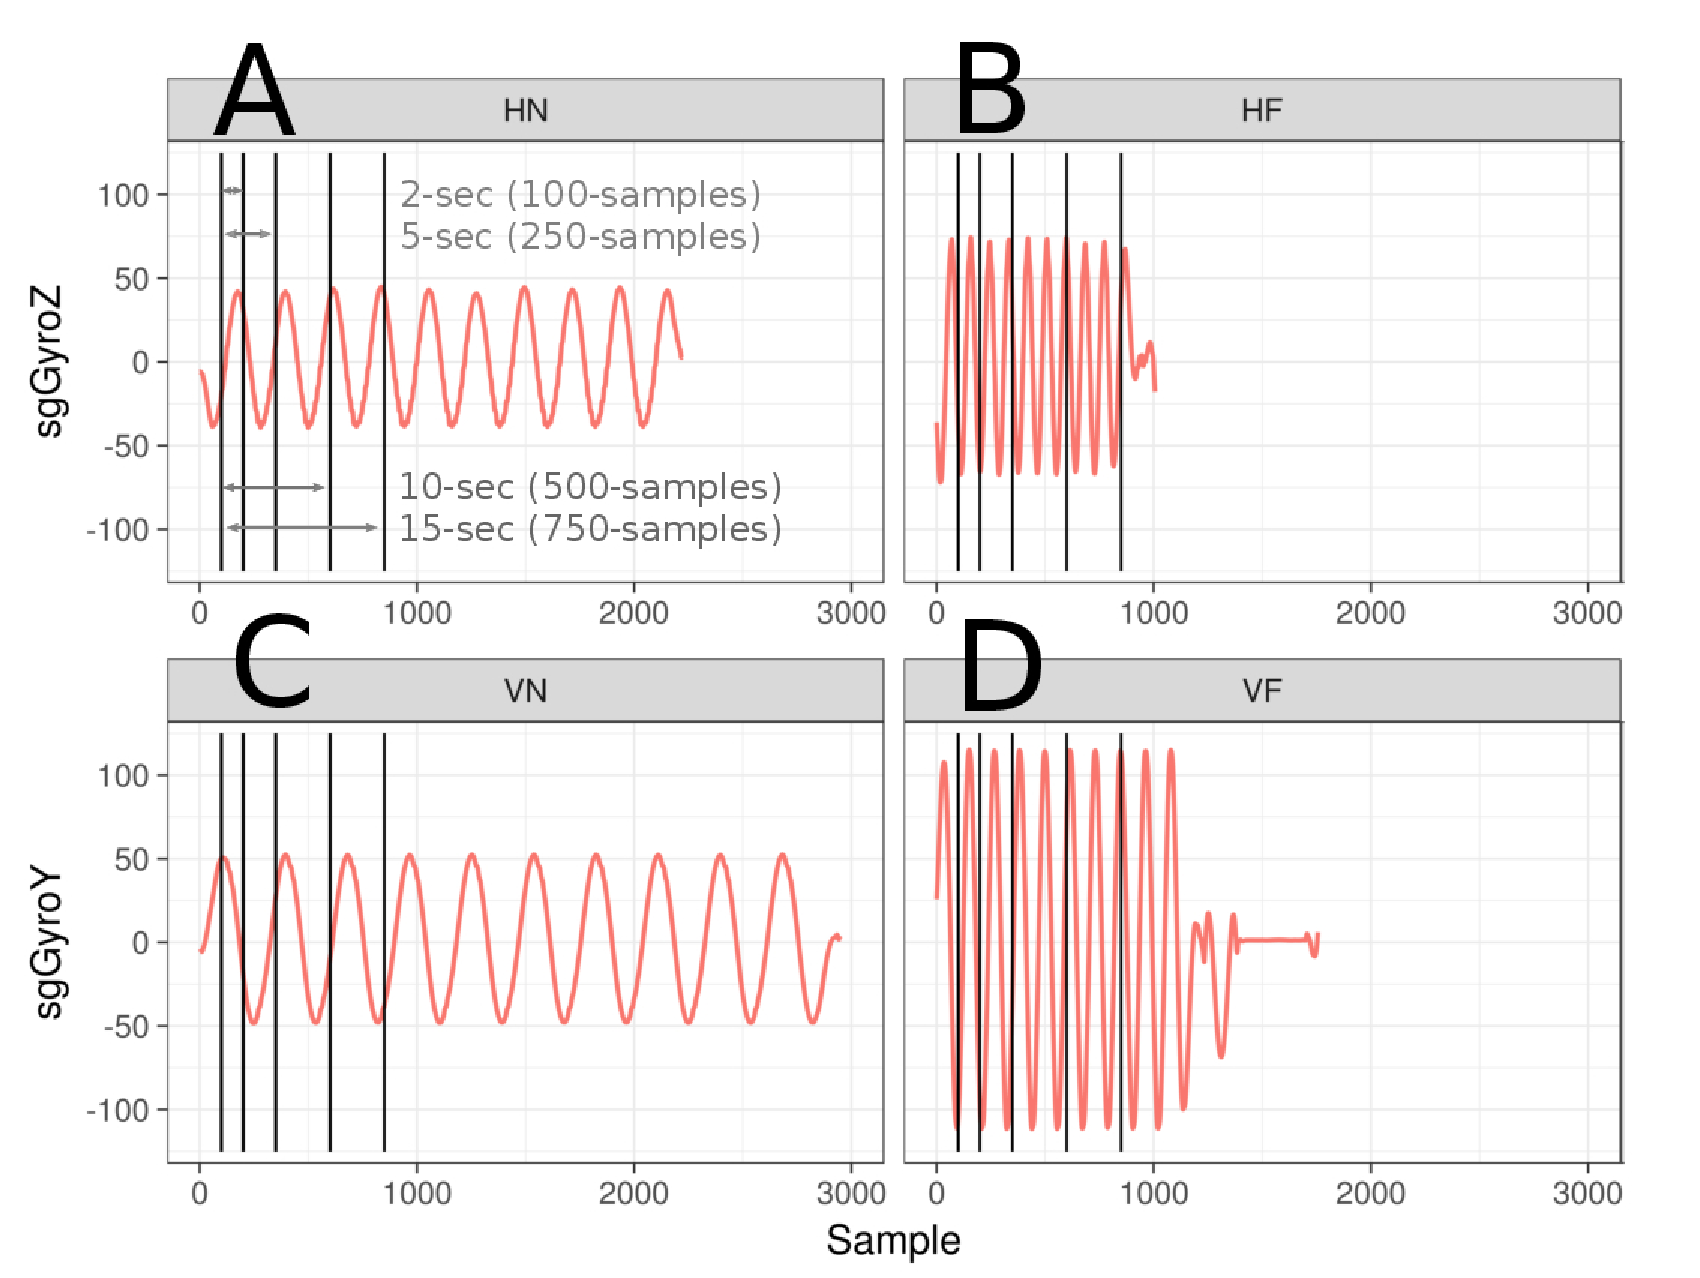
\includegraphics[width=1.0\textwidth]{fig-sts.pdf}
    \caption{
	{\bf Time series duration of horizontal and vertical arm movements.} 
    		Time series of smoothed data from gyroscope sensor 
		for different speed arm movements performed by NAO: 
		(A) Horizontal Normal arm movement (HN), 
		(B) Horizontal Faster arm movement (HF),
		(C) Vertical Normal arm movement (VN) and 
		(D) Vertical Faster arm movement (VF).
		Additionally, 
		(A) shows window sizes for 2-seconds (100 samples), 
		5-seconds (250 samples), 10-seconds (500 samples) 
		and 15-seconds (750 samples)
		which are also presented in (B), (C) and (D).
		Code and data to reproduce the figure is available in \cite{srep2020}.
        }
	\label{fig:sts}
\end{figure}
%%---------------------------------(FIGURE)------------------------------------

\subsection*{Data collection from inertial measurement units} 
\label{sec:experiment:subsec:imu}
To give insight to the research questions, 
we considered various conditions of time series collected for this work: 
\begin{itemize}
\item Three levels of smoothness for normalised data 
	(e.g., sg0zmuv, sg1zmuv and sg2zmuv) where sg 
	stands for Savitzky-Golay filter with two different filter lengths (29 and 159) 
	and the same polynomial degree of 5 using the function \texttt{sgolay(p,n,m)} \cite{Rsignal}
	and zmuv is zero mean unit variance.
\item four arm movement activities with two velocities: 
	horizontal normal (HN), horizontal faster (HF), 
	vertical normal (VN), and vertical faster (VF), and
\item four window lengths: 2-sec (100 samples), 5-sec (250 samples), 
	10-sec (500 samples) and 15-sec (750 samples).
\end{itemize}
%After the data collection, raw time series were windowed, normalised and smoothed. 
Due to space limitations and to have simple visualisation, 
we only present 10-sec (500 samples) window length time series for 
three participants (p01, p01 and p03) performing horizontal 
arm movements (axis GyroZ) and vertical arm movements (axis GyroY) (Figs \ref{fig:ts}).
%%---------------------------------(FIGURE)-------------------------------------
\begin{figure}[ht]
\centering
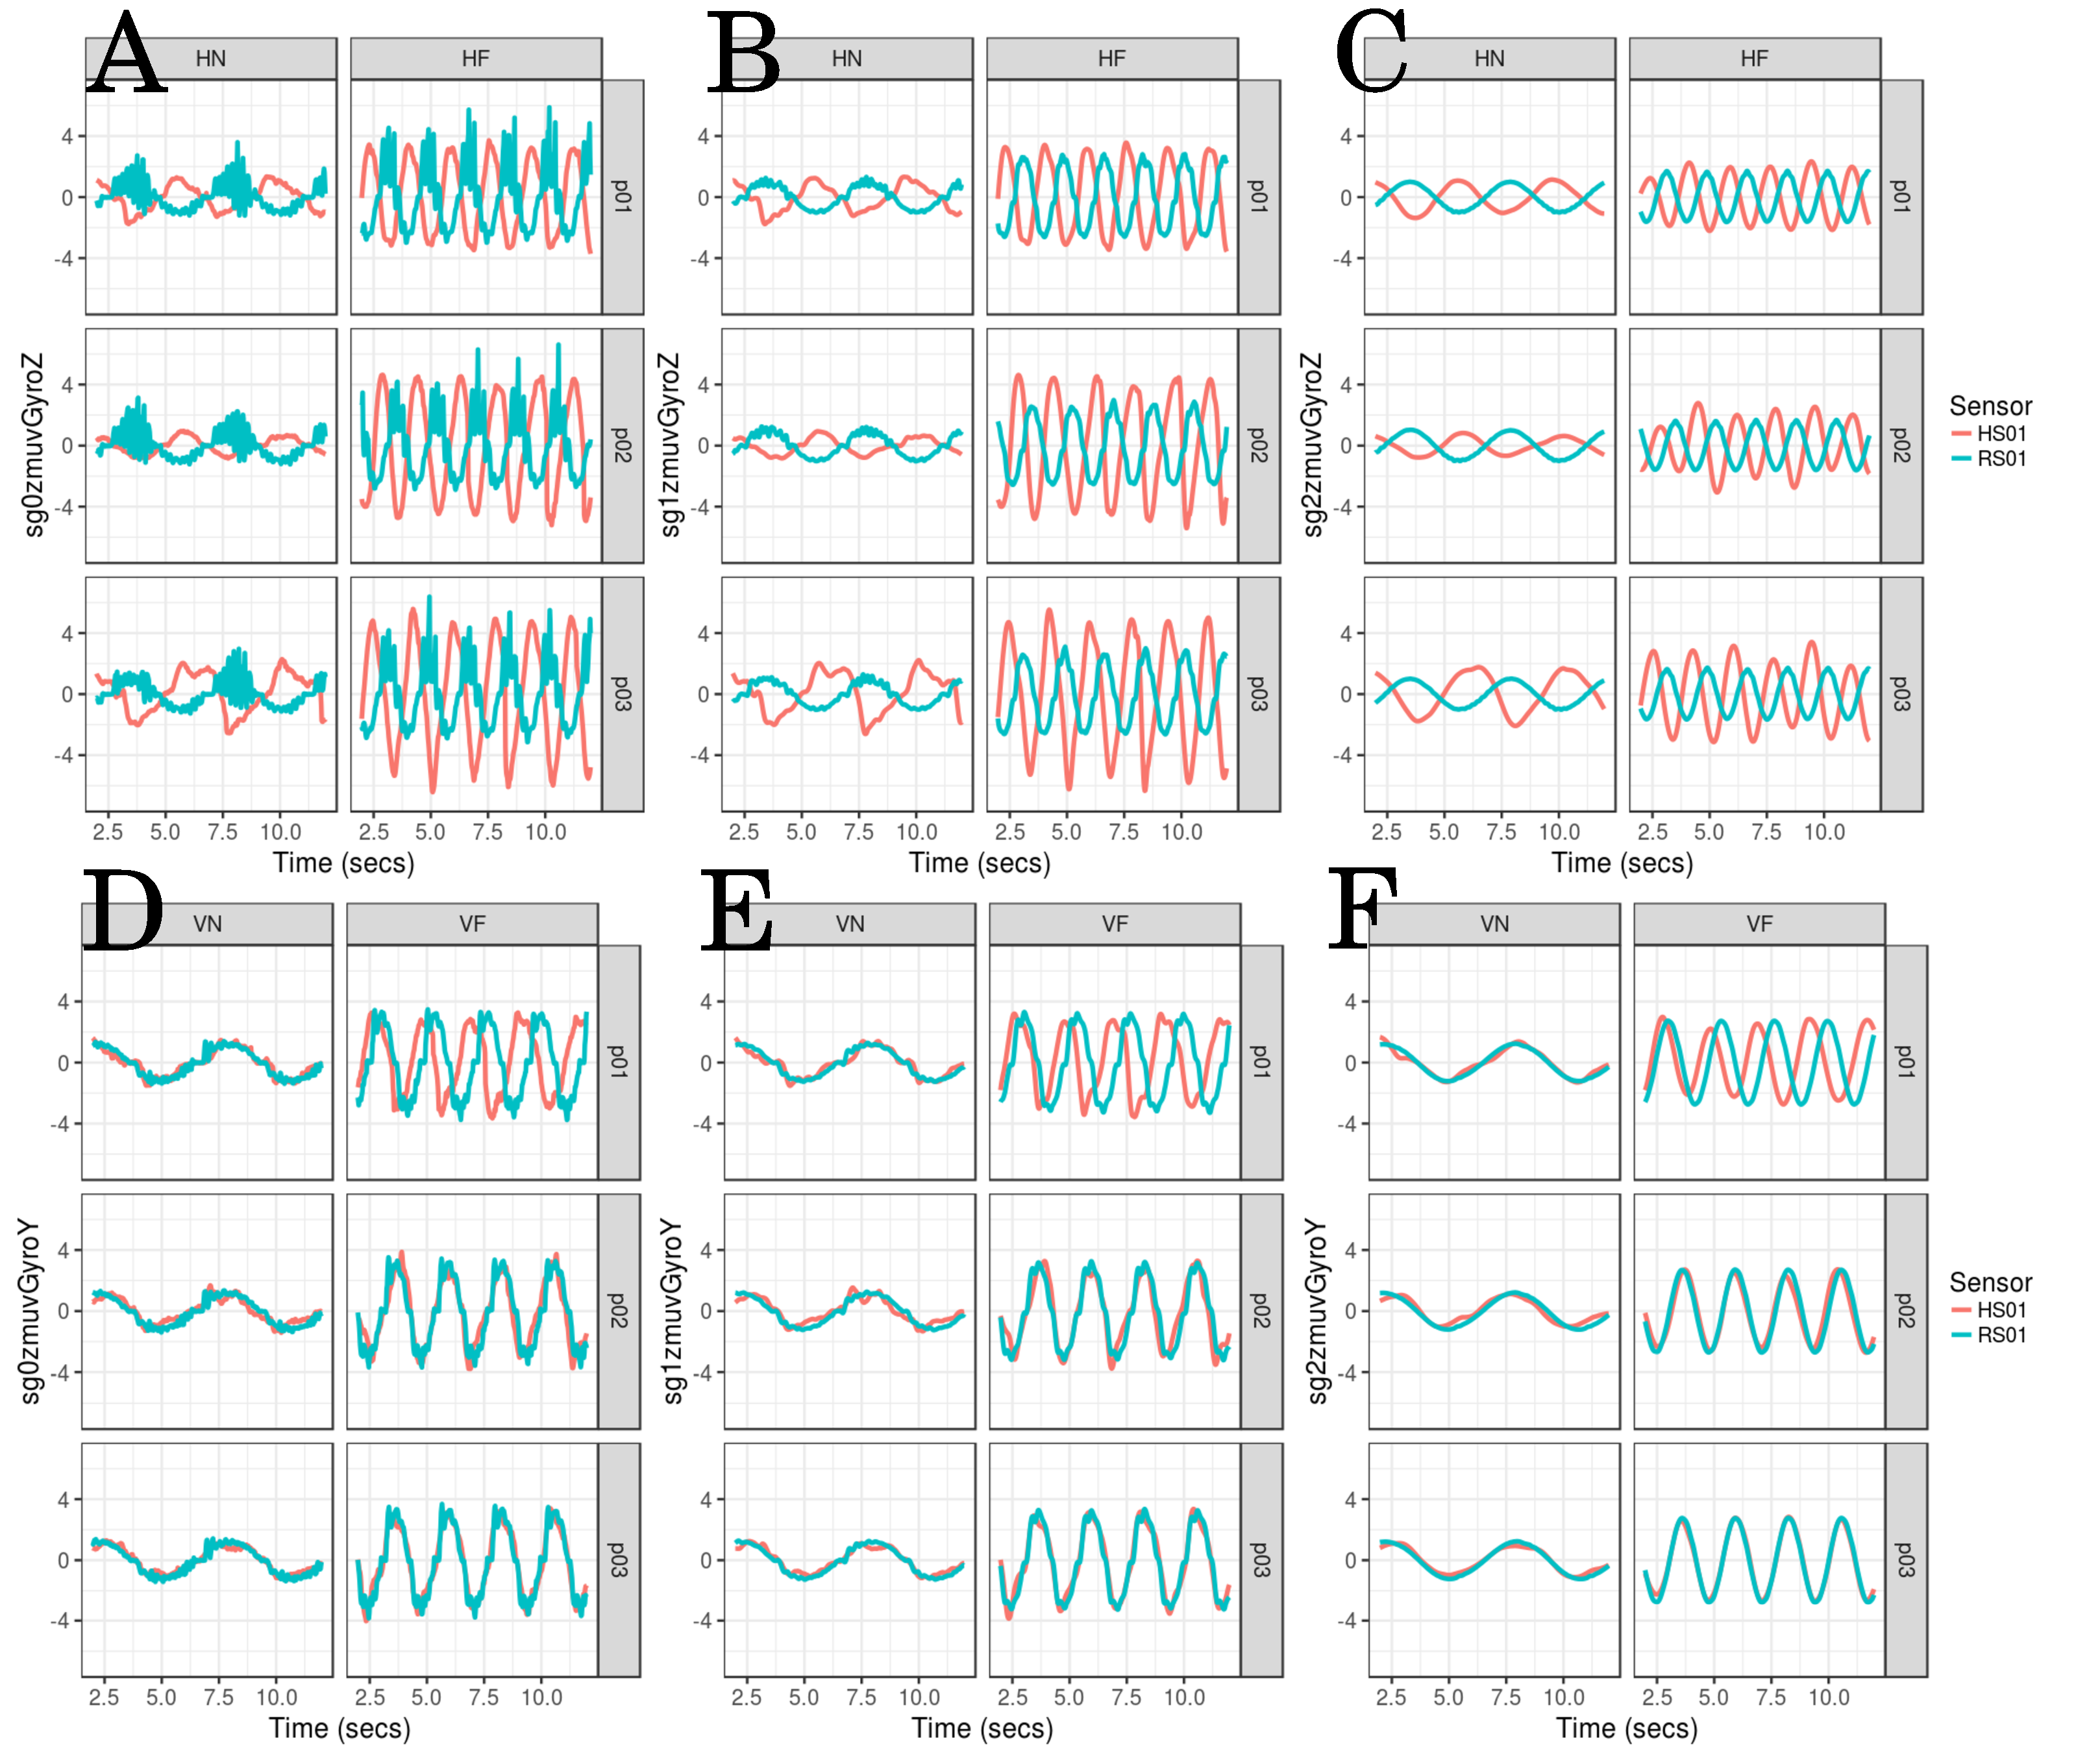
\includegraphics[width=1.0\textwidth]{fig-fig1.pdf}
    	\caption{ 
	{\bf Time series for horizontal and vertical arm movements.}
		(A/D) raw-normalised (sg0zmuv), 
		(B/E) normalised-smoothed 1 (sg1zmuv) and
		(C/F) normalised-smoothed 2 (sg2zmuv).
		Time series are only for three participants 
		($p01$, $p02$, and $p03$) 
		for horizontal and vertical arm movements in normal 
		and faster velocity (HN, HF, VN, VF) 
		with the normalised GyroZ or GyroY axis 
		and with one sensor attached to the participant (HS01) 
		and other sensor attached to the robot (RS01).	
	Code and data to reproduce the figure is available in \cite{srep2020}.
        }
    \label{fig:ts}
\end{figure}
%%---------------------------------(FIGURE)------------------------------------




\subsubsection*{Raw data}
%Considering the work of \cite{shoaib2016} which provided evidence of an 
%improvement in recognition activities when combining data from 
%accelerometer and gyroscope. 
We focus our analysis from data of the 
accelerometer and gyroscope of the NeMEMsi sensors \cite{Comotti2014} and 
leave the data of the magnetometer and quaternions for further investigation 
because of their possible variations with regard to magnetic disturbances \cite{shoaib2016}.
Data from the accelerometer is defined by triaxial time series 
$A_x(n)$, $A_y(n)$, $A_z(n)$ which forms the matrix $\boldsymbol{A}$ 
(Eq.~\ref{eq:AG}), and the same for data from the gyroscope 
which is defined by triaxial time-series of $G_x(n)$, $G_y(n)$, $G_z(n)$ 
representing the matrix $\boldsymbol{G}$ (Eq.~\ref{eq:AG}).
Both triaxial time series of each sensor, $a$ and $g$, are denoted with 
its respective axes subscripts $x,y,z$, where $n$ is the sample index 
and $N$ is the same maximum length of all axes for the time series.
%Matrices  $\boldsymbol{A}$ and $\boldsymbol{G}$ are represented as follows
%%---------------------------------(EQUATION)----------------------------------
\begin{equation}\label{eq:AG}
\boldsymbol{A} =
\begin{pmatrix}
  A_x(n) \\
  A_y(n) \\
  A_z(n)
\end{pmatrix}
=
\begin{pmatrix}
 a_x(1),a_x(2),\dots,a_x(N) \\
 a_y(1),a_y(2),\dots,a_y(N) \\
 a_z(1),a_z(2),\dots,a_z(N) 
\end{pmatrix},
%\end{equation}
%%---------------------------------(EQUATION)-----------------------------------
%and 
%%---------------------------------(EQUATION)-----------------------------------
%\begin{equation}\label{eq:G}
\boldsymbol{G} =
\begin{pmatrix}
 G_x(n) \\
 G_y(n) \\
 G_z(n)
\end{pmatrix}
=
\begin{pmatrix}
 g_x(1),g_x(2),\dots,g_x(N) \\
 g_y(1),g_y(2),\dots,g_y(N) \\
 g_z(1),g_z(2),\dots,g_z(N) 
\end{pmatrix}.
\end{equation}
%%---------------------------------(EQUATION)-----------------------------------


\subsubsection*{Postprocessing data}
After the collection of raw data from four NeMEMsi sensors,
time synchronisation alignment and interpolation were performed 
in order to create time series with the same length and synchronised time.
We refer the reader to \cite{Comotti2014} for further
details about the time synchronisation process.

\subsubsection*{Normalising data}
Data is normalised to be zero mean and unit variance.
The sample mean and sample standard deviation using $x(n)$ is given by
%%---------------------------------(EQUATION)----------------------------------
\begin{equation}\label{eq:ms}
\mu_{x(n)}= \frac{1}{N} ( \sum_{i=1}^N x(i) ), \quad 
	\sigma_{x(n)} =  \sqrt{ \frac{  \sum_{1=1}^N ( x(i) - \mu_{x(n)} )^2 }{ N-1 }  },      
\end{equation}
%%---------------------------------(EQUATION)----------------------------------
and the normalised data, $\hat{x}(n)$, is computed as follows
%%---------------------------------(EQUATION)----------------------------------
\begin{equation}\label{eq:normalization}
\hat{x} (n) = \frac{   x(n) -  \mu_{x(n)}  }{   \sigma_{x(n)} }.   
\end{equation}
%%---------------------------------(EQUATION)----------------------------------

\subsubsection*{Smoothing data}
Commonly, a low-pass filter is use either to capture the low 
frequencies that represent \%99 of the human body energy or to get 
the gravitational and body motion components of 
accelerations \cite{anguita2013}. However, the elimination of 
a range of frequencies is not the main focus of this work but 
the conservation of the structure of time series in terms of 
their width and heights where, for instance, Savitzky-Golay filter 
can be a way to accomplish such task \cite{press1992}. 
Savitzky-Golay filter is based on the 
principle of moving window averaging which preserves the area under 
the curve (the zeroth moment), its mean position in time 
(the first moment) but the line width (the second moment) is violated 
and that results, for example, in the case of spectrometric data, into
a narrow spectral line with reduced height and width. 
With that in mind, the aim of Savitzky-Golay filtering is to find filter 
coefficients $c_n$ that preserve higher momentums which are based on local 
least-square polynomial approximations \cite{savitzkygolay1964, 
press1992, schafer2011}.
Therefore, Savitzky-Golay coefficients are computed with \texttt{sgolay(p,n,m)} 
in R where \texttt{p} is the filter order, 
\texttt{n} is the filter length (must be odd) and \texttt{m} is the 
$m$-th derivative of the filter coefficients \cite{Rsignal}. 
Smoothed signal is represented with a tilde over the original 
variable of the signal: $\tilde{x}(n)$.

\subsubsection*{Windowing data size}
With regards to the window size, Shoaib et al. in 2016 \cite{shoaib2016} 
investigated effects of seven window lengths (2, 5, 10, 15, 20, 25, 30 seconds)
and combination of inertial sensors (accelerometer, gyroscope and linear 
acceleration sensor) to improve the activity recognition performance for 
repetitive activities (walking, jogging and biking) and less repetitive 
activities (smoking, eating, giving a talk or drinking a coffee).
With that in mind, Shoaib et al. \cite{shoaib2016} concluded that the 
increase of window length improve the recognition of complex activities 
because these requires a large window length to learn the repetitive 
motion patterns. Particularly, one of the recommendations is to use large 
window size to recognise less repetitive activities which mainly involve 
random hand gestures. Therefore, for the four activities 
(HN, HF, VN, and VF) in this work, which are mainly repetitive, 
we select only four window sizes for analysis: 2-s window (100 samples), 
5-s window (250 samples), 10-s (500 samples) and 15-s window (750 samples) 
(Fig~\ref{fig:sts}).

%*******************************************************************************
%*******************************************************************************
%*******************************************************************************
\section*{Results}

\subsection*{Reconstructed State Spaces}
As noted in the Introduction, a challenge in the implementation of uniform time-delay embedding 
arises from the selection of embedding parameters because of the uniqueness of each time series 
in terms of its structure (e.g., modulation of amplitude, frequency, phase etc.). 
With that in mind, the options are to either calculate embedding parameters for each unique 
instance (which can make comparison challenging) or to find parameters which can apply to all 
instances in the study.
We recognise that the latter approach is not without its problems, 
but our approach is to compute sample mean over all values in each of the conditions of the 
time series for minimum dimension and minimum delay values.

\subsubsection*{Minimum embedding parameters}
Minimum embedding parameters were initially computed using False Nearest Neighbour (FNN) 
and Average Mutual Information (AMI).   We used FNN to calculate a value for $m$
to unfold the attractors and AMI to calculate a value for $\tau$ and maxime the 
information in the unfolded attractor.
To illustrate this, figure \ref{fig:cao_ami} (A) show box plots for minimum embedding 
values for sensors on the wrist of the human (HS01) and the robot (RS01).   
As we had assumed, minimum embedding values for HS01 show greater variation than 
those for RS01 (as indicated by differences in interquartile ranges).  
Additionally, figure \ref{fig:cao_ami} (A) show a decrease in mean values (rhombus) in the box plots 
as smoothness of the time-series increases (see sg0, sg1, sg2).  
Figure \ref{fig:cao_ami} (B) show box plots for Average Mutual Information (AMI).  
One can see that, in contrast to RS01, minimum values for HS01 tend to spread 
as the smoothness of the time-series increases.
The sample mean for minimum value of embedding parameter, 
$m$ derived from FNN  (figures \ref{fig:cao_ami} A) is $\overline{m}_0=6$ 
and $\tau$ from AMI (figures \ref{fig:cao_ami} B) is $\overline{\tau}_0=8$.

%---------------------------------(FIGURE)-------------------------------------
\begin{figure}[ht]
\centering
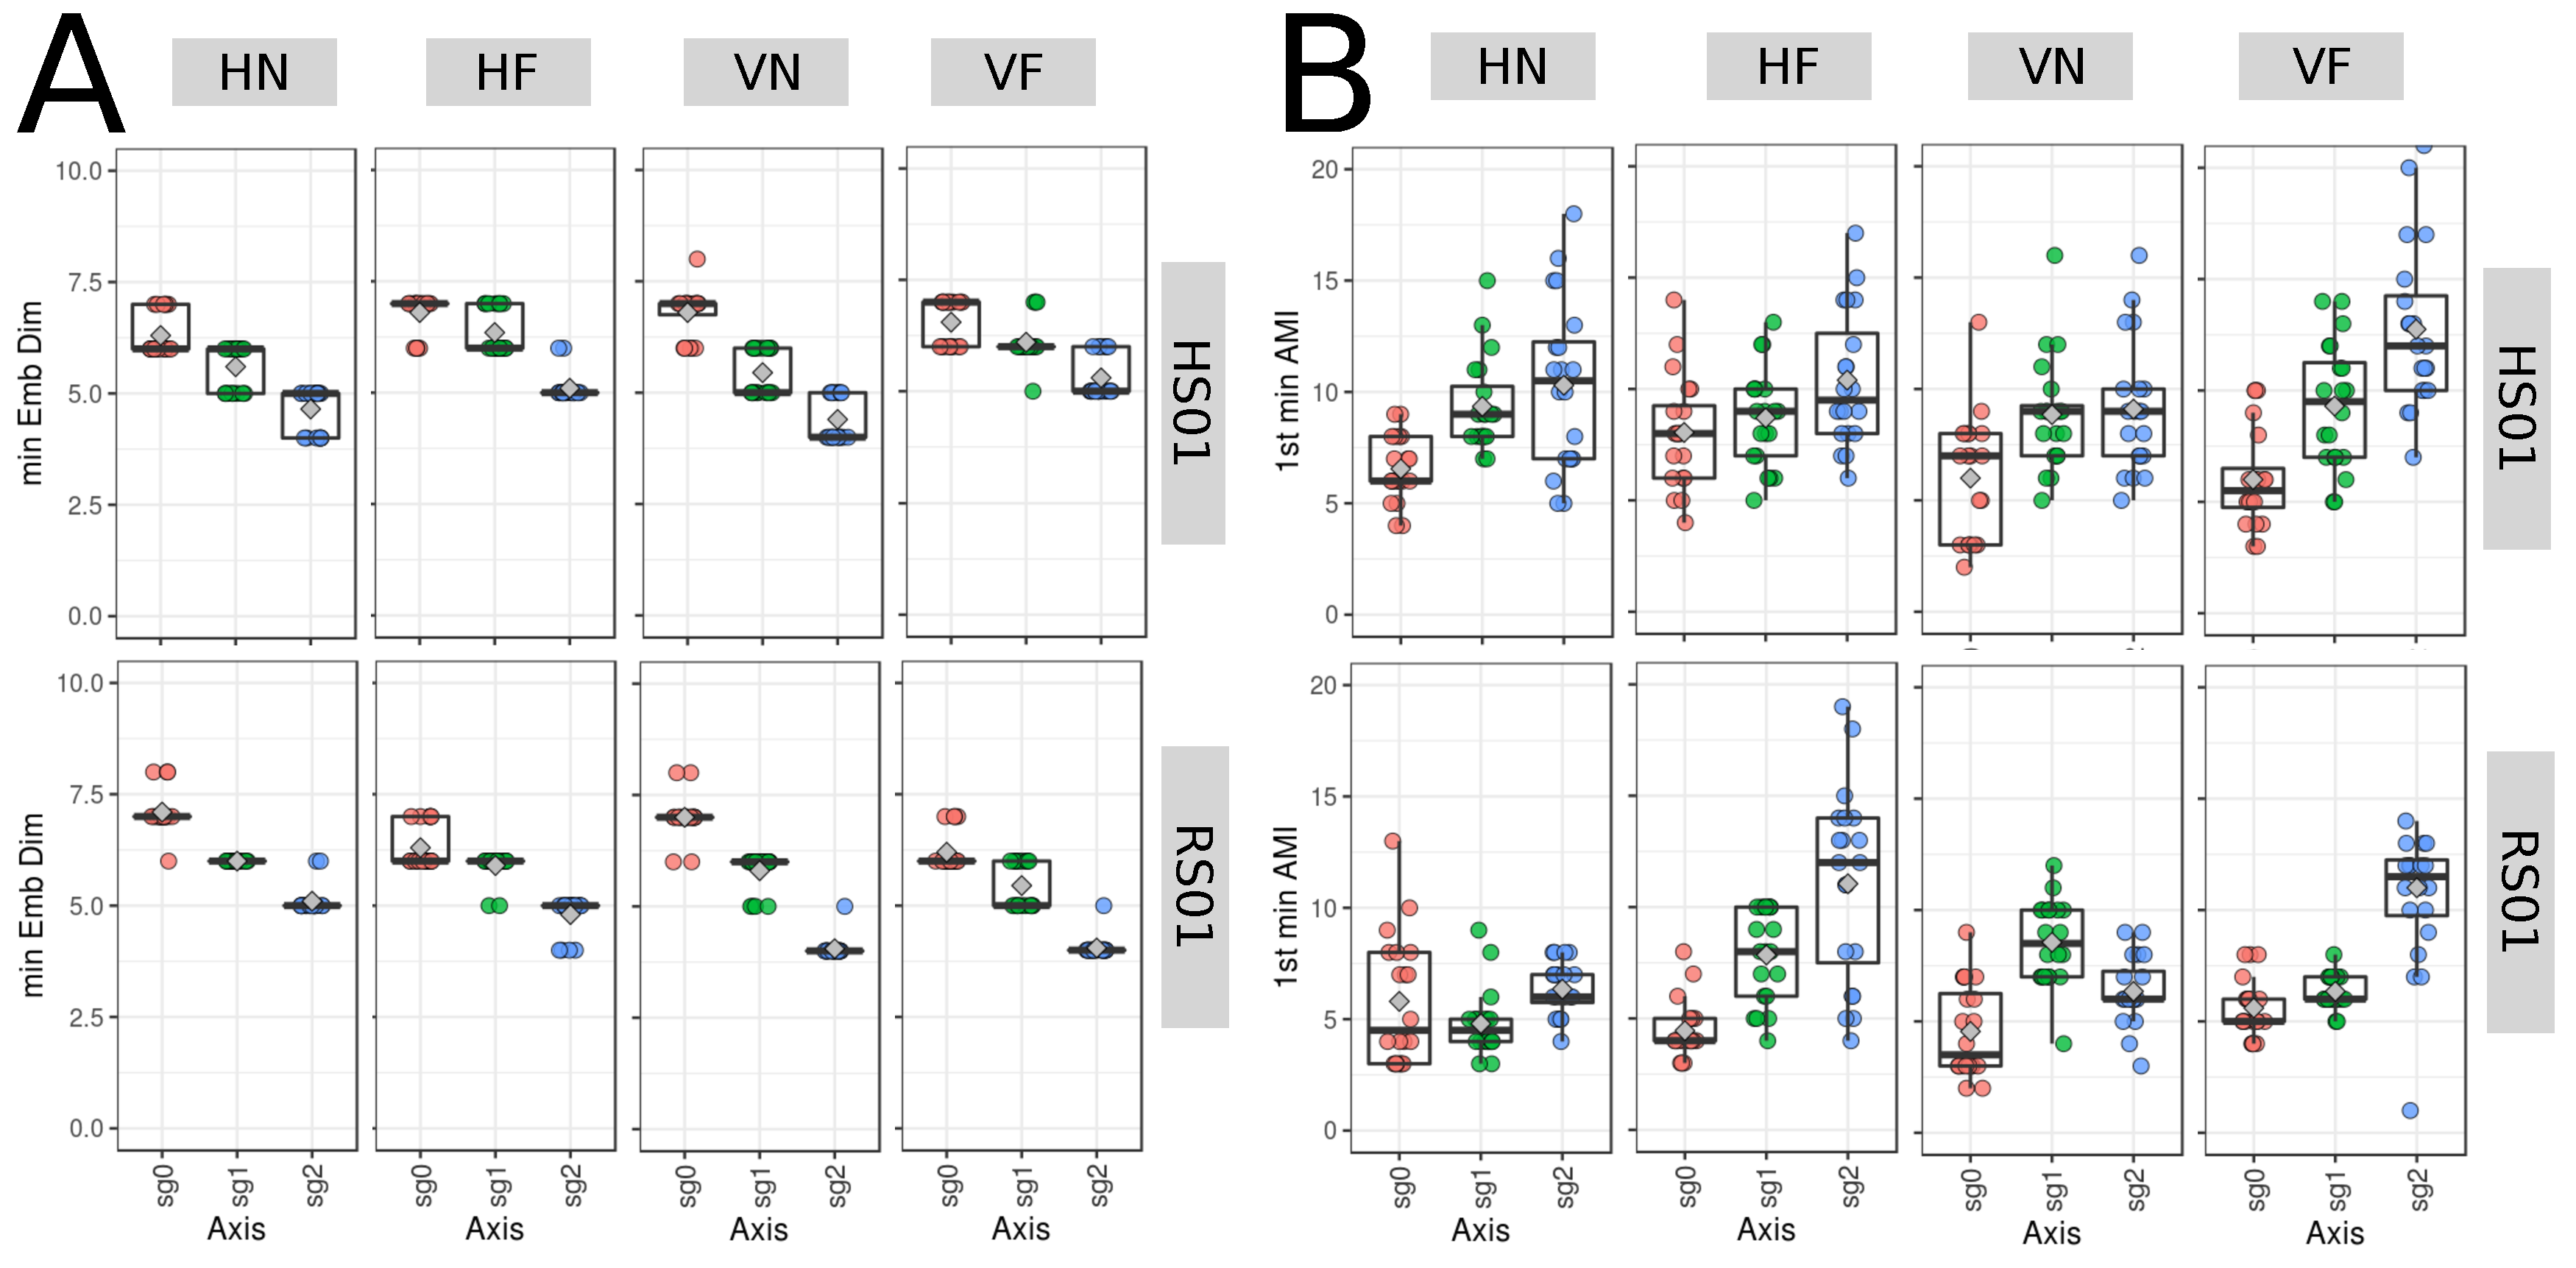
\includegraphics[width=1.0\textwidth]{fig-fig2.pdf}
	\caption{
	{\bf Box plots of minimum embedding parameters.} 
	Box plots of (A) minimum embedding dimensions 
	and (B) first minimum AMI values for 
	Horizontal Normal (HN), Horizontal Faster (HF),
	Vertical Normal (VN) and Vertical Faster (VF)
	with sensors attached to participants (HS01) and
	sensor attached to robot (RS01).
	Minimum embedding parameters are for twenty participants 
	($p01$ to $p20$) with three smoothed signals 
	(sg0: sg0zmuvGyroZ, sg1: sg1zmuvGyroZ and sg2: sg2zmuvGyroZ)
	and window length of 10-sec (500 samples).
	Code and data to reproduce the figure is available in \cite{srep2020}.
        }
    \label{fig:cao_ami}
\end{figure}
%%---------------------------------(FIGURE)------------------------------------

\subsubsection*{Uniform Time-Delay Embedding}
Using the overall embedding parameters ($\overline{m_0}=6$, $\overline{\tau_0}=8$), 
the first three axis of the rotated Principal Components Analysis (PCA) 
are shown for the reconstructed state spaces of horizontal (figures~\ref{fig:rsss}(A)) 
and vertical (figures~\ref{fig:rsss}(B)) arm movements. 
While visual inspection of these figures 
suggests differences in the trajectories of the reconstructed state spaces, 
we require an objective quantification to determine the extent of the differences.  
One approach could be use Euclidean distances from the origin for points in these 
trajectories, but this proved inconclusive and was not able to capture 
the dynamics of the trajectories. Consequently, we applied 
Recurrence Plots and Recurrence Quantification Analysis.
%%---------------------------------(FIGURE)-------------------------------------
\begin{figure}[ht]
\centering
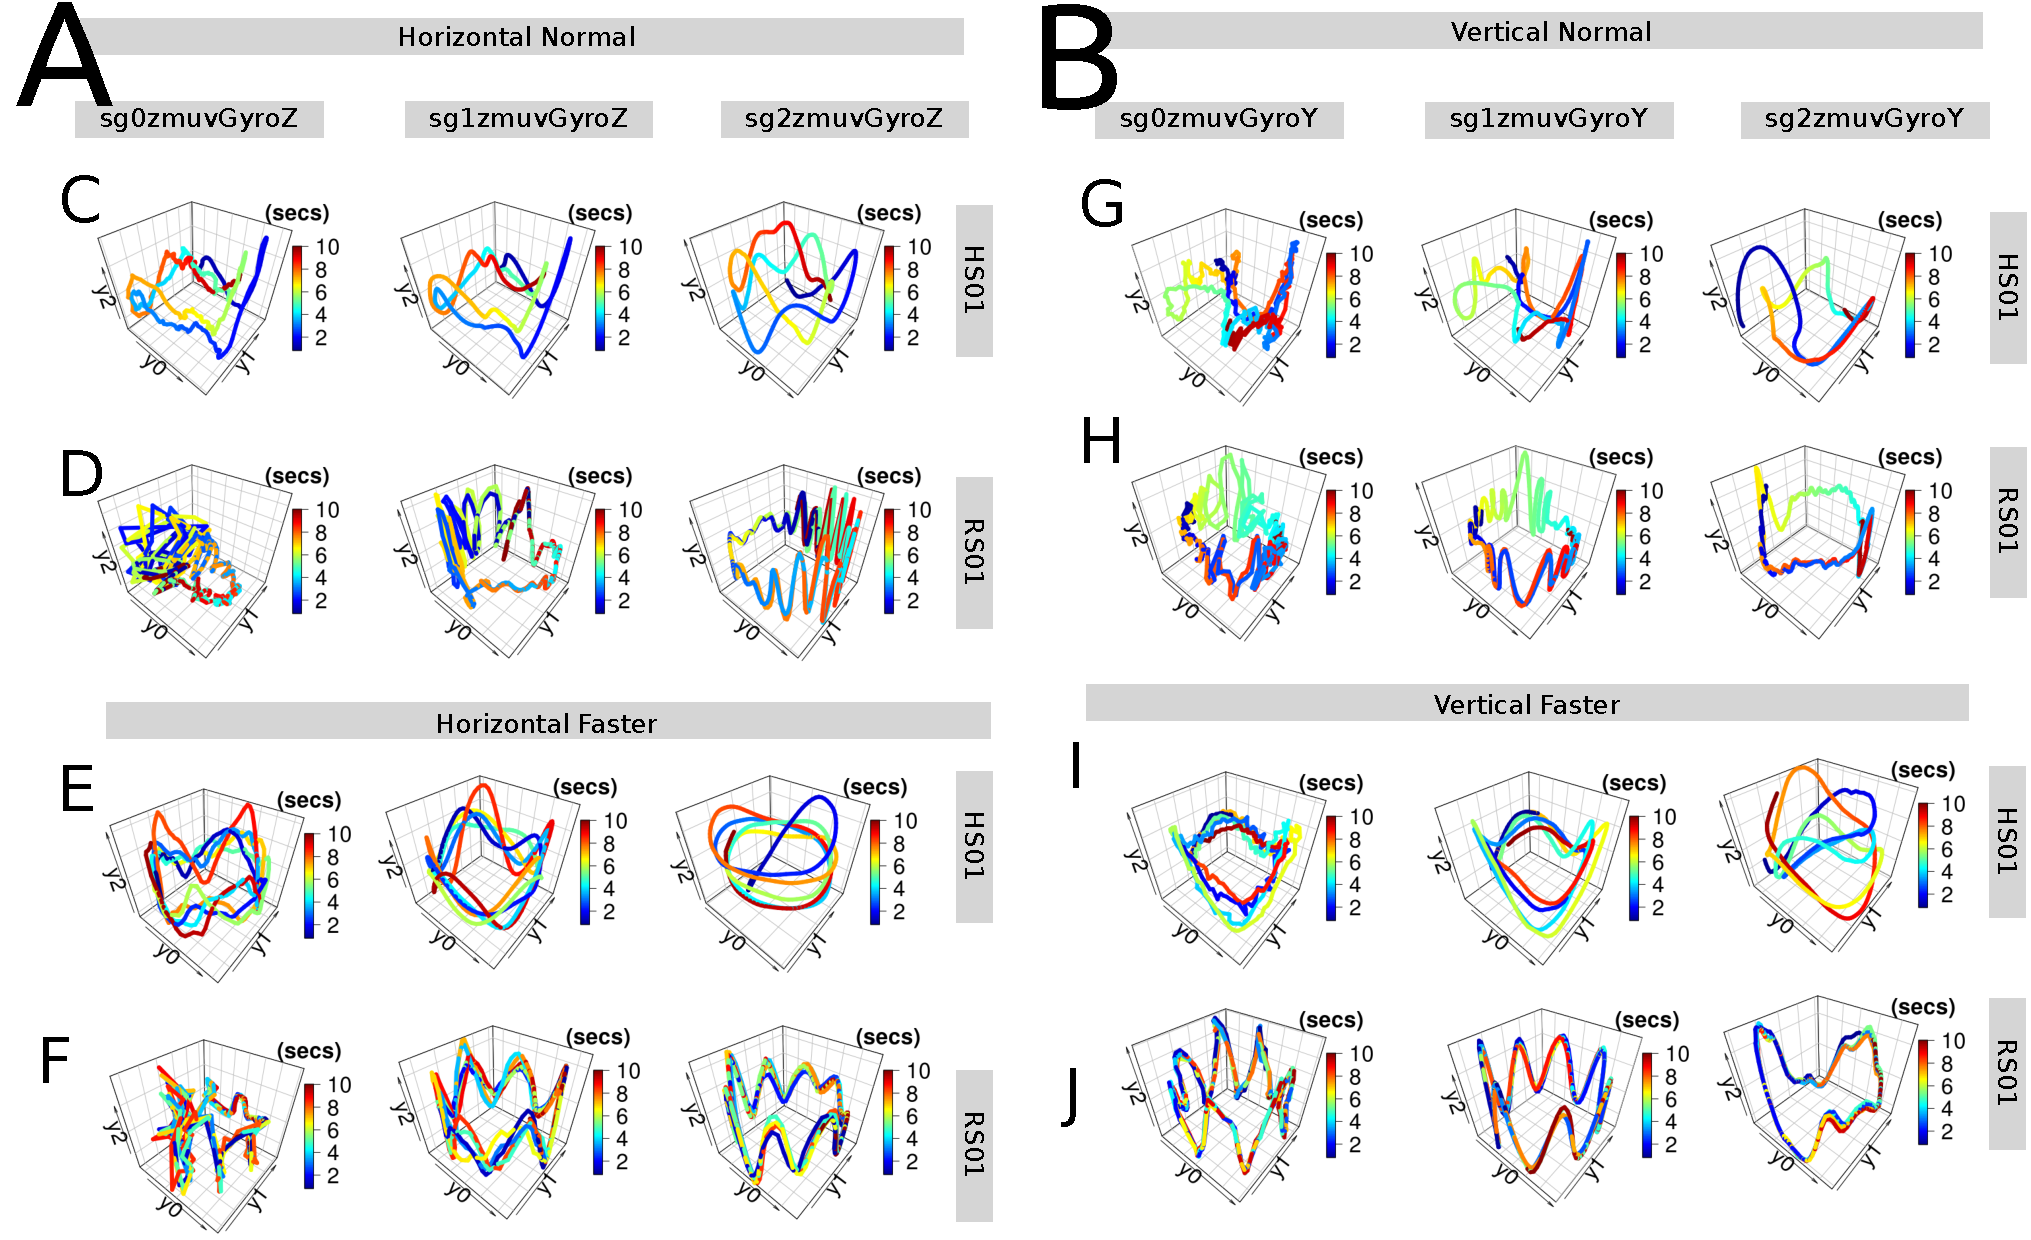
\includegraphics[width=1.0\textwidth]{fig-fig3.pdf}
\caption{
	{\bf RSSs for horizontal and vertical arm movements.}
	Reconstructed state spaces for time series for p01 of Figure \ref{fig:ts}.
	Reconstructed state spaces were computed with 
	embedding parameters 
	$\overline{m}_0=6$, $\overline{\tau}_0=8$
	for (A) horizontal and (B) vertical arm movements.
	Code and data to reproduce the figure is available in \cite{srep2020}.	
        }
    \label{fig:rsss}
\end{figure}
%%---------------------------------(FIGURE)------------------------------------



\subsection*{Recurrences Plots}
Using the average embedding parameters 
($\overline{m}_0=6$, $\overline{\tau}_0=8$) 
and an recurrence threshold of $\epsilon=1$.
As our interest is for dynamical transitions, 
there is little importance on the selection of $\epsilon$ which in this case
is 1. 
Recurrence Plots (RP) were computed for horizontal (figures~\ref{fig:rps}(A)) and 
vertical (figures~\ref{fig:rps}(B)) arm movements.
%%---------------------------------(FIGURE)-------------------------------------
\begin{figure}[ht]
\centering
\includegraphics[width=1.0\textwidth]{fig-fig4.pdf}
\caption{
	{\bf RPs for horizontal (A) and vertical (B) arm movements.}	
	Recurrence plots were computed with 
	embedding parameters 
	$\overline{m}_0=6$, $\overline{\tau}_0=8$, and $\epsilon=1$.
	Code and data to reproduce the figure is available in \cite{srep2020}.
        }
    \label{fig:rps}
\end{figure}
%%---------------------------------(FIGURE)------------------------------------

\subsection*{Recurrence Quantification Analysis} \label{ch6:rqas}
Four Recurrence Quantification Analysis metrics (
percentage recurrence, REC, representing the percentage of black dots in RP; 
percentage determinism, DET, representing the predictability of the RP; 
ratio of DET / REC, RATIO; Shannon entropy, ENTR) 
were computed using the same parameters as for RP.
%\subsubsection*{REC values}
Figure~\ref{fig:RQABP}(A) presents box plots of REC values, 
for HS01, are more spread for Slow (i.e., 5 seconds per movement) movements 
in Horizontal (HS) or Vertical (VS) than for Fast (i.e., 2 seconds per movement).  
This suggests greater variation between participants for the Slow movements.  
For RS01, there is little variation between Slow and Fast movement
(interquartile range of 0.01). 
In terms of smoothness, there seems little effect of HS01 but RS01 values 
do show affects of smoothness (see the incremental changes of mean values (rhombus)).
%\subsubsection*{DET values}
Figure \ref{fig:RQABP}(B) presents DET values and shows 
little difference for type of movement or performer.  
However, DET values are affected by changes in smoothness of the signal, 
particularly for Fast movement.
%\subsubsection*{RATIO values}
Figure \ref{fig:RQABP}(C) presents the ratio of DET / REC. 
These values, for the human performer, vary less for HN than for HF movement.  
Additionally, smoothness leads to a decrease in mean values for Fast movements.
%\subsubsection*{ENTR values}
Figure \ref{fig:RQABP}(D) shows ENTR values are higher for the human 
performer than the robot, and vary with the smoothness of the time-series.
%%---------------------------------(FIGURE)-------------------------------------
\begin{figure}
\centering
\includegraphics[width=1.0\textwidth]{fig-fig5.pdf}
    \caption
	[Box plots for RQA values]{
	{\bf Box plots for RQA metrics.}
	RQA metrics for (A) REC, (B) DET, (C) RATIO, and (D) ENTR of 
	20 participants performing HN, HF, VN and VF movements
	with sensors HS01, RS01 and three smoothed-normalised  
	time series (sg0, sg1 and sg2).
	RQA values were computed with 
	$\overline{m}_0=6$, $\overline{\tau}_0=8$, and $\epsilon=1$. 
	Code and data to reproduce the figure is available in \cite{srep2020}.
        }
    \label{fig:RQABP}
\end{figure}
%%---------------------------------(FIGURE)------------------------------------

%\subsection*{RQA metrics with fixed parameters}
%Considering that RQA metrics were computed with fixed embedding parameters 
%($m=6$ and $\tau=8$) and recurrence thresholds ($\epsilon=1$), we found 
%the following. REC values, which represents the \% of black points in the RPs, 
%were more affected with and increase in normal speed movements (HN and VN) 
%than faster movements (HF and VF) for the sensor attached to the participants 
%(HS01). Such decrease of REC values from normal speed to faster speed 
%movements is also presented in data from sensor attached to the robot (RS01), 
%and little can be said with regard to the dynamics of the time series coming 
%from RS01 (Fig \ref{fig:RQABP}A).
%Similarly, DET values, representing predictability and 
%organisation in the RPs, present little variation in the any of the time 
%series where little can be said (Fig \ref{fig:RQABP}B).
%In contrast, RATIO values, which represent 
%dynamic transitions, were more variable for faster movements (HF and VF) 
%than normal speed movements (HN and VN) with sensors attached to the 
%participants (HS01). For data coming from sensors attached to the robot 
%(RS01), RATIO values from horizontal movements (HN, HF) appear to vary 
%more than values coming from vertical movmentes (VN, VF) 
%(Fig \ref{fig:RQABP}C).
%With that, it can be said that RATIO values can represent a bit better
%than REC or DET metrics for the variability of imitation activities in 
%each of the conditions for time series.
%Similarly, ENTR values for HN were higher than values for HF
%and ENTR values varied more for sensor attached to participants 
%than ENTR values for sensors of the robot. It is evidently that 
%the higher the entropy the more complex the dynamics are, 
%however, ENTR values for HN appear a bit higher than HF values, 
%for which we believe this happens because of the structure the time series
%which appear more complex for HN than  HF movements which presented a 
%more consistence repetition (Fig \ref{fig:RQABP}D).


\subsection*{3D RQA ENTR}
As ENTR appeared to be have higher sensitivity than the other measures, 
we explored the impact of different embedding parameters 
$ \{ m \in \mathbb{R} | 1 \le m \le 10  \} $,
$  \{ \tau \in \mathbb{R} | 1 \le \tau \le 10  \} $ 
incrementing by 1 each run, with recurrence thresholds $\epsilon=1, 2, 3$ 
and levels of smoothness (sg0, sg1, sg2).  
Figure \ref{fig:RQA-IND} shows that increasing recurrence 
threshold leads to an increase in ENTR regardless of level of smoothness.  
Similarly, increasing level of smoothness will also increase ENTR (figure \ref{fig:RQA-IND}).
In terms of movement or performer, RQA ENTR decrease from Slow (HS, VS) to Fast (HF, VF) 
for both human (HS01) and (RS01) (Figures~\ref{fig:3dRQAENTR_sensoractivities}).
In terms of individual differences, for human participants, 
figure \ref{fig:3dRQAENTR_participantsactivities} compares p01, p02 and p03 (for illustrative purposes) --
both between each other and in comparison with the more consistent performance of the robot.  
In terms of window length (w100 (2s), w250 (5s), w500(10s), w750 (15s)), 
figure \ref{fig:3dRQAENTR_windowsactivities} shows that improvement in 
capture with number of samples, although this has less of an effect on RQA ENTR.

%%---------------------------------(FIGURE)-------------------------------------
\begin{figure}
\centering
\includegraphics[width=1.0\textwidth]{fig-rqa-epsilons.pdf}
    \caption
	[3D surface plots of RQA ENTR values]{
	{\bf 
	3D surface plots of RQA ENTR values for different recurrence threshold and smoothness levels.}
	RQA ENTR values are
	for embedding parameters
	$ \{ m \in \mathbb{R} | 0 \le m \le 10  \} $,
	$ \{ \tau \in \mathbb{R} | 0 \le \tau \le 10  \} $
	incrementing by one and three recurrence thresholds $\epsilon=1, 2, 3$.
	RQA ENTR values were computed with data from $p03$, sensor HS01, with 
	a window size of 10-secs (500 samples).
	Code and data to reproduce the figure is available in \cite{srep2020}.
        }
    \label{fig:RQA-IND}
\end{figure}
%%---------------------------------(FIGURE)------------------------------------

%%---------------------------------(FIGURE)-------------------------------------
\begin{figure}[ht]
\centering
\includegraphics[width=1.0\textwidth]{fig-rqa-sensors-activities.pdf}
    \caption{
	{\bf 3D surface plots of RQA ENTR values for different sensors and activities.}
	RQA ENTR values are for embedding parameters
	$ \{ m \in \mathbb{R} | 0 \le m \le 10  \}$,
	$ \{ \tau \in \mathbb{R} | 0 \le \tau \le 10  \}$
	with $\epsilon = 1 $ considering four activities 
	Horizontal Normal (HN), Horizontal Faster(HF), Vertical Normal(VN), and 
	Vertical Faster (VF) and sensors Human Sensor 01 (HS01) and 
	Robot Sensor (RS01).
	RQA ENTR values were computed from data of $p03$, sg0 and 
	window size of 10-secs (500 samples).
	Code and data to reproduce the figure is available in \cite{srep2020}.
       }
\label{fig:3dRQAENTR_sensoractivities}
\end{figure}
%%---------------------------------(FIGURE)-------------------------------------

%%---------------------------------(FIGURE)-------------------------------------
\begin{figure}[ht]
\centering
\includegraphics[width=0.9\textwidth]{fig-rqa-participants.pdf}
    \caption{
	{\bf 3D surface plots of RQA ENTR values for different participants, activities and sensors.}
	RQA ENTR values are for participants (p01, p02, and p03) 
	in the categories of 
	(A) Human Sensor 01 (HS01) and 
	(B) Robot Sensor 01 (RS01)
	considering embedding parameters
	$ \{ m \in \mathbb{R} | 0 \le m \le 10  \}$,
	$ \{ \tau \in \mathbb{R} | 0 \le \tau \le 10  \}$
	with $\epsilon = 1$ and four activities 
	Horizontal Normal (HN), Horizontal Faster(HF), Vertical Normal(VN), and 
	Vertical Faster (VF).
	RQA ENTR values were computed from data of sg0 and window size of 10-secs (500 samples).
	Code and data to reproduce the figure is available in \cite{srep2020}.
       }
\label{fig:3dRQAENTR_participantsactivities}
\end{figure}
%%---------------------------------(FIGURE)-------------------------------------

%%---------------------------------(FIGURE)-------------------------------------
\begin{figure}[ht]
\centering
\includegraphics[width=1.0\textwidth]{fig-rqa-windows}
    \caption{
	{\bf 3D surface plots of RQA ENTR values for different windows lengths and activities.}
	RQA ENTR values are for embedding parameters
	$ \{ m \in \mathbb{R} | 0 \le m \le 10  \}$,
	$ \{ \tau \in \mathbb{R} | 0 \le \tau \le 10  \}$, 
	with $\epsilon = 1 $ considering four 
	windows lengths (e.g., w100 (100 samples), w250 (250 samples),
	w500 (500 samples) and w750 (750 samples)) and
	four activities 
	Horizontal Normal (HN), Horizontal Faster(HF), Vertical Normal(VN), and 
	Vertical Faster (VF).
	RQA ENTR values were computed from data of $p01$ and sg0.
	Code and data to reproduce the figure is available in \cite{srep2020}.
       }
\label{fig:3dRQAENTR_windowsactivities}
\end{figure}
%%---------------------------------(FIGURE)-------------------------------------

To summarise this section of results, it can be said that computing
embedding parameters for individual structure of time-series 
data is already a solved problem \cite{frank2010, sama2013, bradley2015}. 
However, it has been shown the challenge of finding embedding parameters
for nonlinear dynamic tools that represent a set of different time-series data.
That said, we proposed the use of sample mean of the set of embedding parameters
for RSSs, RP and RQA to then noticed that the selection of recurrence 
threshold, $\epsilon$, is also an open problem.
For which, this work proposed the variation of recurrence thresholds 
and embedding parameters to show the relationships of these to different datasets 
(participants, activities, windows lengths and sensors).

%*******************************************************************************
%*******************************************************************************
%*******************************************************************************
\section*{Discussion}
While there are many approaches to estimating embedding parameters for nonlinear analysis, 
these can be influenced by the structure of the time-series data.   
We show that, for RSS, RP and RQA, the estimation of embedding parameters can be performed 
using a sample mean which, together with recurrence threshold, can be shown to be 
influenced by activity, performer, window length and smoothness of time-series.  
It is known that time-series from different sources and with different characteristics 
require different embedding parameters, and this can produce different RSS, RPs and RQAs. 
Although this work helps to understand the open problem of 
finding right balance among (i) the level of smoothness of the signal, 
(ii) the selection of recurrence thresholds and (iii) 
the range of embedding parameters, 
we have shown how RQA metrics can help to quantify movement variability.

\section*{Conclusions}
In this paper we show how the selection of nonlinear analysis tool  
(i.e., RSS, RP, RQA metrics) depends on what question one wishes to 
address with time-series data (e.g., predictability, organisation, dynamics, complexity).  
Time-series data characteristics (e.g., window length, smoothness), 
time-series structure (e.g., frequency, amplitude) and 
data source (e.g., sensor placement, performance, movement) all influence 
the results that nonlinear analysis methods can provide.
That said, it has been shown that the use of different characteristics of the data and 
their collection can help us visualise and quantify variability of movement using 
methods of nonlinear analysis.   
There remain limitations of nonlinear methods in 
relation to the estimation of parameters (e.g., recurrence threshold, embedding parameters) 
which reflect the dynamics of specific movement and performers, window length 
and structure of the time-series. 
We note that RQA DET seems to show low sensitivity 
to these differences, whereas REC and RATIO (primarily as a result of REC) show 
variation across performers and movements.   
RQA ENTR, with different recurrence thresholds, 
can quantify variation in the time-series data and offers the most appropriate means 
for analysing variability in movement to allow us to analyse individual differences 
between human performers.  
To then found out that RQA ENTR values with different recurrence 
thresholds were appropriate to quantify 
the different changes and variations of the characteristics of 
time-series data.
Therefore, the use of Shannon Entropy could be applied 
to analyse human participants who might vary in age, 
state of health, anthropometric features and capability to perform movement.

%% As a guideline references should be limited to 60 (this is not 
%% strictly enforced).
%\bibliography{sample}
%\bibliography{../references/references}
%\bibliography{references}
\input{main-arxiv.bbl}


\section*{Acknowledgements}

This work was funded by the University of Birmingham and the 
Mexican National Council of Science and Technology as part of 
Miguel Xochicale's PhD degree. I would like to thank to Dr. Dolores 
Columba Perez Flores and Prof. Martin J Russell for their helpful 
comments to polish the use of the language of mathematics and to 
Constantino Antonio Garcia Martinez et al. for developing the R 
package nonlinearTseries that help to accelerate the 
analysis of the nonlinear time series in this work.

\section*{Author contributions statement}
Contributions for this work of 
Miguel Xochicale (MX) and Chris Baber (CB) are as follows:
\begin{description}
\item[Conceptualisation] MX, CB
\item[Data Curation] MX
\item[Formal Analysis] MX
\item[Funding Acquisition] MX, CB
\item[Investigation] MX
\item[Methodology] MX
\item[Project Administration] MX
\item[Resources] CB
\item[Software] MX
\item[Supervision] CB
\item[Validation] MX
\item[Verification] MX
\item[Writing - Original Draft Preparation] MX
\item[Writing - Review] MX, CB
\item[Writing - Editing] MX
\end{description}

%
%\section*{Additional information}
%
%To include, in this order: \textbf{Accession codes} 
%(where applicable); \textbf{Competing interests} (mandatory statement). 
%
%The corresponding author is responsible for submitting a 
%\href{http://www.nature.com/srep/policies/index.html#competing}{competing interests statement} on 
%behalf of all authors of the paper. This statement must be included 
%in the submitted article file.
%
%\begin{figure}[ht]
%\centering
%\includegraphics[width=\linewidth]{stream}
%\caption{Legend (350 words max). Example legend text.}
%\label{fig:stream}
%\end{figure}

%\begin{table}[ht]
%\centering
%\begin{tabular}{|l|l|l|}
%\hline
%Condition & n & p \\
%\hline
%A & 5 & 0.1 \\
%\hline
%B & 10 & 0.01 \\
%\hline
%\end{tabular}
%\caption{\label{tab:example}Legend (350 words max). Example legend text.}
%\end{table}
%
%Figures and tables can be referenced in LaTeX using the ref command, 
%e.g. Figure \ref{fig:stream} and Table \ref{tab:example}.

\end{document}



\section*{Acknowledgements}

This work was funded by the University of Birmingham and the 
Mexican National Council of Science and Technology as part of 
Miguel Xochicale's PhD degree. I would like to thank to Dr. Dolores 
Columba Perez Flores and Prof. Martin J Russell for their helpful 
comments to polish the use of the language of mathematics and to 
Constantino Antonio Garcia Martinez et al. for developing the R 
package nonlinearTseries that help to accelerate the 
analysis of the nonlinear time series in this work.

\section*{Author contributions statement}
Contributions for this work of 
Miguel Xochicale (MX) and Chris Baber (CB) are as follows:
\begin{description}
\item[Conceptualisation] MX, CB
\item[Data Curation] MX
\item[Formal Analysis] MX
\item[Funding Acquisition] MX, CB
\item[Investigation] MX
\item[Methodology] MX
\item[Project Administration] MX
\item[Resources] CB
\item[Software] MX
\item[Supervision] CB
\item[Validation] MX
\item[Verification] MX
\item[Writing - Original Draft Preparation] MX
\item[Writing - Review] MX, CB
\item[Writing - Editing] MX
\end{description}

%
%\section*{Additional information}
%
%To include, in this order: \textbf{Accession codes} 
%(where applicable); \textbf{Competing interests} (mandatory statement). 
%
%The corresponding author is responsible for submitting a 
%\href{http://www.nature.com/srep/policies/index.html#competing}{competing interests statement} on 
%behalf of all authors of the paper. This statement must be included 
%in the submitted article file.
%
%\begin{figure}[ht]
%\centering
%\includegraphics[width=\linewidth]{stream}
%\caption{Legend (350 words max). Example legend text.}
%\label{fig:stream}
%\end{figure}

%\begin{table}[ht]
%\centering
%\begin{tabular}{|l|l|l|}
%\hline
%Condition & n & p \\
%\hline
%A & 5 & 0.1 \\
%\hline
%B & 10 & 0.01 \\
%\hline
%\end{tabular}
%\caption{\label{tab:example}Legend (350 words max). Example legend text.}
%\end{table}
%
%Figures and tables can be referenced in LaTeX using the ref command, 
%e.g. Figure \ref{fig:stream} and Table \ref{tab:example}.

\end{document}



\section*{Acknowledgements}

This work was funded by the University of Birmingham and the 
Mexican National Council of Science and Technology as part of 
Miguel Xochicale's PhD degree. I would like to thank to Dr. Dolores 
Columba Perez Flores and Prof. Martin J Russell for their helpful 
comments to polish the use of the language of mathematics and to 
Constantino Antonio Garcia Martinez et al. for developing the R 
package nonlinearTseries that help to accelerate the 
analysis of the nonlinear time series in this work.

\section*{Author contributions statement}
Contributions for this work of 
Miguel Xochicale (MX) and Chris Baber (CB) are as follows:
\begin{description}
\item[Conceptualisation] MX, CB
\item[Data Curation] MX
\item[Formal Analysis] MX
\item[Funding Acquisition] MX, CB
\item[Investigation] MX
\item[Methodology] MX
\item[Project Administration] MX
\item[Resources] CB
\item[Software] MX
\item[Supervision] CB
\item[Validation] MX
\item[Verification] MX
\item[Writing - Original Draft Preparation] MX
\item[Writing - Review] MX, CB
\item[Writing - Editing] MX
\end{description}

%
%\section*{Additional information}
%
%To include, in this order: \textbf{Accession codes} 
%(where applicable); \textbf{Competing interests} (mandatory statement). 
%
%The corresponding author is responsible for submitting a 
%\href{http://www.nature.com/srep/policies/index.html#competing}{competing interests statement} on 
%behalf of all authors of the paper. This statement must be included 
%in the submitted article file.
%
%\begin{figure}[ht]
%\centering
%\includegraphics[width=\linewidth]{stream}
%\caption{Legend (350 words max). Example legend text.}
%\label{fig:stream}
%\end{figure}

%\begin{table}[ht]
%\centering
%\begin{tabular}{|l|l|l|}
%\hline
%Condition & n & p \\
%\hline
%A & 5 & 0.1 \\
%\hline
%B & 10 & 0.01 \\
%\hline
%\end{tabular}
%\caption{\label{tab:example}Legend (350 words max). Example legend text.}
%\end{table}
%
%Figures and tables can be referenced in LaTeX using the ref command, 
%e.g. Figure \ref{fig:stream} and Table \ref{tab:example}.

\end{document}



\section*{Acknowledgements}

This work was funded by the University of Birmingham and the 
Mexican National Council of Science and Technology as part of 
Miguel Xochicale's PhD degree. I would like to thank to Dr. Dolores 
Columba Perez Flores and Prof. Martin J Russell for their helpful 
comments to polish the use of the language of mathematics and to 
Constantino Antonio Garcia Martinez et al. for developing the R 
package nonlinearTseries that help to accelerate the 
analysis of the nonlinear time series in this work.

\section*{Author contributions statement}
Contributions for this work of 
Miguel Xochicale (MX) and Chris Baber (CB) are as follows:
\begin{description}
\item[Conceptualisation] MX, CB
\item[Data Curation] MX
\item[Formal Analysis] MX
\item[Funding Acquisition] MX, CB
\item[Investigation] MX
\item[Methodology] MX
\item[Project Administration] MX
\item[Resources] CB
\item[Software] MX
\item[Supervision] CB
\item[Validation] MX
\item[Verification] MX
\item[Writing - Original Draft Preparation] MX
\item[Writing - Review] MX, CB
\item[Writing - Editing] MX
\end{description}

%
%\section*{Additional information}
%
%To include, in this order: \textbf{Accession codes} 
%(where applicable); \textbf{Competing interests} (mandatory statement). 
%
%The corresponding author is responsible for submitting a 
%\href{http://www.nature.com/srep/policies/index.html#competing}{competing interests statement} on 
%behalf of all authors of the paper. This statement must be included 
%in the submitted article file.
%
%\begin{figure}[ht]
%\centering
%\includegraphics[width=\linewidth]{stream}
%\caption{Legend (350 words max). Example legend text.}
%\label{fig:stream}
%\end{figure}

%\begin{table}[ht]
%\centering
%\begin{tabular}{|l|l|l|}
%\hline
%Condition & n & p \\
%\hline
%A & 5 & 0.1 \\
%\hline
%B & 10 & 0.01 \\
%\hline
%\end{tabular}
%\caption{\label{tab:example}Legend (350 words max). Example legend text.}
%\end{table}
%
%Figures and tables can be referenced in LaTeX using the ref command, 
%e.g. Figure \ref{fig:stream} and Table \ref{tab:example}.

\end{document}
